\chapter{Images and Plots}

All the diagrams, plots, and natural images are included in this chapter.


%%%%%%%%%%%%%%%%%%%%%%%%%%%%%%%%%%%%%%%%%%%%%%%%%%%%%%%%%%%%%
%%%%%%%%%%%% Phase in Fourier Reconstruction %%%%%%%%%%%%%%%%
%%%%%%%%%%%%%%%%%%%%%%%%%%%%%%%%%%%%%%%%%%%%%%%%%%%%%%%%%%%%%
\afterpage{%
  % \clearpage % Start a new page
  % \thispagestyle{empty} % No header/footer on this page
  \begin{figure}[!htbp]
    \centering
	\captionsetup{justification=centering}
    \includegraphics[width=1.0\textwidth,height=65em]{./images/phase_importance/phase_importance_comparison.png}
    \caption{The Importance of Phase in Fourier Reconstruction \cite{Oppenheim1981}\cite{Shechtman2015} }
    \label{fig:sat_phone_vs_job_hunting}
  \end{figure}
  % \clearpage % End the page
}

%%%%%%%%%%%%%%%%%%%%%%%%%%%%%%%%%%%%%%%%%%%%%%%%%%%%%%%%%%%%%
%%%%%%%%%%% WF vs TWF vs RWF vs IRWF vs IMRWF  %%%%%%%%%%%%%%
%%%%%%%%%%%%%%%%%%%%%%%%%%%%%%%%%%%%%%%%%%%%%%%%%%%%%%%%%%%%%
\afterpage{%
%   \clearpage % Start a new page
  \begin{figure}[!htbp]
    \centering
	\captionsetup{justification=centering}
  % \begin{turn}{-90}
    % This file was created with tikzplotlib v0.10.1.
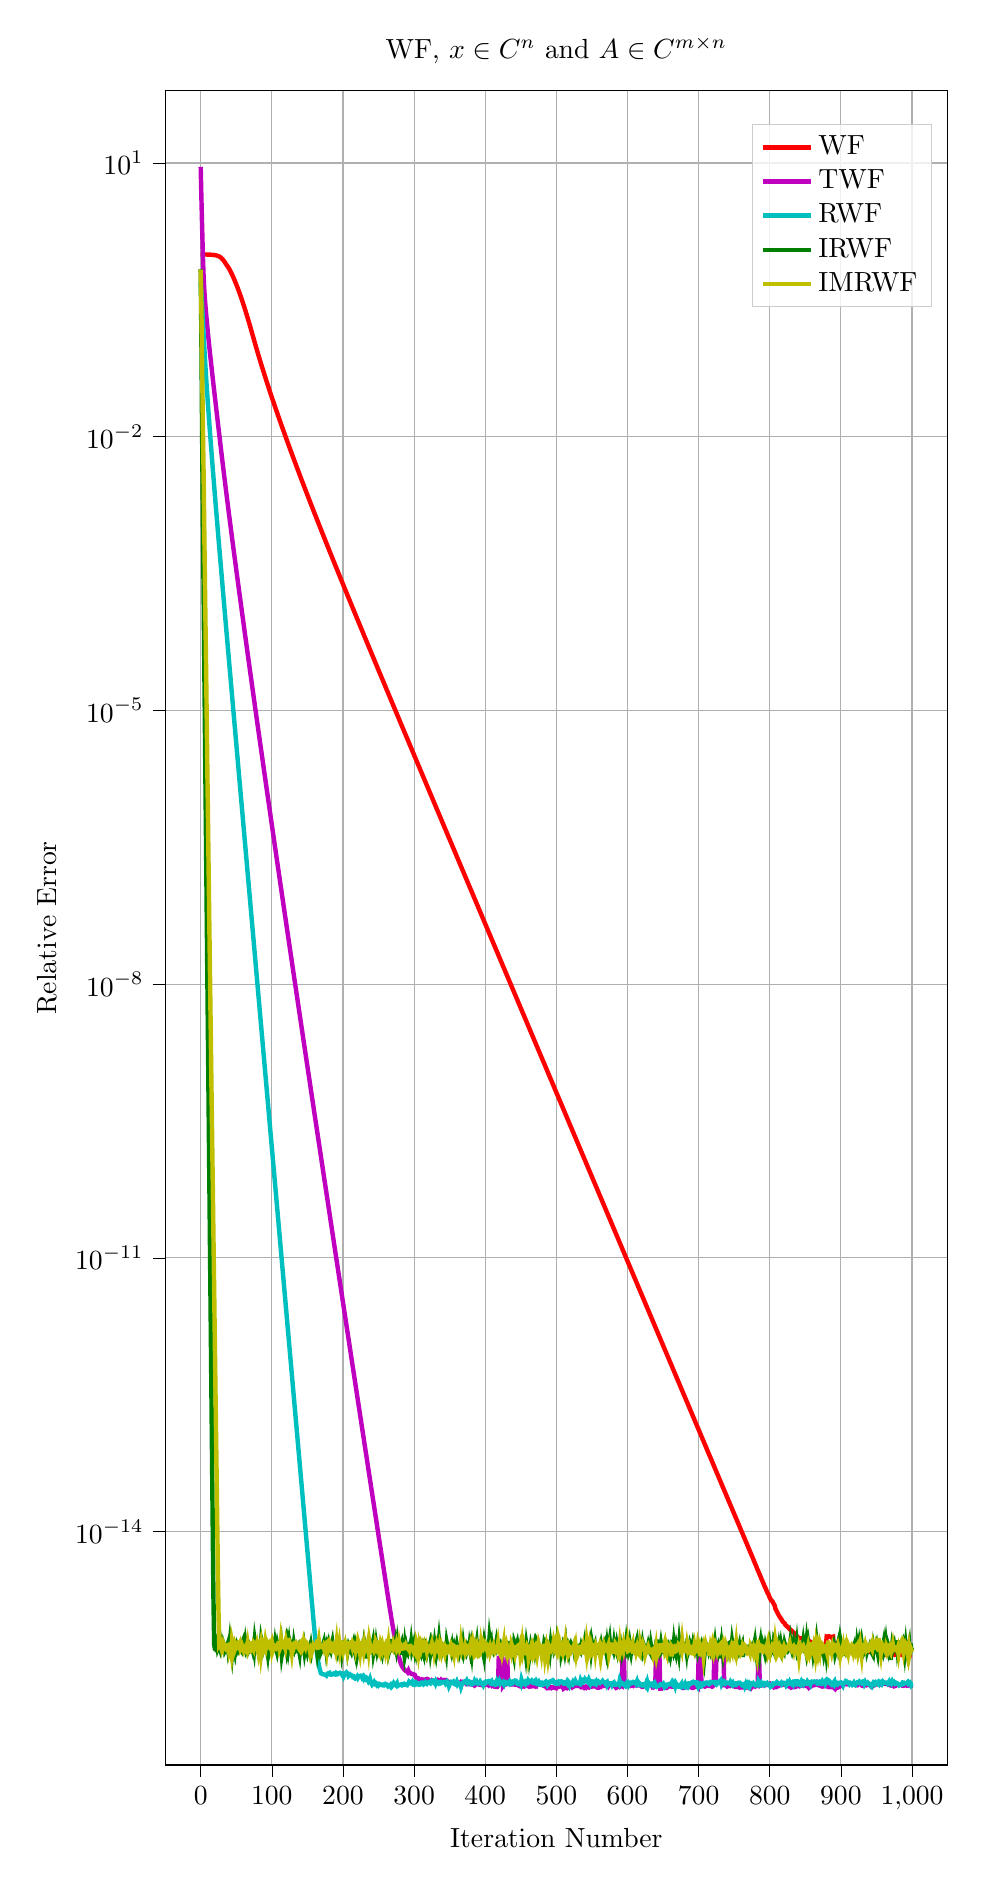
\begin{tikzpicture}

  \definecolor{darkgray176}{RGB}{176,176,176}
  \definecolor{darkturquoise0191191}{RGB}{0,191,191}
  \definecolor{darkviolet1910191}{RGB}{191,0,191}
  \definecolor{goldenrod1911910}{RGB}{191,191,0}
  \definecolor{green01270}{RGB}{0,127,0}
  \definecolor{lightgray204}{RGB}{204,204,204}
  
  \begin{axis}[
  width = 0.95\textwidth,
  height = 65em,
  legend cell align={left},
  legend style={fill opacity=0.8, draw opacity=1, text opacity=1, draw=lightgray204},
  log basis y={10},
  tick align=outside,
  tick pos=left,
  title={\ac{WF}, $\boldsymbol{x} \in \mathbb{C}^n$ and $\boldsymbol{A} \in \mathbb{C}^{m \times n}$},
  x grid style={darkgray176},
  xlabel={Iteration Number},
  xmajorgrids,
  xmin=-50, xmax=1050,
  xtick style={color=black},
  y grid style={darkgray176},
  ylabel={Relative Error},
  ymajorgrids,
  ymin=2.75985430994154e-17, ymax=62.0823981613045,
  ymode=log,
  ytick style={color=black},
  ytick={1e-20,1e-17,1e-14,1e-11,1e-08,1e-05,0.01,10,10000,10000000},
  yticklabels={
    \(\displaystyle {10^{-20}}\),
    \(\displaystyle {10^{-17}}\),
    \(\displaystyle {10^{-14}}\),
    \(\displaystyle {10^{-11}}\),
    \(\displaystyle {10^{-8}}\),
    \(\displaystyle {10^{-5}}\),
    \(\displaystyle {10^{-2}}\),
    \(\displaystyle {10^{1}}\),
    \(\displaystyle {10^{4}}\),
    \(\displaystyle {10^{7}}\)
  }
  ]
  \addplot [ultra thick, red]
  table {%
  0 0.994928926814044
  1 0.994889801322374
  2 0.9948110924516
  3 0.994691466369448
  4 0.994528680803586
  5 0.994319520349983
  6 0.994059697282739
  7 0.993743713960874
  8 0.993364681166018
  9 0.99291408469794
  10 0.99238149021208
  11 0.991754173510616
  12 0.991016660202542
  13 0.990150154746145
  14 0.989131834331593
  15 0.987933977883915
  16 0.986522894863765
  17 0.984857613027563
  18 0.982888279981832
  19 0.980554232400566
  20 0.977781693251186
  21 0.974481078736186
  22 0.970543946166553
  23 0.965839714782401
  24 0.960212483025328
  25 0.953478612680687
  26 0.945426352857586
  27 0.935819773014247
  28 0.924410804833137
  29 0.910965245406331
  30 0.895310514848173
  31 0.877412414927472
  32 0.8574790408091
  33 0.836061583485434
  34 0.814066989041492
  35 0.792548617852663
  36 0.772220197703635
  37 0.752963807003155
  38 0.733884825150826
  39 0.714025149360269
  40 0.693000090215385
  41 0.670983329059018
  42 0.648347450466976
  43 0.625419926827566
  44 0.602424917387903
  45 0.579505372599469
  46 0.556755516118967
  47 0.534244009133946
  48 0.512027351311858
  49 0.490156601962512
  50 0.468680026862704
  51 0.447643427565718
  52 0.427089303002292
  53 0.407055595991651
  54 0.387574510848114
  55 0.368671700155578
  56 0.350365974182052
  57 0.332669564729723
  58 0.315588871540356
  59 0.299125541257913
  60 0.283277687488603
  61 0.268041061017969
  62 0.253410016865008
  63 0.239378186034542
  64 0.225938827429917
  65 0.213084894021537
  66 0.200808886996663
  67 0.189102588781784
  68 0.177956762820528
  69 0.167360890763906
  70 0.157302993482034
  71 0.147769557469904
  72 0.138745567292102
  73 0.130214629950445
  74 0.122194207531744
  75 0.114715875920365
  76 0.107742229478165
  77 0.101237897922956
  78 0.0951695913947969
  79 0.0895061061468954
  80 0.0842182976224538
  81 0.0792790265389404
  82 0.0746630839736293
  83 0.0703471012787694
  84 0.066309450049261
  85 0.0625301365507346
  86 0.0589906941541068
  87 0.0556740765096845
  88 0.0525645534779521
  89 0.0496476112332159
  90 0.0469098574701613
  91 0.0443389322623374
  92 0.0419234248314952
  93 0.0396527962723245
  94 0.0375173081239108
  95 0.0355079565741621
  96 0.0336164120154638
  97 0.0318349636297665
  98 0.0301564686618362
  99 0.0285743060347035
  100 0.0270823339669686
  101 0.0256748512641327
  102 0.0243465619730173
  103 0.0230925431077118
  104 0.0219082151760497
  105 0.0207893152563853
  106 0.0197318723948189
  107 0.018732185112554
  108 0.0177868008315372
  109 0.0168924970437706
  110 0.0160462640656537
  111 0.0152452892334008
  112 0.0144869424090251
  113 0.013768762678642
  114 0.0130884461359962
  115 0.0124438346542306
  116 0.0118329055580804
  117 0.0112537621169671
  118 0.0107046247869587
  119 0.0101838231363354
  120 0.0096897883956122
  121 0.0092210465783894
  122 0.00877621212438497
  123 0.00835398202050114
  124 0.00795313035983832
  125 0.00757250330223691
  126 0.00721101440323959
  127 0.00686764028135981
  128 0.0065414165962461
  129 0.00623143431277761
  130 0.00593683622833792
  131 0.00565681374251461
  132 0.00539060385028484
  133 0.00513748634138757
  134 0.00489678119006975
  135 0.00466784612074251
  136 0.00445007433630639
  137 0.00424289239701482
  138 0.00404575823875369
  139 0.00385815932053163
  140 0.00367961089180879
  141 0.00350965437105164
  142 0.00334785582759109
  143 0.00319380455949235
  144 0.00304711176071818
  145 0.00290740927139265
  146 0.00277434840545062
  147 0.00264759885039635
  148 0.00252684763429543
  149 0.00241179815549035
  150 0.00230216927086696
  151 0.0021976944388062
  152 0.00209812091323959
  153 0.00200320898548528
  154 0.00191273127078192
  155 0.0018264720366558
  156 0.00174422657046002
  157 0.00166580058361045
  158 0.00159100965021516
  159 0.00151967867795246
  160 0.00145164140919975
  161 0.00138673995055006
  162 0.00132482432897895
  163 0.00126575207304
  164 0.00120938781757494
  165 0.00115560293052348
  166 0.00110427516051059
  167 0.00105528830397483
  168 0.0010085318906801
  169 0.000963900886528458
  170 0.000921295412659157
  171 0.000880620479884064
  172 0.00084178573756855
  173 0.000804705236123118
  174 0.000769297202321748
  175 0.000735483826713012
  176 0.000703191062432883
  177 0.000672348434771962
  178 0.00064288886088833
  179 0.000614748479094179
  180 0.000587866487178512
  181 0.000562184989260636
  182 0.000537648850698864
  183 0.000514205560607537
  184 0.000491805101560791
  185 0.000470399826087643
  186 0.000449944339584679
  187 0.000430395389295337
  188 0.00041171175902468
  189 0.000393854169277587
  190 0.000376785182526566
  191 0.000360469113331986
  192 0.000344871943053163
  193 0.000329961238904074
  194 0.000315706077121021
  195 0.000302076970022713
  196 0.000289045796755883
  197 0.000276585737530783
  198 0.000264671211161965
  199 0.000253277815740333
  200 0.000242382272271271
  201 0.000231962371123978
  202 0.000221996921144582
  203 0.000212465701294335
  204 0.000203349414681508
  205 0.000194629644863001
  206 0.000186288814298413
  207 0.000178310144845165
  208 0.000170677620190302
  209 0.000163375950119054
  210 0.000156390536526759
  211 0.000149707441084836
  212 0.000143313354476758
  213 0.00013719556712447
  214 0.000131341941329614
  215 0.000125740884758247
  216 0.000120381325201443
  217 0.000115252686547569
  218 0.000110344865905651
  219 0.000105648211822192
  220 0.000101153503536986
  221 9.68519312263095e-05
  222 9.27350771843695e-05
  223 8.87948978966866e-05
  224 8.50237069614426e-05
  225 8.1414158816783e-05
  226 7.79592332347465e-05
  227 7.46522205440832e-05
  228 7.14867075463782e-05
  229 6.84565640916957e-05
  230 6.55559302814271e-05
  231 6.27792042682607e-05
  232 6.01210306239292e-05
  233 5.75762892476625e-05
  234 5.51400847888807e-05
  235 5.28077365598184e-05
  236 5.05747689140638e-05
  237 4.84369020691682e-05
  238 4.63900433516732e-05
  239 4.44302788447578e-05
  240 4.25538654190495e-05
  241 4.07572231285269e-05
  242 3.90369279542499e-05
  243 3.73897048793828e-05
  244 3.5812421279848e-05
  245 3.43020806158338e-05
  246 3.28558164098592e-05
  247 3.14708864982058e-05
  248 3.01446675425297e-05
  249 2.88746497898422e-05
  250 2.76584320691654e-05
  251 2.64937170136427e-05
  252 2.53783064979009e-05
  253 2.43100972805772e-05
  254 2.32870768424586e-05
  255 2.23073194111884e-05
  256 2.13689821639752e-05
  257 2.04703016001941e-05
  258 1.96095900758276e-05
  259 1.8785232492542e-05
  260 1.79956831342278e-05
  261 1.72394626442257e-05
  262 1.6515155136817e-05
  263 1.58214054369526e-05
  264 1.5156916442257e-05
  265 1.45204466018819e-05
  266 1.39108075066469e-05
  267 1.33268615858532e-05
  268 1.27675199055268e-05
  269 1.22317400636308e-05
  270 1.17185241781542e-05
  271 1.12269169634544e-05
  272 1.07560038910274e-05
  273 1.03049094313477e-05
  274 9.87279537230909e-06
  275 9.45885921150675e-06
  276 9.06233261898803e-06
  277 8.68247996692533e-06
  278 8.31859692353184e-06
  279 7.97000910853766e-06
  280 7.63607080696653e-06
  281 7.31616373904266e-06
  282 7.00969588359499e-06
  283 6.71610035270797e-06
  284 6.43483431493247e-06
  285 6.16537796567527e-06
  286 5.90723354170894e-06
  287 5.65992437881806e-06
  288 5.42299400999908e-06
  289 5.19600530267708e-06
  290 4.97853963328207e-06
  291 4.7701960974222e-06
  292 4.5705907541438e-06
  293 4.37935590282112e-06
  294 4.19613939110675e-06
  295 4.0206039528615e-06
  296 3.85242657435645e-06
  297 3.69129788787673e-06
  298 3.53692159135241e-06
  299 3.38901389292161e-06
  300 3.24730297929986e-06
  301 3.11152850695441e-06
  302 2.9814411151605e-06
  303 2.85680195981666e-06
  304 2.7373822673436e-06
  305 2.62296290752867e-06
  306 2.51333398474704e-06
  307 2.40829444667254e-06
  308 2.30765170956247e-06
  309 2.21122129971287e-06
  310 2.11882651012163e-06
  311 2.03029807182836e-06
  312 1.94547383920507e-06
  313 1.86419848877537e-06
  314 1.78632323079471e-06
  315 1.71170553302934e-06
  316 1.64020885648817e-06
  317 1.57170240218907e-06
  318 1.5060608688799e-06
  319 1.44316422079782e-06
  320 1.38289746568333e-06
  321 1.32515044181081e-06
  322 1.26981761427356e-06
  323 1.21679787998614e-06
  324 1.16599438076968e-06
  325 1.11731432442261e-06
  326 1.07066881348508e-06
  327 1.02597268107283e-06
  328 9.83144333871808e-07
  329 9.42105601568395e-07
  330 9.027815928249e-07
  331 8.65100557242981e-07
  332 8.28993753193294e-07
  333 7.94395321318817e-07
  334 7.61242163180492e-07
  335 7.29473825220449e-07
  336 6.99032387626029e-07
  337 6.6986235775119e-07
  338 6.41910568086543e-07
  339 6.15126078612611e-07
  340 5.8946008323779e-07
  341 5.64865820102195e-07
  342 5.41298485760461e-07
  343 5.18715152985142e-07
  344 4.97074691898391e-07
  345 4.76337694700636e-07
  346 4.56466403178503e-07
  347 4.3742463969459e-07
  348 4.1917774070511e-07
  349 4.01692493364037e-07
  350 3.84937074614267e-07
  351 3.68880992913001e-07
  352 3.53495032451632e-07
  353 3.38751199560624e-07
  354 3.24622671638312e-07
  355 3.11083747906799e-07
  356 2.98109802474763e-07
  357 2.85677239308346e-07
  358 2.7376344907862e-07
  359 2.6234676776523e-07
  360 2.51406437152818e-07
  361 2.40922566800919e-07
  362 2.30876097812313e-07
  363 2.21248767892498e-07
  364 2.12023078071587e-07
  365 2.0318226073883e-07
  366 1.94710249030568e-07
  367 1.86591647438224e-07
  368 1.78811703868386e-07
  369 1.71356282498381e-07
  370 1.64211838167535e-07
  371 1.57365391574898e-07
  372 1.50804505654477e-07
  373 1.44517262854604e-07
  374 1.38492243446779e-07
  375 1.32718504607895e-07
  376 1.27185560662593e-07
  377 1.21883363765551e-07
  378 1.16802285709198e-07
  379 1.11933100351737e-07
  380 1.07266966779569e-07
  381 1.02795413292624e-07
  382 9.85103218269272e-08
  383 9.44039133069121e-08
  384 9.04687334256843e-08
  385 8.66976390421355e-08
  386 8.3083785223591e-08
  387 7.96206127564723e-08
  388 7.630183622648e-08
  389 7.31214325692232e-08
  390 7.00736301159625e-08
  391 6.71528980875188e-08
  392 6.43539365072365e-08
  393 6.16716666290575e-08
  394 5.91012215643061e-08
  395 5.66379376198589e-08
  396 5.42773456736429e-08
  397 5.20151630635331e-08
  398 4.98472858392467e-08
  399 4.77697812872583e-08
  400 4.5778880778578e-08
  401 4.38709729141629e-08
  402 4.20425969557022e-08
  403 4.02904365767587e-08
  404 3.86113137497793e-08
  405 3.70021830622211e-08
  406 3.54601261033224e-08
  407 3.39823462610754e-08
  408 3.2566163516361e-08
  409 3.12090096526895e-08
  410 2.99084236001507e-08
  411 2.86620469339331e-08
  412 2.74676195649695e-08
  413 2.63229756958305e-08
  414 2.52260398356809e-08
  415 2.41748230913395e-08
  416 2.31674194446203e-08
  417 2.22020024628795e-08
  418 2.12768217640645e-08
  419 2.03902000630305e-08
  420 1.95405299602759e-08
  421 1.87262710987751e-08
  422 1.79459473735976e-08
  423 1.71981441851606e-08
  424 1.64815059553257e-08
  425 1.5794733626174e-08
  426 1.51365822950012e-08
  427 1.45058589458179e-08
  428 1.39014203431792e-08
  429 1.33221709090666e-08
  430 1.27670607030322e-08
  431 1.22350836045398e-08
  432 1.17252754428594e-08
  433 1.12367122012092e-08
  434 1.07685083998348e-08
  435 1.03198155096728e-08
  436 9.88982032652754e-09
  437 9.47774357660793e-09
  438 9.08283848389132e-09
  439 8.70438935295511e-09
  440 8.34171036069748e-09
  441 7.99414426544856e-09
  442 7.66106123653392e-09
  443 7.34185765455945e-09
  444 7.03595511700511e-09
  445 6.74279929847523e-09
  446 6.46185898202125e-09
  447 6.19262511139037e-09
  448 5.93460980216855e-09
  449 5.68734557545816e-09
  450 5.45038434530366e-09
  451 5.22329679680135e-09
  452 5.00567146545324e-09
  453 4.79711403378401e-09
  454 4.59724664057701e-09
  455 4.40570712518004e-09
  456 4.22214845753577e-09
  457 4.04623809565342e-09
  458 3.87765728796703e-09
  459 3.71610064579414e-09
  460 3.56127544258686e-09
  461 3.41290118384893e-09
  462 3.27070909946136e-09
  463 3.13444151977912e-09
  464 3.00385157601058e-09
  465 2.8787027322504e-09
  466 2.75876824981638e-09
  467 2.64383083679602e-09
  468 2.53368228189796e-09
  469 2.42812304110307e-09
  470 2.32696188038652e-09
  471 2.23001555088027e-09
  472 2.13710842868059e-09
  473 2.04807218589028e-09
  474 1.96274559178198e-09
  475 1.88097400911874e-09
  476 1.80260935254012e-09
  477 1.72750967564285e-09
  478 1.65553890209505e-09
  479 1.58656667217044e-09
  480 1.52046806181917e-09
  481 1.45712332843054e-09
  482 1.39641775225556e-09
  483 1.33824132485521e-09
  484 1.28248869917167e-09
  485 1.22905891706233e-09
  486 1.17785510915889e-09
  487 1.12878462183718e-09
  488 1.08175851408939e-09
  489 1.03669163970082e-09
  490 9.93502329613949e-10
  491 9.52112413498841e-10
  492 9.12446882425152e-10
  493 8.74433877683738e-10
  494 8.38004582294118e-10
  495 8.030929926375e-10
  496 7.69635869858859e-10
  497 7.3757263613326e-10
  498 7.06845208691388e-10
  499 6.77397934146045e-10
  500 6.49177463899373e-10
  501 6.22132699550229e-10
  502 5.9621466107916e-10
  503 5.71376397447256e-10
  504 5.47572929841319e-10
  505 5.24761121305615e-10
  506 5.02899683128275e-10
  507 4.81949022283303e-10
  508 4.61871180629534e-10
  509 4.42629778439634e-10
  510 4.24189996096677e-10
  511 4.06518428321709e-10
  512 3.89583073644612e-10
  513 3.73353241273725e-10
  514 3.57799554201385e-10
  515 3.42893841806377e-10
  516 3.28609124619085e-10
  517 3.14919492036584e-10
  518 3.01800172904122e-10
  519 2.89227415017814e-10
  520 2.7717841502729e-10
  521 2.65631402057773e-10
  522 2.54565426520125e-10
  523 2.43960471642517e-10
  524 2.33797309765857e-10
  525 2.24057538175596e-10
  526 2.14723534385123e-10
  527 2.05778387857536e-10
  528 1.972058775903e-10
  529 1.88990501061444e-10
  530 1.81117379586164e-10
  531 1.73572253633524e-10
  532 1.66341434557314e-10
  533 1.59411869874092e-10
  534 1.52770971977105e-10
  535 1.46406730129147e-10
  536 1.40307611962458e-10
  537 1.34462592379144e-10
  538 1.28861070055067e-10
  539 1.23492892810764e-10
  540 1.18348346833652e-10
  541 1.13418129931075e-10
  542 1.08693303987551e-10
  543 1.04165301666659e-10
  544 9.98259437886797e-11
  545 9.56673575223395e-11
  546 9.16820066996765e-11
  547 8.78626771524395e-11
  548 8.42024683914781e-11
  549 8.06947174361451e-11
  550 7.73331174343343e-11
  551 7.41115393397883e-11
  552 7.10241801101722e-11
  553 6.80654231180942e-11
  554 6.5229934563085e-11
  555 6.25125798602891e-11
  556 5.99084172151819e-11
  557 5.74127453753494e-11
  558 5.50210290435903e-11
  559 5.27289460216408e-11
  560 5.05323587077791e-11
  561 4.84272831789177e-11
  562 4.64099037405262e-11
  563 4.44765462155274e-11
  564 4.26237249038573e-11
  565 4.08481200733411e-11
  566 3.91464647269056e-11
  567 3.75156945615699e-11
  568 3.59528656097917e-11
  569 3.4455140480601e-11
  570 3.30198025112015e-11
  571 3.16442568842366e-11
  572 3.0326029559279e-11
  573 2.90626948985221e-11
  574 2.78520150750585e-11
  575 2.66917601371049e-11
  576 2.55798394005698e-11
  577 2.451421733701e-11
  578 2.3493015410012e-11
  579 2.25143398724965e-11
  580 2.15764561683243e-11
  581 2.06776104614038e-11
  582 1.98162284157176e-11
  583 1.89907218377156e-11
  584 1.81996151616836e-11
  585 1.74414531156668e-11
  586 1.67148871473909e-11
  587 1.60185756578585e-11
  588 1.53512845199536e-11
  589 1.47117750869691e-11
  590 1.40988946637448e-11
  591 1.35115807442873e-11
  592 1.29487003440871e-11
  593 1.2409297690112e-11
  594 1.18923395680975e-11
  595 1.13969344489616e-11
  596 1.09221681215638e-11
  597 1.04671777158867e-11
  598 1.00311432946221e-11
  599 9.61325995083323e-12
  600 9.21279439610189e-12
  601 8.82900402479421e-12
  602 8.46119852552288e-12
  603 8.1087311109816e-12
  604 7.77094166792565e-12
  605 7.44721751706618e-12
  606 7.13698252200446e-12
  607 6.83967518353553e-12
  608 6.55474140520384e-12
  609 6.28168980301095e-12
  610 6.01999995016768e-12
  611 5.76922211258653e-12
  612 5.52889739292748e-12
  613 5.29856807119053e-12
  614 5.07784460238819e-12
  615 4.86630863043291e-12
  616 4.66359585105998e-12
  617 4.46932726989057e-12
  618 4.28314501603398e-12
  619 4.1047384587479e-12
  620 3.9337360991479e-12
  621 3.7698541972069e-12
  622 3.61281403765992e-12
  623 3.46229914012286e-12
  624 3.31808391113964e-12
  625 3.17984748236729e-12
  626 3.04739047399313e-12
  627 2.92044463097857e-12
  628 2.79879082332974e-12
  629 2.6821920942687e-12
  630 2.57043474903452e-12
  631 2.46335541998292e-12
  632 2.36073894319659e-12
  633 2.2624041186992e-12
  634 2.16816797385201e-12
  635 2.07783724325157e-12
  636 1.99127529407544e-12
  637 1.90831200507567e-12
  638 1.82881810816075e-12
  639 1.75262313792846e-12
  640 1.67962134925889e-12
  641 1.60964728561233e-12
  642 1.5426045482627e-12
  643 1.47834951176366e-12
  644 1.41675348773345e-12
  645 1.3577418247726e-12
  646 1.30118477581877e-12
  647 1.2469796261512e-12
  648 1.19504156758345e-12
  649 1.14525591271469e-12
  650 1.09755217088239e-12
  651 1.05180148405235e-12
  652 1.00799069642174e-12
  653 9.66000394948316e-13
  654 9.25752570731579e-13
  655 8.87203723857278e-13
  656 8.50237018671334e-13
  657 8.14804747681908e-13
  658 7.80882581093107e-13
  659 7.48334780523031e-13
  660 7.17168166321027e-13
  661 6.87297651680458e-13
  662 6.58675651821384e-13
  663 6.31240508233869e-13
  664 6.04948308234992e-13
  665 5.7973971912222e-13
  666 5.55580942037984e-13
  667 5.32439500903947e-13
  668 5.10261988891375e-13
  669 4.89018586950854e-13
  670 4.68621447968574e-13
  671 4.49116269443834e-13
  672 4.30409029849186e-13
  673 4.12469855529496e-13
  674 3.95267950316317e-13
  675 3.78809188714553e-13
  676 3.63028073782438e-13
  677 3.47904544922094e-13
  678 3.33407152817179e-13
  679 3.19519735057983e-13
  680 3.06196360959863e-13
  681 2.93441803176494e-13
  682 2.81221757572548e-13
  683 2.69513194454155e-13
  684 2.58281831728903e-13
  685 2.47524684319599e-13
  686 2.37212470597229e-13
  687 2.27321546115564e-13
  688 2.17856748886206e-13
  689 2.08785819044224e-13
  690 2.00081795850845e-13
  691 1.91739702149109e-13
  692 1.83759822647381e-13
  693 1.76113712609602e-13
  694 1.68764080162326e-13
  695 1.61742310999548e-13
  696 1.5500305981756e-13
  697 1.48543076468571e-13
  698 1.42355471405409e-13
  699 1.36427120924725e-13
  700 1.3073184010248e-13
  701 1.25284691288701e-13
  702 1.20074488295847e-13
  703 1.15082717472651e-13
  704 1.10284567389878e-13
  705 1.05697331871536e-13
  706 1.01291969183321e-13
  707 9.70708183951969e-14
  708 9.30217796278084e-14
  709 8.91512421647708e-14
  710 8.54358158960462e-14
  711 8.187295772643e-14
  712 7.8458538530681e-14
  713 7.51827792994565e-14
  714 7.20346025530763e-14
  715 6.90476995624045e-14
  716 6.61749321178506e-14
  717 6.342303637818e-14
  718 6.07894801238543e-14
  719 5.82418358917794e-14
  720 5.58141171650849e-14
  721 5.34849845833849e-14
  722 5.12462641396775e-14
  723 4.91167713981155e-14
  724 4.70678788230413e-14
  725 4.51069445247908e-14
  726 4.32368577682439e-14
  727 4.14273059005149e-14
  728 3.96907416773793e-14
  729 3.80514514860661e-14
  730 3.64724944516589e-14
  731 3.49456714825651e-14
  732 3.34747809441484e-14
  733 3.20838629609485e-14
  734 3.07446303043473e-14
  735 2.94659975483542e-14
  736 2.82455167846212e-14
  737 2.70802597376117e-14
  738 2.59429295089336e-14
  739 2.48619419803728e-14
  740 2.38246107058405e-14
  741 2.28387032434969e-14
  742 2.18769193587138e-14
  743 2.09797331950782e-14
  744 2.01175998045365e-14
  745 1.92651484338402e-14
  746 1.84792815872123e-14
  747 1.7703876394623e-14
  748 1.69592644839404e-14
  749 1.6261663055569e-14
  750 1.55921533672966e-14
  751 1.49439722801353e-14
  752 1.43252884516428e-14
  753 1.37285237920604e-14
  754 1.31546658230721e-14
  755 1.26150210473481e-14
  756 1.20863342502337e-14
  757 1.15845021252601e-14
  758 1.10829441285404e-14
  759 1.06251180467931e-14
  760 1.01911594828729e-14
  761 9.75303519338794e-15
  762 9.37601268991388e-15
  763 8.96190652502935e-15
  764 8.60267858390589e-15
  765 8.23118898773918e-15
  766 7.89047518068416e-15
  767 7.57032499334589e-15
  768 7.26251543474986e-15
  769 6.94813856203655e-15
  770 6.6582520746129e-15
  771 6.37530780488878e-15
  772 6.1133993830077e-15
  773 5.85361469343813e-15
  774 5.61963948134739e-15
  775 5.36946751229871e-15
  776 5.16874492046397e-15
  777 4.92818842044735e-15
  778 4.72263612273545e-15
  779 4.52927478157163e-15
  780 4.32788652305542e-15
  781 4.16032913706126e-15
  782 3.96339542220636e-15
  783 3.79324962409006e-15
  784 3.64707116863632e-15
  785 3.49706337226806e-15
  786 3.35287298576896e-15
  787 3.2163930792339e-15
  788 3.0690248406398e-15
  789 2.94923995379718e-15
  790 2.82083524819685e-15
  791 2.70878252618112e-15
  792 2.60050911306776e-15
  793 2.48091051486322e-15
  794 2.39640439848262e-15
  795 2.29356903557943e-15
  796 2.20933157346456e-15
  797 2.11160366778877e-15
  798 2.07665814949969e-15
  799 1.96161712245742e-15
  800 1.88309687166506e-15
  801 1.81559617113059e-15
  802 1.7537944893898e-15
  803 1.74050495946145e-15
  804 1.69951425845383e-15
  805 1.63851509252518e-15
  806 1.58839072178768e-15
  807 1.54002700262304e-15
  808 1.4217989724294e-15
  809 1.37537891257081e-15
  810 1.32337626922605e-15
  811 1.28014564101334e-15
  812 1.23490434535018e-15
  813 1.19193152719722e-15
  814 1.16528470220276e-15
  815 1.12893107500454e-15
  816 1.10262322815654e-15
  817 1.07048866563612e-15
  818 1.03656741577241e-15
  819 1.0149441584656e-15
  820 9.99257908774096e-16
  821 9.80247547659544e-16
  822 9.46535605585503e-16
  823 9.28336347949434e-16
  824 9.17599638541404e-16
  825 9.00895412555387e-16
  826 8.89478440897235e-16
  827 8.73601030767697e-16
  828 8.52762500158327e-16
  829 8.37325430650055e-16
  830 8.26173621125092e-16
  831 8.17269328726172e-16
  832 7.9875833523717e-16
  833 7.85328743605613e-16
  834 7.75349263049005e-16
  835 7.53594860043598e-16
  836 7.37571022446036e-16
  837 7.20381231903391e-16
  838 7.14554161834069e-16
  839 7.01598707902166e-16
  840 6.88385307854668e-16
  841 6.81814110464825e-16
  842 6.75233421931657e-16
  843 6.76017606142133e-16
  844 6.77573284027454e-16
  845 6.7933421466974e-16
  846 6.71559180799543e-16
  847 6.67401622003641e-16
  848 6.65573043712942e-16
  849 6.58149783016339e-16
  850 6.5659494518388e-16
  851 6.47208350560798e-16
  852 6.42824461378992e-16
  853 6.36296963845167e-16
  854 6.34075823007139e-16
  855 6.3092811235842e-16
  856 6.17068881137778e-16
  857 6.18486495390751e-16
  858 6.08411208669751e-16
  859 6.08258241401217e-16
  860 6.07694150546822e-16
  861 6.0746194359909e-16
  862 6.05144894368639e-16
  863 6.01504141653734e-16
  864 6.00297735126123e-16
  865 5.98770642743785e-16
  866 5.94670812161466e-16
  867 5.93284835775836e-16
  868 5.92432946480434e-16
  869 5.90443390588139e-16
  870 5.89755385682298e-16
  871 5.87261160197283e-16
  872 5.84381438069543e-16
  873 5.83486970170867e-16
  874 5.74682507488532e-16
  875 5.73817387274684e-16
  876 5.7393507839715e-16
  877 5.75195475427119e-16
  878 5.6836272874929e-16
  879 5.63683904081244e-16
  880 7.044243095864e-16
  881 7.00991969419909e-16
  882 7.08073210135482e-16
  883 7.11617988557386e-16
  884 7.03133008596617e-16
  885 7.02116214480527e-16
  886 6.94449289311835e-16
  887 7.01720634307499e-16
  888 7.00154299909654e-16
  889 7.0369737787106e-16
  890 5.53373697693984e-16
  891 5.37691622592791e-16
  892 5.33389672475003e-16
  893 5.33364346997239e-16
  894 5.34054739327306e-16
  895 5.34220525484289e-16
  896 5.29890395785045e-16
  897 5.29256962959497e-16
  898 5.32158588330451e-16
  899 5.26523235584742e-16
  900 5.28215181669129e-16
  901 5.27094465238247e-16
  902 5.23454202946258e-16
  903 5.23700731332746e-16
  904 5.25874330777667e-16
  905 5.24256427788157e-16
  906 5.26034135460693e-16
  907 5.28212340221089e-16
  908 5.31210093785634e-16
  909 5.30554191268315e-16
  910 5.29106641702619e-16
  911 5.28902363250749e-16
  912 5.24965946026161e-16
  913 5.26253787664308e-16
  914 5.27623831050352e-16
  915 5.20515589992268e-16
  916 5.18126919801034e-16
  917 5.14569063892661e-16
  918 4.93595741113981e-16
  919 4.94768071156102e-16
  920 4.88486718180262e-16
  921 4.91235049652144e-16
  922 4.86920286933902e-16
  923 4.82022349548656e-16
  924 4.82146883035501e-16
  925 4.85423012053332e-16
  926 4.83368718369214e-16
  927 4.88222408766918e-16
  928 4.90710778428595e-16
  929 4.96559160039287e-16
  930 4.96265882747897e-16
  931 4.93914914693332e-16
  932 4.92905011841074e-16
  933 4.93391970064187e-16
  934 4.96215978123454e-16
  935 4.96451846698226e-16
  936 4.92085227197459e-16
  937 4.94464625473272e-16
  938 4.87553312389031e-16
  939 4.85504941174209e-16
  940 4.81051441922911e-16
  941 4.77770468151099e-16
  942 4.77333606897402e-16
  943 4.79238411552848e-16
  944 4.77880406246382e-16
  945 4.78915724699928e-16
  946 4.83162187332381e-16
  947 4.83093841837968e-16
  948 4.84325684054086e-16
  949 4.84883170813804e-16
  950 4.85192608898317e-16
  951 4.81276031210477e-16
  952 4.72965014694202e-16
  953 4.73447120890145e-16
  954 4.73860643100438e-16
  955 4.72639632567777e-16
  956 4.71077855957455e-16
  957 4.61049662481636e-16
  958 4.59497488712143e-16
  959 4.56367438033985e-16
  960 4.52925908698567e-16
  961 4.5196223353756e-16
  962 4.47349298847304e-16
  963 4.45156413038342e-16
  964 4.50477040511468e-16
  965 4.48834809639058e-16
  966 4.50695219493335e-16
  967 4.44268795776334e-16
  968 4.43079717269722e-16
  969 4.43306615535858e-16
  970 4.42486523717255e-16
  971 4.42737456830568e-16
  972 4.4466557378563e-16
  973 4.49095563871201e-16
  974 4.51162865840762e-16
  975 4.49376206910559e-16
  976 4.44452877281391e-16
  977 4.48985263254516e-16
  978 4.48215747514725e-16
  979 4.47043882458163e-16
  980 4.46136471482977e-16
  981 4.42461083364456e-16
  982 4.42096277434688e-16
  983 4.45542294655602e-16
  984 4.45666918596937e-16
  985 4.46924679911979e-16
  986 4.43506325353551e-16
  987 4.47158018485908e-16
  988 4.44695950695869e-16
  989 4.43661968945411e-16
  990 4.40826442299946e-16
  991 4.3912590785692e-16
  992 4.38130167681987e-16
  993 4.40593157042776e-16
  994 4.41552752336388e-16
  995 4.416139323054e-16
  996 4.40877510187913e-16
  997 4.39412918335014e-16
  998 4.39624639211884e-16
  999 4.39665605669936e-16
  1000 4.40225098524068e-16
  };
  \addlegendentry{\ac{WF}}
  \addplot [ultra thick, darkviolet1910191]
  table {%
  0 9.09458579801178
  1 4.17278269794901
  2 2.01737873768365
  3 1.03523850551243
  4 0.60192883424384
  5 0.414691844176646
  6 0.318257772968142
  7 0.255578559123104
  8 0.207238673565923
  9 0.170580394973638
  10 0.141131663089534
  11 0.117707189711427
  12 0.0991149812395934
  13 0.0836002943090813
  14 0.0709112720563497
  15 0.060251915352456
  16 0.0512636761084822
  17 0.0435991410133856
  18 0.0371393739317563
  19 0.0317193672523527
  20 0.0271648238977419
  21 0.0232749517827945
  22 0.0198826091370707
  23 0.017025122186481
  24 0.0146060227921524
  25 0.012550993410151
  26 0.0107716492103413
  27 0.0092290230518901
  28 0.00792480275297167
  29 0.00681670341858441
  30 0.00585599043990276
  31 0.00504276801429168
  32 0.00434871600965927
  33 0.00375478705713584
  34 0.00324549533927345
  35 0.00280803228073182
  36 0.00243170858431023
  37 0.00210755131443576
  38 0.0018279958233425
  39 0.00158664293707047
  40 0.00137806401844441
  41 0.00119764253022237
  42 0.00104144412225892
  43 0.000906109390206296
  44 0.000788764875396997
  45 0.000687874061002179
  46 0.000600224277115862
  47 0.00052399086568063
  48 0.000457635336543773
  49 0.000399841175250562
  50 0.000349475751841984
  51 0.000305562004699471
  52 0.000267255613066731
  53 0.000233826016511395
  54 0.000204640414805227
  55 0.000179150182764128
  56 0.000156879284840791
  57 0.000137414365181699
  58 0.000120396251414656
  59 0.000105512656971301
  60 9.24919030168727e-05
  61 8.10975101107788e-05
  62 7.1123533401582e-05
  63 6.23905346780083e-05
  64 5.47421008116486e-05
  65 4.80418316767036e-05
  66 4.21707320021141e-05
  67 3.70249511915612e-05
  68 3.25138232388652e-05
  69 2.85581657241477e-05
  70 2.50888026975287e-05
  71 2.20452812116471e-05
  72 1.93747554890514e-05
  73 1.70310163177739e-05
  74 1.49736463547227e-05
  75 1.31672846613835e-05
  76 1.15809860645848e-05
  77 1.01876628847812e-05
  78 8.96359825004051e-06
  79 7.88802165880563e-06
  80 6.94273869785723e-06
  81 6.11180789708799e-06
  82 5.38125862925839e-06
  83 4.73884476568946e-06
  84 4.1738294918201e-06
  85 3.67679728823496e-06
  86 3.23948960233848e-06
  87 2.85466118761925e-06
  88 2.51595447912691e-06
  89 2.21778971324084e-06
  90 1.95526879520342e-06
  91 1.72409117480619e-06
  92 1.52048021300721e-06
  93 1.34111871665395e-06
  94 1.18309248755189e-06
  95 1.04384087856225e-06
  96 9.21113477762052e-07
  97 8.12932153301149e-07
  98 7.17557788361189e-07
  99 6.33461121070179e-07
  100 5.59297177208808e-07
  101 4.93882848744924e-07
  102 4.3617722744149e-07
  103 3.85264351025112e-07
  104 3.40338063668924e-07
  105 3.00688728530287e-07
  106 2.65691564039033e-07
  107 2.34796403075685e-07
  108 2.0751870009067e-07
  109 1.83431632497701e-07
  110 1.6215916179831e-07
  111 1.43369936764225e-07
  112 1.26771935587633e-07
  113 1.12107756206291e-07
  114 9.91504762149687e-08
  115 8.77000121862318e-08
  116 7.75799180191865e-08
  117 6.8634568702468e-08
  118 6.07266826850945e-08
  119 5.37351415791687e-08
  120 4.75530716287257e-08
  121 4.20861546125625e-08
  122 3.72511410375986e-08
  123 3.29745407961735e-08
  124 2.91914701061653e-08
  125 2.58446358476081e-08
  126 2.2883440739793e-08
  127 2.02631949272529e-08
  128 1.79444211514947e-08
  129 1.58922423090023e-08
  130 1.4075841539248e-08
  131 1.24679862210893e-08
  132 1.10446082241611e-08
  133 9.78443355423008e-09
  134 8.66865593723726e-09
  135 7.68064857035482e-09
  136 6.80570992209061e-09
  137 6.03083933185555e-09
  138 5.34453915941592e-09
  139 4.736639718793e-09
  140 4.198145093194e-09
  141 3.72109688148315e-09
  142 3.29845374423071e-09
  143 2.92398523655041e-09
  144 2.59217779112843e-09
  145 2.29815184132394e-09
  146 2.03758855033539e-09
  147 1.80666494333111e-09
  148 1.60199676452397e-09
  149 1.42058783619156e-09
  150 1.25978535211133e-09
  151 1.11724027495496e-09
  152 9.90872548086606e-10
  153 8.78839900187449e-10
  154 7.7951080317229e-10
  155 6.91440007112126e-10
  156 6.13347394416902e-10
  157 5.44098905151303e-10
  158 4.82689831118536e-10
  159 4.28229990116644e-10
  160 3.79930661984471e-10
  161 3.37092905443721e-10
  162 2.99097404836435e-10
  163 2.65395237791677e-10
  164 2.35499910029291e-10
  165 2.0898028941343e-10
  166 1.85454148327843e-10
  167 1.6458270821129e-10
  168 1.46065630310812e-10
  169 1.2963666566588e-10
  170 1.15059734065895e-10
  171 1.02125583196598e-10
  172 9.06485849939488e-11
  173 8.04641766498872e-11
  174 7.14264826897936e-11
  175 6.34060469710231e-11
  176 5.62881213035496e-11
  177 4.99708943804343e-11
  178 4.43641217180036e-11
  179 3.93877253049431e-11
  180 3.49706713538091e-11
  181 3.10499669512788e-11
  182 2.75697022230755e-11
  183 2.44802886699298e-11
  184 2.17377408708247e-11
  185 1.9303048558741e-11
  186 1.71415775416711e-11
  187 1.52226050908744e-11
  188 1.35188643658081e-11
  189 1.20061770204778e-11
  190 1.06630615522207e-11
  191 9.47049233879927e-12
  192 8.4115451026234e-12
  193 7.4712305461042e-12
  194 6.63621416550242e-12
  195 5.89469431255588e-12
  196 5.23618421838385e-12
  197 4.6513858506679e-12
  198 4.13202545476811e-12
  199 3.67074461039298e-12
  200 3.26103457988025e-12
  201 2.89715244901131e-12
  202 2.57395830157285e-12
  203 2.28687949335929e-12
  204 2.03185553163682e-12
  205 1.80534279554552e-12
  206 1.60412567838975e-12
  207 1.4253596696968e-12
  208 1.26656465236536e-12
  209 1.12549244325858e-12
  210 1.0001561258319e-12
  211 8.8881709584495e-13
  212 7.8989616563356e-13
  213 7.01983978175534e-13
  214 6.23870759059918e-13
  215 5.54475528610734e-13
  216 4.92827487567241e-13
  217 4.38025007510276e-13
  218 3.89336710131686e-13
  219 3.46060328265792e-13
  220 3.07624846477947e-13
  221 2.73429907048845e-13
  222 2.43060863759854e-13
  223 2.16085416109223e-13
  224 1.921041609595e-13
  225 1.70774336624703e-13
  226 1.51835276723554e-13
  227 1.3498846187068e-13
  228 1.20014268546729e-13
  229 1.06703456184061e-13
  230 9.48717491090398e-14
  231 8.43739770644055e-14
  232 7.50000269721894e-14
  233 6.66975581930833e-14
  234 5.93138996776948e-14
  235 5.27515660574887e-14
  236 4.69158799454478e-14
  237 4.17057024547183e-14
  238 3.71051057243329e-14
  239 3.29879406288443e-14
  240 2.93435176939635e-14
  241 2.60969122194651e-14
  242 2.32030243145437e-14
  243 2.06506858109676e-14
  244 1.83658964794537e-14
  245 1.63324386809418e-14
  246 1.45287318876571e-14
  247 1.29309132315525e-14
  248 1.14998856261267e-14
  249 1.02240808644174e-14
  250 9.1044128907649e-15
  251 8.09797173008312e-15
  252 7.19319831165839e-15
  253 6.39882283083222e-15
  254 5.69759176580225e-15
  255 5.07258371456748e-15
  256 4.51113223869267e-15
  257 4.01352770983678e-15
  258 3.58974871419481e-15
  259 3.18145156930406e-15
  260 2.83709511118045e-15
  261 2.52666254911389e-15
  262 2.23125152044752e-15
  263 1.99547722657319e-15
  264 1.78097071813206e-15
  265 1.59453165569018e-15
  266 1.411017865955e-15
  267 1.27574230308355e-15
  268 1.12804030395039e-15
  269 1.01731300775661e-15
  270 9.15243290087001e-16
  271 8.29220477110585e-16
  272 7.40122458613696e-16
  273 6.67645578587503e-16
  274 5.90922993462287e-16
  275 5.36817914276605e-16
  276 4.95235013864966e-16
  277 4.57834342814046e-16
  278 4.35147384048466e-16
  279 4.09832323876494e-16
  280 3.88300554729435e-16
  281 3.65763203713439e-16
  282 3.48733408361223e-16
  283 3.32867937127686e-16
  284 3.24761289783123e-16
  285 3.16748070860592e-16
  286 3.08444087509759e-16
  287 3.02617976004748e-16
  288 2.97695117764419e-16
  289 2.95097387305272e-16
  290 2.94952398113547e-16
  291 2.87998277739721e-16
  292 2.98752000431954e-16
  293 2.85756441003796e-16
  294 2.81050989270949e-16
  295 2.80516452599616e-16
  296 2.75653537752026e-16
  297 2.73900164731161e-16
  298 2.73900164731161e-16
  299 2.71483916840025e-16
  300 2.70930505317684e-16
  301 2.68325369358396e-16
  302 2.55896721085603e-16
  303 2.50265734847604e-16
  304 2.47794686454888e-16
  305 2.44581819672165e-16
  306 2.45347691048908e-16
  307 2.41680425512596e-16
  308 2.38089067600763e-16
  309 2.36485627236724e-16
  310 2.36428500469692e-16
  311 2.39443706419346e-16
  312 2.36450718074689e-16
  313 2.37934571689739e-16
  314 2.37555790016821e-16
  315 2.37170075161141e-16
  316 2.35815104874412e-16
  317 2.40737736579506e-16
  318 2.4245236681228e-16
  319 2.41959724648436e-16
  320 2.37347202430218e-16
  321 2.31381790096581e-16
  322 2.28605060604839e-16
  323 2.27585142810175e-16
  324 2.27443309142828e-16
  325 2.3311051024033e-16
  326 2.29744606323341e-16
  327 2.28181197016491e-16
  328 2.318515950384e-16
  329 2.3079075036143e-16
  330 2.32523864686188e-16
  331 2.32743223964902e-16
  332 2.33827305699292e-16
  333 2.36476107067247e-16
  334 2.3310729094679e-16
  335 2.32836711384367e-16
  336 2.31511486683749e-16
  337 2.28759296327061e-16
  338 2.35866016963484e-16
  339 2.31333135129764e-16
  340 2.32171812297375e-16
  341 2.34064681007835e-16
  342 2.36237978142837e-16
  343 2.35716431409243e-16
  344 2.33933192012426e-16
  345 2.35595420460582e-16
  346 2.3274967257869e-16
  347 2.21962823857544e-16
  348 2.22560448083086e-16
  349 2.23149746007388e-16
  350 2.2124829258595e-16
  351 2.2243902746718e-16
  352 2.22772774916825e-16
  353 2.22125050340299e-16
  354 2.20800111490163e-16
  355 2.22894013725226e-16
  356 2.21109182084375e-16
  357 2.21654943565132e-16
  358 2.21773409644406e-16
  359 2.22246642492254e-16
  360 2.22644728996292e-16
  361 2.15940797462982e-16
  362 2.16804405180973e-16
  363 2.16548110361569e-16
  364 2.15122565992968e-16
  365 2.2036123563777e-16
  366 2.24761513995995e-16
  367 2.2263798769734e-16
  368 2.24290241446305e-16
  369 2.19474012728995e-16
  370 2.18346167381059e-16
  371 2.19436397281436e-16
  372 2.19344041106789e-16
  373 2.16845937959054e-16
  374 2.12267503965051e-16
  375 2.13582129259369e-16
  376 2.13343069458536e-16
  377 2.12703675088281e-16
  378 2.12255129779491e-16
  379 2.127671719304e-16
  380 2.13759493316016e-16
  381 2.12272806966616e-16
  382 2.1625334282953e-16
  383 2.08569097139697e-16
  384 2.08079184388338e-16
  385 2.0497239900469e-16
  386 2.08252226373649e-16
  387 2.1082013500066e-16
  388 2.11417310479123e-16
  389 2.13961263480479e-16
  390 2.13483725291205e-16
  391 2.1161954071326e-16
  392 2.09072219951486e-16
  393 2.09448768940696e-16
  394 2.08327887045032e-16
  395 2.11310795776174e-16
  396 2.14776931014021e-16
  397 2.12553676721789e-16
  398 2.11165138792801e-16
  399 2.10784535490964e-16
  400 2.13964770843516e-16
  401 2.10684824862605e-16
  402 2.12509539405898e-16
  403 2.09636789801882e-16
  404 2.12251594165399e-16
  405 2.0765859737294e-16
  406 2.12350569108039e-16
  407 2.11490064672821e-16
  408 2.10265880785761e-16
  409 2.05887488178855e-16
  410 2.11085162369087e-16
  411 2.10551209873166e-16
  412 2.03629831665185e-16
  413 1.99989337514597e-16
  414 2.01566642887064e-16
  415 1.99079178384604e-16
  416 1.99546059517032e-16
  417 1.98248135012848e-16
  418 2.02547147600308e-16
  419 4.1270532838575e-16
  420 4.13789464070125e-16
  421 4.10627168181411e-16
  422 4.07707310770215e-16
  423 4.10010817734937e-16
  424 4.12699873276117e-16
  425 2.0297647762207e-16
  426 2.08246820988096e-16
  427 2.10561902192492e-16
  428 2.14390488442737e-16
  429 2.10907328404224e-16
  430 2.12707203187895e-16
  431 4.14389328787218e-16
  432 2.18224121365114e-16
  433 2.15009161225386e-16
  434 2.17162364196177e-16
  435 2.13777046107616e-16
  436 2.11688680388971e-16
  437 2.1056546617828e-16
  438 2.13991074233915e-16
  439 2.17552506798354e-16
  440 2.14509467998975e-16
  441 2.17873073522435e-16
  442 2.0950071537856e-16
  443 2.0974057667783e-16
  444 2.11014046767681e-16
  445 2.1004091132304e-16
  446 2.06941819011291e-16
  447 2.05124282740714e-16
  448 2.02324722868189e-16
  449 2.00936459569379e-16
  450 2.03334790401321e-16
  451 2.02243105842122e-16
  452 2.01141765533245e-16
  453 1.99801627925678e-16
  454 2.01115647322982e-16
  455 2.00218104897671e-16
  456 2.02413722090727e-16
  457 2.04372915326392e-16
  458 2.02880327476616e-16
  459 2.03176028688084e-16
  460 2.03799286980956e-16
  461 2.01488443325405e-16
  462 1.98849100719621e-16
  463 2.00233096906173e-16
  464 2.01074597566752e-16
  465 2.00499018515003e-16
  466 2.01428842330006e-16
  467 2.02005486993581e-16
  468 2.0347130016271e-16
  469 2.02421136926293e-16
  470 2.00618755274916e-16
  471 2.06891043712202e-16
  472 2.04203936027331e-16
  473 2.13109023673206e-16
  474 2.13369449489978e-16
  475 2.13246314756463e-16
  476 2.10183776984891e-16
  477 2.10308704827161e-16
  478 2.09109905363126e-16
  479 2.0977993068132e-16
  480 2.08376511541122e-16
  481 2.07492293912189e-16
  482 2.04332519946037e-16
  483 2.05654080201303e-16
  484 2.06949071608483e-16
  485 1.98992459031271e-16
  486 1.94953977334267e-16
  487 1.92025727057665e-16
  488 1.93586511736206e-16
  489 1.94004726378997e-16
  490 1.92420035182237e-16
  491 1.93215947438195e-16
  492 1.95563147482857e-16
  493 1.92866072880747e-16
  494 1.96214414062376e-16
  495 1.96084333793788e-16
  496 1.94254064020605e-16
  497 1.93909932712275e-16
  498 1.93013875052421e-16
  499 1.95152118139055e-16
  500 1.92764879782593e-16
  501 1.98688643230789e-16
  502 1.98106132130583e-16
  503 1.97893884792407e-16
  504 1.99747159149751e-16
  505 2.00848673939664e-16
  506 2.00249961574121e-16
  507 2.01192126792353e-16
  508 1.97958341075779e-16
  509 1.97605470191516e-16
  510 1.89529849644432e-16
  511 1.92074571459808e-16
  512 1.92714263307561e-16
  513 1.9485194287363e-16
  514 1.92862181820299e-16
  515 1.91538556963242e-16
  516 1.95117506099683e-16
  517 1.97335649391506e-16
  518 1.99626899604785e-16
  519 2.02489711283587e-16
  520 2.03672208711646e-16
  521 2.03033776237289e-16
  522 2.07175587333145e-16
  523 1.97821820563545e-16
  524 2.00672987473182e-16
  525 2.0061314421075e-16
  526 2.02641604183068e-16
  527 2.03070734505809e-16
  528 2.02686039108157e-16
  529 2.0253788477994e-16
  530 2.03926286060458e-16
  531 2.04132261281556e-16
  532 2.03380918812442e-16
  533 2.04437164254033e-16
  534 1.98575301057875e-16
  535 1.96111122078893e-16
  536 1.96585052345106e-16
  537 1.96390267874444e-16
  538 1.9557849631599e-16
  539 1.93134366733042e-16
  540 1.96072851979786e-16
  541 1.98616867364624e-16
  542 1.95159808869733e-16
  543 1.99630658812153e-16
  544 2.00096253188959e-16
  545 1.97187280863908e-16
  546 1.95278976463654e-16
  547 1.97156832493468e-16
  548 2.00268698428423e-16
  549 2.01382266778787e-16
  550 1.99322168354202e-16
  551 2.01270441481844e-16
  552 2.0908657709969e-16
  553 2.01747130796461e-16
  554 2.02385914037898e-16
  555 1.99404980931878e-16
  556 1.98764168772952e-16
  557 1.95367344158817e-16
  558 1.93983450200356e-16
  559 1.96310006328587e-16
  560 1.95267447294283e-16
  561 1.98494032689101e-16
  562 1.97706083584779e-16
  563 2.02413722090727e-16
  564 2.01249933437358e-16
  565 2.03869238290383e-16
  566 2.04831394110985e-16
  567 2.03301571464535e-16
  568 2.02624938573926e-16
  569 2.02343267601042e-16
  570 2.06357148775761e-16
  571 2.08554704367574e-16
  572 2.05779934580391e-16
  573 2.00542057142556e-16
  574 2.06642427563583e-16
  575 2.13992827678319e-16
  576 2.11881797274802e-16
  577 2.09549067727652e-16
  578 2.09054272129667e-16
  579 2.06617004686647e-16
  580 2.0462795632542e-16
  581 2.06075116703371e-16
  582 2.02967234395047e-16
  583 1.98181879663229e-16
  584 2.03605875520036e-16
  585 1.99118755098113e-16
  586 2.04510566884308e-16
  587 2.04888173984641e-16
  588 2.01795481564941e-16
  589 1.98408948750258e-16
  590 2.01274169992704e-16
  591 2.03174181892e-16
  592 2.0136736032719e-16
  593 4.1543745943397e-16
  594 4.12624403526946e-16
  595 4.13881040420065e-16
  596 2.08342295486226e-16
  597 2.09685110772887e-16
  598 2.03804810325662e-16
  599 2.05641308062363e-16
  600 2.04514236324263e-16
  601 2.08950144362129e-16
  602 2.08853151152083e-16
  603 2.05637658734105e-16
  604 2.03675893255524e-16
  605 2.05889310636992e-16
  606 2.05093183183328e-16
  607 2.06071475057448e-16
  608 2.04029299663471e-16
  609 2.08572695177542e-16
  610 2.08111640720349e-16
  611 2.06613372591723e-16
  612 2.05604811865006e-16
  613 2.0732766686809e-16
  614 2.05535451236251e-16
  615 2.06729567977837e-16
  616 2.07700152432263e-16
  617 2.06950884718067e-16
  618 2.0484421674847e-16
  619 2.0497239900469e-16
  620 1.99318403328607e-16
  621 1.98669757359076e-16
  622 2.03572700818849e-16
  623 2.05745286707454e-16
  624 2.03164947659764e-16
  625 2.04082625557693e-16
  626 2.08308073811104e-16
  627 2.04736115091124e-16
  628 2.02528621535929e-16
  629 2.04904655517049e-16
  630 2.06996207296256e-16
  631 2.06858395867136e-16
  632 2.07720023652369e-16
  633 2.09797816424379e-16
  634 2.07079574922328e-16
  635 1.99015085114283e-16
  636 2.01920024416937e-16
  637 1.97971608881978e-16
  638 2.0183452565297e-16
  639 2.04464693328449e-16
  640 4.10711227358882e-16
  641 4.07742281597869e-16
  642 4.07889494298491e-16
  643 4.09191852259486e-16
  644 4.07191602943789e-16
  645 4.10764212347363e-16
  646 1.89012426856131e-16
  647 1.89056095690023e-16
  648 2.01596425217327e-16
  649 2.03946524981837e-16
  650 1.98739626119935e-16
  651 1.98818906850826e-16
  652 1.98501593940938e-16
  653 1.9983918394876e-16
  654 1.94232815154304e-16
  655 1.93221773313394e-16
  656 1.95480626856877e-16
  657 1.99071639070909e-16
  658 2.03212961085204e-16
  659 2.01726671213424e-16
  660 2.01130572429862e-16
  661 2.0096633529007e-16
  662 1.99651333187459e-16
  663 1.99931166390377e-16
  664 1.99280749160349e-16
  665 1.98926451589753e-16
  666 2.04965076463837e-16
  667 2.08046722992976e-16
  668 2.07219050017849e-16
  669 2.07548345833575e-16
  670 2.05188296398976e-16
  671 2.04242519702895e-16
  672 2.03532146618587e-16
  673 2.01244339971607e-16
  674 2.00411041273989e-16
  675 1.98408948750258e-16
  676 2.00751504682973e-16
  677 1.99487759131893e-16
  678 1.95689739352716e-16
  679 1.99525374233503e-16
  680 1.96947372516882e-16
  681 1.95290504952388e-16
  682 1.96970233520288e-16
  683 1.96191464987926e-16
  684 1.96939751592695e-16
  685 1.99690796505655e-16
  686 1.99739645049461e-16
  687 1.97373674638546e-16
  688 1.9778008716644e-16
  689 1.97901468974188e-16
  690 1.94586017217828e-16
  691 1.93161564129776e-16
  692 1.94832685096343e-16
  693 1.94693972868838e-16
  694 1.97031183228252e-16
  695 1.98185666279896e-16
  696 1.99562982245142e-16
  697 2.00714119366134e-16
  698 2.02752673236515e-16
  699 1.98820794101963e-16
  700 4.25746915925417e-16
  701 4.27944565761054e-16
  702 4.31595778991675e-16
  703 4.3476953723319e-16
  704 2.02974629010339e-16
  705 2.04007229698933e-16
  706 2.02970931736368e-16
  707 2.04495888466049e-16
  708 2.01884714099307e-16
  709 2.06104247554368e-16
  710 2.11012268570563e-16
  711 2.0312985374882e-16
  712 2.04803914327298e-16
  713 2.0427191189743e-16
  714 2.04759939002523e-16
  715 2.03554268093064e-16
  716 2.06555250387004e-16
  717 2.03826902207761e-16
  718 2.02545295070123e-16
  719 1.994501369363e-16
  720 2.01296539607578e-16
  721 2.05312608735075e-16
  722 4.25140129354195e-16
  723 4.25043033738641e-16
  724 2.09566973173984e-16
  725 4.2354140678274e-16
  726 4.2607112145723e-16
  727 4.2576277954702e-16
  728 4.26871768075131e-16
  729 4.27419916089217e-16
  730 4.27490140644126e-16
  731 4.27728817890363e-16
  732 4.30722031804451e-16
  733 4.33478239609765e-16
  734 4.32479907566578e-16
  735 4.2990935443472e-16
  736 2.07367478791822e-16
  737 2.07952917164613e-16
  738 2.05531800028448e-16
  739 2.03318181611358e-16
  740 2.00009974814465e-16
  741 2.01821511796228e-16
  742 2.05093183183328e-16
  743 2.03144630871306e-16
  744 2.02371081513969e-16
  745 2.05860149370711e-16
  746 2.06177056674749e-16
  747 2.07457932023253e-16
  748 2.06209812391803e-16
  749 2.02686039108157e-16
  750 2.00874826862428e-16
  751 1.99179047349641e-16
  752 2.005757331049e-16
  753 1.9896794453781e-16
  754 1.9852994607051e-16
  755 1.99705828099445e-16
  756 1.97651037318494e-16
  757 1.99367343115384e-16
  758 1.95908205365164e-16
  759 1.97715572771394e-16
  760 1.95747254047833e-16
  761 1.95505578626464e-16
  762 1.96141732781901e-16
  763 1.95605353875891e-16
  764 1.96114948678059e-16
  765 1.97331846463798e-16
  766 1.97840787379279e-16
  767 1.95086734687205e-16
  768 1.95935017730593e-16
  769 1.97335649391506e-16
  770 1.94755634944769e-16
  771 1.93797668040069e-16
  772 1.91992505766248e-16
  773 1.89923412605756e-16
  774 1.95096351274965e-16
  775 1.98890609804768e-16
  776 1.99996842233668e-16
  777 2.00985005360346e-16
  778 2.05084035357171e-16
  779 2.06488026193435e-16
  780 2.00947663485155e-16
  781 2.03340326363175e-16
  782 2.04517905698381e-16
  783 2.03469456046665e-16
  784 4.21605681920886e-16
  785 4.28377487360661e-16
  786 2.1116158492829e-16
  787 2.11250413605076e-16
  788 2.07215428475643e-16
  789 2.09255199804388e-16
  790 2.05987699432212e-16
  791 2.06402601728529e-16
  792 2.11654999778522e-16
  793 2.09065041007652e-16
  794 2.06987143574537e-16
  795 2.08227000040563e-16
  796 2.07732667984564e-16
  797 2.08338693469346e-16
  798 2.13381759055221e-16
  799 2.13445054177182e-16
  800 2.1511558896437e-16
  801 2.10788095712488e-16
  802 2.09215747097735e-16
  803 2.0760799737852e-16
  804 2.02452646947762e-16
  805 2.00800095188971e-16
  806 1.96095814935506e-16
  807 1.97544697671999e-16
  808 1.99190350115103e-16
  809 1.9720250328615e-16
  810 1.98873629862566e-16
  811 2.01098855253684e-16
  812 2.05484328423148e-16
  813 2.04150641820443e-16
  814 2.07898779164139e-16
  815 2.11168692597503e-16
  816 2.1082013500066e-16
  817 2.1273718967223e-16
  818 2.0875970769119e-16
  819 2.09735209650682e-16
  820 2.10513782478775e-16
  821 2.10667014427055e-16
  822 2.07635106051905e-16
  823 2.0557926067178e-16
  824 2.08227000040563e-16
  825 2.03521084979673e-16
  826 2.02103909938267e-16
  827 2.02133613107715e-16
  828 1.98715080435735e-16
  829 1.97476306232222e-16
  830 1.94620723779089e-16
  831 1.96122601652408e-16
  832 2.00796357875197e-16
  833 1.97950759072966e-16
  834 1.97057842797524e-16
  835 1.97187280863908e-16
  836 1.97950759072966e-16
  837 2.0577264077617e-16
  838 2.05845567188389e-16
  839 2.06936379396588e-16
  840 2.03336635738685e-16
  841 2.04249868148056e-16
  842 2.01214505528214e-16
  843 2.02545295070123e-16
  844 2.04609618664764e-16
  845 2.07822962270471e-16
  846 2.06798528097901e-16
  847 2.04330683602635e-16
  848 2.04055044938505e-16
  849 2.04099172140216e-16
  850 2.04605950935413e-16
  851 2.03918925954656e-16
  852 2.01083927792651e-16
  853 1.9974340213494e-16
  854 1.98654647368976e-16
  855 1.93727953797507e-16
  856 1.96619406044083e-16
  857 2.03310799491414e-16
  858 2.03329254288742e-16
  859 2.02411868339394e-16
  860 2.05984056240816e-16
  861 2.06158856805341e-16
  862 2.06722307679632e-16
  863 2.07262503588484e-16
  864 2.08932186053697e-16
  865 2.12700146930145e-16
  866 2.18437227703565e-16
  867 2.12378839191084e-16
  868 2.07492293912189e-16
  869 2.0617159688262e-16
  870 2.11943769961804e-16
  871 2.04104687369631e-16
  872 2.02133613107715e-16
  873 2.00332390624827e-16
  874 1.99683280284434e-16
  875 2.00298673749625e-16
  876 2.04102848976385e-16
  877 2.04146965845058e-16
  878 2.03218500365862e-16
  879 2.04481208994119e-16
  880 2.00766456860453e-16
  881 2.00684206098234e-16
  882 1.99623140326625e-16
  883 1.9735086036952e-16
  884 1.97400287953213e-16
  885 1.98884949985109e-16
  886 1.99818529009576e-16
  887 1.96878773579337e-16
  888 1.96466676957968e-16
  889 1.98822681335186e-16
  890 1.94364134575425e-16
  891 1.91994460118985e-16
  892 1.88396017083528e-16
  893 1.93629148987706e-16
  894 1.92197604298462e-16
  895 1.93780241830711e-16
  896 1.95284740793093e-16
  897 1.97261479076972e-16
  898 1.98822681335186e-16
  899 2.01412076372314e-16
  900 2.07258882805564e-16
  901 2.10210553486976e-16
  902 2.10645639916604e-16
  903 2.13145995356422e-16
  904 2.14818855781488e-16
  905 2.13940218094751e-16
  906 2.13142474520037e-16
  907 2.12641923869305e-16
  908 2.11356958738012e-16
  909 2.1216141609842e-16
  910 2.14294206655099e-16
  911 2.17892016998943e-16
  912 2.16731703667944e-16
  913 2.16534247945548e-16
  914 2.16607015732202e-16
  915 2.15481577567129e-16
  916 2.11058496826631e-16
  917 2.12708967215758e-16
  918 2.09355591327123e-16
  919 2.0934125262859e-16
  920 2.0936992904367e-16
  921 2.09248027138282e-16
  922 2.0702702098194e-16
  923 2.06547983961419e-16
  924 2.10976701480851e-16
  925 2.13406376055612e-16
  926 2.12094199670175e-16
  927 2.11660318125953e-16
  928 2.10650983747546e-16
  929 2.10711537693248e-16
  930 2.03983317876052e-16
  931 2.03401211999213e-16
  932 2.05212067814797e-16
  933 2.05508065596518e-16
  934 2.06000450094701e-16
  935 2.05369255564003e-16
  936 2.06745902716603e-16
  937 2.0804131226798e-16
  938 2.10137356298714e-16
  939 2.12611923948816e-16
  940 2.09661846510344e-16
  941 2.07097693878492e-16
  942 2.02287628302212e-16
  943 1.98860422238485e-16
  944 2.0181593417216e-16
  945 2.02116905612024e-16
  946 2.08833387753011e-16
  947 2.09016576687428e-16
  948 2.08926798260164e-16
  949 2.09529369969397e-16
  950 2.1190481781713e-16
  951 2.12276342227394e-16
  952 2.13232237687903e-16
  953 2.13973538999586e-16
  954 2.11947310710887e-16
  955 2.10419293261572e-16
  956 2.12865907148175e-16
  957 2.11890651625524e-16
  958 2.13207600581456e-16
  959 2.15469387962593e-16
  960 2.16553308538798e-16
  961 2.15911255906973e-16
  962 2.13513602718499e-16
  963 2.13334275389823e-16
  964 2.17707678670842e-16
  965 2.17131260751816e-16
  966 2.18313513865771e-16
  967 2.0950071537856e-16
  968 2.09790662310138e-16
  969 2.0747059232867e-16
  970 2.05175495265077e-16
  971 2.05869262710149e-16
  972 2.09801393390017e-16
  973 2.04977890738662e-16
  974 2.06011378605858e-16
  975 2.01290947436918e-16
  976 2.02447086712113e-16
  977 2.03216653955753e-16
  978 2.07499527268988e-16
  979 2.12431835456659e-16
  980 2.11465224591717e-16
  981 2.10732905519727e-16
  982 2.07238967368725e-16
  983 2.09887222277407e-16
  984 2.09765620988849e-16
  985 2.09608149895929e-16
  986 2.11482967804509e-16
  987 2.04237008195513e-16
  988 2.03828743089855e-16
  989 2.05058419272881e-16
  990 2.05263258437068e-16
  991 2.05748934126736e-16
  992 2.06462584304207e-16
  993 2.04020104135053e-16
  994 2.04354554779753e-16
  995 2.05712457023712e-16
  996 2.09672584183039e-16
  997 2.06923686406182e-16
  998 2.04541755025625e-16
  999 2.03548737949833e-16
  1000 2.05332711011562e-16
  };
  \addlegendentry{\ac{TWF}}
  \addplot [ultra thick, darkturquoise0191191]
  table {%
  0 0.484490414454006
  1 0.380430706489868
  2 0.275461148225286
  3 0.195562194366601
  4 0.137436255318357
  5 0.0985402700857935
  6 0.0720451357089639
  7 0.0536725981859933
  8 0.0405553987252992
  9 0.030986638424583
  10 0.0238735367426302
  11 0.0185217815050488
  12 0.0144558495187146
  13 0.0113406468763492
  14 0.00893619824590533
  15 0.00706850729029362
  16 0.00560977719390112
  17 0.00446504726677151
  18 0.00356301596531894
  19 0.00284965754156394
  20 0.00228371114776852
  21 0.00183344755517882
  22 0.00147432047846735
  23 0.00118724021556289
  24 0.000957291369910703
  25 0.000772771662335607
  26 0.000624465616957914
  27 0.00050509183049562
  28 0.00040887969208542
  29 0.000331243413768543
  30 0.000268529730206227
  31 0.00021782172320747
  32 0.000176785648931383
  33 0.000143550884388025
  34 0.000116615502255378
  35 9.477176376486e-05
  36 7.70471539722645e-05
  37 6.26575901432098e-05
  38 5.09701972531784e-05
  39 4.14736265221923e-05
  40 3.37543387317074e-05
  41 2.74776172040218e-05
  42 2.23723405542993e-05
  43 1.82187511728719e-05
  44 1.48386157685966e-05
  45 1.2087299697769e-05
  46 9.84737518195576e-06
  47 8.02346094736341e-06
  48 6.53805194077654e-06
  49 5.32814616205087e-06
  50 4.34251405448709e-06
  51 3.53948644370437e-06
  52 2.88516137563048e-06
  53 2.35194966464053e-06
  54 1.91739454242702e-06
  55 1.56321328913523e-06
  56 1.27451876117213e-06
  57 1.03918679852587e-06
  58 8.47341992606926e-07
  59 6.90939534965793e-07
  60 5.6342509662578e-07
  61 4.59458104539045e-07
  62 3.74686544792204e-07
  63 3.05563659079321e-07
  64 2.49198712360107e-07
  65 2.03235477112006e-07
  66 1.65753271125048e-07
  67 1.35186351035091e-07
  68 1.10258248262897e-07
  69 8.99282714140978e-08
  70 7.33479158010479e-08
  71 5.98253421680264e-08
  72 4.87964281831564e-08
  73 3.98011747302895e-08
  74 3.24644748419312e-08
  75 2.64804376719688e-08
  76 2.15996095917206e-08
  77 1.76185561448296e-08
  78 1.43713685969351e-08
  79 1.1722738903831e-08
  80 9.56231348875788e-09
  81 7.80008924678744e-09
  82 6.36265945397136e-09
  83 5.19015252929399e-09
  84 4.23373558776108e-09
  85 3.45357867968299e-09
  86 2.81719461474102e-09
  87 2.29808497979419e-09
  88 1.87463593533771e-09
  89 1.52921763896867e-09
  90 1.24744972893611e-09
  91 1.01760240450115e-09
  92 8.30107628619002e-10
  93 6.77160806219437e-10
  94 5.52395672483288e-10
  95 4.50619231102354e-10
  96 3.6759541289959e-10
  97 2.9986882008932e-10
  98 2.44620768165847e-10
  99 1.99551989542504e-10
  100 1.6278692533742e-10
  101 1.32795556657293e-10
  102 1.08329884544292e-10
  103 8.83717694430038e-11
  104 7.20907181422113e-11
  105 5.88092421082513e-11
  106 4.7974707476761e-11
  107 3.91362637359633e-11
  108 3.19261667277535e-11
  109 2.60444180098455e-11
  110 2.12462721694743e-11
  111 1.73321035782819e-11
  112 1.41390413756612e-11
  113 1.15342448721089e-11
  114 9.40932760850047e-12
  115 7.675877675489e-12
  116 6.26177235461759e-12
  117 5.10816904846202e-12
  118 4.16713047098041e-12
  119 3.39943504998221e-12
  120 2.77316850107646e-12
  121 2.26227846442202e-12
  122 1.84550130010806e-12
  123 1.50550457038036e-12
  124 1.22815418016002e-12
  125 1.0018967686979e-12
  126 8.17319055300161e-13
  127 6.66750688965721e-13
  128 5.43926564248296e-13
  129 4.43712012767677e-13
  130 3.61987044054491e-13
  131 2.95291579483732e-13
  132 2.40881313925059e-13
  133 1.96496119608789e-13
  134 1.60285686424378e-13
  135 1.30759749928149e-13
  136 1.06688741566683e-13
  137 8.70163674443249e-14
  138 7.09761023386581e-14
  139 5.78971250757088e-14
  140 4.72279058006278e-14
  141 3.85097208314627e-14
  142 3.14227606619775e-14
  143 2.56122178712916e-14
  144 2.0889391537172e-14
  145 1.70386726884102e-14
  146 1.38787181748943e-14
  147 1.13243041980528e-14
  148 9.24084710838985e-15
  149 7.53451878611078e-15
  150 6.14436490511857e-15
  151 4.99669762826021e-15
  152 4.07679271637675e-15
  153 3.32656325247966e-15
  154 2.70511464140182e-15
  155 2.20717020835961e-15
  156 1.79440449530163e-15
  157 1.48014152504175e-15
  158 1.20742333307394e-15
  159 9.85473545906827e-16
  160 8.1281661042303e-16
  161 6.78131259250992e-16
  162 5.77928808815102e-16
  163 4.95596289018821e-16
  164 4.31773966177759e-16
  165 3.85883024418853e-16
  166 3.47248651539287e-16
  167 3.19053226575883e-16
  168 2.98618838133918e-16
  169 2.79105734463597e-16
  170 2.76602032110553e-16
  171 2.73870024698298e-16
  172 2.73100329979149e-16
  173 2.71425861648693e-16
  174 2.70858478768622e-16
  175 2.68512687972729e-16
  176 2.69249510823325e-16
  177 2.64085520883297e-16
  178 2.71786432280812e-16
  179 2.78617298674248e-16
  180 2.79393282756951e-16
  181 2.8219947378231e-16
  182 2.72770385489438e-16
  183 2.69380476279388e-16
  184 2.6952669223692e-16
  185 2.7154610505732e-16
  186 2.76581683193268e-16
  187 2.7791341514965e-16
  188 2.73804253110345e-16
  189 2.71903756281597e-16
  190 2.7883942100583e-16
  191 2.71622093542808e-16
  192 2.72179613262263e-16
  193 2.78523011440871e-16
  194 2.78466423776774e-16
  195 2.78574199898782e-16
  196 2.82664463799803e-16
  197 2.80239429527102e-16
  198 2.78729055063676e-16
  199 2.68706858106095e-16
  200 2.71638670023823e-16
  201 2.58714115369466e-16
  202 2.69256478675052e-16
  203 2.71612423461693e-16
  204 2.79426855543897e-16
  205 2.85089928732022e-16
  206 2.79413426913189e-16
  207 2.77345775178712e-16
  208 2.60723730884775e-16
  209 2.64844578835034e-16
  210 2.69795244401905e-16
  211 2.64697194085277e-16
  212 2.65506797758363e-16
  213 2.6322308424163e-16
  214 2.54980104267446e-16
  215 2.56457701525704e-16
  216 2.48479694669814e-16
  217 2.45206950295206e-16
  218 2.49761462580363e-16
  219 2.52458596962251e-16
  220 2.58381774439485e-16
  221 2.48905171559238e-16
  222 2.56549860199623e-16
  223 2.58284458460022e-16
  224 2.61851033870447e-16
  225 2.63265845595302e-16
  226 2.62280570634486e-16
  227 2.50918577401349e-16
  228 2.56088735178747e-16
  229 2.46137096093894e-16
  230 2.56481110040274e-16
  231 2.50806397519649e-16
  232 2.42994972604521e-16
  233 2.47077408290992e-16
  234 2.39902416026432e-16
  235 2.34332241429954e-16
  236 2.26044977875264e-16
  237 2.31188731812224e-16
  238 2.41830976791214e-16
  239 2.25686144216767e-16
  240 2.18208645868527e-16
  241 2.1001768647355e-16
  242 2.14467482751435e-16
  243 2.15666078798827e-16
  244 2.23085840420244e-16
  245 2.16121434361879e-16
  246 2.19566314233687e-16
  247 2.1612664280132e-16
  248 2.07665824937104e-16
  249 2.10690167699681e-16
  250 2.05299815352469e-16
  251 2.08916022256257e-16
  252 2.12514836367817e-16
  253 2.10488827185274e-16
  254 2.09649318530452e-16
  255 2.08430525454839e-16
  256 2.05517194548563e-16
  257 2.05327228767702e-16
  258 2.12141960901495e-16
  259 2.13708582067648e-16
  260 2.10240896066686e-16
  261 2.11236203526985e-16
  262 2.07088634598572e-16
  263 2.02647159081544e-16
  264 2.07325857053548e-16
  265 2.07900583991285e-16
  266 2.04170858502026e-16
  267 1.99546059517032e-16
  268 2.07954721521898e-16
  269 2.04143289803481e-16
  270 2.10431775401302e-16
  271 2.16823442025144e-16
  272 2.09343045019616e-16
  273 2.11090495073362e-16
  274 2.07629684600378e-16
  275 2.10761392585147e-16
  276 2.16965300409553e-16
  277 2.04009068953836e-16
  278 2.06702340544651e-16
  279 2.07889754793378e-16
  280 2.07362050343218e-16
  281 2.09167317696298e-16
  282 2.1088241968196e-16
  283 2.07318617637387e-16
  284 2.11177576847608e-16
  285 2.10115927907618e-16
  286 2.13443296232799e-16
  287 2.0990331128671e-16
  288 2.09792450861569e-16
  289 2.08003433252074e-16
  290 2.06907365702926e-16
  291 2.14490225780682e-16
  292 2.17499033075867e-16
  293 2.2600845606109e-16
  294 2.22304037890281e-16
  295 2.17322994409715e-16
  296 2.18208645868527e-16
  297 2.15136519371354e-16
  298 2.24313661313195e-16
  299 2.17711125678506e-16
  300 2.13147755752806e-16
  301 2.19219127387826e-16
  302 2.21712492138142e-16
  303 2.14567184300092e-16
  304 2.18543702946208e-16
  305 2.15958172961169e-16
  306 2.13427474081765e-16
  307 2.09032732709333e-16
  308 2.09744154619632e-16
  309 2.13590913123322e-16
  310 2.20767820935232e-16
  311 2.21450017032179e-16
  312 2.15692174716952e-16
  313 2.11922524224984e-16
  314 2.16723047101411e-16
  315 2.15439781765932e-16
  316 2.21935774581681e-16
  317 2.1721592079906e-16
  318 2.14610898436947e-16
  319 2.20672621287136e-16
  320 2.21378841158061e-16
  321 2.2390178414028e-16
  322 2.19590237920211e-16
  323 2.17088054130643e-16
  324 2.24209926187734e-16
  325 2.31117308079518e-16
  326 2.32149185184353e-16
  327 2.25160153585082e-16
  328 2.20441250978032e-16
  329 2.24524330184791e-16
  330 2.16018976198731e-16
  331 2.28747814271979e-16
  332 2.22824983046006e-16
  333 2.18182850934967e-16
  334 2.15942535075715e-16
  335 2.2306060949065e-16
  336 2.22228070219143e-16
  337 2.2350090011567e-16
  338 2.18279136467196e-16
  339 2.20568874914599e-16
  340 2.23129567272983e-16
  341 2.24731462297053e-16
  342 2.23112750266879e-16
  343 2.23023598963942e-16
  344 2.16778443153855e-16
  345 2.24091073755042e-16
  346 2.27486198414897e-16
  347 2.20890160194812e-16
  348 2.1731263475311e-16
  349 2.02915464542741e-16
  350 2.114545779494e-16
  351 2.18341011887516e-16
  352 2.23280863330083e-16
  353 2.20374857321853e-16
  354 2.21991560101813e-16
  355 2.25271779508592e-16
  356 2.14927123578876e-16
  357 2.12408872031688e-16
  358 2.10750710386854e-16
  359 2.15629539207708e-16
  360 2.24450785745801e-16
  361 2.12701911016528e-16
  362 2.19111267889355e-16
  363 2.15349196368383e-16
  364 2.143572323509e-16
  365 2.1511210036521e-16
  366 1.99625019974554e-16
  367 2.10926897479583e-16
  368 2.18438945457986e-16
  369 2.2050422135174e-16
  370 2.25035133510581e-16
  371 2.24611215293834e-16
  372 2.28003531784664e-16
  373 2.23460604243898e-16
  374 2.30893153967352e-16
  375 2.20856183864827e-16
  376 2.26290516874521e-16
  377 2.27359156686011e-16
  378 2.23264057720112e-16
  379 2.17407579794531e-16
  380 2.22118293269081e-16
  381 2.19892477197196e-16
  382 2.14029646692452e-16
  383 2.17048296442843e-16
  384 2.16989510865149e-16
  385 2.28008468799327e-16
  386 2.19008495171797e-16
  387 2.18377097786369e-16
  388 2.24836625670221e-16
  389 2.16610480255148e-16
  390 2.15021376920269e-16
  391 2.20296521136058e-16
  392 2.18987934840442e-16
  393 2.26403242807663e-16
  394 2.20546758723363e-16
  395 2.15349196368383e-16
  396 2.12624277369875e-16
  397 2.06584313533439e-16
  398 2.1704656768252e-16
  399 2.21365281254003e-16
  400 2.24512631544607e-16
  401 2.20028946291484e-16
  402 2.25358376444745e-16
  403 2.2639661342413e-16
  404 2.28194351901402e-16
  405 2.24216620224773e-16
  406 2.25750975821953e-16
  407 2.27959093841155e-16
  408 2.14619640195865e-16
  409 2.13443296232799e-16
  410 2.2245083515777e-16
  411 2.14119037939558e-16
  412 2.14958545951281e-16
  413 2.18205206720236e-16
  414 2.11874713527804e-16
  415 2.1486775767119e-16
  416 2.25348386188908e-16
  417 2.13318445152549e-16
  418 2.15133031111602e-16
  419 2.16915141584105e-16
  420 2.27911354547169e-16
  421 2.17561130361415e-16
  422 2.23314470755889e-16
  423 2.24526001369344e-16
  424 2.19667117837091e-16
  425 2.16249872584912e-16
  426 2.1083971216887e-16
  427 2.23289265660748e-16
  428 2.19976074564553e-16
  429 2.21807245474219e-16
  430 2.14647611431963e-16
  431 2.13877069512443e-16
  432 2.13350104452519e-16
  433 2.19501365369355e-16
  434 2.25378355627919e-16
  435 2.1711225089782e-16
  436 2.21988179560267e-16
  437 2.17561130361415e-16
  438 2.22954608406601e-16
  439 2.20745724676107e-16
  440 2.28309424812346e-16
  441 2.29443897445014e-16
  442 2.32810925501023e-16
  443 2.31935735307637e-16
  444 2.20485502308387e-16
  445 2.14560189211696e-16
  446 2.13381759055221e-16
  447 2.19128391989396e-16
  448 2.20806908900014e-16
  449 2.2281319518289e-16
  450 2.14315217279762e-16
  451 2.3744993891346e-16
  452 2.23923568966983e-16
  453 2.18548853658338e-16
  454 2.21383925907956e-16
  455 2.16925520223691e-16
  456 2.22368168156952e-16
  457 2.15624318760652e-16
  458 2.23006773966738e-16
  459 2.22989947700057e-16
  460 2.31992350998725e-16
  461 2.24271838406623e-16
  462 2.28890478906995e-16
  463 2.25251790872425e-16
  464 2.26797342348921e-16
  465 2.3092727841146e-16
  466 2.22455895404735e-16
  467 2.19866879811974e-16
  468 2.1884567299704e-16
  469 2.24546054613836e-16
  470 2.17721466374055e-16
  471 2.16137059303665e-16
  472 2.27514237028991e-16
  473 2.20723626204964e-16
  474 2.1173121665992e-16
  475 2.10718660542829e-16
  476 2.20997151491799e-16
  477 2.13936710329186e-16
  478 2.12348802102885e-16
  479 2.16102335676597e-16
  480 2.07597152917984e-16
  481 2.08032294080256e-16
  482 2.11477644996982e-16
  483 2.18693024345785e-16
  484 2.22509864211929e-16
  485 2.25606325896457e-16
  486 2.17088054130643e-16
  487 2.10281940823295e-16
  488 2.17916124496459e-16
  489 2.14523461255466e-16
  490 2.18756497957623e-16
  491 2.25404991784097e-16
  492 2.24340423881598e-16
  493 2.24092748170631e-16
  494 2.32396347682912e-16
  495 2.3429060539886e-16
  496 2.28281483867007e-16
  497 2.22604278140304e-16
  498 2.17347165021524e-16
  499 2.15702612200211e-16
  500 2.14022634035246e-16
  501 2.21290686929302e-16
  502 2.19610741862934e-16
  503 2.24534357105534e-16
  504 2.19798605544126e-16
  505 2.26303781663409e-16
  506 2.25511504947677e-16
  507 2.27591737573751e-16
  508 2.24022411940412e-16
  509 2.19424427377655e-16
  510 2.21346635029558e-16
  511 2.15753052917797e-16
  512 2.16799213024269e-16
  513 2.14556691581976e-16
  514 2.19124967276445e-16
  515 2.26510943096312e-16
  516 2.18014248929488e-16
  517 2.25996834246131e-16
  518 2.21253380336056e-16
  519 2.07504952121116e-16
  520 2.15685216114172e-16
  521 2.13789332204257e-16
  522 2.1617351310919e-16
  523 2.23006773966738e-16
  524 2.13710337829836e-16
  525 2.17871351306532e-16
  526 2.17405853891145e-16
  527 2.28972429853818e-16
  528 2.21222852080276e-16
  529 2.17578376462171e-16
  530 2.17668034159263e-16
  531 2.16234255794938e-16
  532 2.15935584540889e-16
  533 2.13924432696758e-16
  534 2.31781994436165e-16
  535 2.21607539401268e-16
  536 2.27965677786792e-16
  537 2.20260749701613e-16
  538 2.22332730033042e-16
  539 2.28130214672603e-16
  540 2.37885679644381e-16
  541 2.30119939834758e-16
  542 2.28197640504139e-16
  543 2.33123386969924e-16
  544 2.26673225256539e-16
  545 2.21932393190393e-16
  546 2.35710063960785e-16
  547 2.25494865582319e-16
  548 2.15269031357349e-16
  549 2.23784444773887e-16
  550 2.27779608071715e-16
  551 2.26903201914629e-16
  552 2.17857573089191e-16
  553 2.12973405923507e-16
  554 2.12039349434064e-16
  555 2.21102393967389e-16
  556 2.16084971770605e-16
  557 2.26636804682493e-16
  558 2.21134635667251e-16
  559 2.2519181431845e-16
  560 2.18994788498706e-16
  561 2.17190007962883e-16
  562 2.21463571747984e-16
  563 2.22698652041544e-16
  564 2.24995112415045e-16
  565 2.30113417526318e-16
  566 2.24057582815518e-16
  567 2.23131248903882e-16
  568 2.21048081527124e-16
  569 2.15227194280985e-16
  570 2.21509312790171e-16
  571 2.24527672541459e-16
  572 2.07582692755997e-16
  573 2.13578615612636e-16
  574 2.12189711382365e-16
  575 2.14430738916332e-16
  576 2.16762864445018e-16
  577 2.16923790484911e-16
  578 2.08799246566701e-16
  579 2.17657690925204e-16
  580 2.18414895666729e-16
  581 2.21485596391922e-16
  582 2.13262150347905e-16
  583 2.08898061014456e-16
  584 2.09692268488252e-16
  585 2.1120245075973e-16
  586 2.13710337829836e-16
  587 2.1623252052643e-16
  588 2.11159807973605e-16
  589 2.31579548314582e-16
  590 2.19159211997712e-16
  591 2.19829331588717e-16
  592 2.19839572649259e-16
  593 2.12493647727895e-16
  594 2.1217733265994e-16
  595 2.12115428211776e-16
  596 2.0494310727149e-16
  597 2.02193006355977e-16
  598 2.09527579172277e-16
  599 2.1810888855126e-16
  600 2.13344828228779e-16
  601 2.06751347342736e-16
  602 2.16353955710675e-16
  603 2.11665636339754e-16
  604 2.15084189534908e-16
  605 2.19326933843701e-16
  606 2.17426563827585e-16
  607 2.19634660710182e-16
  608 2.23918541887397e-16
  609 2.22045641767015e-16
  610 2.18196608612352e-16
  611 2.16020713182615e-16
  612 2.17398950140581e-16
  613 2.26438043886973e-16
  614 2.0833509139019e-16
  615 2.09906886454639e-16
  616 2.20789914983003e-16
  617 2.16416381558458e-16
  618 2.08025079248592e-16
  619 2.09174493129958e-16
  620 2.06417144559573e-16
  621 2.11481193550219e-16
  622 2.11931376874161e-16
  623 2.07992609409044e-16
  624 2.06035055058107e-16
  625 2.0178246519007e-16
  626 2.13485482902676e-16
  627 2.05325401320554e-16
  628 2.21678641845692e-16
  629 2.06787641186778e-16
  630 2.18146732903743e-16
  631 2.13492513203858e-16
  632 2.1004091132304e-16
  633 2.15333514258019e-16
  634 2.14876488980377e-16
  635 2.12387672820343e-16
  636 2.15498990091824e-16
  637 2.01050336953013e-16
  638 2.01348725710799e-16
  639 2.10937570755494e-16
  640 2.02287628302212e-16
  641 1.99154555823862e-16
  642 2.0249156432229e-16
  643 2.02911766190729e-16
  644 2.02774879746694e-16
  645 2.05568309188185e-16
  646 2.11250413605076e-16
  647 2.10629607610316e-16
  648 2.08655432923758e-16
  649 2.09965867936546e-16
  650 2.13796352513912e-16
  651 2.03473144262041e-16
  652 1.96342497097169e-16
  653 1.99906767010289e-16
  654 2.0010000357875e-16
  655 2.09695847254314e-16
  656 2.0977993068132e-16
  657 2.10105212892524e-16
  658 2.10722221877332e-16
  659 2.13620775559112e-16
  660 2.14052436241699e-16
  661 2.12601334730877e-16
  662 2.19426137403887e-16
  663 2.13861279453365e-16
  664 2.26552352651268e-16
  665 2.22190921015719e-16
  666 2.13534690150256e-16
  667 2.02141038218098e-16
  668 2.17516284100099e-16
  669 2.11269950901853e-16
  670 2.01378540269332e-16
  671 2.00379210206305e-16
  672 1.98586638186189e-16
  673 1.99544179125318e-16
  674 2.07559192844161e-16
  675 2.10148069674882e-16
  676 2.15620838392396e-16
  677 2.00818780714547e-16
  678 2.03810333520684e-16
  679 2.04721452844552e-16
  680 2.00590698384521e-16
  681 2.10103427003548e-16
  682 1.99728373368979e-16
  683 2.01359906687576e-16
  684 1.98187559561099e-16
  685 2.09081193284645e-16
  686 2.06309867082114e-16
  687 2.15269031357349e-16
  688 2.14589916762602e-16
  689 2.15044061369756e-16
  690 2.21080331147751e-16
  691 2.21993250353282e-16
  692 2.2434376897817e-16
  693 2.19538969685389e-16
  694 2.18296325843204e-16
  695 2.17821401122064e-16
  696 2.22386728730008e-16
  697 2.2191210376066e-16
  698 2.07400046499697e-16
  699 1.99724616000789e-16
  700 2.09889010006011e-16
  701 2.04270075009174e-16
  702 1.99436967491146e-16
  703 1.99675763780286e-16
  704 2.1486775767119e-16
  705 2.12800676514052e-16
  706 2.15269031357349e-16
  707 2.09118877079197e-16
  708 2.1128238278644e-16
  709 2.1919002767247e-16
  710 2.19810555071832e-16
  711 2.21368671307887e-16
  712 2.20845989946541e-16
  713 2.15403203787268e-16
  714 2.13045628717764e-16
  715 2.19972663049012e-16
  716 2.22742454903735e-16
  717 2.18998215247404e-16
  718 2.2242553219611e-16
  719 2.22442401157019e-16
  720 2.22455895404735e-16
  721 2.23327912310138e-16
  722 2.22474448658892e-16
  723 2.17762824245864e-16
  724 2.24245067652875e-16
  725 2.23589861105856e-16
  726 2.15263802167475e-16
  727 2.20248824599071e-16
  728 2.22027052680456e-16
  729 2.25717731171055e-16
  730 2.2852297791525e-16
  731 2.33342182653084e-16
  732 2.1629498142216e-16
  733 2.26724535226147e-16
  734 2.26472839618555e-16
  735 2.20485502308387e-16
  736 2.26217546632254e-16
  737 2.22067608681312e-16
  738 2.16364361269418e-16
  739 2.20589287892285e-16
  740 2.20976776190974e-16
  741 2.20282894607883e-16
  742 2.19791776950893e-16
  743 2.16728241082822e-16
  744 2.14423739376714e-16
  745 2.244675025069e-16
  746 2.18095125340398e-16
  747 2.11839291239689e-16
  748 2.17728359898245e-16
  749 2.08291861581513e-16
  750 2.11552152115113e-16
  751 2.09398601531614e-16
  752 2.1400685471635e-16
  753 2.11037161966759e-16
  754 2.16506520450771e-16
  755 2.16884002685428e-16
  756 2.1957656756137e-16
  757 2.1745244847446e-16
  758 2.190359059448e-16
  759 2.15005670899371e-16
  760 2.10932234185048e-16
  761 2.06774939065999e-16
  762 2.10821914818347e-16
  763 2.12560737841827e-16
  764 2.13517117435086e-16
  765 2.01698768437446e-16
  766 2.10729344365778e-16
  767 1.989792592947e-16
  768 1.99331580607062e-16
  769 2.10055202261776e-16
  770 2.03567171176365e-16
  771 2.12173795749455e-16
  772 2.04418809478122e-16
  773 2.18071037631216e-16
  774 2.16992969281154e-16
  775 2.1707768326192e-16
  776 2.14189122616608e-16
  777 2.18191449584989e-16
  778 2.14661595683226e-16
  779 2.08423324408448e-16
  780 2.0583645279984e-16
  781 2.09190636955804e-16
  782 2.0880284063867e-16
  783 2.07043332253074e-16
  784 2.27013970758676e-16
  785 2.18756497957623e-16
  786 2.17001615080028e-16
  787 2.11828663398198e-16
  788 2.18046947261058e-16
  789 2.10078422963774e-16
  790 2.13061479225005e-16
  791 2.15697393521715e-16
  792 2.10663452159252e-16
  793 2.17693890094381e-16
  794 2.16405978501033e-16
  795 2.13626044967391e-16
  796 2.17029279321904e-16
  797 2.10178421275119e-16
  798 2.08198166202896e-16
  799 2.10720441217604e-16
  800 2.05841921481398e-16
  801 1.99765943163927e-16
  802 2.03085515929991e-16
  803 2.07887949872216e-16
  804 2.06711416754193e-16
  805 2.16071079641124e-16
  806 2.15364877336831e-16
  807 2.14579425156081e-16
  808 2.14899188724027e-16
  809 2.17852406033027e-16
  810 2.23085840420244e-16
  811 2.190359059448e-16
  812 2.16369563861132e-16
  813 2.15024866991342e-16
  814 2.14773436913986e-16
  815 2.15756531153301e-16
  816 2.19638077475725e-16
  817 2.12062352873234e-16
  818 2.15702612200211e-16
  819 2.17082868758213e-16
  820 2.19497946475715e-16
  821 2.18428638728831e-16
  822 2.14630129836585e-16
  823 2.0646440168598e-16
  824 2.12541319197248e-16
  825 2.21808937130221e-16
  826 2.17029279321904e-16
  827 2.15688695443625e-16
  828 2.25223470601118e-16
  829 2.17662862603672e-16
  830 2.18255069066393e-16
  831 2.13545233085247e-16
  832 2.18691308587077e-16
  833 2.12431835456659e-16
  834 2.25058475863083e-16
  835 2.27916293558531e-16
  836 2.2653247700957e-16
  837 2.1929442636716e-16
  838 2.27372359130999e-16
  839 2.27458156344502e-16
  840 2.19477431995462e-16
  841 2.12581919794688e-16
  842 2.08623061191713e-16
  843 2.07032458215107e-16
  844 2.17177914247911e-16
  845 2.29051075177774e-16
  846 2.23479074087046e-16
  847 2.25203477677143e-16
  848 2.15289946846722e-16
  849 2.22590792888079e-16
  850 2.19453496011419e-16
  851 2.15544256072896e-16
  852 2.15146983811272e-16
  853 2.25133488461431e-16
  854 2.18753067422443e-16
  855 2.2017726042034e-16
  856 2.15930371492947e-16
  857 2.10128428067988e-16
  858 2.23011821599181e-16
  859 2.26093111252828e-16
  860 2.24039160664776e-16
  861 2.22885596494373e-16
  862 2.22831718687812e-16
  863 2.2684862424499e-16
  864 2.25563079179809e-16
  865 2.25121821476659e-16
  866 2.25709419243239e-16
  867 2.16477056096201e-16
  868 2.183547595998e-16
  869 2.21607539401268e-16
  870 2.18029738224144e-16
  871 2.25085149873238e-16
  872 2.23210271265373e-16
  873 2.19167772341982e-16
  874 2.27674156000911e-16
  875 2.20592689871584e-16
  876 2.18943380832259e-16
  877 2.23744199967933e-16
  878 2.14175107515907e-16
  879 2.21978037626732e-16
  880 2.21981418322729e-16
  881 2.37937725670259e-16
  882 2.35770547778031e-16
  883 2.31694559413913e-16
  884 2.28084156309005e-16
  885 2.14900934758839e-16
  886 2.1161954071326e-16
  887 2.18727336693568e-16
  888 2.19639785838564e-16
  889 2.14148826729879e-16
  890 2.21966204785257e-16
  891 2.27899829771066e-16
  892 2.12189711382365e-16
  893 2.17902349110179e-16
  894 2.15239397601622e-16
  895 2.11913671205989e-16
  896 2.19398775384789e-16
  897 2.188833899615e-16
  898 2.17605967380397e-16
  899 2.20862979548963e-16
  900 2.21632935749971e-16
  901 2.17907514982085e-16
  902 2.15586031619594e-16
  903 2.07175587333145e-16
  904 2.18480167512439e-16
  905 2.19730310062203e-16
  906 2.22180788336766e-16
  907 2.29710306188324e-16
  908 2.27944279268159e-16
  909 2.24504274999822e-16
  910 2.19926602409701e-16
  911 2.192773152333e-16
  912 2.12855330565501e-16
  913 2.18045226418486e-16
  914 2.14041918289713e-16
  915 2.14811868888469e-16
  916 2.0972984248619e-16
  917 2.13490755650267e-16
  918 2.19231108500879e-16
  919 2.10110570468375e-16
  920 2.07400046499697e-16
  921 2.13350104452519e-16
  922 2.15241140876662e-16
  923 2.21212675058788e-16
  924 2.19260202764082e-16
  925 2.18559154718443e-16
  926 2.24736471192606e-16
  927 2.19885651519167e-16
  928 2.22089573422859e-16
  929 2.18409741795495e-16
  930 2.22954608406601e-16
  931 2.27222136053729e-16
  932 2.28115411212764e-16
  933 2.14862518715368e-16
  934 2.23393428305171e-16
  935 2.15751313779018e-16
  936 2.15963385338023e-16
  937 2.15157447742239e-16
  938 2.201159011771e-16
  939 2.16352221402228e-16
  940 2.12106583244312e-16
  941 2.12594274959227e-16
  942 2.02326577417963e-16
  943 1.99717101052342e-16
  944 2.12154341687782e-16
  945 2.15190580166818e-16
  946 2.22782880670865e-16
  947 2.2068792400024e-16
  948 2.14301210425535e-16
  949 2.20044293768188e-16
  950 2.14937598213425e-16
  951 2.15926896057732e-16
  952 2.14773436913986e-16
  953 2.11316122786438e-16
  954 2.26600378254715e-16
  955 2.24487560977035e-16
  956 2.24313661313195e-16
  957 2.26033357938124e-16
  958 2.16749015763826e-16
  959 2.24109491638447e-16
  960 2.18600354104715e-16
  961 2.21940846572018e-16
  962 2.21297469270558e-16
  963 2.20023830228017e-16
  964 2.20296521136058e-16
  965 2.21100696905579e-16
  966 2.15561663534581e-16
  967 2.2076612130151e-16
  968 2.2749444542483e-16
  969 2.20206229675339e-16
  970 2.2427853059577e-16
  971 2.16998156801815e-16
  972 2.25950341008585e-16
  973 2.16913411762562e-16
  974 2.17279825915249e-16
  975 2.2224833080376e-16
  976 2.16529049310735e-16
  977 2.2116687266692e-16
  978 2.19484270368593e-16
  979 2.17191735581479e-16
  980 2.14283700570229e-16
  981 2.12938166403075e-16
  982 2.07153852571224e-16
  983 2.10474565689088e-16
  984 2.10990929036208e-16
  985 2.09316157542648e-16
  986 2.1290997058724e-16
  987 2.21504230918601e-16
  988 2.21107485074666e-16
  989 2.15382299296126e-16
  990 2.1829804470636e-16
  991 2.18595204606079e-16
  992 2.17699060912898e-16
  993 2.19945369019741e-16
  994 2.23868264882822e-16
  995 2.15760009332733e-16
  996 2.19960722327942e-16
  997 2.22528412966449e-16
  998 2.17890294932771e-16
  999 2.06373512992005e-16
  1000 2.10716879853006e-16
  };
  \addlegendentry{\ac{RWF}}
  \addplot [ultra thick, green01270]
  table {%
  0 0.684674144325005
  1 0.119847295785935
  2 0.0111096710087579
  3 0.00149998412869094
  4 0.000232918772482667
  5 3.65860578649386e-05
  6 5.81394088317922e-06
  7 9.25157020544872e-07
  8 1.46834951929371e-07
  9 2.33210649046571e-08
  10 3.71107828440984e-09
  11 5.91008336855297e-10
  12 9.41068446870539e-11
  13 1.49800236813973e-11
  14 2.38408325554926e-12
  15 3.79254392005273e-13
  16 6.04890069142844e-14
  17 9.61801855557545e-15
  18 1.70460714467181e-15
  19 5.72691563458891e-16
  20 5.17774118541411e-16
  21 5.09464881302171e-16
  22 5.79806001702337e-16
  23 6.21653141858366e-16
  24 5.29599280823124e-16
  25 5.57425891284346e-16
  26 5.35987587274815e-16
  27 5.09906592295976e-16
  28 6.12307541552496e-16
  29 5.43577099313351e-16
  30 5.043812073273e-16
  31 5.09733634423038e-16
  32 5.8854466027443e-16
  33 5.57705172429771e-16
  34 4.92223223291984e-16
  35 5.10138337463369e-16
  36 5.30189135825932e-16
  37 5.45963009520695e-16
  38 5.795794540163e-16
  39 4.91226647384879e-16
  40 5.32882230096879e-16
  41 6.26692003274339e-16
  42 5.32034476929617e-16
  43 5.30340565285261e-16
  44 4.58353649718067e-16
  45 5.65681345219582e-16
  46 4.81398419436767e-16
  47 5.1014495720696e-16
  48 4.69868779843033e-16
  49 5.43414858182165e-16
  50 5.17648732904063e-16
  51 5.66439665390762e-16
  52 5.383039778554e-16
  53 5.07275706603603e-16
  54 5.29415746592533e-16
  55 5.38549282386598e-16
  56 5.31120379104931e-16
  57 5.11951144611468e-16
  58 5.95938983574695e-16
  59 6.23270467245739e-16
  60 4.97117268857651e-16
  61 4.88514370201863e-16
  62 5.02096639930076e-16
  63 5.93680617456593e-16
  64 5.22909852732743e-16
  65 5.53184485385948e-16
  66 5.65082721428899e-16
  67 4.83219652197802e-16
  68 5.00521075526173e-16
  69 5.61150693078695e-16
  70 5.40231346677843e-16
  71 5.37869542482932e-16
  72 5.50515734933152e-16
  73 5.10406735978058e-16
  74 5.6249977886021e-16
  75 5.02912788943342e-16
  76 6.29363258329077e-16
  77 5.5333504667496e-16
  78 5.25086726034266e-16
  79 5.4892534581744e-16
  80 5.64993072391594e-16
  81 5.21958210170546e-16
  82 5.40881063976679e-16
  83 5.16410640710583e-16
  84 5.24506156039602e-16
  85 6.52215467206086e-16
  86 5.93129865288377e-16
  87 5.58392348751482e-16
  88 4.98033503751981e-16
  89 5.25758013801486e-16
  90 5.22686641675386e-16
  91 5.13273835638262e-16
  92 5.10022110192689e-16
  93 5.37262977671197e-16
  94 4.7438455320219e-16
  95 5.93919476127225e-16
  96 4.77148055662947e-16
  97 5.16465859213777e-16
  98 5.03445222155196e-16
  99 5.02440285983165e-16
  100 5.04611028527988e-16
  101 5.71650171559756e-16
  102 5.47084167241738e-16
  103 5.8782379433183e-16
  104 4.77678571905755e-16
  105 5.83235475585867e-16
  106 5.25499598127851e-16
  107 4.8887293662601e-16
  108 5.61086497368128e-16
  109 5.1446915399897e-16
  110 4.72922965701461e-16
  111 4.7393823731092e-16
  112 5.16579183965011e-16
  113 5.79941887834791e-16
  114 4.551489629238e-16
  115 5.12387050798284e-16
  116 4.95222133366645e-16
  117 5.2671775113675e-16
  118 5.3066026492384e-16
  119 5.51435106317118e-16
  120 6.10331130939311e-16
  121 5.22735454807096e-16
  122 5.88258333467132e-16
  123 5.13796262369547e-16
  124 5.86975485794933e-16
  125 4.94195161370806e-16
  126 6.0016395706366e-16
  127 5.65985723347532e-16
  128 5.4834880260792e-16
  129 5.01009618493877e-16
  130 4.88552005160795e-16
  131 5.78035925911854e-16
  132 5.14784132504888e-16
  133 5.02975457398174e-16
  134 5.26632971139485e-16
  135 5.18326034139124e-16
  136 5.57830971489359e-16
  137 5.71892326587876e-16
  138 5.06676209494974e-16
  139 4.59122518973935e-16
  140 5.60812914548094e-16
  141 5.55358899588633e-16
  142 5.00005040187771e-16
  143 5.20203360539536e-16
  144 5.13851031596949e-16
  145 5.63552753398166e-16
  146 4.8614675614684e-16
  147 5.45570438267682e-16
  148 5.6253513210697e-16
  149 5.23107863805202e-16
  150 4.80304396164964e-16
  151 5.23607580179416e-16
  152 5.12641097240601e-16
  153 5.41986426677901e-16
  154 4.99367511536396e-16
  155 5.5400935698475e-16
  156 4.90574651487371e-16
  157 5.38852274338197e-16
  158 5.35237999880865e-16
  159 5.34943482253787e-16
  160 5.55465640536644e-16
  161 5.67597722854036e-16
  162 5.43499091537814e-16
  163 5.46949036189813e-16
  164 4.69595589573395e-16
  165 5.27609607733497e-16
  166 5.30573993293822e-16
  167 4.53475660757729e-16
  168 5.79065185805093e-16
  169 4.77321029432015e-16
  170 4.98945048014857e-16
  171 5.62192845977262e-16
  172 5.72892672122941e-16
  173 6.08264410180539e-16
  174 5.23621912204693e-16
  175 5.33781360776682e-16
  176 5.64132381900992e-16
  177 4.74713481843092e-16
  178 5.20336784037524e-16
  179 5.14120411225857e-16
  180 5.68549529630486e-16
  181 5.14002164383231e-16
  182 5.36679499128379e-16
  183 5.05262734856406e-16
  184 5.5395788082881e-16
  185 6.03252006909387e-16
  186 5.15973770463653e-16
  187 5.08718993109887e-16
  188 5.45754727541258e-16
  189 5.52617138744633e-16
  190 5.4236913935878e-16
  191 5.12887702011419e-16
  192 4.80488728511027e-16
  193 5.47746307026443e-16
  194 5.08968235444239e-16
  195 5.25189617260454e-16
  196 5.57950017197622e-16
  197 5.8632437005367e-16
  198 5.92508944736551e-16
  199 4.71393172395048e-16
  200 5.18509875455372e-16
  201 5.37646261047089e-16
  202 5.26218849128497e-16
  203 5.5531835967635e-16
  204 5.44605341371864e-16
  205 4.69867981272615e-16
  206 6.29472948580399e-16
  207 5.07169181131293e-16
  208 5.60632905880407e-16
  209 5.35563183434179e-16
  210 5.52176296661433e-16
  211 4.96875674876126e-16
  212 4.76442931972816e-16
  213 5.09355867027687e-16
  214 5.19564617373339e-16
  215 5.72243892282107e-16
  216 5.25383912376592e-16
  217 4.81078741356686e-16
  218 5.73976918314073e-16
  219 5.36441033764448e-16
  220 4.49871081313454e-16
  221 4.96910411239876e-16
  222 5.99340628066855e-16
  223 5.91332412318223e-16
  224 5.72804245414753e-16
  225 5.39616311135082e-16
  226 4.97201044347276e-16
  227 4.87406295855689e-16
  228 5.51732382021623e-16
  229 5.28757618264516e-16
  230 6.13717200776428e-16
  231 5.64818381923199e-16
  232 5.76266924384243e-16
  233 5.19110162784635e-16
  234 4.06249672202495e-16
  235 5.55994988703453e-16
  236 4.67782275858275e-16
  237 4.8013796765318e-16
  238 4.82019235799253e-16
  239 5.35062711298431e-16
  240 5.76477200060933e-16
  241 5.58233741271023e-16
  242 6.06339181502864e-16
  243 4.7691758863712e-16
  244 5.27110838004951e-16
  245 5.49420702753978e-16
  246 4.58873186627584e-16
  247 5.62796543768608e-16
  248 4.99453914656293e-16
  249 5.44080084193226e-16
  250 5.20172343689649e-16
  251 4.93435316474765e-16
  252 5.06837625370638e-16
  253 4.88227020040922e-16
  254 4.94267285879012e-16
  255 4.59577507977258e-16
  256 5.18770326345619e-16
  257 5.32282670792451e-16
  258 4.99588373258941e-16
  259 4.7215590716769e-16
  260 4.83910249106563e-16
  261 5.27855617078195e-16
  262 4.96157749717495e-16
  263 5.26097615810887e-16
  264 4.55740494868128e-16
  265 4.88431409440593e-16
  266 4.92766445215273e-16
  267 5.36889904006394e-16
  268 5.72164546516879e-16
  269 6.61635943079071e-16
  270 5.00924981836495e-16
  271 4.97805168442647e-16
  272 5.3969279437527e-16
  273 5.14567605493597e-16
  274 5.85776309833256e-16
  275 5.24019469541504e-16
  276 5.9945956760014e-16
  277 5.02044325344515e-16
  278 5.17100448189703e-16
  279 4.99051825232e-16
  280 5.15299930944171e-16
  281 5.34646696947819e-16
  282 5.68905139742174e-16
  283 4.45767097712519e-16
  284 5.53675354119739e-16
  285 5.32119101479268e-16
  286 4.65658221589495e-16
  287 5.60245256057366e-16
  288 4.85740603540398e-16
  289 5.34245810375626e-16
  290 4.82516402477976e-16
  291 4.65572799957481e-16
  292 5.0506515679117e-16
  293 5.35725000789599e-16
  294 4.88773915664704e-16
  295 4.92034898550339e-16
  296 5.85365568931176e-16
  297 4.98151774942119e-16
  298 5.32128973466764e-16
  299 5.06701387832556e-16
  300 5.64222832719718e-16
  301 5.02322277541379e-16
  302 5.56172450554236e-16
  303 4.92997875357833e-16
  304 5.53610291582222e-16
  305 5.81015562643935e-16
  306 5.7962218121149e-16
  307 5.8627893127283e-16
  308 4.80947689942543e-16
  309 4.62034989799995e-16
  310 5.34627045771008e-16
  311 5.01285898853315e-16
  312 4.85637853356539e-16
  313 4.58334820794126e-16
  314 6.67420174830187e-16
  315 5.43984904635024e-16
  316 4.62526866313739e-16
  317 4.41341956416284e-16
  318 4.89889619742912e-16
  319 4.79961318432175e-16
  320 5.15875587326518e-16
  321 5.1996888500549e-16
  322 5.6322307756666e-16
  323 4.77619654756365e-16
  324 5.40425094126052e-16
  325 4.76960072159342e-16
  326 4.99710030861812e-16
  327 4.98855548097036e-16
  328 4.87307746864965e-16
  329 5.77884657809804e-16
  330 5.11835328992153e-16
  331 4.55653213956626e-16
  332 5.13814519427352e-16
  333 5.33876250941737e-16
  334 5.43706857361333e-16
  335 6.45324299742216e-16
  336 5.4060558479854e-16
  337 5.8850576881871e-16
  338 5.65626951054543e-16
  339 5.11614620359112e-16
  340 5.64521350531829e-16
  341 5.51126777113074e-16
  342 5.27882628458407e-16
  343 5.47640802150945e-16
  344 5.18307212057647e-16
  345 4.673087785183e-16
  346 5.96412279819355e-16
  347 5.42454918523214e-16
  348 5.44044911078894e-16
  349 5.12212732839642e-16
  350 5.24574113058705e-16
  351 5.31370412214205e-16
  352 5.14240090210203e-16
  353 5.58481713630123e-16
  354 4.82877868658265e-16
  355 5.13903604563782e-16
  356 5.48291320248103e-16
  357 5.01962853206343e-16
  358 5.09699035805606e-16
  359 5.25513878553258e-16
  360 5.75356580833432e-16
  361 5.20810341515896e-16
  362 5.5322314692396e-16
  363 5.49437776062148e-16
  364 4.7771941686388e-16
  365 5.13151737668818e-16
  366 4.99478705835155e-16
  367 5.11238976824521e-16
  368 4.78429717783755e-16
  369 5.63954763463546e-16
  370 4.88778521735636e-16
  371 5.316598516228e-16
  372 4.98443189813422e-16
  373 5.31398657145278e-16
  374 4.91274003740896e-16
  375 5.26035562069556e-16
  376 6.28371004481882e-16
  377 4.64371207117061e-16
  378 5.5063840647469e-16
  379 4.93778151279017e-16
  380 5.54657817824067e-16
  381 4.78439129054445e-16
  382 5.93658496051745e-16
  383 4.6933263366199e-16
  384 6.57489825691759e-16
  385 4.77597657157373e-16
  386 5.54161048365613e-16
  387 5.29604240324995e-16
  388 5.9475094071044e-16
  389 4.79603913015014e-16
  390 4.67373812493238e-16
  391 5.19654160887361e-16
  392 5.52005027339732e-16
  393 5.32375008850934e-16
  394 5.45941703792249e-16
  395 5.14257601871731e-16
  396 5.22592591760356e-16
  397 4.77612584210037e-16
  398 5.55926822899919e-16
  399 4.69057531230177e-16
  400 5.48122944373684e-16
  401 4.94956872145436e-16
  402 4.80879029710202e-16
  403 5.47452350014725e-16
  404 5.59597905750426e-16
  405 5.32330603997584e-16
  406 6.7510170966811e-16
  407 5.87339105360393e-16
  408 6.21693581005054e-16
  409 4.87045108872054e-16
  410 5.75534592236007e-16
  411 5.43974558027404e-16
  412 5.00669487136449e-16
  413 5.24845853144404e-16
  414 5.0946414479751e-16
  415 5.6772463449882e-16
  416 4.6498974141192e-16
  417 5.90176422926701e-16
  418 5.00063570958174e-16
  419 5.08361877108718e-16
  420 5.63031177344615e-16
  421 5.82328938011137e-16
  422 5.42224529249121e-16
  423 5.25812964291269e-16
  424 5.05481763071641e-16
  425 5.65885608308417e-16
  426 5.87214515930833e-16
  427 5.57834334711168e-16
  428 5.37135155768257e-16
  429 5.08539728613351e-16
  430 5.27901819914988e-16
  431 4.82000552880419e-16
  432 5.16422266149281e-16
  433 6.30833545441025e-16
  434 5.26322231950063e-16
  435 5.56149511905082e-16
  436 5.44535749797027e-16
  437 5.09116395662871e-16
  438 5.28367887017152e-16
  439 4.91713741555799e-16
  440 4.48699358251526e-16
  441 6.07060312518976e-16
  442 5.76404946792237e-16
  443 5.81491326435796e-16
  444 5.6039325075867e-16
  445 5.97878874381278e-16
  446 5.32120511774409e-16
  447 4.92780912783434e-16
  448 5.01740793182751e-16
  449 5.16369949613995e-16
  450 5.73146741080795e-16
  451 5.38834865622116e-16
  452 5.93688201748506e-16
  453 5.71534636003988e-16
  454 5.30630566437681e-16
  455 5.33764489647953e-16
  456 5.38646815637118e-16
  457 4.62616905836286e-16
  458 5.7012400675987e-16
  459 5.06675468936692e-16
  460 5.27028969085039e-16
  461 5.14529685666989e-16
  462 4.23813296363713e-16
  463 4.81058461925275e-16
  464 5.5200026910002e-16
  465 5.05708116230334e-16
  466 5.3544406583128e-16
  467 5.47332392144423e-16
  468 5.33951448204072e-16
  469 5.76361981095239e-16
  470 5.03563712574048e-16
  471 5.65784149173507e-16
  472 6.25905369364411e-16
  473 5.97412392799099e-16
  474 5.3322081323625e-16
  475 5.67290241066623e-16
  476 5.26667882202923e-16
  477 4.91948717851723e-16
  478 4.90186711948853e-16
  479 5.40752015638111e-16
  480 5.4966514194982e-16
  481 4.89337836701664e-16
  482 5.10742586773037e-16
  483 5.9519240053985e-16
  484 5.64921342918547e-16
  485 5.51043709737945e-16
  486 5.11084090266244e-16
  487 5.98388260718214e-16
  488 5.82057603926398e-16
  489 5.64266057769576e-16
  490 5.55668932059452e-16
  491 4.87766446116743e-16
  492 5.79644838294612e-16
  493 5.10200853838957e-16
  494 5.1571045205864e-16
  495 5.72856648074705e-16
  496 5.57129633069298e-16
  497 4.95065267473708e-16
  498 5.16614048118021e-16
  499 5.43110957229667e-16
  500 5.18750073743959e-16
  501 6.13980043893361e-16
  502 5.45032342487103e-16
  503 5.94824750372202e-16
  504 5.28847024257452e-16
  505 5.42018272033385e-16
  506 6.30321210230815e-16
  507 4.71938108734012e-16
  508 5.13263600995751e-16
  509 5.09913950904142e-16
  510 5.73238387800768e-16
  511 5.46951094273427e-16
  512 4.87521757603112e-16
  513 5.49083225296184e-16
  514 4.32905693452833e-16
  515 5.63081157658819e-16
  516 5.31976642411671e-16
  517 4.87058976001666e-16
  518 5.7965131158427e-16
  519 5.63191098737123e-16
  520 5.34716172103492e-16
  521 5.76689351019112e-16
  522 5.5310172704705e-16
  523 5.65297157350282e-16
  524 5.68410920010969e-16
  525 5.08181748274103e-16
  526 5.61787571382199e-16
  527 5.32171984989285e-16
  528 4.78049190522719e-16
  529 5.09331556609504e-16
  530 5.45359942278854e-16
  531 5.46564724841823e-16
  532 5.5507370605144e-16
  533 5.15227109373421e-16
  534 4.95797640493894e-16
  535 5.478723381601e-16
  536 5.13097625087247e-16
  537 5.13740756929607e-16
  538 5.24020901635149e-16
  539 5.76250645977799e-16
  540 4.54561613991373e-16
  541 5.46200752538114e-16
  542 5.7989271367303e-16
  543 5.45520917106936e-16
  544 5.32345406026919e-16
  545 5.75186994945225e-16
  546 5.65215508680578e-16
  547 5.68651815058741e-16
  548 6.22669961296424e-16
  549 5.10256008986012e-16
  550 5.92853980884587e-16
  551 5.34162927652727e-16
  552 5.14285327449674e-16
  553 5.37442435794204e-16
  554 5.6716190906102e-16
  555 4.68140691415741e-16
  556 4.73942987564168e-16
  557 4.71263408601062e-16
  558 4.78209284245811e-16
  559 5.10616209334798e-16
  560 5.52563495719778e-16
  561 5.68881395345166e-16
  562 5.16401194848932e-16
  563 5.72039275844861e-16
  564 5.19264100530312e-16
  565 5.21707262282403e-16
  566 5.46999114026104e-16
  567 5.64939940323103e-16
  568 5.95307756773184e-16
  569 5.49353770269081e-16
  570 4.93879967645525e-16
  571 5.70433249989407e-16
  572 4.9044919771736e-16
  573 5.75767293335015e-16
  574 5.65532743906501e-16
  575 6.35215127906549e-16
  576 5.27934514863855e-16
  577 5.12665982627374e-16
  578 5.28427536652948e-16
  579 5.14333478848647e-16
  580 4.91568732629556e-16
  581 5.73321511795606e-16
  582 5.00552560453888e-16
  583 5.2749153940171e-16
  584 4.99160083027669e-16
  585 5.66224999475652e-16
  586 5.09176826753663e-16
  587 5.75913905388059e-16
  588 5.65468382113954e-16
  589 5.21201404445374e-16
  590 5.58493135177919e-16
  591 4.75316979047251e-16
  592 6.15673600122331e-16
  593 4.93720395351675e-16
  594 5.36505380901463e-16
  595 5.08937271144643e-16
  596 5.11476720801034e-16
  597 5.15415696056622e-16
  598 5.96611681828534e-16
  599 5.05280557648957e-16
  600 5.34292162901948e-16
  601 4.89036392468498e-16
  602 5.28619931853763e-16
  603 5.93295587328258e-16
  604 5.24788656398608e-16
  605 4.74224750755729e-16
  606 5.34459981595561e-16
  607 5.06964944744233e-16
  608 4.90959227440295e-16
  609 4.83013057421929e-16
  610 5.14655102122524e-16
  611 5.86102902748763e-16
  612 5.96013905219832e-16
  613 6.35642652446511e-16
  614 5.24671383576714e-16
  615 5.32320030867491e-16
  616 5.27649432054513e-16
  617 5.22853879490927e-16
  618 5.50763775810369e-16
  619 5.61696728410032e-16
  620 5.12345307780827e-16
  621 5.80354527680448e-16
  622 5.15270803550868e-16
  623 5.64453549653599e-16
  624 5.34975746852869e-16
  625 5.11305027906612e-16
  626 5.11087761106802e-16
  627 4.97033479247584e-16
  628 5.12774293181708e-16
  629 5.60165550407582e-16
  630 5.10706587083722e-16
  631 4.87987176012829e-16
  632 4.71056349423371e-16
  633 5.64071851562645e-16
  634 5.07234282689399e-16
  635 4.77326532113901e-16
  636 5.7116029794173e-16
  637 4.57394847386683e-16
  638 5.40168138036093e-16
  639 5.41541780830763e-16
  640 4.94317387236922e-16
  641 6.53649277806819e-16
  642 5.34777218577117e-16
  643 5.0590840992736e-16
  644 4.81127876434044e-16
  645 5.26929997498652e-16
  646 5.11462048447217e-16
  647 5.79556146945775e-16
  648 5.12115294018849e-16
  649 5.37584144414521e-16
  650 5.06455475206677e-16
  651 4.89149168165841e-16
  652 5.03080633326077e-16
  653 5.12765512097164e-16
  654 5.00775147378881e-16
  655 5.50653397788933e-16
  656 5.21464108810679e-16
  657 5.45842724343548e-16
  658 4.9448663154607e-16
  659 5.52513922218874e-16
  660 5.44781003317016e-16
  661 4.6527853945606e-16
  662 5.12016370989262e-16
  663 6.51764271816341e-16
  664 4.85419920117642e-16
  665 5.79723160245385e-16
  666 4.8931176489496e-16
  667 5.16106833340162e-16
  668 4.76111257659608e-16
  669 5.49810524879234e-16
  670 5.04907633193639e-16
  671 5.36153475610676e-16
  672 4.75151962388089e-16
  673 5.99940093424561e-16
  674 5.20064852387561e-16
  675 5.57085180748329e-16
  676 5.09069962025018e-16
  677 4.93959734461434e-16
  678 5.07938029789326e-16
  679 5.23682818936242e-16
  680 5.24212766796609e-16
  681 5.71399377214214e-16
  682 5.63819017286363e-16
  683 4.91053223046175e-16
  684 5.93435972073017e-16
  685 5.81305456948811e-16
  686 4.93552408792752e-16
  687 5.21540376242682e-16
  688 5.86415237052786e-16
  689 5.55461587457601e-16
  690 5.46268071352356e-16
  691 5.26242379417874e-16
  692 5.83493400835824e-16
  693 5.28732780583483e-16
  694 5.38024389538116e-16
  695 5.00386117683014e-16
  696 5.35138443010429e-16
  697 5.35864362708131e-16
  698 5.60977481575204e-16
  699 4.93912635613413e-16
  700 5.37547150200865e-16
  701 5.5296399514701e-16
  702 5.15813758726316e-16
  703 4.85186422070664e-16
  704 5.08395828673364e-16
  705 5.65595108140378e-16
  706 5.34098298301519e-16
  707 5.07496823495021e-16
  708 4.3100245044152e-16
  709 5.2476863606477e-16
  710 5.52923958258506e-16
  711 5.4423454311053e-16
  712 5.60233200468505e-16
  713 5.45017885019791e-16
  714 5.03577869941617e-16
  715 5.4515280647089e-16
  716 5.49396799231169e-16
  717 5.06541410054737e-16
  718 5.55144004319031e-16
  719 5.74447407393671e-16
  720 5.54681494627842e-16
  721 4.83592231471404e-16
  722 5.04218260910704e-16
  723 5.82296075291868e-16
  724 4.98730672642946e-16
  725 5.27285212012279e-16
  726 5.19397765306552e-16
  727 5.49640566388177e-16
  728 4.95064509546822e-16
  729 5.37200118240979e-16
  730 5.1386782632379e-16
  731 5.66882653542268e-16
  732 4.11446924568307e-16
  733 5.35698384843431e-16
  734 4.68704620126103e-16
  735 5.45275308249998e-16
  736 5.56918789818489e-16
  737 5.60256641653096e-16
  738 4.86699844132041e-16
  739 5.06107141579005e-16
  740 4.77906316542765e-16
  741 5.63311009987134e-16
  742 5.90623207892244e-16
  743 5.98694185876661e-16
  744 5.09982380874677e-16
  745 5.07619542462507e-16
  746 5.12068399557554e-16
  747 6.14777664482254e-16
  748 5.42857346076375e-16
  749 5.56846694102847e-16
  750 5.49974290583335e-16
  751 5.65946607658833e-16
  752 4.98333270370969e-16
  753 5.24021617680504e-16
  754 5.78663946821686e-16
  755 5.50726304271112e-16
  756 5.18266669868144e-16
  757 5.58187360230396e-16
  758 4.76639778995936e-16
  759 4.91309136152166e-16
  760 5.41098156492502e-16
  761 5.68878757017655e-16
  762 4.22701609789411e-16
  763 5.37269263209725e-16
  764 5.26014162530346e-16
  765 4.92539477228701e-16
  766 5.12511527325955e-16
  767 5.01488707000616e-16
  768 5.25690209827609e-16
  769 5.16602426995117e-16
  770 5.45626831893161e-16
  771 5.49005316422523e-16
  772 5.35919677239821e-16
  773 5.53709237830205e-16
  774 5.29631870985261e-16
  775 5.48004502713914e-16
  776 5.66916409739557e-16
  777 5.14561042646656e-16
  778 5.64690817111993e-16
  779 4.55354191261126e-16
  780 5.54407458338704e-16
  781 4.81042081760399e-16
  782 5.48245466902278e-16
  783 5.51369098897579e-16
  784 4.84704380336701e-16
  785 4.41664909139162e-16
  786 5.40767281025942e-16
  787 6.04888137216822e-16
  788 5.12917696282398e-16
  789 5.23154485944063e-16
  790 5.8845220916466e-16
  791 5.52460269171857e-16
  792 5.15445543221222e-16
  793 4.75144065417505e-16
  794 5.47398200859668e-16
  795 5.04770131397764e-16
  796 5.74486597424149e-16
  797 5.7466618420076e-16
  798 5.75767945026733e-16
  799 6.14509056496353e-16
  800 5.1546883736838e-16
  801 5.27600362371923e-16
  802 5.50223257491472e-16
  803 5.01548560886552e-16
  804 5.238977272735e-16
  805 5.01161628974991e-16
  806 6.31073800936714e-16
  807 5.99275514325326e-16
  808 6.01549677901145e-16
  809 4.82733314665649e-16
  810 5.00241372435518e-16
  811 4.89017977640021e-16
  812 4.91400010518866e-16
  813 5.59953169906625e-16
  814 5.03910825887872e-16
  815 4.79592959847853e-16
  816 5.63552087580798e-16
  817 5.08771358878582e-16
  818 5.34393281731011e-16
  819 5.25990622031643e-16
  820 5.00963182452322e-16
  821 5.85473888965478e-16
  822 5.47179493436564e-16
  823 5.09277774894883e-16
  824 5.27623831050352e-16
  825 5.31270836856146e-16
  826 5.02163146319096e-16
  827 5.15524156749438e-16
  828 5.32663197953395e-16
  829 6.15224880550158e-16
  830 5.33515578528885e-16
  831 5.00558557358443e-16
  832 5.48399436837689e-16
  833 5.98379481868889e-16
  834 5.20612177331667e-16
  835 5.38363920530559e-16
  836 4.89123853435986e-16
  837 4.93701395214526e-16
  838 5.77715164533318e-16
  839 4.73873312410823e-16
  840 4.94324977908779e-16
  841 4.98106579076525e-16
  842 5.36125481179824e-16
  843 5.6038521585079e-16
  844 5.43622656198626e-16
  845 5.34231061001114e-16
  846 5.22697409669839e-16
  847 6.02309562127206e-16
  848 5.20535053062134e-16
  849 5.18002343927449e-16
  850 5.73589128464361e-16
  851 5.11396751368057e-16
  852 6.22455397544921e-16
  853 5.39038860455801e-16
  854 6.02175607895776e-16
  855 5.31377473587724e-16
  856 5.55216996945309e-16
  857 5.5700637018799e-16
  858 5.64262067903693e-16
  859 5.54516412438805e-16
  860 5.54646317297549e-16
  861 4.72290192618465e-16
  862 5.29225058715203e-16
  863 5.09293983680736e-16
  864 6.4029318125014e-16
  865 5.07949110439154e-16
  866 6.09389166790566e-16
  867 5.22559562583854e-16
  868 5.49450068515529e-16
  869 5.39430620346093e-16
  870 5.36177969538687e-16
  871 4.91821325806098e-16
  872 5.33335502627289e-16
  873 5.37610667000803e-16
  874 5.13588816629832e-16
  875 5.15109845014509e-16
  876 4.58175153174765e-16
  877 5.03855720861283e-16
  878 5.36049888913988e-16
  879 5.48435014851111e-16
  880 4.50261255850123e-16
  881 5.15482667770204e-16
  882 5.42863566840588e-16
  883 5.42609148543469e-16
  884 5.12775024931966e-16
  885 5.28442448009843e-16
  886 5.22083998232611e-16
  887 5.1853158469285e-16
  888 5.36241648515486e-16
  889 5.52702685200192e-16
  890 5.87145501178612e-16
  891 5.41358829841376e-16
  892 4.58972935819794e-16
  893 4.90924069988215e-16
  894 5.40690255807018e-16
  895 5.52880525135112e-16
  896 5.95320992944019e-16
  897 5.14576355825981e-16
  898 5.52358381955752e-16
  899 6.46569143686994e-16
  900 5.79657784801638e-16
  901 5.45549117207865e-16
  902 5.74167774246193e-16
  903 5.86211726619953e-16
  904 5.44820261183289e-16
  905 4.7051996152027e-16
  906 4.60262001488208e-16
  907 4.90673309048991e-16
  908 5.19781950307638e-16
  909 5.53105797418808e-16
  910 5.35127224173824e-16
  911 5.05001261632484e-16
  912 5.20111025869931e-16
  913 5.35829350560141e-16
  914 5.26141833551107e-16
  915 5.24950221140663e-16
  916 5.27840689143484e-16
  917 5.19908264900377e-16
  918 5.48244098086739e-16
  919 4.49581566623735e-16
  920 5.29454726363743e-16
  921 5.42804812335682e-16
  922 4.43975627874177e-16
  923 5.68116427399906e-16
  924 5.0891810182458e-16
  925 5.65634248136562e-16
  926 4.62400294646831e-16
  927 5.52592694467729e-16
  928 5.51575260821577e-16
  929 6.14193902926032e-16
  930 5.4134635365875e-16
  931 5.57275088600889e-16
  932 5.37380993845487e-16
  933 4.77977758871111e-16
  934 4.95564489202123e-16
  935 4.82928374635932e-16
  936 5.84871144305531e-16
  937 4.91959395925765e-16
  938 5.24643491669505e-16
  939 5.27375579114174e-16
  940 5.35378890280519e-16
  941 5.66574783684787e-16
  942 5.40835969939121e-16
  943 5.24044530615272e-16
  944 4.59735056214224e-16
  945 4.44422483756737e-16
  946 5.48419278706766e-16
  947 5.02635909804522e-16
  948 5.29666584387063e-16
  949 5.40574350340794e-16
  950 5.76732942928835e-16
  951 5.11948945824737e-16
  952 4.63652317502159e-16
  953 5.35499423777631e-16
  954 5.52989780082867e-16
  955 5.13477024152622e-16
  956 5.60793511188007e-16
  957 5.56477309813666e-16
  958 5.03575634594252e-16
  959 5.44890505042581e-16
  960 6.00367112940978e-16
  961 4.99908974842442e-16
  962 5.32206532711076e-16
  963 6.06155360093571e-16
  964 5.05722955520895e-16
  965 6.16291273757016e-16
  966 5.78913538494904e-16
  967 5.12993771444966e-16
  968 5.62751872317969e-16
  969 5.73013827300921e-16
  970 3.91496554129592e-16
  971 4.81797329358344e-16
  972 5.61882406459174e-16
  973 5.09411113663472e-16
  974 5.41069030927218e-16
  975 5.75350059223565e-16
  976 5.15163017876136e-16
  977 5.23010302500692e-16
  978 5.00743676446616e-16
  979 6.42569913473146e-16
  980 4.97245567916608e-16
  981 5.42416872987234e-16
  982 5.50378719399158e-16
  983 5.71554331215804e-16
  984 5.57327604880105e-16
  985 5.25786560227241e-16
  986 5.35004502790279e-16
  987 5.74596968309283e-16
  988 6.16825603941279e-16
  989 5.79238170779128e-16
  990 4.80357516129266e-16
  991 5.63701211029119e-16
  992 4.73664225456256e-16
  993 5.10524345637128e-16
  994 4.97220665394595e-16
  995 5.24335151534544e-16
  996 5.75797270390636e-16
  997 4.49215025643191e-16
  998 5.90796619364782e-16
  999 5.12101372673843e-16
  1000 5.36353593219108e-16
  };
  \addlegendentry{\ac{IRWF}}
  \addplot [ultra thick, goldenrod1911910]
  table {%
  0 0.67937172379363
  1 0.25512439505689
  2 0.0615274661042028
  3 0.0147999828821368
  4 0.00443978976374105
  5 0.00102158913525339
  6 0.000243979057733157
  7 6.47745754835838e-05
  8 1.64577820170419e-05
  9 3.80297033094765e-06
  10 9.2376246711655e-07
  11 2.28264130339332e-07
  12 5.46404390809413e-08
  13 1.45030018511056e-08
  14 3.64940956806741e-09
  15 9.13029967822793e-10
  16 2.4171791899104e-10
  17 6.24183308726222e-11
  18 1.59334075040917e-11
  19 4.12737246359754e-12
  20 1.04675802447267e-12
  21 2.69302444448881e-13
  22 7.07766114639108e-14
  23 1.83669083294494e-14
  24 4.73651292672938e-15
  25 1.36811240610746e-15
  26 6.12218065993897e-16
  27 6.41057770547551e-16
  28 5.54561408972463e-16
  29 5.22466926146237e-16
  30 5.70138485716794e-16
  31 5.41094689245511e-16
  32 5.94638947021552e-16
  33 5.69674976567421e-16
  34 5.49781519618406e-16
  35 5.32382761699501e-16
  36 5.66174302590557e-16
  37 5.6437111408656e-16
  38 5.6681910701145e-16
  39 5.71891342425401e-16
  40 4.88680249472925e-16
  41 5.25498527080301e-16
  42 5.39540860226958e-16
  43 4.78733921816719e-16
  44 6.30028260196142e-16
  45 5.76664951123856e-16
  46 5.97183727787385e-16
  47 4.83236735029195e-16
  48 5.08672892021117e-16
  49 5.27695297414157e-16
  50 5.6229895694237e-16
  51 5.40097627362532e-16
  52 5.33920878632024e-16
  53 5.68029569156005e-16
  54 5.48892192193398e-16
  55 5.78176770911759e-16
  56 5.18156610792138e-16
  57 5.36943365860212e-16
  58 5.65013991772587e-16
  59 5.34374674494244e-16
  60 5.0777179102552e-16
  61 5.47675401768609e-16
  62 5.39543989737024e-16
  63 5.16951309960195e-16
  64 5.45191349324109e-16
  65 5.14703218928421e-16
  66 5.81798397218038e-16
  67 5.08273666249941e-16
  68 5.34276361356126e-16
  69 5.40607319993279e-16
  70 5.33541951731237e-16
  71 6.3097687717882e-16
  72 5.12932692760158e-16
  73 5.22643208512498e-16
  74 5.06046343912387e-16
  75 5.95332653136414e-16
  76 5.80559444996072e-16
  77 5.36033089185017e-16
  78 5.48221169918388e-16
  79 5.8863422836038e-16
  80 5.34528779050248e-16
  81 4.7934449046347e-16
  82 5.45214060800993e-16
  83 5.37330019624799e-16
  84 5.83849549019812e-16
  85 4.61664925737931e-16
  86 5.30170381037491e-16
  87 5.63952102087857e-16
  88 5.19017633632169e-16
  89 5.53891835333862e-16
  90 5.30903093758553e-16
  91 6.12858508629081e-16
  92 5.52945334246121e-16
  93 6.07904974408197e-16
  94 5.82319594877676e-16
  95 5.62586823892884e-16
  96 5.49470555326718e-16
  97 5.82914678715467e-16
  98 5.63613006613263e-16
  99 5.93070396475072e-16
  100 5.12578512472917e-16
  101 5.67548801414233e-16
  102 5.14918960210922e-16
  103 5.43277778458272e-16
  104 5.53306565249062e-16
  105 5.43897297135773e-16
  106 5.30593440992387e-16
  107 5.47431444963041e-16
  108 5.72718425705056e-16
  109 5.94594774696563e-16
  110 5.91219136404648e-16
  111 5.12859169247681e-16
  112 5.38118182857513e-16
  113 6.51709001934467e-16
  114 5.75401903979985e-16
  115 5.53126827195722e-16
  116 5.44195242990964e-16
  117 5.37792799945523e-16
  118 5.74217765399266e-16
  119 5.34149580927436e-16
  120 6.07714526176633e-16
  121 5.52210951846847e-16
  122 5.50384514279125e-16
  123 6.80493690066438e-16
  124 5.41328678574479e-16
  125 5.33749726972864e-16
  126 5.76784988654851e-16
  127 5.47129775011475e-16
  128 4.78402267186749e-16
  129 5.64632672546989e-16
  130 5.75895336592475e-16
  131 5.35358214657864e-16
  132 5.65555301976438e-16
  133 5.79021445464663e-16
  134 5.92342052430587e-16
  135 5.6363464293629e-16
  136 5.69839618157191e-16
  137 5.33821427570437e-16
  138 5.23362441809639e-16
  139 5.08520544307424e-16
  140 6.04240178194772e-16
  141 6.15658058921638e-16
  142 5.52093387195905e-16
  143 5.19170514711143e-16
  144 5.4619972208363e-16
  145 6.16411203634932e-16
  146 5.73511604454644e-16
  147 5.48316982760496e-16
  148 6.10322523875671e-16
  149 5.97672361503139e-16
  150 5.43514279770035e-16
  151 5.35612924708295e-16
  152 5.28991744780035e-16
  153 5.1224166786701e-16
  154 4.63809695098969e-16
  155 5.09685784649293e-16
  156 4.87410529936152e-16
  157 5.39430968141392e-16
  158 5.65341295825655e-16
  159 5.4252823512115e-16
  160 5.68117087867995e-16
  161 5.69362355895297e-16
  162 5.56665065854021e-16
  163 5.9446192242913e-16
  164 5.81075619442411e-16
  165 5.6892261762341e-16
  166 6.31357648392014e-16
  167 5.44133184391464e-16
  168 5.48887065165541e-16
  169 5.43953864221752e-16
  170 5.49650806339063e-16
  171 5.62533798062526e-16
  172 5.66361825272159e-16
  173 5.32664254594678e-16
  174 5.79024685603193e-16
  175 5.66567498716355e-16
  176 5.7363132067389e-16
  177 5.06969385540576e-16
  178 6.14879887821622e-16
  179 6.25354496880467e-16
  180 5.14009464358803e-16
  181 5.37227707452104e-16
  182 5.22002419143889e-16
  183 5.73887677931279e-16
  184 5.52833016249241e-16
  185 5.25124240795659e-16
  186 5.49282730956624e-16
  187 5.2716742691247e-16
  188 5.7137639316966e-16
  189 5.6020674423918e-16
  190 5.0978074365819e-16
  191 5.96131620209192e-16
  192 4.88647999580325e-16
  193 5.06429914184172e-16
  194 5.02085803784966e-16
  195 5.75845165273333e-16
  196 4.9671253250991e-16
  197 5.50815550469669e-16
  198 6.03651509880426e-16
  199 6.0632711412982e-16
  200 6.04449723684564e-16
  201 5.13627901721705e-16
  202 5.52844554496882e-16
  203 5.8993286852749e-16
  204 5.37408573770911e-16
  205 5.496432970604e-16
  206 4.91981895394523e-16
  207 5.59046800142464e-16
  208 5.44605341371864e-16
  209 5.49194943730388e-16
  210 6.02601665939814e-16
  211 6.08415217375307e-16
  212 5.75477869305329e-16
  213 5.42624707433754e-16
  214 6.0343422550572e-16
  215 5.86723887729098e-16
  216 5.88579086631817e-16
  217 5.90999503335452e-16
  218 5.1796721101283e-16
  219 5.69120113344989e-16
  220 5.63623658445319e-16
  221 6.30556007825686e-16
  222 5.91515131082617e-16
  223 5.15805393111225e-16
  224 4.63873601857275e-16
  225 5.36527760705364e-16
  226 5.74093923140926e-16
  227 5.93114049696653e-16
  228 5.47837066063588e-16
  229 4.93551648542632e-16
  230 5.64967503207352e-16
  231 4.97207459005628e-16
  232 5.17623362173657e-16
  233 5.28228323167491e-16
  234 5.39900634976418e-16
  235 5.94667341783538e-16
  236 5.10687851547567e-16
  237 6.28105222724237e-16
  238 5.66146135692763e-16
  239 5.52728821754074e-16
  240 5.07115540045854e-16
  241 5.20399156801382e-16
  242 5.32182208528351e-16
  243 5.08279202946559e-16
  244 5.50190523071412e-16
  245 5.31424076299714e-16
  246 6.17801782061054e-16
  247 5.89458507354545e-16
  248 5.42296839124208e-16
  249 5.16046850225097e-16
  250 6.36653041749702e-16
  251 5.35561782204627e-16
  252 4.99976897955304e-16
  253 5.79171444869169e-16
  254 5.4218231519922e-16
  255 5.75288752477093e-16
  256 5.18480566542899e-16
  257 5.56997612770727e-16
  258 5.38695227370228e-16
  259 5.59378266526815e-16
  260 4.93479039259292e-16
  261 5.4287289785325e-16
  262 5.74380778205172e-16
  263 5.07093342074874e-16
  264 5.8423502417888e-16
  265 4.94785892802136e-16
  266 5.14687909523572e-16
  267 5.25593127861866e-16
  268 5.32081727295987e-16
  269 5.40037182314857e-16
  270 5.22098731422605e-16
  271 5.83263782181693e-16
  272 5.47794942040841e-16
  273 5.27447434812005e-16
  274 5.17821583214604e-16
  275 5.66245873344347e-16
  276 5.06944220513604e-16
  277 5.23498643964551e-16
  278 5.12068033177669e-16
  279 5.86721649396905e-16
  280 5.26938898581848e-16
  281 5.54235524468822e-16
  282 5.26094762925833e-16
  283 5.27288770065059e-16
  284 5.21067482236194e-16
  285 5.23631586099998e-16
  286 5.5635322797441e-16
  287 5.469366875255e-16
  288 5.69941342881088e-16
  289 5.41703197607484e-16
  290 5.25250342204832e-16
  291 5.19431356719448e-16
  292 5.185655940043e-16
  293 5.01218901752683e-16
  294 5.55159549849282e-16
  295 5.57190917574854e-16
  296 5.30482756391404e-16
  297 5.11152730621871e-16
  298 5.09319032607891e-16
  299 4.877172104968e-16
  300 5.21869061990838e-16
  301 5.37077171872009e-16
  302 5.01707139150578e-16
  303 5.8824366263993e-16
  304 5.42404767029788e-16
  305 5.5467236226612e-16
  306 4.78883208994406e-16
  307 5.60257646253375e-16
  308 5.10465911724755e-16
  309 5.59589524156359e-16
  310 5.18776474300398e-16
  311 5.57352851329892e-16
  312 5.13671731931695e-16
  313 5.20602086955412e-16
  314 5.57750920825245e-16
  315 5.05297265946037e-16
  316 5.08875336893058e-16
  317 5.41131787635421e-16
  318 4.85991979453934e-16
  319 5.28586569439786e-16
  320 5.02686669956054e-16
  321 5.19700370858174e-16
  322 5.21551527621206e-16
  323 5.07372595764958e-16
  324 5.63283699114076e-16
  325 5.97929393266993e-16
  326 5.46833771145036e-16
  327 4.61757977430887e-16
  328 6.07378858651809e-16
  329 4.85560583259155e-16
  330 5.29502915568361e-16
  331 5.1876851810976e-16
  332 5.70983879982487e-16
  333 5.33502215608739e-16
  334 5.46777502001065e-16
  335 5.03612516557028e-16
  336 5.6644662079561e-16
  337 5.20099122161189e-16
  338 4.78019755695579e-16
  339 5.3279314910839e-16
  340 4.97901639697406e-16
  341 5.2103507653033e-16
  342 4.92126401353122e-16
  343 4.6174456939138e-16
  344 5.11211820015349e-16
  345 4.82704165471894e-16
  346 4.69425364412194e-16
  347 4.74888132516152e-16
  348 5.43676146152952e-16
  349 5.41566031056764e-16
  350 5.18023712266799e-16
  351 5.46943204910852e-16
  352 4.99426117022646e-16
  353 5.32339062350459e-16
  354 5.04103646044381e-16
  355 5.11073811772415e-16
  356 4.64419686014732e-16
  357 5.46927768872321e-16
  358 5.38655871400023e-16
  359 5.39987501147166e-16
  360 4.88567749538564e-16
  361 4.58526757707955e-16
  362 5.12055942494385e-16
  363 5.24147268490059e-16
  364 4.78145724036817e-16
  365 4.86460404146171e-16
  366 5.9252002700114e-16
  367 5.16190071083185e-16
  368 5.53557422639682e-16
  369 5.58131899579134e-16
  370 5.3605688864567e-16
  371 4.99019869657848e-16
  372 5.52604237733233e-16
  373 5.22693461430964e-16
  374 5.17649820193293e-16
  375 4.78658672839165e-16
  376 4.8961074048263e-16
  377 5.37301388147191e-16
  378 5.301169439455e-16
  379 5.66859486361392e-16
  380 4.88846840024659e-16
  381 5.084412168974e-16
  382 4.91190745169363e-16
  383 5.73875908933068e-16
  384 5.20338586823481e-16
  385 4.35719137461818e-16
  386 4.44520411007108e-16
  387 5.33814047071237e-16
  388 5.02275962856811e-16
  389 5.52689446733821e-16
  390 5.14471342014644e-16
  391 4.39856732025476e-16
  392 4.45552400598081e-16
  393 4.83961422661878e-16
  394 5.81493262263627e-16
  395 5.15450274930062e-16
  396 5.38640894479055e-16
  397 5.82247099954995e-16
  398 5.45036473121612e-16
  399 5.67931466118808e-16
  400 5.15585656198212e-16
  401 5.11202645091634e-16
  402 5.32763217370325e-16
  403 4.95754122197275e-16
  404 5.320164924787e-16
  405 5.14753518052809e-16
  406 5.40956674771761e-16
  407 4.74801210347156e-16
  408 5.04001661561036e-16
  409 4.94951565470955e-16
  410 5.45821070196531e-16
  411 5.67645318045949e-16
  412 5.15134611139763e-16
  413 5.19259403574647e-16
  414 4.84667607885695e-16
  415 5.0016260742733e-16
  416 4.93232239891604e-16
  417 5.22144365738711e-16
  418 5.90875050692707e-16
  419 5.1212078918244e-16
  420 4.87779138869212e-16
  421 5.46714020710628e-16
  422 5.31491148786969e-16
  423 5.49469872445318e-16
  424 4.74058562388659e-16
  425 5.20897509874269e-16
  426 5.83212957994462e-16
  427 4.55871796447312e-16
  428 5.27835713071429e-16
  429 4.73361915807089e-16
  430 4.49162817238919e-16
  431 5.39822443471408e-16
  432 5.04419518132278e-16
  433 4.76351173474406e-16
  434 5.11592984323333e-16
  435 5.1948408724405e-16
  436 4.8462115448562e-16
  437 5.83121591989019e-16
  438 5.54198964723348e-16
  439 5.46986766492337e-16
  440 4.78465793316116e-16
  441 4.90875533281305e-16
  442 4.49242589233121e-16
  443 4.85408711685668e-16
  444 5.03326331098861e-16
  445 5.50427803510921e-16
  446 5.6069012679644e-16
  447 5.68189734670704e-16
  448 5.51513692476808e-16
  449 4.70220019247795e-16
  450 5.40457031479959e-16
  451 4.94926547524865e-16
  452 5.81175700315262e-16
  453 4.9272913215801e-16
  454 5.39272350215574e-16
  455 4.74959633827619e-16
  456 4.70059599263611e-16
  457 4.81855735698108e-16
  458 5.02630684203795e-16
  459 5.43101630307096e-16
  460 5.18305402206099e-16
  461 4.1446311917939e-16
  462 4.5233359937032e-16
  463 4.97234626052966e-16
  464 5.30541107381687e-16
  465 4.85731719984444e-16
  466 5.24477539923616e-16
  467 4.72172595603427e-16
  468 5.17695846676151e-16
  469 4.83154032980212e-16
  470 5.28081617083885e-16
  471 5.51316695628602e-16
  472 5.23603997111801e-16
  473 4.58333592793957e-16
  474 5.17759624644275e-16
  475 5.89121991775387e-16
  476 5.49392018401805e-16
  477 5.50656464143841e-16
  478 5.32833290211458e-16
  479 4.71869330321817e-16
  480 5.55668594427563e-16
  481 5.5678368693268e-16
  482 5.16685584898301e-16
  483 5.27515368572937e-16
  484 4.31393164677666e-16
  485 4.88434098204708e-16
  486 5.45066419285648e-16
  487 4.86428392771207e-16
  488 4.232604775839e-16
  489 4.92383661818982e-16
  490 5.34922088348841e-16
  491 5.07000470025873e-16
  492 4.97723756277127e-16
  493 5.29513899258603e-16
  494 5.19607224679365e-16
  495 5.3657006997145e-16
  496 6.01947193941293e-16
  497 5.45357190159334e-16
  498 5.82926265225333e-16
  499 5.1800089519457e-16
  500 4.91841924360935e-16
  501 5.68724393557332e-16
  502 4.74737589038317e-16
  503 5.82073397618372e-16
  504 5.19691345796139e-16
  505 5.69738204565007e-16
  506 5.21265113416257e-16
  507 4.92646119507309e-16
  508 5.15597664110277e-16
  509 5.46611405632836e-16
  510 4.85996611890885e-16
  511 5.1711350934354e-16
  512 5.06221302828957e-16
  513 6.01666309826978e-16
  514 5.22479494067766e-16
  515 5.40251141270171e-16
  516 4.81438169426857e-16
  517 5.21875173440937e-16
  518 4.84741924066309e-16
  519 5.12866485492276e-16
  520 4.92856670218088e-16
  521 5.23275325532028e-16
  522 5.14445449899344e-16
  523 5.08071350899899e-16
  524 5.31162765881826e-16
  525 5.64966174906422e-16
  526 5.04958164983685e-16
  527 5.54739329427503e-16
  528 4.68608543893752e-16
  529 5.2373655428788e-16
  530 5.2977177335524e-16
  531 4.71348993028415e-16
  532 4.93587759130121e-16
  533 5.40097279996527e-16
  534 5.41540395070763e-16
  535 4.46209216359723e-16
  536 5.35793985968325e-16
  537 5.65989038112151e-16
  538 4.93985560955433e-16
  539 4.90233020667604e-16
  540 5.48272158122251e-16
  541 5.33796122576906e-16
  542 4.71260621870075e-16
  543 5.98191959971319e-16
  544 5.27739736789477e-16
  545 4.66297178006953e-16
  546 5.00691595201896e-16
  547 5.70424369809686e-16
  548 5.13285532122676e-16
  549 5.60847705098962e-16
  550 5.20645330048197e-16
  551 4.80758070227086e-16
  552 5.02410039625748e-16
  553 4.82619817221931e-16
  554 5.94532296805361e-16
  555 4.90760478293181e-16
  556 5.62784542831704e-16
  557 5.40546584863193e-16
  558 5.12111264194739e-16
  559 5.20045732479832e-16
  560 5.48265656534532e-16
  561 4.81254200740451e-16
  562 5.77556016389065e-16
  563 4.6988714658806e-16
  564 5.3841688757258e-16
  565 5.17559929906582e-16
  566 5.02906447057461e-16
  567 5.55698980476033e-16
  568 5.175106286043e-16
  569 5.08668097268024e-16
  570 5.30895672688746e-16
  571 5.15145536992976e-16
  572 5.242449760766e-16
  573 5.57260948757039e-16
  574 4.57488767600191e-16
  575 4.99481335130437e-16
  576 5.19081249196289e-16
  577 5.6291220634752e-16
  578 5.55543656544845e-16
  579 4.59106990749862e-16
  580 5.56981781705481e-16
  581 5.49255064123279e-16
  582 5.24946647237357e-16
  583 5.86041120207168e-16
  584 5.67721990795589e-16
  585 5.11948579359363e-16
  586 5.05052155524435e-16
  587 4.64192599508297e-16
  588 4.93520097129866e-16
  589 5.74490516280159e-16
  590 4.85511510363434e-16
  591 5.19943266656702e-16
  592 5.1167915631892e-16
  593 5.47592496058062e-16
  594 5.09730321891115e-16
  595 5.85226454044025e-16
  596 5.40272671406793e-16
  597 5.25300702862394e-16
  598 5.1383423632117e-16
  599 5.07993799940101e-16
  600 5.82817793604744e-16
  601 4.90313763424541e-16
  602 4.95315320004819e-16
  603 5.03969275309767e-16
  604 5.65997656409308e-16
  605 5.42097185068805e-16
  606 5.3604778897666e-16
  607 5.70228641857275e-16
  608 4.57077262421237e-16
  609 5.3417697647698e-16
  610 5.07436562055148e-16
  611 5.26360371518132e-16
  612 4.81356717389928e-16
  613 5.1878587691384e-16
  614 4.55663507386454e-16
  615 4.56421699672831e-16
  616 4.57645395106402e-16
  617 4.46138574102516e-16
  618 5.58665102016556e-16
  619 5.03850880266957e-16
  620 5.10136498630461e-16
  621 5.15722457065e-16
  622 5.73728122077679e-16
  623 5.45626831893161e-16
  624 5.310892933185e-16
  625 4.56630053749859e-16
  626 4.91787374453287e-16
  627 4.86442277481696e-16
  628 5.2071991594301e-16
  629 5.46392383275058e-16
  630 5.14406062210914e-16
  631 5.07575559256125e-16
  632 5.0728754138637e-16
  633 4.73173617625538e-16
  634 4.71458836775633e-16
  635 4.85263751746933e-16
  636 4.48014786904986e-16
  637 4.98355858536807e-16
  638 5.12017836655101e-16
  639 4.74817410685063e-16
  640 5.34153444487474e-16
  641 4.43572311370847e-16
  642 4.8719184931088e-16
  643 5.52456194043993e-16
  644 5.53750234347726e-16
  645 4.8125147186207e-16
  646 4.97932536693932e-16
  647 5.99074493624142e-16
  648 4.99646577351223e-16
  649 4.96681181890688e-16
  650 5.44547808380147e-16
  651 5.48381304846804e-16
  652 5.86346128222978e-16
  653 4.8485028141107e-16
  654 5.06179051341632e-16
  655 4.73137535104594e-16
  656 5.67951616610236e-16
  657 5.44485100831643e-16
  658 5.38853667011187e-16
  659 5.18104107274018e-16
  660 5.42324860933192e-16
  661 5.04402408811964e-16
  662 4.26550810100865e-16
  663 5.39680627312096e-16
  664 5.26209579331666e-16
  665 5.3577822871532e-16
  666 4.91942997359573e-16
  667 4.82872040705522e-16
  668 4.88212033241165e-16
  669 5.05247882049019e-16
  670 5.3853569599661e-16
  671 5.32113107683218e-16
  672 5.81176345942359e-16
  673 5.72132083714038e-16
  674 5.23064106941203e-16
  675 5.44097669897731e-16
  676 5.06808381812323e-16
  677 6.20399128106678e-16
  678 5.35274102198419e-16
  679 4.99760337386255e-16
  680 4.93290052973703e-16
  681 4.90537171709795e-16
  682 5.90091857987817e-16
  683 4.70332520015639e-16
  684 5.59358477996177e-16
  685 5.03896677874959e-16
  686 5.31450906310413e-16
  687 4.73264010102505e-16
  688 4.75843622696325e-16
  689 4.71345808769941e-16
  690 5.00331374404507e-16
  691 4.80821285107753e-16
  692 4.72700758000334e-16
  693 5.13342183197266e-16
  694 5.65488288605437e-16
  695 5.0363933810625e-16
  696 5.30021734718594e-16
  697 4.88821893441586e-16
  698 4.92375660185902e-16
  699 5.77145276519923e-16
  700 5.31324510998824e-16
  701 5.2540390926554e-16
  702 4.30570860956257e-16
  703 5.18332549315777e-16
  704 4.836061976103e-16
  705 4.99324680100353e-16
  706 5.33666064100251e-16
  707 4.40182053074235e-16
  708 5.15714089968866e-16
  709 5.22183529018744e-16
  710 5.78613691324336e-16
  711 5.39568329751263e-16
  712 5.33506435514418e-16
  713 5.14546822857792e-16
  714 5.33417107052374e-16
  715 4.57303779682997e-16
  716 4.55014154211983e-16
  717 5.39240690615091e-16
  718 5.01731071138658e-16
  719 5.7061279730252e-16
  720 6.19765569563852e-16
  721 5.75004634332049e-16
  722 4.92586707371752e-16
  723 5.34718628130659e-16
  724 5.79525393126729e-16
  725 5.55572360976742e-16
  726 5.54751842596548e-16
  727 4.82517957751049e-16
  728 5.06401017561631e-16
  729 5.5728990138584e-16
  730 5.7464594267997e-16
  731 5.85599489473824e-16
  732 4.96253029006299e-16
  733 5.08022236666592e-16
  734 5.50828833972743e-16
  735 4.88437939270625e-16
  736 5.31828148176904e-16
  737 5.27702763490757e-16
  738 5.86719730819658e-16
  739 5.5589847426354e-16
  740 4.85853371955515e-16
  741 5.34313933155175e-16
  742 5.33836188262722e-16
  743 5.19450138067965e-16
  744 4.71930157984906e-16
  745 5.23905963671996e-16
  746 5.51623558248569e-16
  747 5.12226284891398e-16
  748 6.31624437800748e-16
  749 4.95229710170935e-16
  750 4.73479217433318e-16
  751 5.20632717850488e-16
  752 4.77780285080959e-16
  753 5.72258317602887e-16
  754 4.79876879027895e-16
  755 5.25389268760762e-16
  756 5.3425669655753e-16
  757 5.26788984281498e-16
  758 5.31983695738292e-16
  759 5.19895634822134e-16
  760 4.57836801489245e-16
  761 4.68590527407163e-16
  762 5.34456822316104e-16
  763 5.05689937505956e-16
  764 5.28143430425861e-16
  765 5.58892070932889e-16
  766 5.4720383667305e-16
  767 4.85418374142412e-16
  768 4.71782249627722e-16
  769 4.86141353301949e-16
  770 4.7726049574394e-16
  771 4.91613003047863e-16
  772 4.67411142723866e-16
  773 5.48571147859886e-16
  774 5.2446072722736e-16
  775 4.86606549806764e-16
  776 4.97130477642541e-16
  777 4.67562841372396e-16
  778 5.31594917956919e-16
  779 5.09350710369272e-16
  780 4.7559358898729e-16
  781 5.0936839012364e-16
  782 4.53093637210809e-16
  783 5.59620032555598e-16
  784 5.83698501870497e-16
  785 5.50516757308944e-16
  786 4.95217587228427e-16
  787 4.94123785705978e-16
  788 4.99388925876835e-16
  789 4.92591277790432e-16
  790 5.48597823234331e-16
  791 5.4373032093583e-16
  792 5.08546000248701e-16
  793 5.22535866453742e-16
  794 5.04324293671885e-16
  795 5.43308512184897e-16
  796 5.63787737799258e-16
  797 6.0204006573025e-16
  798 4.68921519859698e-16
  799 4.94823809062272e-16
  800 4.65005476650427e-16
  801 5.24687474387185e-16
  802 5.24147984362783e-16
  803 5.49960986440017e-16
  804 5.24930564371368e-16
  805 5.21336011986198e-16
  806 5.09825272604597e-16
  807 4.80606242516467e-16
  808 6.10178030041393e-16
  809 5.40104574635703e-16
  810 5.65535066102305e-16
  811 4.94641405219218e-16
  812 5.27009033857543e-16
  813 4.96452224602799e-16
  814 5.30988605269183e-16
  815 4.98649787819343e-16
  816 5.46465858238755e-16
  817 5.4032024302122e-16
  818 4.79347621587502e-16
  819 5.193269633859e-16
  820 5.48899711747628e-16
  821 5.22140413317915e-16
  822 4.87887975279002e-16
  823 5.01260448495522e-16
  824 5.20263225043613e-16
  825 5.37732793605855e-16
  826 5.31729717036181e-16
  827 5.65301139910558e-16
  828 5.92935937015816e-16
  829 5.23115753997714e-16
  830 5.06401017561631e-16
  831 5.28826093257148e-16
  832 5.31043367804353e-16
  833 5.44118703033136e-16
  834 4.99583866852852e-16
  835 5.43975247807368e-16
  836 5.46237504143584e-16
  837 5.41632540389184e-16
  838 4.90885470320641e-16
  839 4.69609572465677e-16
  840 5.12077192596163e-16
  841 4.35635597134379e-16
  842 5.1131530175252e-16
  843 5.36159424238928e-16
  844 4.93108223186465e-16
  845 5.0683096242983e-16
  846 5.49304931728675e-16
  847 5.61568120405542e-16
  848 5.32091247384301e-16
  849 5.16082840930739e-16
  850 5.05649125744326e-16
  851 4.65169252905195e-16
  852 4.42670074915356e-16
  853 5.06970495733584e-16
  854 5.53378444124233e-16
  855 5.0219452829771e-16
  856 4.61048441712434e-16
  857 4.98440178644808e-16
  858 6.08833211238322e-16
  859 5.13303807346003e-16
  860 5.40740913267191e-16
  861 5.07090382271991e-16
  862 5.61835992699736e-16
  863 5.21210403359865e-16
  864 4.54694906437109e-16
  865 5.49586974199954e-16
  866 4.81682442896887e-16
  867 5.32923772659572e-16
  868 4.6844396757968e-16
  869 5.22206881870343e-16
  870 4.8033642508192e-16
  871 5.80820819678628e-16
  872 5.46200409053502e-16
  873 5.47624700593439e-16
  874 5.6702759241174e-16
  875 5.47849051982178e-16
  876 4.86765370775554e-16
  877 4.88456760057009e-16
  878 5.45247782157818e-16
  879 5.42005118743798e-16
  880 4.92772917600904e-16
  881 4.56952465836297e-16
  882 6.36830416836739e-16
  883 5.22193229560829e-16
  884 5.09005095249655e-16
  885 5.27019357551636e-16
  886 5.23473915153841e-16
  887 4.80787727625848e-16
  888 5.31161706253627e-16
  889 4.86250170460757e-16
  890 4.92712378437639e-16
  891 5.17328970772938e-16
  892 5.62999854086223e-16
  893 5.56666750989501e-16
  894 5.54641243460041e-16
  895 5.17009373752336e-16
  896 5.58304985798163e-16
  897 5.1805232273082e-16
  898 5.00812610195897e-16
  899 4.39752220092014e-16
  900 4.87704516132614e-16
  901 5.06438434668353e-16
  902 5.01572126394271e-16
  903 5.48663138226292e-16
  904 4.7510023484493e-16
  905 4.86208112815209e-16
  906 5.26063380169127e-16
  907 5.65801060292769e-16
  908 4.88757794074605e-16
  909 5.05797887287544e-16
  910 4.69351820837596e-16
  911 5.42990040255635e-16
  912 5.17067431024236e-16
  913 5.06981597529952e-16
  914 4.89654804775436e-16
  915 5.18053047025857e-16
  916 5.62388034649128e-16
  917 5.51624578571132e-16
  918 4.86364363700533e-16
  919 5.23492551467461e-16
  920 5.36656426466153e-16
  921 4.87396672808751e-16
  922 5.14956487047742e-16
  923 5.39331837404513e-16
  924 4.74519394077893e-16
  925 5.19124980374509e-16
  926 5.42130754236875e-16
  927 5.89244904320019e-16
  928 5.12758560298586e-16
  929 4.48122814434449e-16
  930 5.57837697912699e-16
  931 5.62990856657911e-16
  932 5.20933885742799e-16
  933 5.25432831990552e-16
  934 5.66441321447282e-16
  935 5.16355416302381e-16
  936 5.3959301635842e-16
  937 5.04216772572927e-16
  938 5.14445449899344e-16
  939 5.02440285983165e-16
  940 5.11215856929617e-16
  941 5.68840829707424e-16
  942 5.87642801153876e-16
  943 5.47373180769951e-16
  944 5.20083971592383e-16
  945 5.81953806144542e-16
  946 5.41802587014849e-16
  947 5.35605568895439e-16
  948 5.41030541168197e-16
  949 5.80400430275182e-16
  950 5.43041865112764e-16
  951 5.26970585217678e-16
  952 5.42334547147695e-16
  953 6.7892066282195e-16
  954 5.43253949990539e-16
  955 5.24526544069798e-16
  956 4.63231707506809e-16
  957 5.53440483004562e-16
  958 5.73491322182672e-16
  959 5.50531751935768e-16
  960 5.04115183135654e-16
  961 5.09258986793017e-16
  962 4.97251227406774e-16
  963 4.79151495462724e-16
  964 5.58530085644129e-16
  965 5.35852808952195e-16
  966 5.09361760287665e-16
  967 5.52213330064137e-16
  968 5.6184601038235e-16
  969 4.91951387391962e-16
  970 4.72858298162015e-16
  971 5.17900198331171e-16
  972 5.23316913712294e-16
  973 5.74093269548914e-16
  974 5.09498391138013e-16
  975 5.1928830724349e-16
  976 5.36190565980258e-16
  977 5.30270870648465e-16
  978 5.06712495524933e-16
  979 4.9304277848887e-16
  980 5.2615966223378e-16
  981 4.63186749689483e-16
  982 5.30434656203885e-16
  983 5.25092085449988e-16
  984 5.58932351640446e-16
  985 4.88782360094923e-16
  986 4.8824469618781e-16
  987 5.37182655982747e-16
  988 4.79898381212045e-16
  989 5.36669011677608e-16
  990 4.99089041497898e-16
  991 5.03121280541338e-16
  992 5.76224599570966e-16
  993 5.60000074738318e-16
  994 4.78269305576043e-16
  995 5.29443387089934e-16
  996 4.34597758572668e-16
  997 4.76989965703053e-16
  998 5.2786663504493e-16
  999 5.04900944783631e-16
  1000 4.78928652017699e-16
  };
  \addlegendentry{\ac{IMRWF}}
  \end{axis}
  
  \end{tikzpicture}
  
  % \end{turn}
  \caption{Wf vs TWF vs RWF vs IRWF vs IMRWF}
    \label{fig:wf_variants}
  \end{figure}
%   \clearpage % End the page
}

%%%%%%%%%%%%%%%%%%%%%%%%%%%%%%%%%%%%%%%%%%%%%%%%%%%%%%%%%%%%%
%%%%%%%%%%% modulation on Fourier visualization %%%%%%%%%%%%%
%%%%%%%%%%%%%%%%%%%%%%%%%%%%%%%%%%%%%%%%%%%%%%%%%%%%%%%%%%%%%
\afterpage{%
  % \clearpage % Start a new page
  \thispagestyle{empty} % No header/footer on this page
  \begin{figure}[!htbp]
    \centering
	\captionsetup{justification=centering}
    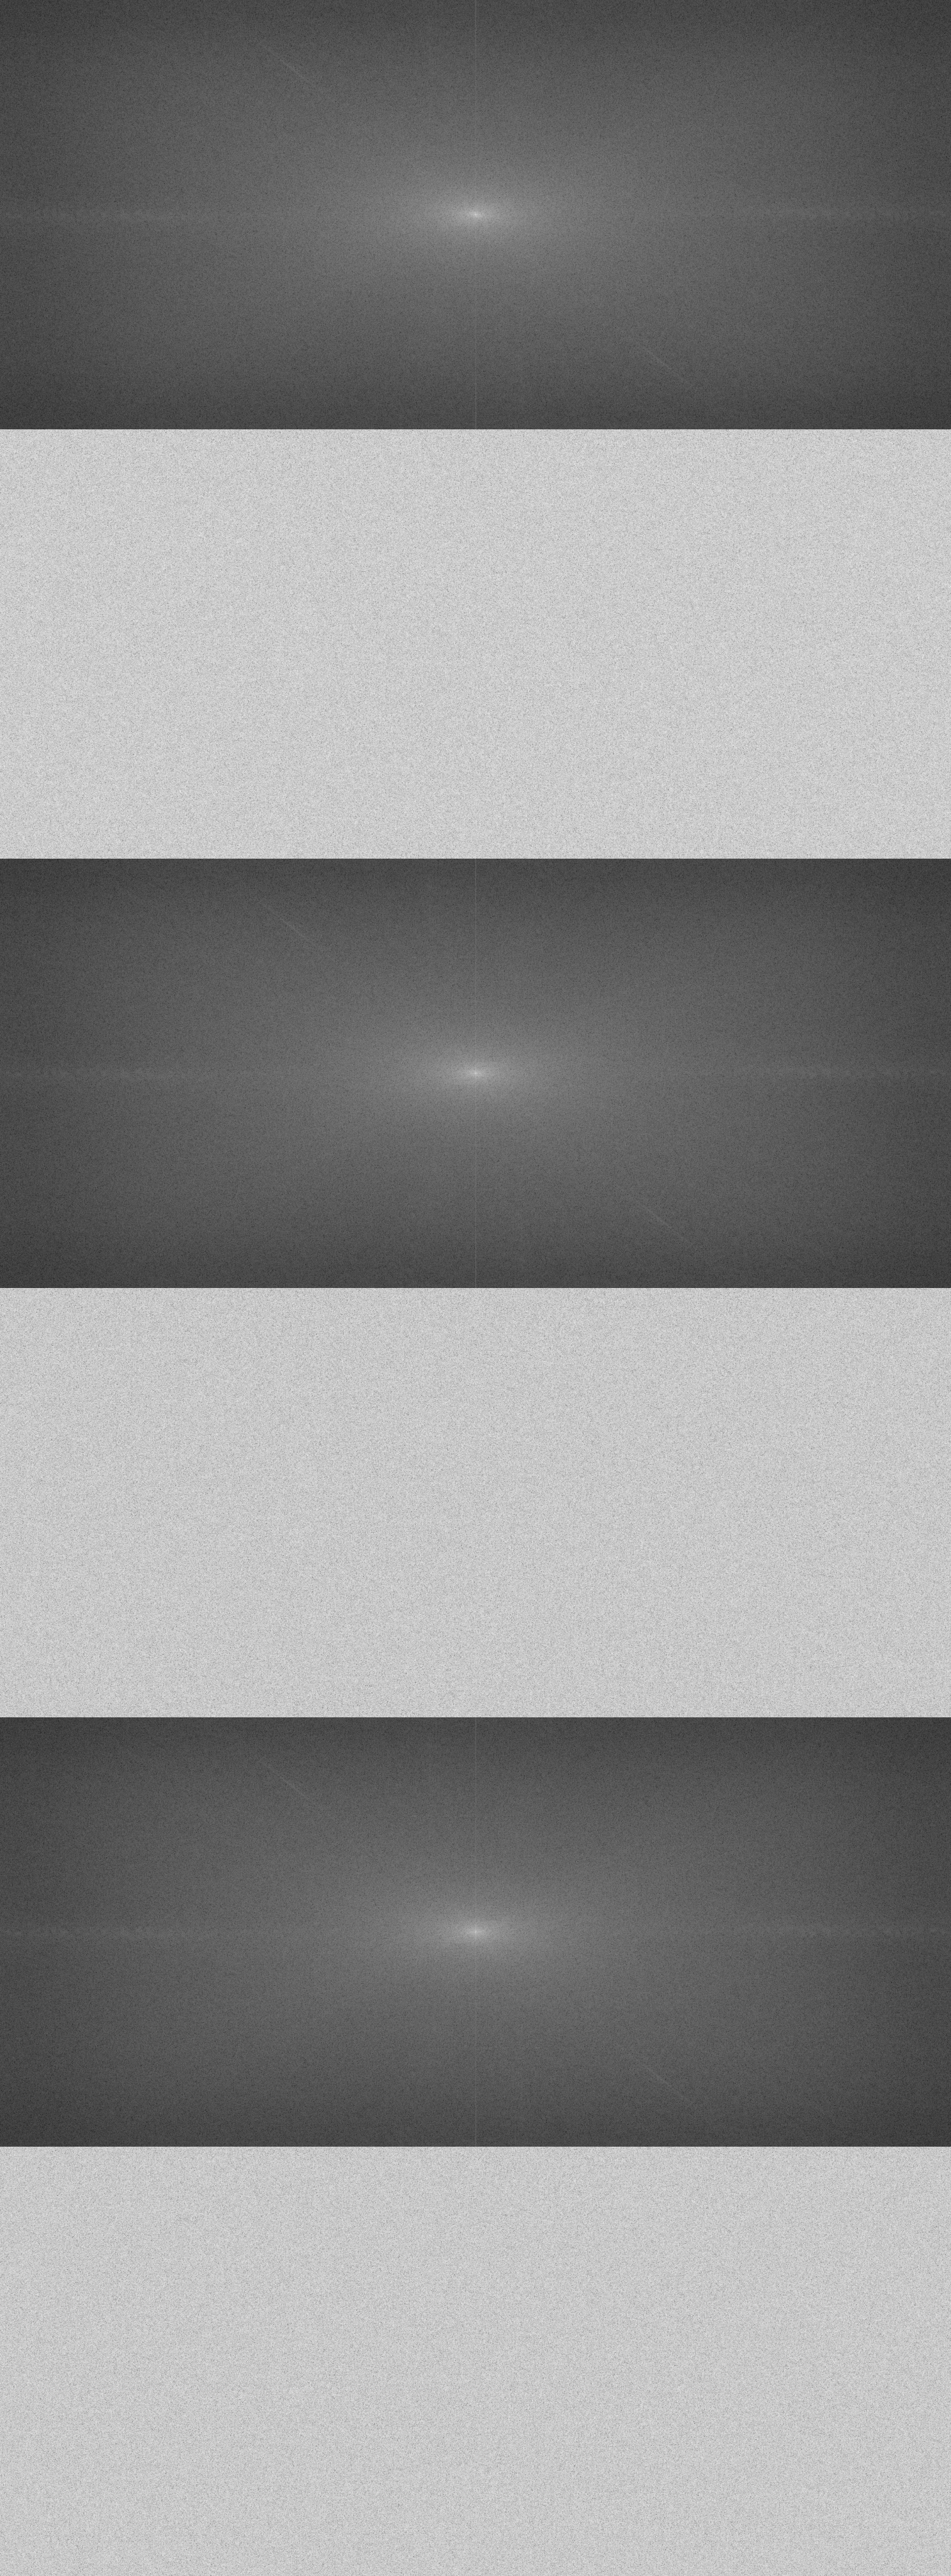
\includegraphics[width=1.0\textwidth,height=65em]{./images/mask_effect/regular_fourier_vs_modulated.png}
    \caption{effect of modulation on fourier visualization}
    \label{fig:modulation_effect}
  \end{figure}
  % \clearpage % End the page
}
\afterpage{%
  % \clearpage % Start a new page
  \thispagestyle{empty} % No header/footer on this page
  \begin{figure}[!htbp]
    \centering
	\captionsetup{justification=centering}
    \includegraphics[width=1.0\textwidth,height=65em]{./images/coded_diffractions_measurements_sat_phone/measurements.png}
    \caption{Measurements on DC\textregistered\space Universe Characters Due to a Random Modulation Plate from Top to Buttom: 
    Red Channel, Green Channel, Blue Channel, and Full RGB}
    \label{fig:coded_diffractions_measurements_dc}
  \end{figure}
  % \clearpage % End the page
}
\afterpage{%
  % \clearpage % Start a new page
  \thispagestyle{empty} % No header/footer on this pages
  \begin{figure}[!htbp]
    \centering
	\captionsetup{justification=centering}
    \includegraphics[width=1.0\textwidth,height=65em]{./images/coded_diffractions_measurements_zoomed_sat_phone/measurements.png}
    \caption{Measurements on DC\textregistered\space Universe Characters Due to a Random Modulation Plate from Top to Buttom: 
    Red Channel, Green Channel, Blue Channel, and Full RGB Zoomed Version}
    % \label{fig:coded_diffractions_measurements_zoomed_dc}
  \end{figure}
  % \clearpage % End the page
}
%%%%%%%%%%%%%%%%%%%%%%%%%%%%%%%%%%%%%%%%%%%%%%%%%%%%%%%%%%%%%
%%%% WF Variants Error During Retrieval Reconstruction %%%%%%
%%%%%%%%%%%%%%%%%%%%%%%%%%%%%%%%%%%%%%%%%%%%%%%%%%%%%%%%%%%%%
\afterpage{%
  % \clearpage % Start a new page
    
    \begin{figure}[!htbp]
      \centering
    \captionsetup{justification=centering}
    % \begin{turn}{-90}
      % This file was created with tikzplotlib v0.10.1.
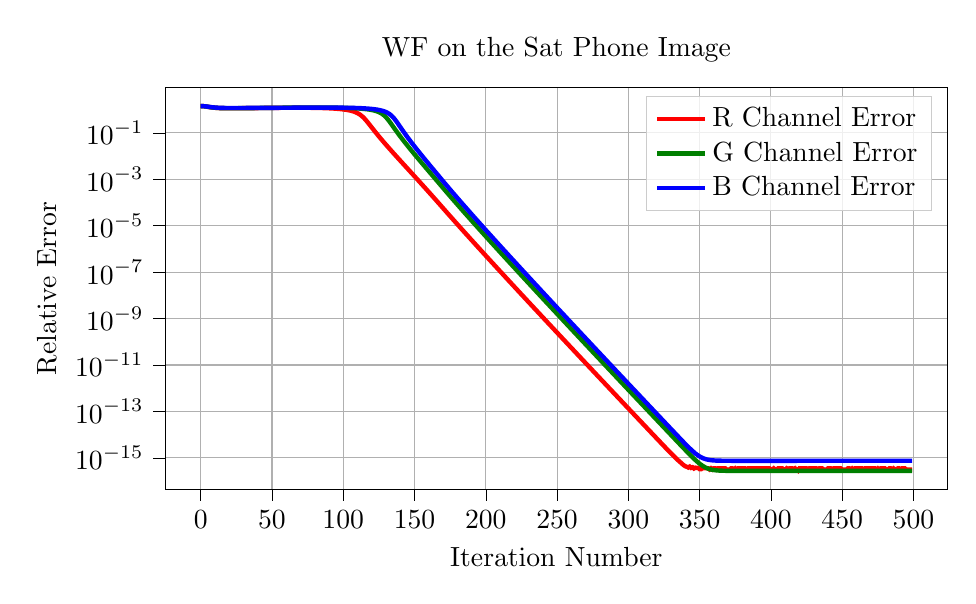
\begin{tikzpicture}

  \definecolor{darkgray176}{RGB}{176,176,176}
  \definecolor{green01270}{RGB}{0,127,0}
  \definecolor{lightgray204}{RGB}{204,204,204}
  
  \begin{axis}[
    width = 0.95\textwidth,
    height = 19em,
  legend cell align={left},
  legend style={fill opacity=0.8, draw opacity=1, text opacity=1, draw=lightgray204},
  log basis y={10},
  tick align=outside,
  tick pos=left,
  title={\ac{WF} on the Sat Phone Image},
  x grid style={darkgray176},
  xlabel={Iteration Number},
  xmajorgrids,
  xmin=-24.95, xmax=523.95,
  xtick style={color=black},
  y grid style={darkgray176},
  ylabel={Relative Error},
  ymajorgrids,
  ymin=4.4579991979902e-17, ymax=8.63401697443202,
  ymode=log,
  ytick style={color=black},
  ytick={1e-19,1e-17,1e-15,1e-13,1e-11,1e-09,1e-07,1e-05,0.001,0.1,10,1000},
  yticklabels={
    \(\displaystyle {10^{-19}}\),
    \(\displaystyle {10^{-17}}\),
    \(\displaystyle {10^{-15}}\),
    \(\displaystyle {10^{-13}}\),
    \(\displaystyle {10^{-11}}\),
    \(\displaystyle {10^{-9}}\),
    \(\displaystyle {10^{-7}}\),
    \(\displaystyle {10^{-5}}\),
    \(\displaystyle {10^{-3}}\),
    \(\displaystyle {10^{-1}}\),
    \(\displaystyle {10^{1}}\),
    \(\displaystyle {10^{3}}\)
  }
  ]
  \addplot [ultra thick, red]
  table {%
  0 1.41304083229291
  1 1.41304083229291
  2 1.40075053191829
  3 1.37810875984083
  4 1.34898985192224
  5 1.31762837115872
  6 1.2873089231327
  7 1.25993548481865
  8 1.23626543024484
  9 1.21634351321272
  10 1.19986245876309
  11 1.18638717598716
  12 1.17547102584549
  13 1.16670648467722
  14 1.15974138182594
  15 1.15427910221536
  16 1.15007241214461
  17 1.14691557348639
  18 1.14463680394046
  19 1.14309185636138
  20 1.14215888731607
  21 1.14173451785236
  22 1.14173088302325
  23 1.1420734371354
  24 1.1426992906485
  25 1.14355588480502
  26 1.14459985233303
  27 1.14579596015269
  28 1.14711607649418
  29 1.14853814434981
  30 1.1500451715524
  31 1.15162426334905
  32 1.15326572714405
  33 1.15496227413647
  34 1.15670833277714
  35 1.15849947799674
  36 1.16033197071268
  37 1.16220239566178
  38 1.16410738245513
  39 1.16604339445817
  40 1.1680065718213
  41 1.16999261781247
  42 1.17199672074407
  43 1.17401350666368
  44 1.1760370202222
  45 1.17806073255321
  46 1.18007757553391
  47 1.18208000149526
  48 1.18406006643146
  49 1.18600953322839
  50 1.18791998965427
  51 1.1897829741486
  52 1.19159010113486
  53 1.19333317696014
  54 1.19500429782813
  55 1.19659592230134
  56 1.19810091300007
  57 1.19951254476822
  58 1.2008244794524
  59 1.20203071016226
  60 1.2031254801034
  61 1.20410318256068
  62 1.20495824926227
  63 1.20568503421231
  64 1.20627769928928
  65 1.20673010667503
  66 1.20703572172282
  67 1.20718752838502
  68 1.20717795794242
  69 1.20699883059521
  70 1.20664130852623
  71 1.20609585832759
  72 1.20535222016756
  73 1.20439938072698
  74 1.20322554671419
  75 1.20181811563659
  76 1.20016364043279
  77 1.19824778452262
  78 1.19605526378799
  79 1.19356977192959
  80 1.19077388552713
  81 1.18764894493531
  82 1.18417490683984
  83 1.1803301638423
  84 1.17609132579283
  85 1.17143295669884
  86 1.16632725984562
  87 1.16074370220597
  88 1.15464856721103
  89 1.14800442241376
  90 1.14076948539276
  91 1.13289686730088
  92 1.12433366863267
  93 1.11501989595195
  94 1.1048871614127
  95 1.09385711896884
  96 1.08183958249966
  97 1.06873026249489
  98 1.05440805126721
  99 1.03873178559376
  100 1.0215364273919
  101 1.00262864085083
  102 0.981781832566269
  103 0.958730902417577
  104 0.933167300459165
  105 0.904735619106213
  106 0.873034053407515
  107 0.837622877030769
  108 0.798047824901299
  109 0.753888831664665
  110 0.704847705116991
  111 0.650887073043263
  112 0.592418870541447
  113 0.530502343709344
  114 0.466948861386335
  115 0.4041864066028
  116 0.34480568850887
  117 0.290933645596429
  118 0.243776113572834
  119 0.203569236148213
  120 0.169857861147062
  121 0.141847606437789
  122 0.118662467418616
  123 0.0994815690337311
  124 0.0835923160166789
  125 0.0703994953766451
  126 0.0594154152975068
  127 0.0502439622781651
  128 0.0425643230886926
  129 0.0361165464845666
  130 0.0306895028024646
  131 0.0261111404838776
  132 0.0222407160427902
  133 0.0189626368978077
  134 0.0161815899204294
  135 0.0138186824117765
  136 0.011808376155005
  137 0.0100960420484357
  138 0.00863600104691611
  139 0.00738994733712528
  140 0.00632567313417344
  141 0.00541603256193314
  142 0.00463809595671639
  143 0.003972456584228
  144 0.00340265994674102
  145 0.00291473216922485
  146 0.0024967888375334
  147 0.00213870945782139
  148 0.00183186567030675
  149 0.00156889367593996
  150 0.00134350316802024
  151 0.00115031651353497
  152 0.000984733085695056
  153 0.000842814574554507
  154 0.000721187846457657
  155 0.000616962523697337
  156 0.000527660942898761
  157 0.000451158547389282
  158 0.000385633093253548
  159 0.000329521315111965
  160 0.00028148191710769
  161 0.000240363936031552
  162 0.000205179674033551
  163 0.00017508152362465
  164 0.000149342112211203
  165 0.000127337280894241
  166 0.000108531485677211
  167 9.24652709738861e-05
  168 7.8744517363141e-05
  169 6.70312095139732e-05
  170 5.70548711295581e-05
  171 4.85802065157934e-05
  172 4.13781190329865e-05
  173 3.52550262416973e-05
  174 3.00472492260453e-05
  175 2.56163083605331e-05
  176 2.18449751922295e-05
  177 1.86339558091995e-05
  178 1.58991022166942e-05
  179 1.35690656821787e-05
  180 1.158332041457e-05
  181 9.89049785973078e-06
  182 8.44698176870462e-06
  183 7.21572238874515e-06
  184 6.16523493624694e-06
  185 5.26875317601607e-06
  186 4.50351365149676e-06
  187 3.85015004764644e-06
  188 3.29218045607382e-06
  189 2.81557306053788e-06
  190 2.40837806118231e-06
  191 2.06041558266109e-06
  192 1.76301092692029e-06
  193 1.50876988725513e-06
  194 1.29138797915754e-06
  195 1.10548840084549e-06
  196 9.46484341815204e-07
  197 8.10461935962089e-07
  198 6.94080727181105e-07
  199 5.94488997124418e-07
  200 5.09251711280877e-07
  201 4.36289182698656e-07
  202 3.73824842539315e-07
  203 3.20340751719174e-07
  204 2.74539695088938e-07
  205 2.35312874993703e-07
  206 2.0171236948809e-07
  207 1.7292764627279e-07
  208 1.48265529962009e-07
  209 1.27133110689783e-07
  210 1.09023158675421e-07
  211 9.35016744558261e-08
  212 8.01972596678691e-08
  213 6.87920402075482e-08
  214 5.90139134079466e-08
  215 5.06299247581681e-08
  216 4.34406084894388e-08
  217 3.72751508324364e-08
  218 3.19872555956319e-08
  219 2.74516094550195e-08
  220 2.35608594400012e-08
  221 2.02230279553505e-08
  222 1.73593016482014e-08
  223 1.4902139752193e-08
  224 1.27936554922161e-08
  225 1.09842309443163e-08
  226 9.43133148473571e-09
  227 8.09849094394214e-09
  228 6.95444275514816e-09
  229 5.97237600794628e-09
  230 5.12929835012235e-09
  231 4.40549034494326e-09
  232 3.78403808003473e-09
  233 3.25043277066857e-09
  234 2.7922277032065e-09
  235 2.39874428685022e-09
  236 2.06082014506671e-09
  237 1.77059321879213e-09
  238 1.52131670883962e-09
  239 1.30720043680268e-09
  240 1.12327484776605e-09
  241 9.65274396483175e-10
  242 8.295375607087e-10
  243 7.12921092688742e-10
  244 6.12726478175975e-10
  245 5.26636859571314e-10
  246 4.52662930925017e-10
  247 3.89096522726149e-10
  248 3.34470778781948e-10
  249 2.87525990882748e-10
  250 2.47180281384653e-10
  251 2.12504446622576e-10
  252 1.82700364659603e-10
  253 1.57082466939422e-10
  254 1.35061834363574e-10
  255 1.16132542181302e-10
  256 9.98599444203135e-11
  257 8.58706086442962e-11
  258 7.3843683695676e-11
  259 6.35034781480233e-11
  260 5.4613093357839e-11
  261 4.69689564796717e-11
  262 4.03961242800164e-11
  263 3.47442476853734e-11
  264 2.98841100986086e-11
  265 2.57046536176947e-11
  266 2.21104192706088e-11
  267 1.90193548917292e-11
  268 1.6360929786004e-11
  269 1.40745137717811e-11
  270 1.21079835559239e-11
  271 1.04165310102656e-11
  272 8.96163028252886e-12
  273 7.71016062490424e-12
  274 6.63364340835764e-12
  275 5.70759288730585e-12
  276 4.91095330989687e-12
  277 4.22562053029913e-12
  278 3.6360244490136e-12
  279 3.12877703190493e-12
  280 2.69236409384488e-12
  281 2.3168836317139e-12
  282 1.99381902522586e-12
  283 1.71584529202883e-12
  284 1.47666265590685e-12
  285 1.27085249272692e-12
  286 1.09375362820568e-12
  287 9.413567736342e-13
  288 8.1021287801406e-13
  289 6.97355920995798e-13
  290 6.00232357613874e-13
  291 5.16647731012772e-13
  292 4.44712585470918e-13
  293 3.82801392040198e-13
  294 3.29516841229749e-13
  295 2.83655483196169e-13
  296 2.44182119102544e-13
  297 2.10206445093937e-13
  298 1.80961815901695e-13
  299 1.55789188428882e-13
  300 1.34120765170605e-13
  301 1.1546846388852e-13
  302 9.94122265851957e-14
  303 8.55903654104743e-14
  304 7.36917771340264e-14
  305 6.3448463114907e-14
  306 5.46302152693448e-14
  307 4.7038302473599e-14
  308 4.05023596643627e-14
  309 3.48751395386313e-14
  310 3.00303682336352e-14
  311 2.58590327314658e-14
  312 2.22675757212162e-14
  313 1.91770277235236e-14
  314 1.6514539688852e-14
  315 1.42205733175583e-14
  316 1.22468592269434e-14
  317 1.05474036792896e-14
  318 9.08406118497216e-15
  319 7.82410699440118e-15
  320 6.74135862387508e-15
  321 5.80745974888677e-15
  322 5.00361104747398e-15
  323 4.31147839653488e-15
  324 3.71298368291181e-15
  325 3.20020227821162e-15
  326 2.7622150814123e-15
  327 2.38278000800833e-15
  328 2.0526930212397e-15
  329 1.78005960675209e-15
  330 1.5359081266963e-15
  331 1.33466690723205e-15
  332 1.15893622943697e-15
  333 1.00880724580487e-15
  334 8.73414478119083e-16
  335 7.72834973260837e-16
  336 6.81427354492899e-16
  337 6.04960154180246e-16
  338 5.28193125442102e-16
  339 4.73848019678606e-16
  340 4.29152053208584e-16
  341 4.09949146712396e-16
  342 3.81558730052092e-16
  343 4.17050609767235e-16
  344 3.68142804314846e-16
  345 3.90106831934385e-16
  346 3.45420433232068e-16
  347 3.74291504797392e-16
  348 3.68946916664764e-16
  349 3.65052696811023e-16
  350 3.24106586888452e-16
  351 3.21456669650585e-16
  352 3.57709402999039e-16
  353 3.56293883365316e-16
  354 3.55294662878602e-16
  355 3.54478989990782e-16
  356 3.53891648251696e-16
  357 3.14559823792432e-16
  358 3.53030889223012e-16
  359 3.13873879139354e-16
  360 3.52482126623621e-16
  361 3.52357404581665e-16
  362 3.13262942160889e-16
  363 3.52076943471237e-16
  364 3.51910811491979e-16
  365 3.51787933554333e-16
  366 3.51646774385229e-16
  367 3.51649834025418e-16
  368 3.51557023546473e-16
  369 3.12452221598899e-16
  370 3.1239464154108e-16
  371 3.12348072958623e-16
  372 3.51255836304449e-16
  373 3.51332114556744e-16
  374 3.12266406964762e-16
  375 3.51137319986342e-16
  376 3.12131185473055e-16
  377 3.5103349717826e-16
  378 3.51114693394955e-16
  379 3.51057502693295e-16
  380 3.51043791792668e-16
  381 3.51055552999738e-16
  382 3.51064933209735e-16
  383 3.12114054546484e-16
  384 3.51003273105356e-16
  385 3.51017528672395e-16
  386 3.50829159783649e-16
  387 3.50860638644281e-16
  388 3.50923243623005e-16
  389 3.50861252091351e-16
  390 3.50854690726162e-16
  391 3.50886964872742e-16
  392 3.50861496358964e-16
  393 3.50801416353633e-16
  394 3.50933502530151e-16
  395 3.50973549260165e-16
  396 3.50923846406392e-16
  397 3.50897278751483e-16
  398 3.50807868829536e-16
  399 3.50633103278778e-16
  400 3.11726202344884e-16
  401 3.11778352458481e-16
  402 3.50609421849605e-16
  403 3.11667947927462e-16
  404 3.11537744834994e-16
  405 3.50579992651914e-16
  406 3.50556340053569e-16
  407 3.50677007384822e-16
  408 3.50569155274989e-16
  409 3.11692284295758e-16
  410 3.11822906938441e-16
  411 3.50527902854085e-16
  412 3.11578118176426e-16
  413 3.50531287021431e-16
  414 3.50456167257061e-16
  415 3.50561622938709e-16
  416 3.11694843758319e-16
  417 3.5058282937597e-16
  418 3.11622969727899e-16
  419 2.79921723112395e-16
  420 3.50607679692845e-16
  421 3.50565657417399e-16
  422 3.50524689509311e-16
  423 3.50530410946712e-16
  424 3.50499160901101e-16
  425 3.50528487998633e-16
  426 3.11572952032304e-16
  427 3.50499412033507e-16
  428 3.50545312467776e-16
  429 3.50498082310753e-16
  430 3.50440446923362e-16
  431 3.50536756966814e-16
  432 3.50380073047591e-16
  433 3.1146265742169e-16
  434 3.5038667003312e-16
  435 3.50383062324251e-16
  436 3.50414862354094e-16
  437 3.11602054815033e-16
  438 3.11526707538431e-16
  439 3.1140156026337e-16
  440 3.50235516669374e-16
  441 3.50168050761011e-16
  442 3.50145525773637e-16
  443 3.11271257621698e-16
  444 3.50136676222177e-16
  445 3.5008571745027e-16
  446 3.50131979958851e-16
  447 3.50074686081073e-16
  448 3.50073392062209e-16
  449 3.50027502349744e-16
  450 3.11204625463241e-16
  451 3.11097661084213e-16
  452 3.11159821531887e-16
  453 3.10913669109371e-16
  454 3.49874351226878e-16
  455 3.50002349140267e-16
  456 3.11205620148763e-16
  457 3.50050939855119e-16
  458 3.11221955785715e-16
  459 3.50055870333167e-16
  460 3.50054371845359e-16
  461 3.49988723800055e-16
  462 3.4995266477459e-16
  463 3.50008307294323e-16
  464 3.49899387794213e-16
  465 3.10924114593898e-16
  466 3.49994945546622e-16
  467 3.49946753627546e-16
  468 3.49839962447426e-16
  469 3.49884439788185e-16
  470 3.49834885827957e-16
  471 3.49803420487876e-16
  472 3.49780838518247e-16
  473 3.49760408047225e-16
  474 3.10972716060404e-16
  475 3.49762431790602e-16
  476 3.1102211467364e-16
  477 3.49807768263771e-16
  478 3.49779172727577e-16
  479 3.49846137260365e-16
  480 3.49918609919361e-16
  481 3.11102564154487e-16
  482 3.11013402775254e-16
  483 3.49832918876628e-16
  484 3.49949493472246e-16
  485 3.10948580181399e-16
  486 3.49865627022087e-16
  487 3.10972892389382e-16
  488 3.10993911606857e-16
  489 3.49840747633624e-16
  490 3.49959122396625e-16
  491 3.11015918210851e-16
  492 3.49948572490931e-16
  493 3.4992171577549e-16
  494 3.50042373390814e-16
  495 3.11071392102884e-16
  496 3.11065250997472e-16
  497 3.11053362257692e-16
  498 3.10948578529639e-16
  499 3.1101733687535e-16
  };
  \addlegendentry{R Channel Error}
  \addplot [ultra thick, green01270]
  table {%
  0 1.41369012762637
  1 1.41369012762637
  2 1.40189058697223
  3 1.38008735352619
  4 1.35189391902826
  5 1.32131690508181
  6 1.2915352465448
  7 1.26445633682881
  8 1.24089344959986
  9 1.22095515841556
  10 1.20438604303676
  11 1.19078701405053
  12 1.17973413261726
  13 1.17083313865511
  14 1.16373899545422
  15 1.15815847110104
  16 1.15384554844616
  17 1.15059455660312
  18 1.14823327457355
  19 1.14661691509695
  20 1.14562324507033
  21 1.14514879736654
  22 1.14510600060363
  23 1.14542101114642
  24 1.14603203404688
  25 1.14688794703268
  26 1.14794708310148
  27 1.14917607463395
  28 1.15054870791351
  29 1.15204477535508
  30 1.15364893952487
  31 1.15534963694848
  32 1.15713805230229
  33 1.15900718835296
  34 1.16095104815529
  35 1.16296393729633
  36 1.16503988792608
  37 1.16717220398434
  38 1.1693531280685
  39 1.17157363338439
  40 1.17382334715768
  41 1.1760906125883
  42 1.17836269307522
  43 1.18062611405383
  44 1.18286712471146
  45 1.18507224599452
  46 1.18722885604545
  47 1.18932575362388
  48 1.19135363789002
  49 1.19330545115799
  50 1.19517654919401
  51 1.19696468791365
  52 1.19866984067847
  53 1.20029388137805
  54 1.20184018117662
  55 1.20331316979316
  56 1.20471790661661
  57 1.20605969573223
  58 1.20734376551484
  59 1.20857502081154
  60 1.20975786579638
  61 1.21089608906815
  62 1.2119927992984
  63 1.21305039901369
  64 1.21407058504301
  65 1.2150543659865
  66 1.21600208917023
  67 1.21691347156617
  68 1.2177876308801
  69 1.21862311437846
  70 1.21941792404804
  71 1.22016953740984
  72 1.22087492380206
  73 1.22153055626518
  74 1.22213241935507
  75 1.22267601331578
  76 1.22315635509065
  77 1.22356797665731
  78 1.2239049211508
  79 1.2241607371959
  80 1.22432847180821
  81 1.22440066214344
  82 1.22436932627573
  83 1.22422595306758
  84 1.22396149105467
  85 1.22356633610896
  86 1.22303031746226
  87 1.22234268147155
  88 1.22149207228862
  89 1.22046650836177
  90 1.21925335344936
  91 1.21783928056515
  92 1.21621022700446
  93 1.21435133831527
  94 1.21224689877489
  95 1.20988024559949
  96 1.2072336637352
  97 1.20428825763344
  98 1.20102379586911
  99 1.19741852378057
  100 1.19344893844562
  101 1.18908951919974
  102 1.184312405476
  103 1.17908701191059
  104 1.1733795682993
  105 1.16715256896922
  106 1.16036411226984
  107 1.15296710597375
  108 1.14490830814483
  109 1.13612716516987
  110 1.12655439880883
  111 1.11611028195107
  112 1.10470252801388
  113 1.0922237016224
  114 1.07854803911239
  115 1.06352754877127
  116 1.04698724797982
  117 1.02871939911265
  118 1.00847665166237
  119 0.985964130372013
  120 0.960830814797442
  121 0.932661192823218
  122 0.900969414383116
  123 0.865200463714724
  124 0.824746811733807
  125 0.778995109769506
  126 0.727425124249443
  127 0.669787794579665
  128 0.606377569235692
  129 0.538360518993716
  130 0.468005064984124
  131 0.398544081339804
  132 0.333477810434682
  133 0.27555769884199
  134 0.226102929093053
  135 0.185057645178012
  136 0.151531714510041
  137 0.124339063235004
  138 0.102316581131928
  139 0.0844540938664771
  140 0.0699218499754252
  141 0.0580556306179678
  142 0.0483293650547611
  143 0.040327539727351
  144 0.03372148761359
  145 0.0282502917821106
  146 0.0237058486050203
  147 0.0199213309876637
  148 0.0167623129622795
  149 0.0141199364561389
  150 0.0119056323524884
  151 0.0100470224062079
  152 0.00848471995725654
  153 0.00716981746508688
  154 0.00606190159152758
  155 0.0051274758506525
  156 0.00433870005575109
  157 0.00367237753042415
  158 0.00310913727534084
  159 0.00263277044602202
  160 0.00222968966458075
  161 0.00188848663758969
  162 0.00159956885171251
  163 0.00135486018489785
  164 0.00114755340993152
  165 0.000971905005038632
  166 0.000823064590794296
  167 0.000696932809035517
  168 0.000590042641714973
  169 0.000499460106610363
  170 0.000422849653411491
  171 0.00035820452865753
  172 0.000303614775256166
  173 0.000257483393238809
  174 0.000218473435888206
  175 0.000185464383494355
  176 0.000157516097090254
  177 0.000133838980469468
  178 0.000113769238753661
  179 9.6748329890056e-05
  180 8.23058726449836e-05
  181 7.00454094067851e-05
  182 5.96325310476792e-05
  183 5.07849594169401e-05
  184 4.32642548409259e-05
  185 3.68688745271192e-05
  186 3.14283555800156e-05
  187 2.67984354843981e-05
  188 2.28569550340218e-05
  189 1.95004150942064e-05
  190 1.66410803421722e-05
  191 1.42045410813307e-05
  192 1.21276590652705e-05
  193 1.03568355529536e-05
  194 8.84655000360615e-06
  195 7.55812627879315e-06
  196 6.45869025253856e-06
  197 5.52028858636975e-06
  198 4.71914330754616e-06
  199 4.03502090272139e-06
  200 3.4506980430758e-06
  201 2.95150890390122e-06
  202 2.52496142522448e-06
  203 2.16041185763305e-06
  204 1.84878861312182e-06
  205 1.58235784762082e-06
  206 1.35452438401099e-06
  207 1.15966257858165e-06
  208 9.92972570586076e-07
  209 8.5035805925098e-07
  210 7.28322346549918e-07
  211 6.23879885007711e-07
  212 5.34480992586441e-07
  213 4.57947753755083e-07
  214 3.92419427546455e-07
  215 3.36305938502448e-07
  216 2.88248242204913e-07
  217 2.47084539750063e-07
  218 2.11821470208426e-07
  219 1.81609541171795e-07
  220 1.55722168588655e-07
  221 1.33537791302762e-07
  222 1.14524605653455e-07
  223 9.82275333412872e-08
  224 8.42570933853692e-08
  225 7.22798979352338e-08
  226 6.20105333010765e-08
  227 5.32046229162766e-08
  228 4.56528990228553e-08
  229 3.91761354490527e-08
  230 3.36208156136106e-08
  231 2.88554284289434e-08
  232 2.47673005485515e-08
  233 2.12598868492455e-08
  234 1.82504524893133e-08
  235 1.56680896413569e-08
  236 1.34520203220836e-08
  237 1.15501438347472e-08
  238 9.91779338855345e-09
  239 8.51667162803122e-09
  240 7.31393920236851e-09
  241 6.28143427328488e-09
  242 5.39500406203243e-09
  243 4.63393228463527e-09
  244 3.98044865812363e-09
  245 3.41930866779043e-09
  246 2.93743348651968e-09
  247 2.52360140473893e-09
  248 2.16818337180421e-09
  249 1.86291631885224e-09
  250 1.60070884735762e-09
  251 1.37547464399881e-09
  252 1.18198965149463e-09
  253 1.01576959729701e-09
  254 8.72964967460485e-10
  255 7.50270933914663e-10
  256 6.44850097342268e-10
  257 5.54266219161625e-10
  258 4.7642737205944e-10
  259 4.09537168582144e-10
  260 3.52052915624189e-10
  261 3.02649707638212e-10
  262 2.60189616071177e-10
  263 2.23695246371252e-10
  264 1.92327043426134e-10
  265 1.65363814322753e-10
  266 1.42186007899713e-10
  267 1.22261361725891e-10
  268 1.05132580901597e-10
  269 9.0406759288475e-11
  270 7.77462963356213e-11
  271 6.68610990223296e-11
  272 5.75018837851802e-11
  273 4.94544262152222e-11
  274 4.25346213690437e-11
  275 3.65842429028297e-11
  276 3.14672980469155e-11
  277 2.70668996326482e-11
  278 2.32825771211669e-11
  279 2.00279669816893e-11
  280 1.72288293854708e-11
  281 1.48213436880689e-11
  282 1.2750643422336e-11
  283 1.09695588187485e-11
  284 9.43753525680741e-12
  285 8.1197041835673e-12
  286 6.98608482865329e-12
  287 6.01089813556958e-12
  288 5.17197702181164e-12
  289 4.45025946289229e-12
  290 3.82935383954527e-12
  291 3.29516294495349e-12
  292 2.83556381232556e-12
  293 2.44012939641398e-12
  294 2.09989284050769e-12
  295 1.80714109473656e-12
  296 1.55524055020991e-12
  297 1.33848491974641e-12
  298 1.15196591870301e-12
  299 9.91461763166889e-13
  300 8.53340562091733e-13
  301 7.34477757504331e-13
  302 6.321857496281e-13
  303 5.44152283900738e-13
  304 4.68388053033393e-13
  305 4.03181474390616e-13
  306 3.47060186094937e-13
  307 2.98756885329753e-13
  308 2.57181904548131e-13
  309 2.21396953647392e-13
  310 1.90595302148351e-13
  311 1.64082192448554e-13
  312 1.41259890531576e-13
  313 1.2161457935667e-13
  314 1.04703331547893e-13
  315 9.01455732084903e-14
  316 7.76135013161696e-14
  317 6.68247767878021e-14
  318 5.75368905024239e-14
  319 4.9540856350346e-14
  320 4.26569859386225e-14
  321 3.67302753848782e-14
  322 3.16276940164812e-14
  323 2.72344885668249e-14
  324 2.34520793648012e-14
  325 2.01954759363211e-14
  326 1.73914750809762e-14
  327 1.49771424024555e-14
  328 1.2898475107389e-14
  329 1.11086316093717e-14
  330 9.56761602371644e-15
  331 8.24077352576644e-15
  332 7.09855908476508e-15
  333 6.11500813882769e-15
  334 5.26831517550235e-15
  335 4.53948266372921e-15
  336 3.91226438493936e-15
  337 3.3724757845496e-15
  338 2.9081031164123e-15
  339 2.50881082639924e-15
  340 2.16543113370476e-15
  341 1.87050640301918e-15
  342 1.61729392523711e-15
  343 1.4002348149751e-15
  344 1.21436882958075e-15
  345 1.05559675856197e-15
  346 9.20344176220242e-16
  347 8.05290649778465e-16
  348 7.08136440254482e-16
  349 6.26422071604253e-16
  350 5.58009250510861e-16
  351 5.01163978901607e-16
  352 4.54325819437521e-16
  353 4.16116015194898e-16
  354 3.85346240187478e-16
  355 3.60461363794259e-16
  356 3.40748113133214e-16
  357 3.25225478094756e-16
  358 3.13055210747577e-16
  359 3.03756323679584e-16
  360 2.96532986334334e-16
  361 2.90873714434146e-16
  362 2.86711660121462e-16
  363 2.83553247974908e-16
  364 2.80981859881312e-16
  365 2.79093537523105e-16
  366 2.77730681088721e-16
  367 2.7665698805977e-16
  368 2.75756016255335e-16
  369 2.75018269235004e-16
  370 2.7462616115758e-16
  371 2.74312969733145e-16
  372 2.73886817603015e-16
  373 2.73517742509063e-16
  374 2.73379246229763e-16
  375 2.73325679623975e-16
  376 2.73269639432264e-16
  377 2.73143826668914e-16
  378 2.72990060156971e-16
  379 2.7288331976958e-16
  380 2.72734865003658e-16
  381 2.72806195506596e-16
  382 2.72653607889796e-16
  383 2.72575063891364e-16
  384 2.72559006710989e-16
  385 2.72518547118313e-16
  386 2.72522182999737e-16
  387 2.72582591053251e-16
  388 2.72445345448243e-16
  389 2.72499229997346e-16
  390 2.72457452992589e-16
  391 2.72450862956145e-16
  392 2.7256066609889e-16
  393 2.72531341882094e-16
  394 2.72497173784597e-16
  395 2.72445572504668e-16
  396 2.72443267968055e-16
  397 2.72419154113713e-16
  398 2.72481339132564e-16
  399 2.72439208448979e-16
  400 2.7228560324762e-16
  401 2.72309082824922e-16
  402 2.72348725928654e-16
  403 2.72459433388637e-16
  404 2.7235995596342e-16
  405 2.72376015063248e-16
  406 2.724295739841e-16
  407 2.72447349932114e-16
  408 2.7248952891331e-16
  409 2.72460304729115e-16
  410 2.72445841910556e-16
  411 2.72415619323416e-16
  412 2.72306356699197e-16
  413 2.7244121834995e-16
  414 2.72573397515295e-16
  415 2.72516215161679e-16
  416 2.72406366060148e-16
  417 2.72294914742081e-16
  418 2.7235595118905e-16
  419 2.72275509413034e-16
  420 2.72278333657968e-16
  421 2.72439608576441e-16
  422 2.72376577037219e-16
  423 2.72296397271047e-16
  424 2.72388486385338e-16
  425 2.72423900782606e-16
  426 2.72439011548193e-16
  427 2.72302862178702e-16
  428 2.7230481244901e-16
  429 2.72217491408669e-16
  430 2.72361142374607e-16
  431 2.72272944178873e-16
  432 2.72471656481958e-16
  433 2.72442289979837e-16
  434 2.72587351950428e-16
  435 2.72510384738185e-16
  436 2.72503311929433e-16
  437 2.72370904625114e-16
  438 2.72407169388514e-16
  439 2.72472052871631e-16
  440 2.7239525345567e-16
  441 2.7240776253965e-16
  442 2.72227640483875e-16
  443 2.72377454420625e-16
  444 2.72401552069596e-16
  445 2.72308694214809e-16
  446 2.72385332959299e-16
  447 2.72274683533633e-16
  448 2.72285206969758e-16
  449 2.72371658356526e-16
  450 2.7241870694625e-16
  451 2.72360399673543e-16
  452 2.72503134540168e-16
  453 2.72435096783387e-16
  454 2.72450744032345e-16
  455 2.72350513697356e-16
  456 2.72483112837778e-16
  457 2.7247891771177e-16
  458 2.72446756486814e-16
  459 2.72345335581299e-16
  460 2.7251524399007e-16
  461 2.72335141676918e-16
  462 2.72480669464577e-16
  463 2.7251793194272e-16
  464 2.72608277471788e-16
  465 2.72498252168013e-16
  466 2.72479008833162e-16
  467 2.72338257800122e-16
  468 2.72423328525434e-16
  469 2.72332936422754e-16
  470 2.72364189129203e-16
  471 2.72336723180472e-16
  472 2.72254983956077e-16
  473 2.72321196714634e-16
  474 2.72231300522217e-16
  475 2.72312592104921e-16
  476 2.72344070625484e-16
  477 2.72425742427392e-16
  478 2.7236242590845e-16
  479 2.72416531141513e-16
  480 2.72415432483224e-16
  481 2.7245294466729e-16
  482 2.72478764003554e-16
  483 2.72383558092558e-16
  484 2.72525896304158e-16
  485 2.7234634338225e-16
  486 2.72471894552512e-16
  487 2.7257668878811e-16
  488 2.72467191388974e-16
  489 2.72454018791717e-16
  490 2.72474013904164e-16
  491 2.72564950589354e-16
  492 2.72406711641349e-16
  493 2.72440726392993e-16
  494 2.72468807238083e-16
  495 2.72551799091851e-16
  496 2.72467419059093e-16
  497 2.72442414892838e-16
  498 2.72446180482295e-16
  499 2.72481406347768e-16
  };
  \addlegendentry{G Channel Error}
  \addplot [ultra thick, blue]
  table {%
  0 1.41395913055666
  1 1.41395913055666
  2 1.40441062990906
  3 1.38657370989164
  4 1.36304297236126
  5 1.33684681629779
  6 1.3105922767176
  7 1.28604627085418
  8 1.26414479333358
  9 1.24521187314483
  10 1.22920140784832
  11 1.21588029299105
  12 1.20494284923904
  13 1.19607321196522
  14 1.18897498815333
  15 1.18338255519575
  16 1.17906302194479
  17 1.17581400063112
  18 1.17345993344334
  19 1.17184833328143
  20 1.17084653366568
  21 1.17033913048395
  22 1.17022608125503
  23 1.17042132087942
  24 1.17085171268179
  25 1.17145615698717
  26 1.17218471215443
  27 1.17299763285057
  28 1.17386428561405
  29 1.17476195160615
  30 1.17567456277574
  31 1.17659143648919
  32 1.17750607545198
  33 1.17841508837884
  34 1.17931726800329
  35 1.18021284226453
  36 1.18110289617238
  37 1.18198894837933
  38 1.18287265858121
  39 1.18375563895531
  40 1.18463934367953
  41 1.18552501374273
  42 1.18641365850436
  43 1.18730605986548
  44 1.1882027888965
  45 1.18910422805134
  46 1.19001059461555
  47 1.19092196284847
  48 1.1918382835101
  49 1.19275940024814
  50 1.19368506278805
  51 1.19461493712026
  52 1.1955486129941
  53 1.19648560906052
  54 1.19742537599384
  55 1.1983672978883
  56 1.19931069218303
  57 1.20025480832591
  58 1.2011988253471
  59 1.20214184847847
  60 1.20308290492492
  61 1.20402093886888
  62 1.20495480576835
  63 1.20588326599123
  64 1.20680497781407
  65 1.20771848980095
  66 1.20862223256723
  67 1.2095145099239
  68 1.21039348939001
  69 1.21125719205388
  70 1.21210348175792
  71 1.21293005357738
  72 1.21373442155946
  73 1.21451390568721
  74 1.21526561803127
  75 1.21598644805246
  76 1.21667304701967
  77 1.21732181150931
  78 1.21792886595581
  79 1.21849004422573
  80 1.21900087019154
  81 1.21945653728353
  82 1.21985188699977
  83 1.22018138635336
  84 1.2204391042327
  85 1.22061868664311
  86 1.22071333078595
  87 1.22071575791252
  88 1.22061818486227
  89 1.22041229415623
  90 1.22008920246336
  91 1.21963942718586
  92 1.21905285081609
  93 1.21831868259813
  94 1.21742541687646
  95 1.21636078732964
  96 1.21511171606231
  97 1.21366425626043
  98 1.21200352679528
  99 1.21011363678565
  100 1.2079775976837
  101 1.20557721992779
  102 1.20289299058764
  103 1.19990392769316
  104 1.196587406058
  105 1.19291894834428
  106 1.18887197381453
  107 1.18441749561098
  108 1.17952375540192
  109 1.17415578172103
  110 1.16827485514528
  111 1.1618378594143
  112 1.15479649243894
  113 1.14709630456873
  114 1.13867552310829
  115 1.12946361144791
  116 1.11937949782279
  117 1.10832939219299
  118 1.0962040898089
  119 1.08287563705724
  120 1.06819321092005
  121 1.05197804255459
  122 1.03401720895174
  123 1.01405614731464
  124 0.991789861136314
  125 0.96685307554506
  126 0.938810233104888
  127 0.907147507708466
  128 0.87127147015297
  129 0.830523420871599
  130 0.784225484571571
  131 0.731784033958566
  132 0.67288325909663
  133 0.607791187247108
  134 0.537740070512055
  135 0.465204151117209
  136 0.393745534250991
  137 0.327192337355956
  138 0.268455651125089
  139 0.218792428072704
  140 0.177961591397852
  141 0.144888520491637
  142 0.118256414439944
  143 0.0968237060413551
  144 0.0795375514658582
  145 0.0655469490835792
  146 0.0541784819256492
  147 0.0449034249649851
  148 0.0373070495713266
  149 0.0310631926105369
  150 0.02591421537632
  151 0.021655552521365
  152 0.0181238997553223
  153 0.0151881955733625
  154 0.0127427190769026
  155 0.0107017832370564
  156 0.00899563178994992
  157 0.0075672473137941
  158 0.00636985259661118
  159 0.00536494263233238
  160 0.00452072531727308
  161 0.00381087896161346
  162 0.00321355695349284
  163 0.00271058642466488
  164 0.00228682010225673
  165 0.00192960980219878
  166 0.00162837703183981
  167 0.00137426150639933
  168 0.00115983247223799
  169 0.000978850881228693
  170 0.000826368672075703
  171 0.000698164673132124
  172 0.000590269501134415
  173 0.000499383787377918
  174 0.000422760707525082
  175 0.000358110040801236
  176 0.000303519608086164
  177 0.000257390784572507
  178 0.000218385445721432
  179 0.000185382227302336
  180 0.000157440393219657
  181 0.00013376993278943
  182 0.000113706770650244
  183 9.66921818033403e-05
  184 8.22556723844137e-05
  185 7.00007222228724e-05
  186 5.95928947214196e-05
  187 5.07499083244201e-05
  188 4.32333359617841e-05
  189 3.68416576169368e-05
  190 3.14044391606614e-05
  191 2.67774498794191e-05
  192 2.28385633546254e-05
  193 1.94843128399312e-05
  194 1.66269940993924e-05
  195 1.41922266678793e-05
  196 1.21168993689111e-05
  197 1.03474382372435e-05
  198 8.83834520004783e-06
  199 7.55096434417043e-06
  200 6.45243964146858e-06
  201 5.51483386836938e-06
  202 4.71438334330364e-06
  203 4.03086718409393e-06
  204 3.4470731945538e-06
  205 2.94834533877865e-06
  206 2.5222001470568e-06
  207 2.15800139604941e-06
  208 1.84668408243177e-06
  209 1.58052011663488e-06
  210 1.35291934582654e-06
  211 1.15826050970299e-06
  212 9.91747569463322e-07
  213 8.49287555148034e-07
  214 7.27386670475806e-07
  215 6.23061895258467e-07
  216 5.3376574822643e-07
  217 4.5732223010328e-07
  218 3.91872268379954e-07
  219 3.35827240361655e-07
  220 2.87829366660215e-07
  221 2.46717950081623e-07
  222 2.11500589302863e-07
  223 1.81328627918638e-07
  224 1.55476210346022e-07
  225 1.33322410350911e-07
  226 1.14335977794378e-07
  227 9.80623170627308e-08
  228 8.41123682107538e-08
  229 7.21531107480478e-08
  230 6.18994516037872e-08
  231 5.31072941179396e-08
  232 4.55676149661018e-08
  233 3.91014014925412e-08
  234 3.35553236787708e-08
  235 2.87980334924991e-08
  236 2.47170001358692e-08
  237 2.121580313847e-08
  238 1.82118166883092e-08
  239 1.56342283501089e-08
  240 1.34223436132898e-08
  241 1.15241348431223e-08
  242 9.89499921189382e-09
  243 8.49669537090772e-09
  244 7.29643302047139e-09
  245 6.26609328223267e-09
  246 5.38156102133598e-09
  247 4.62215292842862e-09
  248 3.97012762073069e-09
  249 3.41026590947278e-09
  250 2.92951116980478e-09
  251 2.51666114820028e-09
  252 2.16210385341548e-09
  253 1.8575911710799e-09
  254 1.59604481728379e-09
  255 1.3713899753069e-09
  256 1.17841266713064e-09
  257 1.01263746064022e-09
  258 8.70222593326503e-10
  259 7.47870032681699e-10
  260 6.42748343237614e-10
  261 5.52426508422315e-10
  262 4.74817186863992e-10
  263 4.08128009827819e-10
  264 3.50819804655569e-10
  265 3.01570759727427e-10
  266 2.5924565177034e-10
  267 2.22869461683029e-10
  268 1.91604716869596e-10
  269 1.64732048529222e-10
  270 1.41633507674322e-10
  271 1.21778230678413e-10
  272 1.04710154409745e-10
  273 9.00374496293597e-11
  274 7.7423457738213e-11
  275 6.65789139002334e-11
  276 5.72552588821099e-11
  277 4.92389021460777e-11
  278 4.23462968625355e-11
  279 3.64197035244435e-11
  280 3.13235534734051e-11
  281 2.69413365908357e-11
  282 2.31729067269217e-11
  283 1.99321865125886e-11
  284 1.71451894521296e-11
  285 1.4748313707999e-11
  286 1.26868827207001e-11
  287 1.09138982445084e-11
  288 9.38894992118695e-12
  289 8.07729828882338e-12
  290 6.94907772880311e-12
  291 5.97860513509108e-12
  292 5.14380040680632e-12
  293 4.4256762591421e-12
  294 3.80790922784773e-12
  295 3.27645744012601e-12
  296 2.81924816224743e-12
  297 2.42590143362758e-12
  298 2.08748585989574e-12
  299 1.79632316248367e-12
  300 1.5458088011637e-12
  301 1.33026276066959e-12
  302 1.14479896592981e-12
  303 9.85215074496e-13
  304 8.47895943683234e-13
  305 7.29732794890678e-13
  306 6.28051951038338e-13
  307 5.40550637868487e-13
  308 4.65250295920873e-13
  309 4.00448163300153e-13
  310 3.44679318041587e-13
  311 2.96683559848742e-13
  312 2.55376248577121e-13
  313 2.19824855580714e-13
  314 1.89226298666967e-13
  315 1.62890369315832e-13
  316 1.40222428000292e-13
  317 1.20711470412104e-13
  318 1.03917387832642e-13
  319 8.94614725318673e-14
  320 7.70180895807784e-14
  321 6.6306761566846e-14
  322 5.70862246368029e-14
  323 4.91488721980871e-14
  324 4.23158572450948e-14
  325 3.64335744801825e-14
  326 3.1369654380324e-14
  327 2.70100644728052e-14
  328 2.32569811157859e-14
  329 2.00257756591306e-14
  330 1.72439485702556e-14
  331 1.48488035436603e-14
  332 1.2787309532331e-14
  333 1.10120563867512e-14
  334 9.48690190570565e-15
  335 8.17669723279949e-15
  336 7.04527764647269e-15
  337 6.07178047399181e-15
  338 5.23422723575769e-15
  339 4.51387693068481e-15
  340 3.89452454531957e-15
  341 3.40101642844054e-15
  342 2.92989948039663e-15
  343 2.56482170109233e-15
  344 2.23660744362303e-15
  345 1.95795023607912e-15
  346 1.74437291759105e-15
  347 1.52453033352647e-15
  348 1.38705792754612e-15
  349 1.25322285841003e-15
  350 1.14391331529049e-15
  351 1.055453721428e-15
  352 9.84733349957467e-16
  353 9.28907558875713e-16
  354 8.85114313300861e-16
  355 8.51035732002271e-16
  356 8.24974980511447e-16
  357 8.04895170670939e-16
  358 7.8963664852626e-16
  359 7.78210134245139e-16
  360 7.69382960122557e-16
  361 7.62888873577688e-16
  362 7.57875541883198e-16
  363 7.54221086911195e-16
  364 7.51300690240396e-16
  365 7.49297464972346e-16
  366 7.47617412815907e-16
  367 7.46557975356999e-16
  368 7.45545555612162e-16
  369 7.4484601144112e-16
  370 7.44352817447754e-16
  371 7.43922079701073e-16
  372 7.43712083900308e-16
  373 7.43349116754733e-16
  374 7.4316752015252e-16
  375 7.43122456458013e-16
  376 7.43091117684945e-16
  377 7.43044169542844e-16
  378 7.42965675541909e-16
  379 7.428300152873e-16
  380 7.42811701832298e-16
  381 7.42893048052438e-16
  382 7.42919085507132e-16
  383 7.42777542374134e-16
  384 7.42837616797672e-16
  385 7.42765468465871e-16
  386 7.42758021563637e-16
  387 7.42830743030003e-16
  388 7.42880683242493e-16
  389 7.42810698651396e-16
  390 7.42749992358062e-16
  391 7.4280122605402e-16
  392 7.4281367706085e-16
  393 7.43005944631645e-16
  394 7.42836705602124e-16
  395 7.43004697646663e-16
  396 7.42994049270727e-16
  397 7.43095264219357e-16
  398 7.43012475421464e-16
  399 7.43126399145454e-16
  400 7.43015605231393e-16
  401 7.43200700334101e-16
  402 7.43149677099462e-16
  403 7.43263265283389e-16
  404 7.43376033866242e-16
  405 7.43355190520371e-16
  406 7.4334215132712e-16
  407 7.43388453533806e-16
  408 7.43524374570234e-16
  409 7.43364832740687e-16
  410 7.43547892530233e-16
  411 7.43440080317899e-16
  412 7.43604136907748e-16
  413 7.43459884572887e-16
  414 7.43603412411551e-16
  415 7.43536887766929e-16
  416 7.43575705787886e-16
  417 7.43584552644797e-16
  418 7.43602085336872e-16
  419 7.43751205046281e-16
  420 7.43666023459474e-16
  421 7.43735876671994e-16
  422 7.43700208350805e-16
  423 7.43755926854133e-16
  424 7.43756001619526e-16
  425 7.43793481347987e-16
  426 7.43654290290197e-16
  427 7.43816121902917e-16
  428 7.43686396317233e-16
  429 7.43889470763018e-16
  430 7.43813474482128e-16
  431 7.43983366011811e-16
  432 7.43850670957579e-16
  433 7.43921070766916e-16
  434 7.43797417535297e-16
  435 7.4397911012166e-16
  436 7.43825426228429e-16
  437 7.43894656755682e-16
  438 7.43884054672139e-16
  439 7.43901515831671e-16
  440 7.43935889239184e-16
  441 7.44025843206469e-16
  442 7.43992556035088e-16
  443 7.44088171943324e-16
  444 7.44087242212277e-16
  445 7.44141366753235e-16
  446 7.44122366998918e-16
  447 7.4413469190814e-16
  448 7.44083771016007e-16
  449 7.44193461090567e-16
  450 7.44158762693386e-16
  451 7.44277019290983e-16
  452 7.44264103348978e-16
  453 7.44352390077065e-16
  454 7.44272318915013e-16
  455 7.4427317058848e-16
  456 7.44343621771753e-16
  457 7.44311467192276e-16
  458 7.44335282941761e-16
  459 7.44298857264314e-16
  460 7.4428094436968e-16
  461 7.44360546889565e-16
  462 7.4438182571544e-16
  463 7.44425856607692e-16
  464 7.44333881584762e-16
  465 7.4448290942246e-16
  466 7.44438910405322e-16
  467 7.44417073022792e-16
  468 7.44460918862438e-16
  469 7.44528469480701e-16
  470 7.44497589696989e-16
  471 7.44553428175772e-16
  472 7.44675378462623e-16
  473 7.44640477598607e-16
  474 7.44690183104705e-16
  475 7.44673684977679e-16
  476 7.44832867762782e-16
  477 7.44636866501971e-16
  478 7.44562996168185e-16
  479 7.44646054416034e-16
  480 7.44779050396306e-16
  481 7.44753605537644e-16
  482 7.44778271755988e-16
  483 7.44725730592982e-16
  484 7.44650768856163e-16
  485 7.44670816644369e-16
  486 7.44762918068748e-16
  487 7.44753637056266e-16
  488 7.44908650064359e-16
  489 7.44835207992605e-16
  490 7.44765986449467e-16
  491 7.44725366881289e-16
  492 7.44741259364043e-16
  493 7.44727203365771e-16
  494 7.44752906151668e-16
  495 7.44752809493788e-16
  496 7.44760254223852e-16
  497 7.4473346867185e-16
  498 7.44866964997691e-16
  499 7.4475535720632e-16
  };
  \addlegendentry{B Channel Error}
  \end{axis}
  
  \end{tikzpicture}
  
    % \end{turn}
    \caption{WF on the sat phone using coded diffraction pattern}
      \label{fig:wf_sat_phone_error}
    \end{figure}
  % \clearpage % End the page
}
\afterpage{%
  % \clearpage % Start a new page
    
    \begin{figure}[!htbp]
      \centering
    \captionsetup{justification=centering}
    % \begin{turn}{-90}
      % This file was created with tikzplotlib v0.10.1.
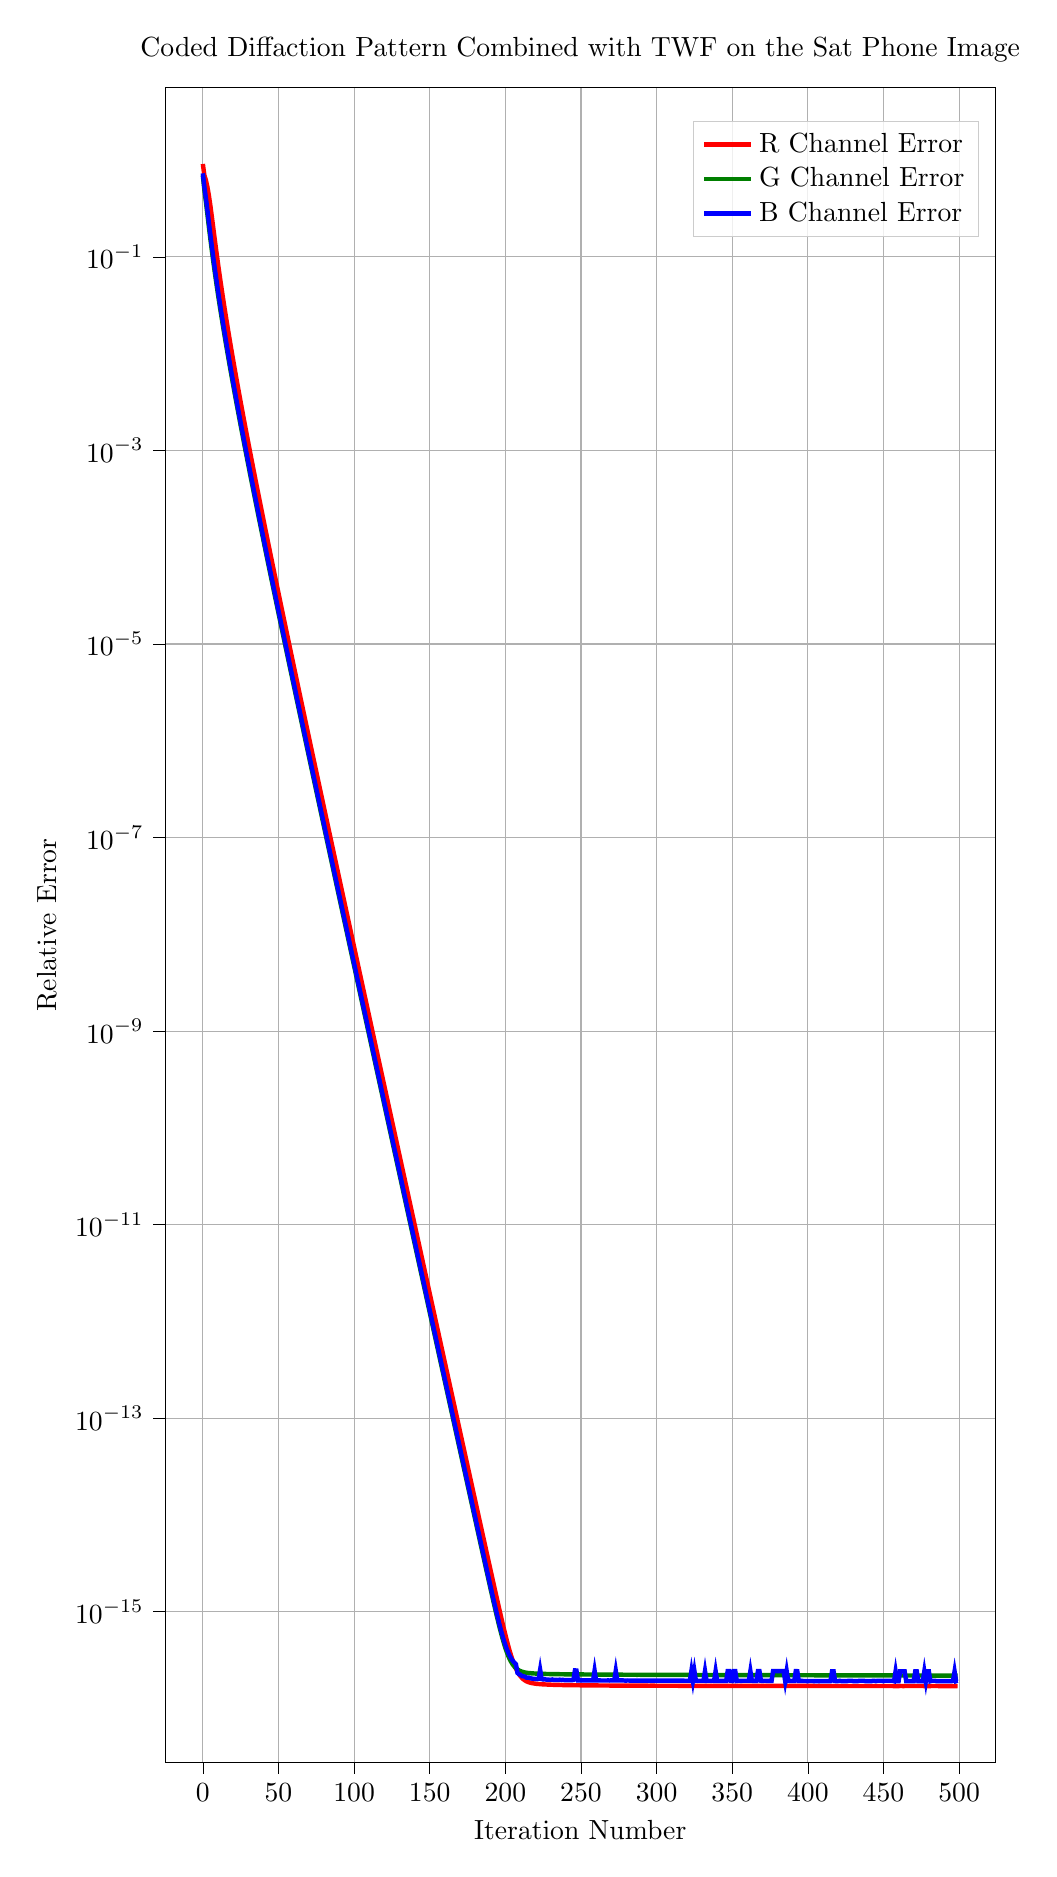
\begin{tikzpicture}

    \definecolor{darkgray176}{RGB}{176,176,176}
    \definecolor{green01270}{RGB}{0,127,0}
    \definecolor{lightgray204}{RGB}{204,204,204}
    
    \begin{axis}[
    width = 1.0\textwidth,
    height = 65em,
    legend cell align={left},
    legend style={fill opacity=0.8, draw opacity=1, text opacity=1, draw=lightgray204},
    log basis y={10},
    tick align=outside,
    tick pos=left,
    title={Coded Diffaction Pattern Combined with 
    \ac{TWF} on the Sat Phone Image},
    x grid style={darkgray176},
    xlabel={Iteration Number},
    xmajorgrids,
    xmin=-24.95, xmax=523.95,
    xtick style={color=black},
    y grid style={darkgray176},
    ylabel={Relative Error},
    ymajorgrids,
    ymin=2.78628737110491e-17, ymax=5.58364662598361,
    ymode=log,
    ytick style={color=black},
    ytick={1e-19,1e-17,1e-15,1e-13,1e-11,1e-09,1e-07,1e-05,0.001,0.1,10,1000},
    yticklabels={
      \(\displaystyle {10^{-19}}\),
      \(\displaystyle {10^{-17}}\),
      \(\displaystyle {10^{-15}}\),
      \(\displaystyle {10^{-13}}\),
      \(\displaystyle {10^{-11}}\),
      \(\displaystyle {10^{-9}}\),
      \(\displaystyle {10^{-7}}\),
      \(\displaystyle {10^{-5}}\),
      \(\displaystyle {10^{-3}}\),
      \(\displaystyle {10^{-1}}\),
      \(\displaystyle {10^{1}}\),
      \(\displaystyle {10^{3}}\)
    }
    ]
    \addplot [ultra thick, red]
    table {%
    0 0.912994766241893
    1 0.697827116743833
    2 0.622131526739553
    3 0.52817896682885
    4 0.430274379754422
    5 0.335854155374172
    6 0.255794614096927
    7 0.193298698901939
    8 0.14629791296794
    9 0.111407629801237
    10 0.0855233835495398
    11 0.0661988545979658
    12 0.0516428214317063
    13 0.0405721353756208
    14 0.0320780792169232
    15 0.025504675782994
    16 0.0203791990974184
    17 0.0163564929379512
    18 0.0131801482891011
    19 0.010658763379925
    20 0.00864764844050486
    21 0.00703651458605891
    22 0.0057407696101125
    23 0.00469488961293919
    24 0.00384810581151414
    25 0.00316050878544749
    26 0.00260062750044248
    27 0.00214366498597236
    28 0.00176985302617276
    29 0.00146341591961451
    30 0.00121171096296412
    31 0.00100460809915144
    32 0.000833909618231541
    33 0.000692998127413531
    34 0.000576512399016183
    35 0.000480074709373343
    36 0.000400140010574284
    37 0.000333806050517431
    38 0.00027869647504722
    39 0.000232865730291308
    40 0.000194712851548574
    41 0.000162922001531008
    42 0.000136410213743423
    43 0.000114282077188233
    44 9.57980972195361e-05
    45 8.03463188910596e-05
    46 6.74216047225008e-05
    47 5.66030486347542e-05
    48 4.75421073146164e-05
    49 3.99489324707876e-05
    50 3.35823288043861e-05
    51 2.82411641126094e-05
    52 2.3758170252001e-05
    53 1.99937524825916e-05
    54 1.6831411073166e-05
    55 1.41736388299464e-05
    56 1.19391052693918e-05
    57 1.00597409781772e-05
    58 8.47852557359361e-06
    59 7.14769570146904e-06
    60 6.02720741478282e-06
    61 5.08354624154834e-06
    62 4.28856613224358e-06
    63 3.61867571971731e-06
    64 3.05402713528674e-06
    65 2.5779738565515e-06
    66 2.17653671262694e-06
    67 1.83793391890368e-06
    68 1.55227042534524e-06
    69 1.31122237009316e-06
    70 1.10777238068588e-06
    71 9.36029508751954e-07
    72 7.91022781468164e-07
    73 6.68570881578766e-07
    74 5.65147771805746e-07
    75 4.77780025539953e-07
    76 4.03968156247396e-07
    77 3.4159789067041e-07
    78 2.88889961951471e-07
    79 2.44341426380264e-07
    80 2.06683594979919e-07
    81 1.74846341676509e-07
    82 1.47927185674174e-07
    83 1.25163775483454e-07
    84 1.05913009842119e-07
    85 8.9630723113965e-08
    86 7.58579338472612e-08
    87 6.42067787041143e-08
    88 5.43496124055449e-08
    89 4.60091319988436e-08
    90 3.89514180066543e-08
    91 3.29786397129868e-08
    92 2.79235994936191e-08
    93 2.36449667066643e-08
    94 2.00232281075211e-08
    95 1.69573152464985e-08
    96 1.43616916478371e-08
    97 1.21641095813128e-08
    98 1.0303369612088e-08
    99 8.72777050414225e-09
    100 7.39351462077961e-09
    101 6.26355691865475e-09
    102 5.306562164253e-09
    103 4.49602532185849e-09
    104 3.80948688601499e-09
    105 3.22792723461319e-09
    106 2.73528245678904e-09
    107 2.3179263107833e-09
    108 1.96433801358014e-09
    109 1.66475871659168e-09
    110 1.41092650188299e-09
    111 1.19584546305143e-09
    112 1.0135893840607e-09
    113 8.59148256887383e-10
    114 7.28269485085859e-10
    115 6.17352213557182e-10
    116 5.23345712104122e-10
    117 4.43669419965686e-10
    118 3.76136151671572e-10
    119 3.18894240985727e-10
    120 2.70373485325334e-10
    121 2.29242948267663e-10
    122 1.94376070817915e-10
    123 1.64817609574523e-10
    124 1.39758345183638e-10
    125 1.18512974818859e-10
    126 1.00500392416682e-10
    127 8.52282843705506e-11
    128 7.22791421214813e-11
    129 6.12992146826787e-11
    130 5.19888901737739e-11
    131 4.40940108917759e-11
    132 3.73991317606937e-11
    133 3.17216830253177e-11
    134 2.69068470801022e-11
    135 2.28234761820737e-11
    136 1.93603311827554e-11
    137 1.64230982295653e-11
    138 1.39318750280423e-11
    139 1.18188643944485e-11
    140 1.00265870998816e-11
    141 8.5063062808039e-12
    142 7.21671061357702e-12
    143 6.1227746699929e-12
    144 5.19479500568683e-12
    145 4.40757447259248e-12
    146 3.73973848908108e-12
    147 3.17317008605381e-12
    148 2.69249341167334e-12
    149 2.28468323453251e-12
    150 1.93868590210541e-12
    151 1.64512601598768e-12
    152 1.39604902044939e-12
    153 1.1847128992769e-12
    154 1.00539015485796e-12
    155 8.53229208427951e-13
    156 7.24113383874114e-13
    157 6.14551031882526e-13
    158 5.21578007737097e-13
    159 4.42679479034594e-13
    160 3.75723716348911e-13
    161 3.18902598615378e-13
    162 2.70680295101616e-13
    163 2.29754573296462e-13
    164 1.95021274248433e-13
    165 1.65542314543066e-13
    166 1.40522553383504e-13
    167 1.19286494108757e-13
    168 1.01262037741349e-13
    169 8.59624486207421e-14
    170 7.29761004681883e-14
    171 6.19530288735653e-14
    172 5.25960003744474e-14
    173 4.46531437941709e-14
    174 3.79104749294294e-14
    175 3.21869616087953e-14
    176 2.73282546391283e-14
    177 2.32034168794436e-14
    178 1.97018630770928e-14
    179 1.67290152470603e-14
    180 1.42054296441325e-14
    181 1.20629134602966e-14
    182 1.0244097875845e-14
    183 8.69995571719595e-15
    184 7.38915468589238e-15
    185 6.27616342000534e-15
    186 5.33131712353243e-15
    187 4.52943480149835e-15
    188 3.84877215420355e-15
    189 3.27075041344889e-15
    190 2.780428964171e-15
    191 2.36431721459162e-15
    192 2.01136204235618e-15
    193 1.71181593140141e-15
    194 1.45790305531565e-15
    195 1.24310628230564e-15
    196 1.06112526437377e-15
    197 9.07654947134406e-16
    198 7.77878451024904e-16
    199 6.68935918066592e-16
    200 5.77527046951957e-16
    201 5.01322674852452e-16
    202 4.37940344903624e-16
    203 3.85610923227176e-16
    204 3.4306166974065e-16
    205 3.08217076068382e-16
    206 2.80216132410129e-16
    207 2.57906983147772e-16
    208 2.40048147662173e-16
    209 2.26103289831196e-16
    210 2.15151538702045e-16
    211 2.06637846402666e-16
    212 1.99922816449147e-16
    213 1.94739003875257e-16
    214 1.90702252001177e-16
    215 1.87751403814742e-16
    216 1.85453627825972e-16
    217 1.83782276566795e-16
    218 1.82362466479503e-16
    219 1.81233861879096e-16
    220 1.8031514670002e-16
    221 1.79540912244077e-16
    222 1.78964679296435e-16
    223 1.78407346754576e-16
    224 1.77887951400112e-16
    225 1.77548026449768e-16
    226 1.77172779765071e-16
    227 1.76864428110068e-16
    228 1.76629901905104e-16
    229 1.76381385071411e-16
    230 1.7605740017857e-16
    231 1.75808767910822e-16
    232 1.75628339550254e-16
    233 1.75351581611586e-16
    234 1.75270857657168e-16
    235 1.75091905147875e-16
    236 1.74985505895688e-16
    237 1.74778884921928e-16
    238 1.74622253616199e-16
    239 1.74429862781474e-16
    240 1.74346662435949e-16
    241 1.74242533845552e-16
    242 1.74216370130129e-16
    243 1.74090868184106e-16
    244 1.73938305939907e-16
    245 1.7389572650322e-16
    246 1.73785993273311e-16
    247 1.73703791128993e-16
    248 1.73667805995322e-16
    249 1.73640647638574e-16
    250 1.73567825836047e-16
    251 1.73422109050415e-16
    252 1.73388641717991e-16
    253 1.73271138976082e-16
    254 1.73220975345738e-16
    255 1.73066813737199e-16
    256 1.73091832305094e-16
    257 1.73070782842733e-16
    258 1.72950691010456e-16
    259 1.72978252945556e-16
    260 1.72961653116174e-16
    261 1.72956235804602e-16
    262 1.72829877551892e-16
    263 1.72781906089817e-16
    264 1.72863415604391e-16
    265 1.72775293135383e-16
    266 1.72634585519217e-16
    267 1.72649569738741e-16
    268 1.72608893940474e-16
    269 1.72589091506446e-16
    270 1.72599436157028e-16
    271 1.72541557417486e-16
    272 1.72469916239255e-16
    273 1.72436519383838e-16
    274 1.7238561282566e-16
    275 1.72331487808895e-16
    276 1.72254570326254e-16
    277 1.72208087390113e-16
    278 1.72216478417152e-16
    279 1.72217422366001e-16
    280 1.72226933167287e-16
    281 1.72252869086607e-16
    282 1.72121263426392e-16
    283 1.72060677781086e-16
    284 1.72023038005243e-16
    285 1.72024183180453e-16
    286 1.71996770091912e-16
    287 1.71915278932674e-16
    288 1.71947205753923e-16
    289 1.71936876611878e-16
    290 1.71934785598855e-16
    291 1.71978103322626e-16
    292 1.71978193362398e-16
    293 1.719409002418e-16
    294 1.71894349153613e-16
    295 1.71847942398946e-16
    296 1.71895447547099e-16
    297 1.71919370163931e-16
    298 1.71899576756241e-16
    299 1.7187151074734e-16
    300 1.71795452735628e-16
    301 1.71750702312975e-16
    302 1.71723531743278e-16
    303 1.71746497739212e-16
    304 1.71796348589741e-16
    305 1.7175827609075e-16
    306 1.71709460811244e-16
    307 1.71695888243929e-16
    308 1.7170527986226e-16
    309 1.71666389753822e-16
    310 1.71688259500228e-16
    311 1.71646081841467e-16
    312 1.71635838367641e-16
    313 1.71609133699921e-16
    314 1.71576360665927e-16
    315 1.71488939997748e-16
    316 1.71449551521588e-16
    317 1.71522674387959e-16
    318 1.7152204539746e-16
    319 1.7146370753452e-16
    320 1.71366694083163e-16
    321 1.71367783442591e-16
    322 1.71315614891505e-16
    323 1.71292553801952e-16
    324 1.71325806985604e-16
    325 1.71367193312051e-16
    326 1.71312416848514e-16
    327 1.71321398094339e-16
    328 1.71365268268874e-16
    329 1.71403964070543e-16
    330 1.71396958006811e-16
    331 1.71386654597127e-16
    332 1.71356125300005e-16
    333 1.71299786143541e-16
    334 1.7138576138476e-16
    335 1.71375831595581e-16
    336 1.71345123160818e-16
    337 1.71380479712695e-16
    338 1.71221921456967e-16
    339 1.71240564245164e-16
    340 1.71195909428676e-16
    341 1.71260071061356e-16
    342 1.71235339049035e-16
    343 1.71196899965194e-16
    344 1.71203164312694e-16
    345 1.71196979053879e-16
    346 1.71170858821655e-16
    347 1.7118805470128e-16
    348 1.71155826695312e-16
    349 1.71190709922328e-16
    350 1.71175437349769e-16
    351 1.71227805091046e-16
    352 1.7119315796801e-16
    353 1.71117798576936e-16
    354 1.71101204643337e-16
    355 1.7106070741101e-16
    356 1.71024006608209e-16
    357 1.70992856372952e-16
    358 1.71080904430368e-16
    359 1.71067298504013e-16
    360 1.71114765936188e-16
    361 1.71115318441244e-16
    362 1.71053704413548e-16
    363 1.71105984551483e-16
    364 1.71140068867616e-16
    365 1.71070636087396e-16
    366 1.71035356725438e-16
    367 1.71108788753093e-16
    368 1.71088491644299e-16
    369 1.7105532310198e-16
    370 1.71062662149647e-16
    371 1.70984006552285e-16
    372 1.70990923887787e-16
    373 1.70954200123507e-16
    374 1.7098035104148e-16
    375 1.70913621414013e-16
    376 1.70883330332245e-16
    377 1.70884943283745e-16
    378 1.70944193763985e-16
    379 1.70934583752685e-16
    380 1.70942904273071e-16
    381 1.70929699158967e-16
    382 1.7098007509759e-16
    383 1.70946302509909e-16
    384 1.70955640277525e-16
    385 1.71024470836358e-16
    386 1.70963342569278e-16
    387 1.70826271784006e-16
    388 1.70859122357354e-16
    389 1.70866808333656e-16
    390 1.70938053282289e-16
    391 1.71031592470794e-16
    392 1.70957305688083e-16
    393 1.70866529648936e-16
    394 1.70907410013447e-16
    395 1.70904290937195e-16
    396 1.70916480873543e-16
    397 1.70891625898785e-16
    398 1.7087636544025e-16
    399 1.70878219499328e-16
    400 1.70915880757615e-16
    401 1.70895366686267e-16
    402 1.70968140542924e-16
    403 1.70954333439259e-16
    404 1.70880652097185e-16
    405 1.7083011425952e-16
    406 1.70813688014292e-16
    407 1.70849393487067e-16
    408 1.70838314324121e-16
    409 1.7077731281973e-16
    410 1.70833637139492e-16
    411 1.7080626941794e-16
    412 1.70769482082132e-16
    413 1.70769978879255e-16
    414 1.70786654663263e-16
    415 1.70727861444279e-16
    416 1.70755108400643e-16
    417 1.70796021053289e-16
    418 1.70738741092915e-16
    419 1.70739573509364e-16
    420 1.70756749860724e-16
    421 1.70673052561697e-16
    422 1.70697128584452e-16
    423 1.70673685863e-16
    424 1.70671338382592e-16
    425 1.70614935813844e-16
    426 1.70695241294184e-16
    427 1.70719736373238e-16
    428 1.7074128613127e-16
    429 1.70702598691589e-16
    430 1.70688641529045e-16
    431 1.70729185599657e-16
    432 1.70666440632652e-16
    433 1.70651202761236e-16
    434 1.70647013242039e-16
    435 1.70654451478602e-16
    436 1.70659125169944e-16
    437 1.70696136991762e-16
    438 1.70728077902974e-16
    439 1.70639080316577e-16
    440 1.70664373079924e-16
    441 1.70719592307517e-16
    442 1.70637618198185e-16
    443 1.70673033072839e-16
    444 1.70565513476993e-16
    445 1.70650861125545e-16
    446 1.70616176233593e-16
    447 1.7062748832811e-16
    448 1.70609261371096e-16
    449 1.70570830453755e-16
    450 1.70571730798605e-16
    451 1.70551203125549e-16
    452 1.70563929273801e-16
    453 1.70572873465263e-16
    454 1.705917619698e-16
    455 1.70594457802697e-16
    456 1.70568705049374e-16
    457 1.70481711930713e-16
    458 1.70500219711191e-16
    459 1.70540185452868e-16
    460 1.7054258886732e-16
    461 1.70565250755692e-16
    462 1.7059674370742e-16
    463 1.70508022715725e-16
    464 1.70565507562157e-16
    465 1.70570657806249e-16
    466 1.70605508302983e-16
    467 1.70559760615712e-16
    468 1.70583245764883e-16
    469 1.70615670654807e-16
    470 1.70636567526683e-16
    471 1.70587829200126e-16
    472 1.70616563750819e-16
    473 1.70598258693692e-16
    474 1.70588758399577e-16
    475 1.70605028684752e-16
    476 1.70554683130839e-16
    477 1.70533583992042e-16
    478 1.70527770302317e-16
    479 1.70493154822248e-16
    480 1.70510050685703e-16
    481 1.70533113255119e-16
    482 1.70600700456722e-16
    483 1.70581356528806e-16
    484 1.70655411012339e-16
    485 1.70613257868628e-16
    486 1.70552276808353e-16
    487 1.70480327921599e-16
    488 1.70506793469611e-16
    489 1.7047231448289e-16
    490 1.70503163108521e-16
    491 1.70427640213426e-16
    492 1.7044826944624e-16
    493 1.70402335850508e-16
    494 1.704622710423e-16
    495 1.70462652178909e-16
    496 1.70490680161496e-16
    497 1.70515570888912e-16
    498 1.70494525737071e-16
    499 1.70566333064942e-16
    };
    \addlegendentry{R Channel Error}
    \addplot [ultra thick, green01270]
    table {%
    0 0.693834731972221
    1 0.493310500544042
    2 0.373019686450051
    3 0.276186193273028
    4 0.204132692190209
    5 0.152131325553789
    6 0.114669297674848
    7 0.0874517432182047
    8 0.0674145271060658
    9 0.052464187132832
    10 0.0411654868337323
    11 0.032529165139785
    12 0.0258637455038854
    13 0.0206749591913691
    14 0.0166055495046518
    15 0.0133924806295977
    16 0.0108413571781619
    17 0.00880547971762989
    18 0.00717322644612723
    19 0.0058592276533411
    20 0.0047976458434604
    21 0.0039370455816062
    22 0.00323744788883349
    23 0.00266715115053193
    24 0.00220107984416324
    25 0.00181931135976231
    26 0.00150597132899782
    27 0.00124829471642943
    28 0.00103602211234911
    29 0.000860849273403757
    30 0.000716078640634018
    31 0.000596259311525643
    32 0.000496966085671391
    33 0.000414577460120864
    34 0.000346139702840445
    35 0.000289225938348932
    36 0.000241847420095666
    37 0.000202370847972615
    38 0.00016944959236948
    39 0.000141970311201421
    40 0.000119015257191364
    41 9.98258744758402e-05
    42 8.37743276303121e-05
    43 7.03377585145303e-05
    44 5.90831573319722e-05
    45 4.96504942505326e-05
    46 4.17406616459645e-05
    47 3.51043118467572e-05
    48 2.95338528841271e-05
    49 2.48558901644265e-05
    50 2.09257313482036e-05
    51 1.76224877993073e-05
    52 1.48449856953551e-05
    53 1.25087387652692e-05
    54 1.05429634658875e-05
    55 8.88838605517987e-06
    56 7.49526692998685e-06
    57 6.3219305266185e-06
    58 5.33341648622371e-06
    59 4.50041166135634e-06
    60 3.79824798145463e-06
    61 3.20623735983833e-06
    62 2.70699368428564e-06
    63 2.28587431540701e-06
    64 1.93058296051576e-06
    65 1.63077848728316e-06
    66 1.37774046816969e-06
    67 1.1641256598524e-06
    68 9.83766786652031e-07
    69 8.31457772812402e-07
    70 7.02816425387178e-07
    71 5.94150451456626e-07
    72 5.02343597255872e-07
    73 4.24769947317388e-07
    74 3.59212942254383e-07
    75 3.03804905022093e-07
    76 2.56968366499453e-07
    77 2.17372581943548e-07
    78 1.83895097448805e-07
    79 1.55587056911785e-07
    80 1.31647854802492e-07
    81 1.11401224014757e-07
    82 9.42759330552464e-08
    83 7.97894456865104e-08
    84 6.75338926087357e-08
    85 5.7164993709012e-08
    86 4.83913317335099e-08
    87 4.09670077451558e-08
    88 3.46840284262958e-08
    89 2.93665291840012e-08
    90 2.48658491142367e-08
    91 2.10562271425283e-08
    92 1.78313289762754e-08
    93 1.51011869255726e-08
    94 1.27897802042494e-08
    95 1.0832779126471e-08
    96 9.17567529469862e-09
    97 7.77245601689516e-09
    98 6.58415590566407e-09
    99 5.57780115353344e-09
    100 4.72546937982525e-09
    101 4.00356623616222e-09
    102 3.39211115722851e-09
    103 2.87416504848835e-09
    104 2.43541764194542e-09
    105 2.0637384022648e-09
    106 1.748856314368e-09
    107 1.48208201369312e-09
    108 1.25605498596554e-09
    109 1.06453874224307e-09
    110 9.02260352599219e-10
    111 7.6475072710204e-10
    112 6.48221538717866e-10
    113 5.49470723460648e-10
    114 4.65779679760141e-10
    115 3.9485146418627e-10
    116 3.34736198870006e-10
    117 2.83782952965264e-10
    118 2.40593782324043e-10
    119 2.03984192717663e-10
    120 1.72950681647616e-10
    121 1.46642864533127e-10
    122 1.24341022448887e-10
    123 1.05434112212693e-10
    124 8.94047281836946e-11
    125 7.58146935261139e-11
    126 6.42923395248985e-11
    127 5.45228611042384e-11
    128 4.62391795207839e-11
    129 3.92152701855994e-11
    130 3.32592365649202e-11
    131 2.82085856985645e-11
    132 2.39255612287915e-11
    133 2.02934298150367e-11
    134 1.72132058966308e-11
    135 1.4600900554962e-11
    136 1.23853705639218e-11
    137 1.05063048940778e-11
    138 8.91254102998549e-12
    139 7.56074045285912e-12
    140 6.414133729942e-12
    141 5.44154905223115e-12
    142 4.61654208475658e-12
    143 3.9167116547799e-12
    144 3.32304774982556e-12
    145 2.8194352240661e-12
    146 2.39220316539213e-12
    147 2.02975663005581e-12
    148 1.72226501876887e-12
    149 1.46139204257822e-12
    150 1.24006185259177e-12
    151 1.05227466618878e-12
    152 8.92943426760908e-13
    153 7.57754085787622e-13
    154 6.43046511203799e-13
    155 5.45713977196536e-13
    156 4.63123332721044e-13
    157 3.93041608461907e-13
    158 3.33571145922149e-13
    159 2.8310567020205e-13
    160 2.40279974761741e-13
    161 2.03936513732574e-13
    162 1.73094082511911e-13
    163 1.46918930057355e-13
    164 1.24704595413504e-13
    165 1.05850979663288e-13
    166 8.98495039823355e-14
    167 7.62690492441015e-14
    168 6.47413214268236e-14
    169 5.49578130983738e-14
    170 4.66536937089976e-14
    171 3.96052219450826e-14
    172 3.36223232261869e-14
    173 2.85442706496993e-14
    174 2.42336655763261e-14
    175 2.05745578566999e-14
    176 1.74682161204837e-14
    177 1.48316018406497e-14
    178 1.25932868104241e-14
    179 1.06932699006525e-14
    180 9.08046641787743e-15
    181 7.71131853853063e-15
    182 6.5493562128215e-15
    183 5.56287481647248e-15
    184 4.72577236819615e-15
    185 4.0154040810454e-15
    186 3.41267095279191e-15
    187 2.90121310546815e-15
    188 2.4677087354934e-15
    189 2.09989335954628e-15
    190 1.78851325221705e-15
    191 1.52452983539191e-15
    192 1.30106651615598e-15
    193 1.11266288454128e-15
    194 9.53702726344638e-16
    195 8.20161992684981e-16
    196 7.08381781284837e-16
    197 6.15233821452326e-16
    198 5.38236158899511e-16
    199 4.74631498158094e-16
    200 4.22802798948812e-16
    201 3.80861357766892e-16
    202 3.47271825065096e-16
    203 3.20589125405467e-16
    204 2.99718955215039e-16
    205 2.83446084628853e-16
    206 2.70854866089761e-16
    207 2.61087170708644e-16
    208 2.53531403689188e-16
    209 2.4772833504688e-16
    210 2.43241704826161e-16
    211 2.39960363367675e-16
    212 2.37397216933216e-16
    213 2.3539884011881e-16
    214 2.33920988816262e-16
    215 2.3280322965195e-16
    216 2.31828959767897e-16
    217 2.31037902067775e-16
    218 2.30401764766162e-16
    219 2.29920910442266e-16
    220 2.29463950914698e-16
    221 2.2904297727846e-16
    222 2.28680357506617e-16
    223 2.28354441378296e-16
    224 2.28033733151198e-16
    225 2.27752389593257e-16
    226 2.27536945456157e-16
    227 2.27284603531643e-16
    228 2.27082191262217e-16
    229 2.26929895237725e-16
    230 2.26754215577616e-16
    231 2.26655523897311e-16
    232 2.26545172244628e-16
    233 2.26388868651954e-16
    234 2.26320410943229e-16
    235 2.26074915135572e-16
    236 2.2592127892842e-16
    237 2.25784237395222e-16
    238 2.2563647067194e-16
    239 2.25517382989632e-16
    240 2.25414414273311e-16
    241 2.25332358026431e-16
    242 2.25229963853162e-16
    243 2.25120818548569e-16
    244 2.25093528350261e-16
    245 2.25047699257527e-16
    246 2.25000352373289e-16
    247 2.24934865226858e-16
    248 2.24906027827432e-16
    249 2.2481768707146e-16
    250 2.24728502540838e-16
    251 2.24678789286e-16
    252 2.24602163572533e-16
    253 2.24528700299335e-16
    254 2.24423095496671e-16
    255 2.24396527071107e-16
    256 2.24378893361007e-16
    257 2.24253817462391e-16
    258 2.24239189805478e-16
    259 2.24210081396346e-16
    260 2.24137038696194e-16
    261 2.24133243439518e-16
    262 2.24050357240561e-16
    263 2.24001546577084e-16
    264 2.23956622902862e-16
    265 2.23924775402746e-16
    266 2.23879616101993e-16
    267 2.23790537628637e-16
    268 2.23712531727515e-16
    269 2.23672080078939e-16
    270 2.23645520546701e-16
    271 2.23652757834352e-16
    272 2.23543045665388e-16
    273 2.23489425895495e-16
    274 2.23475505853321e-16
    275 2.23370776936296e-16
    276 2.23349931825308e-16
    277 2.23334477932303e-16
    278 2.23252455176781e-16
    279 2.23227239757133e-16
    280 2.23170082459945e-16
    281 2.23135790596656e-16
    282 2.23136607798172e-16
    283 2.23064725467166e-16
    284 2.23009776877896e-16
    285 2.22971562422413e-16
    286 2.22933532508558e-16
    287 2.22852734799159e-16
    288 2.22908692490847e-16
    289 2.22883015187382e-16
    290 2.22800568538798e-16
    291 2.22784063012351e-16
    292 2.22768702887248e-16
    293 2.22741155561337e-16
    294 2.22715882969292e-16
    295 2.22691349487521e-16
    296 2.22680320610343e-16
    297 2.2260717861097e-16
    298 2.2259144785609e-16
    299 2.22560587611608e-16
    300 2.22514088486338e-16
    301 2.22436744377783e-16
    302 2.22425456936487e-16
    303 2.22381940131959e-16
    304 2.22383768414409e-16
    305 2.22407891492447e-16
    306 2.22442958565933e-16
    307 2.22367788835158e-16
    308 2.22352111752315e-16
    309 2.22329729490546e-16
    310 2.222929907572e-16
    311 2.22248035277747e-16
    312 2.22239353741677e-16
    313 2.22200217314495e-16
    314 2.22227199669878e-16
    315 2.22192739079773e-16
    316 2.22122695541426e-16
    317 2.22092024959531e-16
    318 2.220699002382e-16
    319 2.22084817147934e-16
    320 2.22064944507798e-16
    321 2.21993166128847e-16
    322 2.21945062202225e-16
    323 2.21973208582561e-16
    324 2.21924306711299e-16
    325 2.21867498667199e-16
    326 2.21862904452253e-16
    327 2.2186344703964e-16
    328 2.21866914998e-16
    329 2.21849056109202e-16
    330 2.21802348508153e-16
    331 2.21767039237428e-16
    332 2.21774827636586e-16
    333 2.21699968361649e-16
    334 2.21680227505802e-16
    335 2.21653575325986e-16
    336 2.21603210106062e-16
    337 2.21611071472095e-16
    338 2.21550083031369e-16
    339 2.21549201452641e-16
    340 2.21573693204617e-16
    341 2.21532234882243e-16
    342 2.21510211781472e-16
    343 2.2146474430181e-16
    344 2.21463648307016e-16
    345 2.21423993223294e-16
    346 2.21454275468002e-16
    347 2.21380743759898e-16
    348 2.2132375526225e-16
    349 2.21322998316804e-16
    350 2.21283471378237e-16
    351 2.21240335862778e-16
    352 2.21263627092168e-16
    353 2.2126048609376e-16
    354 2.21214936962081e-16
    355 2.21240883710565e-16
    356 2.21205895933823e-16
    357 2.21199145996716e-16
    358 2.21183379528828e-16
    359 2.21187179661513e-16
    360 2.21165664985687e-16
    361 2.21161032824773e-16
    362 2.2104602598357e-16
    363 2.21064668001148e-16
    364 2.21019584620371e-16
    365 2.21022797559085e-16
    366 2.20972338000076e-16
    367 2.20927847070721e-16
    368 2.20935708611487e-16
    369 2.20880457525964e-16
    370 2.20901697526575e-16
    371 2.20928960371706e-16
    372 2.20896986214805e-16
    373 2.20856110952777e-16
    374 2.20827349083506e-16
    375 2.20755226282038e-16
    376 2.20702331014827e-16
    377 2.20697610030965e-16
    378 2.20632072724797e-16
    379 2.20614328560802e-16
    380 2.20582145403067e-16
    381 2.20590276503709e-16
    382 2.20568998584629e-16
    383 2.20534997971222e-16
    384 2.20526473611001e-16
    385 2.20511393189412e-16
    386 2.20456929341538e-16
    387 2.20492637366105e-16
    388 2.2044420544596e-16
    389 2.20392435760776e-16
    390 2.20368755854984e-16
    391 2.20436943451084e-16
    392 2.2036751215123e-16
    393 2.20409438490381e-16
    394 2.20353593500131e-16
    395 2.20318797679733e-16
    396 2.20301500331073e-16
    397 2.20301722102096e-16
    398 2.20315642252272e-16
    399 2.2032319944518e-16
    400 2.20312836271187e-16
    401 2.20318927133527e-16
    402 2.20326480376043e-16
    403 2.20299962055049e-16
    404 2.20262948943181e-16
    405 2.20215721340435e-16
    406 2.20246382870498e-16
    407 2.20225093212368e-16
    408 2.20214902544556e-16
    409 2.20138374533226e-16
    410 2.20134091137426e-16
    411 2.20113011932401e-16
    412 2.20150368449115e-16
    413 2.20150419278221e-16
    414 2.20122593724081e-16
    415 2.20088010825586e-16
    416 2.20086174476192e-16
    417 2.20042037821145e-16
    418 2.20026810300295e-16
    419 2.20012751676013e-16
    420 2.1998166577346e-16
    421 2.19995684036124e-16
    422 2.19975007507361e-16
    423 2.19969312210258e-16
    424 2.19939783796492e-16
    425 2.19922204247397e-16
    426 2.1991876884807e-16
    427 2.19895221883294e-16
    428 2.1983703389555e-16
    429 2.19898123211407e-16
    430 2.19859527329476e-16
    431 2.19822175527016e-16
    432 2.19827375486584e-16
    433 2.1981553168905e-16
    434 2.1977786851906e-16
    435 2.19738570384384e-16
    436 2.19661837918098e-16
    437 2.19711303254514e-16
    438 2.19644350513944e-16
    439 2.19616519103842e-16
    440 2.19660604224516e-16
    441 2.19599885691592e-16
    442 2.19593289859161e-16
    443 2.19609113172981e-16
    444 2.19572215523969e-16
    445 2.19510886851371e-16
    446 2.19499136605494e-16
    447 2.19542437657714e-16
    448 2.19478241623293e-16
    449 2.19532869872522e-16
    450 2.19510682507817e-16
    451 2.19431689519638e-16
    452 2.19412666150989e-16
    453 2.19366235548009e-16
    454 2.19355863494724e-16
    455 2.19375130295721e-16
    456 2.19346284808687e-16
    457 2.19273301465813e-16
    458 2.19247976332969e-16
    459 2.19269005327813e-16
    460 2.19240762447102e-16
    461 2.19210640638033e-16
    462 2.19151394395424e-16
    463 2.19158961289436e-16
    464 2.19156648858517e-16
    465 2.19207473765012e-16
    466 2.19161773900849e-16
    467 2.19146500322603e-16
    468 2.19171375147551e-16
    469 2.19136345061325e-16
    470 2.19043942402479e-16
    471 2.19076847378636e-16
    472 2.19007615689225e-16
    473 2.19080301438515e-16
    474 2.19060785864316e-16
    475 2.19008810349346e-16
    476 2.19002034557153e-16
    477 2.18996326425845e-16
    478 2.19011708228589e-16
    479 2.19018352656933e-16
    480 2.18960129693663e-16
    481 2.18981337019743e-16
    482 2.18906119079358e-16
    483 2.18927883662481e-16
    484 2.18906161620487e-16
    485 2.18884578306134e-16
    486 2.18806542505549e-16
    487 2.18844870100232e-16
    488 2.18880953012751e-16
    489 2.18789678812838e-16
    490 2.18757996325748e-16
    491 2.18714040186007e-16
    492 2.18670111120992e-16
    493 2.18743431251703e-16
    494 2.18651024125481e-16
    495 2.18620064153898e-16
    496 2.18602347314281e-16
    497 2.18604470793947e-16
    498 2.18592618340607e-16
    499 2.18579930700646e-16
    };
    \addlegendentry{G Channel Error}
    \addplot [ultra thick, blue]
    table {%
    0 0.730600316765924
    1 0.526517130213586
    2 0.406658836733099
    3 0.303990196540131
    4 0.225199843213572
    5 0.167647988860099
    6 0.126038033529133
    7 0.0958167512166313
    8 0.0736305496518787
    9 0.0571299517841461
    10 0.0447039408781512
    11 0.035240486991524
    12 0.0279578813344458
    13 0.0223053193247083
    14 0.0178831241397214
    15 0.0144000243898699
    16 0.0116399887253952
    17 0.00944153881135583
    18 0.007682012622388
    19 0.00626778465048367
    20 0.00512688756853109
    21 0.00420330764077629
    22 0.00345337520283755
    23 0.00284274626121887
    24 0.0023442183331572
    25 0.00193628759110809
    26 0.00160176567595744
    27 0.00132688956970497
    28 0.00110061336887364
    29 0.000914032799411558
    30 0.000759932247682727
    31 0.000632472936767281
    32 0.000526908410408163
    33 0.000439364362466557
    34 0.00036668195150388
    35 0.000306271928008035
    36 0.000256007480510374
    37 0.000214144113307529
    38 0.000179246652145193
    39 0.000150130952260569
    40 0.000125819422298621
    41 0.00010550402575767
    42 8.85153407972425e-05
    43 7.42992418234251e-05
    44 6.23953290479566e-05
    45 5.24217833518252e-05
    46 4.40605736677956e-05
    47 3.70476258050038e-05
    48 3.11626661339893e-05
    49 2.62218742429583e-05
    50 2.20719148970595e-05
    51 1.85846613205797e-05
    52 1.56530931794991e-05
    53 1.31877342676977e-05
    54 1.11137022570081e-05
    55 9.3682576451026e-06
    56 7.89888521893867e-06
    57 6.66158044540977e-06
    58 5.61933523116705e-06
    59 4.74116358726916e-06
    60 4.00102488622263e-06
    61 3.37708268773903e-06
    62 2.85096288166847e-06
    63 2.40721958681202e-06
    64 2.03288453102447e-06
    65 1.71703959194769e-06
    66 1.45048993907626e-06
    67 1.22549755113953e-06
    68 1.03554919981342e-06
    69 8.75157452596904e-07
    70 7.39704741108819e-07
    71 6.25293934058877e-07
    72 5.28641496324103e-07
    73 4.46981947854308e-07
    74 3.77978220059361e-07
    75 3.19660247479072e-07
    76 2.7036742055893e-07
    77 2.28698505764342e-07
    78 1.93469491602764e-07
    79 1.63681819915187e-07
    80 1.38492393949285e-07
    81 1.17189528760874e-07
    82 9.91712823163472e-08
    83 8.39299712448531e-08
    84 7.10362390893811e-08
    85 6.01276312042332e-08
    86 5.08978168283385e-08
    87 4.30878301180486e-08
    88 3.64786610230585e-08
    89 3.08852773408752e-08
    90 2.61511931338435e-08
    91 2.21440795458059e-08
    92 1.87521304971365e-08
    93 1.58806983074675e-08
    94 1.34497127392931e-08
    95 1.13914882948691e-08
    96 9.6487696125449e-09
    97 8.17308367562341e-09
    98 6.92344665414059e-09
    99 5.86516743066308e-09
    100 4.96888623468552e-09
    101 4.20977281422878e-09
    102 3.5667907313895e-09
    103 3.02215260465666e-09
    104 2.56079243890515e-09
    105 2.1699588229653e-09
    106 1.83884873485106e-09
    107 1.55832846051956e-09
    108 1.32065297315917e-09
    109 1.11927484995603e-09
    110 9.48640281076715e-10
    111 8.0404830646766e-10
    112 6.81520765417189e-10
    113 5.77686568135726e-10
    114 4.89691569433605e-10
    115 4.15115182599193e-10
    116 3.51909676497535e-10
    117 2.98337810255481e-10
    118 2.52929935355597e-10
    119 2.14440299878538e-10
    120 1.81814264138652e-10
    121 1.54156956061639e-10
    122 1.30710975736462e-10
    123 1.10834347070438e-10
    124 9.39832495174063e-11
    125 7.96963409926241e-11
    126 6.75832669474523e-11
    127 5.73130610158309e-11
    128 4.86049785352684e-11
    129 4.12212224526144e-11
    130 3.49601769722014e-11
    131 2.96509717914349e-11
    132 2.5148708505352e-11
    133 2.13307071569318e-11
    134 1.80928636526512e-11
    135 1.53468774179634e-11
    136 1.30179630115097e-11
    137 1.10427537130109e-11
    138 9.36747555069332e-12
    139 7.94655028927382e-12
    140 6.74133123404674e-12
    141 5.71904232918155e-12
    142 4.85190392024647e-12
    143 4.11633626805006e-12
    144 3.49236946951652e-12
    145 2.9630522804462e-12
    146 2.51402180919199e-12
    147 2.13308566790463e-12
    148 1.80991250819573e-12
    149 1.53573677638594e-12
    150 1.30312440787699e-12
    151 1.1057678979158e-12
    152 9.38323621719582e-13
    153 7.96248334153796e-13
    154 6.75700803810626e-13
    155 5.73418857435197e-13
    156 4.86625639972034e-13
    157 4.12979786224857e-13
    158 3.50486316028691e-13
    159 2.97455642021966e-13
    160 2.52455720612451e-13
    161 2.14265607174297e-13
    162 1.81857395649561e-13
    163 1.54354090534009e-13
    164 1.31013019485785e-13
    165 1.11206315329703e-13
    166 9.43916548633007e-14
    167 8.0122805621491e-14
    168 6.80125457170532e-14
    169 5.77338986768632e-14
    170 4.9009617260077e-14
    171 4.16045548866632e-14
    172 3.53194448401853e-14
    173 2.99855207138955e-14
    174 2.54567154227603e-14
    175 2.16116886778572e-14
    176 1.83497144825638e-14
    177 1.55797665314883e-14
    178 1.32294836842721e-14
    179 1.12337819791298e-14
    180 9.53840062685466e-15
    181 8.10117734270261e-15
    182 6.88054646169988e-15
    183 5.84424892410554e-15
    184 4.96457815883345e-15
    185 4.21809520034026e-15
    186 3.58436340971104e-15
    187 3.04802896884408e-15
    188 2.59235856977461e-15
    189 2.20644963785118e-15
    190 1.87930986681223e-15
    191 1.60230520884829e-15
    192 1.36857097528871e-15
    193 1.17096179866442e-15
    194 1.00477203512377e-15
    195 8.65085239790709e-16
    196 7.48527522786132e-16
    197 6.51603915217073e-16
    198 5.71531141765478e-16
    199 5.05817566872538e-16
    200 4.52268272861859e-16
    201 4.09059075431575e-16
    202 3.74520738065932e-16
    203 3.47259058777487e-16
    204 3.2595084166526e-16
    205 3.09367959949729e-16
    206 2.96420241979852e-16
    207 2.86373106740906e-16
    208 2.33300463388233e-16
    209 2.26061737432896e-16
    210 2.23184567941293e-16
    211 2.16064453896242e-16
    212 2.15384627956007e-16
    213 2.12644408809207e-16
    214 2.08057836650111e-16
    215 2.08969457341211e-16
    216 2.07549461122371e-16
    217 2.04070076923578e-16
    218 2.03205594718562e-16
    219 2.02415243015084e-16
    220 2.01808800467045e-16
    221 2.0110674928688e-16
    222 2.0264561199016e-16
    223 2.51203820247291e-16
    224 2.01681304060979e-16
    225 1.99429611151876e-16
    226 2.00942398061262e-16
    227 1.9873020901412e-16
    228 1.98490291236032e-16
    229 1.9826823563425e-16
    230 1.98025540983388e-16
    231 1.99435683999526e-16
    232 1.97547569584785e-16
    233 1.97306364682345e-16
    234 1.97172257385442e-16
    235 1.96993850265782e-16
    236 1.9841164829767e-16
    237 1.9669520517933e-16
    238 1.98055561759565e-16
    239 1.96394601442958e-16
    240 1.9632181868334e-16
    241 1.96192579385723e-16
    242 1.96118872523648e-16
    243 1.96002154239609e-16
    244 1.95896075835944e-16
    245 1.97147525318063e-16
    246 2.47085210036087e-16
    247 2.4699419224892e-16
    248 1.9543266125345e-16
    249 1.95382074349306e-16
    250 1.95372502434783e-16
    251 1.95373547617319e-16
    252 1.95260979893387e-16
    253 1.953298735014e-16
    254 1.95268924447442e-16
    255 1.95155112767934e-16
    256 1.95132420312224e-16
    257 1.95060063018926e-16
    258 1.95015976165053e-16
    259 2.46098844985124e-16
    260 1.94836322048762e-16
    261 1.9481153721636e-16
    262 1.95563138244128e-16
    263 1.94666198667453e-16
    264 1.94497714296019e-16
    265 1.94540552756526e-16
    266 1.94513246407388e-16
    267 1.94470796279759e-16
    268 1.95202454292837e-16
    269 1.94462416009641e-16
    270 1.95211733125135e-16
    271 1.9518942177144e-16
    272 1.95116047854674e-16
    273 2.45510716816436e-16
    274 1.95044573147724e-16
    275 1.94919154863838e-16
    276 1.94911606805997e-16
    277 1.94885966523258e-16
    278 1.9479590515036e-16
    279 1.94313748744683e-16
    280 1.9428454885106e-16
    281 1.94738302438796e-16
    282 1.94237718596147e-16
    283 1.94341581978797e-16
    284 1.94268762788594e-16
    285 1.9424061846977e-16
    286 1.94172250617568e-16
    287 1.94132815213951e-16
    288 1.94058154224054e-16
    289 1.93955338280276e-16
    290 1.93938861182516e-16
    291 1.93848998439041e-16
    292 1.93830056099517e-16
    293 1.93911599658548e-16
    294 1.9387330260576e-16
    295 1.94087423584926e-16
    296 1.93845833079105e-16
    297 1.93852882153469e-16
    298 1.93773556452333e-16
    299 1.93800511532957e-16
    300 1.93844449332773e-16
    301 1.93852299916649e-16
    302 1.93849626714705e-16
    303 1.93817684540142e-16
    304 1.93826025931397e-16
    305 1.93857563281831e-16
    306 1.9385361280475e-16
    307 1.93849792907972e-16
    308 1.93928736267929e-16
    309 1.9373719708841e-16
    310 1.93742745043644e-16
    311 1.93701939366448e-16
    312 1.93764931351444e-16
    313 1.93761651152332e-16
    314 1.93788498523255e-16
    315 1.93764879540028e-16
    316 1.93761596054987e-16
    317 1.93732384038254e-16
    318 1.93619975633343e-16
    319 1.9353104278133e-16
    320 1.93458019832648e-16
    321 1.93503996407311e-16
    322 1.93592060044901e-16
    323 2.44025596783338e-16
    324 1.93358753866857e-16
    325 2.43814724137039e-16
    326 1.93295690983573e-16
    327 1.93242640125494e-16
    328 1.93564929231148e-16
    329 1.93582686754573e-16
    330 1.93572335614753e-16
    331 1.93645940780877e-16
    332 2.43721617993939e-16
    333 1.93184974235482e-16
    334 1.93584458009695e-16
    335 1.93554099529905e-16
    336 1.93059049103436e-16
    337 1.93559430648563e-16
    338 1.92953434643948e-16
    339 2.43573512739561e-16
    340 1.92927132622385e-16
    341 1.92939725788215e-16
    342 1.92947318651481e-16
    343 1.92941759899967e-16
    344 1.92902567920647e-16
    345 1.92922652691536e-16
    346 1.92879375800377e-16
    347 2.43360578109893e-16
    348 2.43374845552983e-16
    349 1.93570154387046e-16
    350 1.928211339264e-16
    351 2.43288269671185e-16
    352 2.43291435887515e-16
    353 1.92783944513237e-16
    354 1.93538417004384e-16
    355 1.9350402676877e-16
    356 1.92769838090172e-16
    357 1.9348056360864e-16
    358 1.93451983992791e-16
    359 1.93457782758014e-16
    360 1.93440883129623e-16
    361 1.93517010014221e-16
    362 2.43192774525229e-16
    363 1.93521648653798e-16
    364 1.92657619501148e-16
    365 1.92713648622539e-16
    366 1.92648370521588e-16
    367 2.43090248360519e-16
    368 2.43096693840857e-16
    369 1.93483719648121e-16
    370 1.92519948036781e-16
    371 1.93418533844299e-16
    372 1.93434287929169e-16
    373 1.92477312763097e-16
    374 1.92525214033993e-16
    375 1.92494556969756e-16
    376 1.92479751343122e-16
    377 2.4298062710409e-16
    378 2.42937123828058e-16
    379 2.42884981037486e-16
    380 2.42874734196397e-16
    381 2.42812834328502e-16
    382 2.42753848660336e-16
    383 2.42744116611711e-16
    384 2.42734491087491e-16
    385 1.92243418905172e-16
    386 2.4277316816682e-16
    387 1.92349189901765e-16
    388 1.93511685487297e-16
    389 1.92326224172862e-16
    390 1.92242180494955e-16
    391 1.92315223490212e-16
    392 2.42770447964987e-16
    393 2.42680401242117e-16
    394 1.9222145289499e-16
    395 1.92189684861641e-16
    396 1.93457221230499e-16
    397 1.9220825282424e-16
    398 1.92163589926656e-16
    399 1.92112487731257e-16
    400 1.92072355151776e-16
    401 1.92140386865157e-16
    402 1.92136717299817e-16
    403 1.92149410739936e-16
    404 1.92067190721761e-16
    405 1.92058732132533e-16
    406 1.92113261881095e-16
    407 1.92102158207779e-16
    408 1.92079061664067e-16
    409 1.92056082879137e-16
    410 1.91994808745869e-16
    411 1.92056125536892e-16
    412 1.92042712015499e-16
    413 1.9200760511793e-16
    414 1.92003333054513e-16
    415 1.92066907412076e-16
    416 2.42507324096161e-16
    417 2.42488588658889e-16
    418 1.92117316542344e-16
    419 1.92025446494857e-16
    420 1.92002705224384e-16
    421 1.93439102399817e-16
    422 1.91949819245565e-16
    423 1.91879804055426e-16
    424 1.91950076111352e-16
    425 1.91902603355955e-16
    426 1.91886087647148e-16
    427 1.93484173774595e-16
    428 1.93473486453479e-16
    429 1.93475716242446e-16
    430 1.91770473442717e-16
    431 1.91784303905896e-16
    432 1.91778548583349e-16
    433 1.91839463603775e-16
    434 1.93327046296485e-16
    435 1.93350088586671e-16
    436 1.93405778242251e-16
    437 1.93432576512048e-16
    438 1.91751853528283e-16
    439 1.91722396568216e-16
    440 1.91723512494591e-16
    441 1.91706665077067e-16
    442 1.91730334035182e-16
    443 1.93362879374538e-16
    444 1.93366208469069e-16
    445 1.91614672360531e-16
    446 1.9336265894741e-16
    447 1.93370340954734e-16
    448 1.93344603904869e-16
    449 1.93316464049026e-16
    450 1.91508568349045e-16
    451 1.93361313255714e-16
    452 1.93318464772881e-16
    453 1.93265368922816e-16
    454 1.93322773585971e-16
    455 1.93285477903543e-16
    456 1.93372596503028e-16
    457 1.91434340193803e-16
    458 2.41772805396028e-16
    459 1.91484310281962e-16
    460 1.91549705898418e-16
    461 2.4171937512261e-16
    462 2.41772168736756e-16
    463 2.41790865912958e-16
    464 2.41747328972191e-16
    465 1.91527064667154e-16
    466 1.91514900212643e-16
    467 1.91497641053891e-16
    468 1.91500865936577e-16
    469 1.91526621707557e-16
    470 1.91445322847798e-16
    471 2.41657584335332e-16
    472 2.41611113149421e-16
    473 1.91484676693095e-16
    474 1.91508275921341e-16
    475 1.91507064522903e-16
    476 1.91565583163985e-16
    477 2.41787118557201e-16
    478 1.91513789229238e-16
    479 2.41761076644158e-16
    480 2.41736006642737e-16
    481 1.91407273466622e-16
    482 1.9350556958866e-16
    483 1.93481603703776e-16
    484 1.9351178875805e-16
    485 1.91438112209653e-16
    486 1.914232355773e-16
    487 1.9138276352661e-16
    488 1.91330553825279e-16
    489 1.91340772509078e-16
    490 1.91339834979849e-16
    491 1.91408156224278e-16
    492 1.91370860141745e-16
    493 1.91351533136725e-16
    494 1.91319485316804e-16
    495 1.9130703911714e-16
    496 1.93503655359942e-16
    497 2.41490052265029e-16
    498 1.9129647314591e-16
    499 1.93610787292023e-16
    };
    \addlegendentry{B Channel Error}
    \end{axis}
    
    \end{tikzpicture}
    
    % \end{turn}
    \caption{TWF on the sat phone using coded diffraction pattern}
      \label{fig:twf_sat_phone_error}
    \end{figure}
  % \clearpage % End the page
}
\afterpage{%
  % \clearpage % Start a new page
    
    \begin{figure}[!htbp]
      \centering
    \captionsetup{justification=centering}
    % \begin{turn}{-90}
      % This file was created with tikzplotlib v0.10.1.
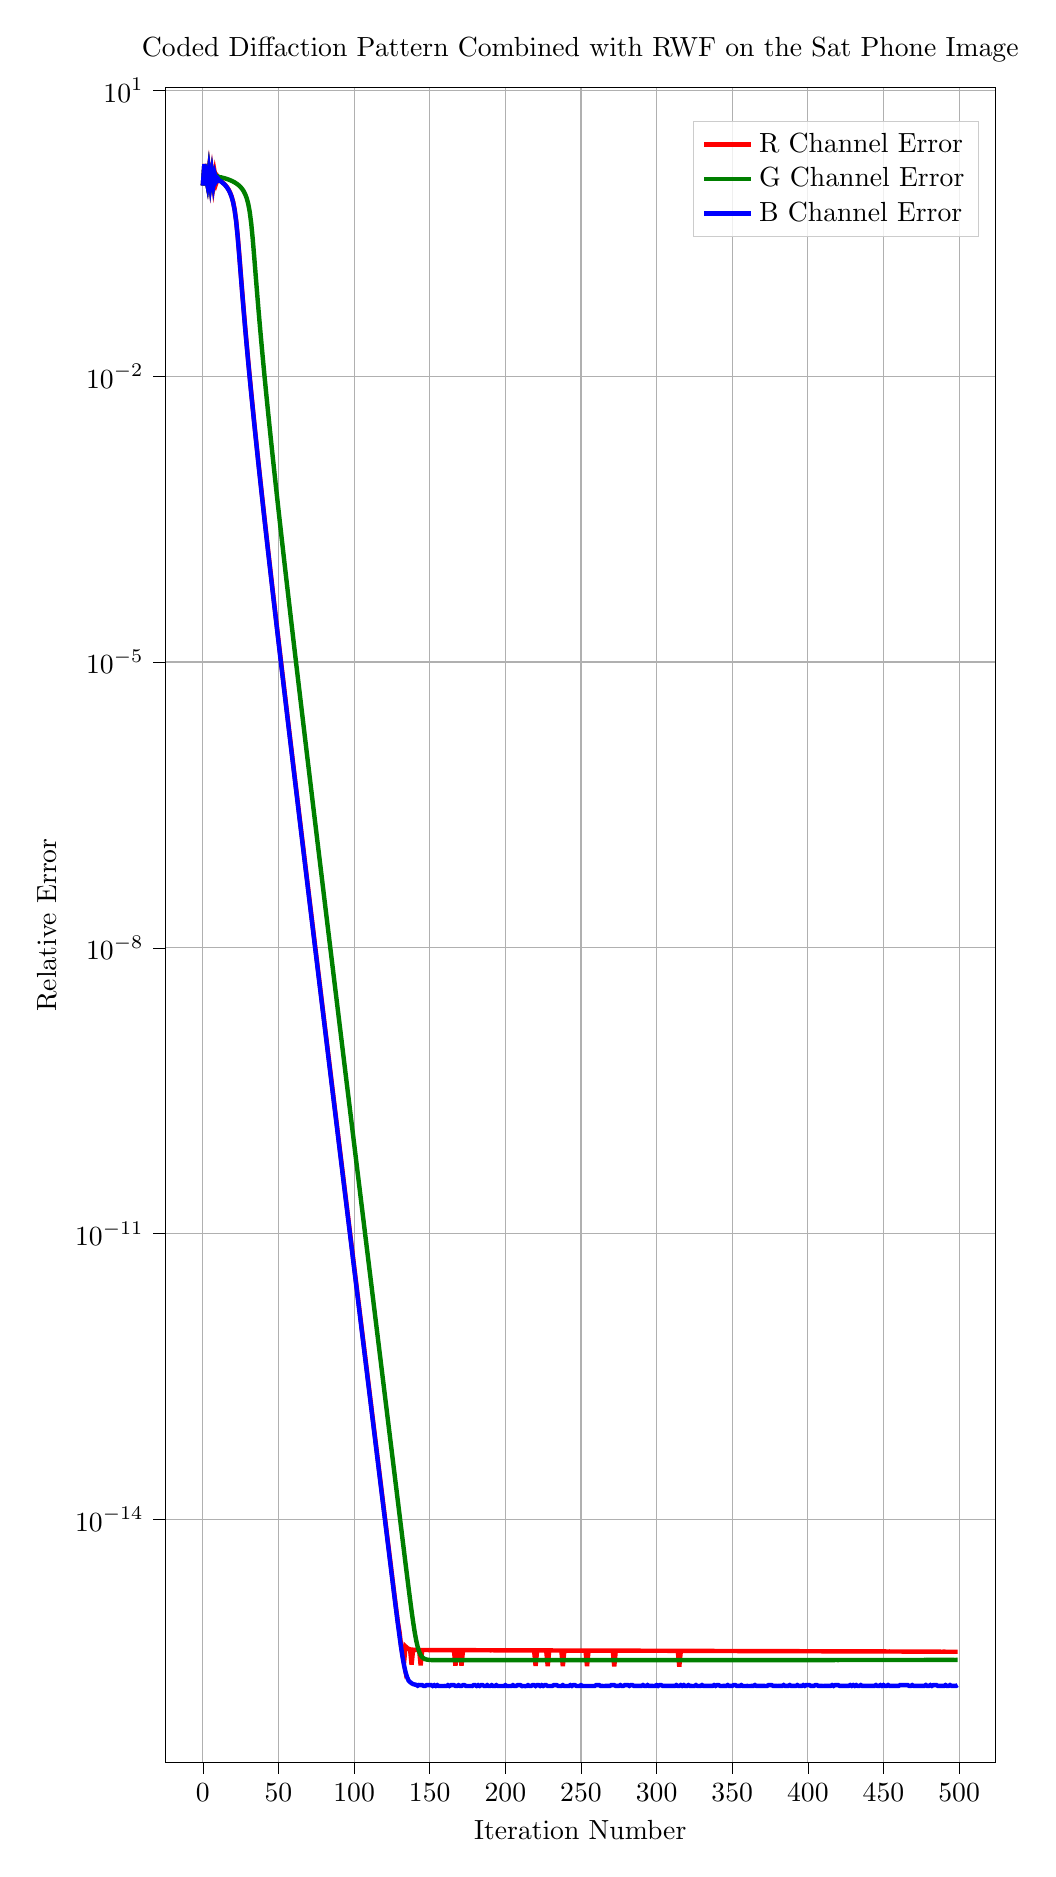
\begin{tikzpicture}

  \definecolor{darkgray176}{RGB}{176,176,176}
  \definecolor{green01270}{RGB}{0,127,0}
  \definecolor{lightgray204}{RGB}{204,204,204}
  
  \begin{axis}[
    width = 1.0\textwidth,
    height = 65em,
  legend cell align={left},
  legend style={fill opacity=0.8, draw opacity=1, text opacity=1, draw=lightgray204},
  log basis y={10},
  tick align=outside,
  tick pos=left,
  title={Coded Diffaction Pattern Combined with 
   \ac{RWF} on the Sat Phone Image},
  x grid style={darkgray176},
  xlabel={Iteration Number},
  xmajorgrids,
  xmin=-24.95, xmax=523.95,
  xtick style={color=black},
  y grid style={darkgray176},
  ylabel={Relative Error},
  ymajorgrids,
  ymin=2.83381160988222e-17, ymax=10.6136402279401,
  ymode=log,
  ytick style={color=black},
  ytick={1e-20,1e-17,1e-14,1e-11,1e-08,1e-05,0.01,10,10000,10000000},
  yticklabels={
    \(\displaystyle {10^{-20}}\),
    \(\displaystyle {10^{-17}}\),
    \(\displaystyle {10^{-14}}\),
    \(\displaystyle {10^{-11}}\),
    \(\displaystyle {10^{-8}}\),
    \(\displaystyle {10^{-5}}\),
    \(\displaystyle {10^{-2}}\),
    \(\displaystyle {10^{1}}\),
    \(\displaystyle {10^{4}}\),
    \(\displaystyle {10^{7}}\)
  }
  ]
  \addplot [ultra thick, red]
  table {%
  0 1.00074586801071
  1 1.6868218123211
  2 1.25263698079135
  3 1.0297941260358
  4 1.44998443738169
  5 1.03325286813443
  6 1.38143373932664
  7 1.01060775435465
  8 1.32948873788063
  9 1.07917504673713
  10 1.20583713241243
  11 1.1218540079197
  12 1.11807514585236
  13 1.07794845316244
  14 1.047179500889
  15 1.00660985997812
  16 0.962034480921937
  17 0.909222619770717
  18 0.84664577681531
  19 0.770689137363532
  20 0.677395628354106
  21 0.563608771795283
  22 0.43265866217846
  23 0.30197388891175
  24 0.195653330466221
  25 0.123170297729902
  26 0.0777995559739119
  27 0.0498862489956395
  28 0.0325341250828546
  29 0.0215506580200378
  30 0.0144698754386949
  31 0.0098287850135905
  32 0.00674269394697365
  33 0.00466509569519606
  34 0.00325150099504432
  35 0.00228083234276688
  36 0.00160896017282267
  37 0.00114064322000335
  38 0.00081219214547537
  39 0.000580575050824566
  40 0.000416449626829298
  41 0.000299645824476183
  42 0.000216198329048023
  43 0.000156375324409178
  44 0.000113355813261773
  45 8.233406368815e-05
  46 5.99083066317952e-05
  47 4.36603880037577e-05
  48 3.18647960445956e-05
  49 2.32860226391293e-05
  50 1.70366630288625e-05
  51 1.24775489270469e-05
  52 9.14714228227171e-06
  53 6.71140837821246e-06
  54 4.92809326162788e-06
  55 3.62117849972507e-06
  56 2.66255649621059e-06
  57 1.95884800830707e-06
  58 1.44189439269887e-06
  59 1.06188416380572e-06
  60 7.82373433589904e-07
  61 5.76671467373059e-07
  62 4.25212551630552e-07
  63 3.13642016828624e-07
  64 2.31420365263306e-07
  65 1.70803939144795e-07
  66 1.26099684111855e-07
  67 9.31197258372068e-08
  68 6.87818008899853e-08
  69 5.08162818891243e-08
  70 3.7551189374954e-08
  71 2.77543167656993e-08
  72 2.05172192677097e-08
  73 1.51699141364434e-08
  74 1.12181275041365e-08
  75 8.29710489886269e-09
  76 6.13759763910578e-09
  77 4.54080479579081e-09
  78 3.35990549631293e-09
  79 2.48644333974264e-09
  80 1.84028473780023e-09
  81 1.36221074652743e-09
  82 1.00845016277837e-09
  83 7.46644092988935e-10
  84 5.5286642256621e-10
  85 4.09423382174893e-10
  86 3.03228128462486e-10
  87 2.24599827143727e-10
  88 1.66376200853459e-10
  89 1.23257594178601e-10
  90 9.13220796249654e-11
  91 6.76669354867549e-11
  92 5.01435277562912e-11
  93 3.7161225310648e-11
  94 2.75423559902626e-11
  95 2.04149012765201e-11
  96 1.51330980434077e-11
  97 1.1218687729461e-11
  98 8.31743192592556e-12
  99 6.1669263081049e-12
  100 4.57277650814178e-12
  101 3.39095717013062e-12
  102 2.51475181800006e-12
  103 1.86508203442051e-12
  104 1.38334417829077e-12
  105 1.02610437180532e-12
  106 7.61168945345241e-13
  107 5.6467531139434e-13
  108 4.18933735982894e-13
  109 3.10825163694457e-13
  110 2.30629542283852e-13
  111 1.71136588883416e-13
  112 1.26995813222239e-13
  113 9.42463912332864e-14
  114 6.99462309208853e-14
  115 5.19146000532284e-14
  116 3.8533709361001e-14
  117 2.86031352771594e-14
  118 2.12330042368106e-14
  119 1.57630157516163e-14
  120 1.17052336355887e-14
  121 8.69813980933904e-15
  122 6.4642206075213e-15
  123 4.80802951796178e-15
  124 3.58154183674529e-15
  125 2.64703026179247e-15
  126 1.96972828553126e-15
  127 1.46831410786226e-15
  128 1.09797241089379e-15
  129 8.25705922660355e-16
  130 6.64811677349937e-16
  131 4.83686638306805e-16
  132 3.82060449900284e-16
  133 3.12351281986232e-16
  134 4.64885253773733e-16
  135 4.48484180467528e-16
  136 4.39137055954418e-16
  137 4.33746031672154e-16
  138 2.99470889968997e-16
  139 4.29175112170883e-16
  140 4.28096209457351e-16
  141 4.27416508290057e-16
  142 4.27075394175611e-16
  143 4.26733811466308e-16
  144 2.93624854960093e-16
  145 4.26411484890944e-16
  146 4.26358461202747e-16
  147 4.26225611706801e-16
  148 4.260897045337e-16
  149 4.25922226723084e-16
  150 4.2583125751176e-16
  151 4.25726770969525e-16
  152 4.25684324641059e-16
  153 4.25656714323803e-16
  154 4.25510958825661e-16
  155 4.25250850481161e-16
  156 4.25251054426769e-16
  157 4.25237310805219e-16
  158 4.25229961841113e-16
  159 4.25266673601401e-16
  160 4.25219680665699e-16
  161 4.25192625926213e-16
  162 4.25176121538865e-16
  163 4.25108524566756e-16
  164 4.25038904162001e-16
  165 4.24896364465815e-16
  166 4.24721806789244e-16
  167 2.91936151355279e-16
  168 4.24770003014642e-16
  169 4.24732359283561e-16
  170 4.24737286543845e-16
  171 2.91829608256277e-16
  172 4.24664440786626e-16
  173 4.24601350880379e-16
  174 4.24477693075121e-16
  175 4.24398670435486e-16
  176 4.24366270701617e-16
  177 4.24258645935244e-16
  178 4.24184421164326e-16
  179 4.24166120034132e-16
  180 4.24159779511216e-16
  181 4.24079345312507e-16
  182 4.23825109591521e-16
  183 4.23814314129036e-16
  184 4.23649821984426e-16
  185 4.23633925359074e-16
  186 4.23595639318322e-16
  187 4.23582284540878e-16
  188 4.23610545926648e-16
  189 4.23437476937517e-16
  190 4.23336548364745e-16
  191 4.23352525096893e-16
  192 4.23356200061498e-16
  193 4.23310610562191e-16
  194 4.23193110176739e-16
  195 4.23209988588763e-16
  196 4.23264716797528e-16
  197 4.23240599296623e-16
  198 4.23166207969337e-16
  199 4.23165247644657e-16
  200 4.23030339110221e-16
  201 4.23001036389334e-16
  202 4.23042144010159e-16
  203 4.23024018055896e-16
  204 4.2294556169524e-16
  205 4.22900850109556e-16
  206 4.22884345961006e-16
  207 4.22949285665332e-16
  208 4.22803691348738e-16
  209 4.22819850956568e-16
  210 4.22773523718597e-16
  211 4.22666504812091e-16
  212 4.22673662473957e-16
  213 4.22536037170173e-16
  214 4.22462157614407e-16
  215 4.22352913520773e-16
  216 4.22413936978623e-16
  217 4.22418586022364e-16
  218 4.22365512922556e-16
  219 4.22372885029553e-16
  220 2.89845050778311e-16
  221 4.22411364301089e-16
  222 4.22267280370411e-16
  223 4.22326882079787e-16
  224 4.22198751505318e-16
  225 4.22062009044018e-16
  226 4.22044354996725e-16
  227 4.21882045000641e-16
  228 2.89048423313315e-16
  229 4.21590285850445e-16
  230 4.2159069585085e-16
  231 4.21571982365656e-16
  232 4.21486820231697e-16
  233 4.21458173839231e-16
  234 4.21294957486066e-16
  235 4.21010217209292e-16
  236 4.2098455691124e-16
  237 4.20975440858488e-16
  238 2.8842343770491e-16
  239 4.20890512654548e-16
  240 4.20737415924818e-16
  241 4.20802207146944e-16
  242 4.20681497065523e-16
  243 4.20697486339362e-16
  244 4.20561718279253e-16
  245 4.2067078025595e-16
  246 4.20589308445475e-16
  247 4.20508746110198e-16
  248 4.2041189792177e-16
  249 4.20397856592924e-16
  250 4.20531718543712e-16
  251 4.20432297846126e-16
  252 4.20512694596265e-16
  253 4.20473106971795e-16
  254 2.87903126330443e-16
  255 4.20494152814552e-16
  256 4.20393503434766e-16
  257 4.20212662252659e-16
  258 4.20135733989428e-16
  259 4.2019280440419e-16
  260 4.20095282423914e-16
  261 4.20055002362523e-16
  262 4.20070837617534e-16
  263 4.19942742149722e-16
  264 4.19982523797909e-16
  265 4.19895737603822e-16
  266 4.1983640709283e-16
  267 4.19727503460881e-16
  268 4.19676494442247e-16
  269 4.19612700237051e-16
  270 4.19659806572781e-16
  271 4.19638698415494e-16
  272 2.87202541579306e-16
  273 4.19538037900876e-16
  274 4.19361367340814e-16
  275 4.19295817819431e-16
  276 4.19277132411717e-16
  277 4.19335417802141e-16
  278 4.19285381265034e-16
  279 4.19253256581385e-16
  280 4.19345508891688e-16
  281 4.19416762077471e-16
  282 4.19277045513254e-16
  283 4.19246616593335e-16
  284 4.19175438542979e-16
  285 4.19042926606161e-16
  286 4.19060104087977e-16
  287 4.19077193575256e-16
  288 4.19040646274742e-16
  289 4.1905782099366e-16
  290 4.18943464412089e-16
  291 4.18888577650373e-16
  292 4.18851038949172e-16
  293 4.18867390428279e-16
  294 4.18814893337822e-16
  295 4.18645248597065e-16
  296 4.18633321809346e-16
  297 4.18673509150342e-16
  298 4.18672144807409e-16
  299 4.18525277990184e-16
  300 4.18492011551843e-16
  301 4.18469947498256e-16
  302 4.18442746323308e-16
  303 4.18381584997844e-16
  304 4.18336031441103e-16
  305 4.18344359262212e-16
  306 4.18311409178216e-16
  307 4.18276261544244e-16
  308 4.18159118242134e-16
  309 4.18034878990327e-16
  310 4.18027908533966e-16
  311 4.17872213645833e-16
  312 4.17818682672352e-16
  313 4.17699460564266e-16
  314 4.17709958209621e-16
  315 2.85567831680655e-16
  316 4.17477187839178e-16
  317 4.17465557546363e-16
  318 4.17444111264102e-16
  319 4.17412354205297e-16
  320 4.17371213560738e-16
  321 4.17192313235505e-16
  322 4.1708215536535e-16
  323 4.17108467459851e-16
  324 4.17112328484713e-16
  325 4.16966107901452e-16
  326 4.17064555402633e-16
  327 4.17008845670969e-16
  328 4.16982225928534e-16
  329 4.17046823154292e-16
  330 4.16949884779095e-16
  331 4.16828137719309e-16
  332 4.16773444345861e-16
  333 4.16677599451257e-16
  334 4.16638318180451e-16
  335 4.16648259811438e-16
  336 4.16564769765849e-16
  337 4.16553319171448e-16
  338 4.16501717382018e-16
  339 4.16374737803361e-16
  340 4.16335172205193e-16
  341 4.16227123216212e-16
  342 4.16220034387734e-16
  343 4.16230487383661e-16
  344 4.160790524907e-16
  345 4.16011134397701e-16
  346 4.16069942609371e-16
  347 4.16201313531252e-16
  348 4.16027836282568e-16
  349 4.15920356250086e-16
  350 4.15844335896428e-16
  351 4.15884426495433e-16
  352 4.15852580905102e-16
  353 4.15812123685458e-16
  354 4.15689411123669e-16
  355 4.15580525705744e-16
  356 4.15569695632212e-16
  357 4.15560526326505e-16
  358 4.15436586496643e-16
  359 4.15289211805025e-16
  360 4.15233199199643e-16
  361 4.15218137113165e-16
  362 4.15295536185405e-16
  363 4.15110531536646e-16
  364 4.15109322421726e-16
  365 4.15069413527332e-16
  366 4.14964677179374e-16
  367 4.14981097573032e-16
  368 4.14973192639816e-16
  369 4.14895885864369e-16
  370 4.14979784784296e-16
  371 4.14917257597037e-16
  372 4.14838221093916e-16
  373 4.14850004966114e-16
  374 4.14768704736629e-16
  375 4.14737644931654e-16
  376 4.14715594620727e-16
  377 4.14677093514847e-16
  378 4.14517229523159e-16
  379 4.14585286154463e-16
  380 4.14514611488623e-16
  381 4.14391582279151e-16
  382 4.14266731060818e-16
  383 4.14266937364996e-16
  384 4.14226504621985e-16
  385 4.14215279294068e-16
  386 4.14204378600603e-16
  387 4.14111827722369e-16
  388 4.14107833624011e-16
  389 4.14158565122272e-16
  390 4.14148752063313e-16
  391 4.14094579425872e-16
  392 4.14076983339476e-16
  393 4.14002925435668e-16
  394 4.14040109065193e-16
  395 4.13918868924392e-16
  396 4.13956932264529e-16
  397 4.13920655360728e-16
  398 4.13893079442743e-16
  399 4.13910834465044e-16
  400 4.13699658962402e-16
  401 4.1372669197426e-16
  402 4.13664636710962e-16
  403 4.13679639102129e-16
  404 4.13643545638207e-16
  405 4.13515210720449e-16
  406 4.13518585086725e-16
  407 4.13401741781872e-16
  408 4.13372399049731e-16
  409 4.13247533969814e-16
  410 4.13241396223684e-16
  411 4.13183894789042e-16
  412 4.13055149201559e-16
  413 4.1302600516945e-16
  414 4.12943718333426e-16
  415 4.12894490014726e-16
  416 4.12910175820661e-16
  417 4.12865238775837e-16
  418 4.12798667297487e-16
  419 4.12763565664593e-16
  420 4.12832998064044e-16
  421 4.12776684237653e-16
  422 4.12758509163277e-16
  423 4.12632469336064e-16
  424 4.12568041868654e-16
  425 4.12523287477612e-16
  426 4.12320976325633e-16
  427 4.12355476360448e-16
  428 4.12384168859614e-16
  429 4.12451361318675e-16
  430 4.12434159192227e-16
  431 4.12480969060586e-16
  432 4.12469327872186e-16
  433 4.12444005649333e-16
  434 4.1234703262647e-16
  435 4.12237674555291e-16
  436 4.12233581892311e-16
  437 4.12240946016965e-16
  438 4.12164564009071e-16
  439 4.12091775402375e-16
  440 4.1202731188181e-16
  441 4.12112635106932e-16
  442 4.12034654910005e-16
  443 4.11982130131583e-16
  444 4.1196469300621e-16
  445 4.1183817000927e-16
  446 4.11748620298523e-16
  447 4.11746541930157e-16
  448 4.11845579711999e-16
  449 4.1176722961832e-16
  450 4.11693725238666e-16
  451 4.11515514886485e-16
  452 4.11460156895828e-16
  453 4.11427476216318e-16
  454 4.11490525774214e-16
  455 4.11381173614289e-16
  456 4.11267583705838e-16
  457 4.11204696909894e-16
  458 4.11091700137919e-16
  459 4.10963269905058e-16
  460 4.10973413677647e-16
  461 4.10880718284353e-16
  462 4.10770201220359e-16
  463 4.10634151769792e-16
  464 4.10604984382077e-16
  465 4.10553287153279e-16
  466 4.10520036396503e-16
  467 4.10447695568083e-16
  468 4.10354240856264e-16
  469 4.10237997691248e-16
  470 4.10221528413831e-16
  471 4.10111808363946e-16
  472 4.10113082572705e-16
  473 4.09971921495496e-16
  474 4.10016605241481e-16
  475 4.10046313134055e-16
  476 4.10003603840501e-16
  477 4.09925823116011e-16
  478 4.09757343315601e-16
  479 4.09619156713499e-16
  480 4.0961406834267e-16
  481 4.09538864892822e-16
  482 4.09399341170717e-16
  483 4.09394355602967e-16
  484 4.0933987962115e-16
  485 4.09286180235633e-16
  486 4.09274456314222e-16
  487 4.091268203392e-16
  488 4.08979248566792e-16
  489 4.08997720832156e-16
  490 4.09071620582006e-16
  491 4.08988080579888e-16
  492 4.08979567728346e-16
  493 4.0884772073542e-16
  494 4.08950784047632e-16
  495 4.08904621173151e-16
  496 4.08751311245635e-16
  497 4.08792782323396e-16
  498 4.08733227930995e-16
  499 4.08699300895397e-16
  };
  \addlegendentry{R Channel Error}
  \addplot [ultra thick, green01270]
  table {%
  0 1.00095014178353
  1 1.67087098235772
  2 1.24701982732465
  3 1.0285957768824
  4 1.43005915083823
  5 1.03934989258295
  6 1.36092052523279
  7 1.05290484740549
  8 1.31960983473312
  9 1.22068167724216
  10 1.24789297426872
  11 1.22715156893451
  12 1.22201751932254
  13 1.20974782471849
  14 1.19867753703325
  15 1.18570964620883
  16 1.1719402192376
  17 1.15684077135662
  18 1.1404346211364
  19 1.12249817654727
  20 1.10281892272665
  21 1.08109684081357
  22 1.05694007526273
  23 1.02980744285062
  24 0.99898198660717
  25 0.963466069176554
  26 0.921902680342581
  27 0.872364078964801
  28 0.812087103832484
  29 0.737307099010209
  30 0.643596843160304
  31 0.528459734581391
  32 0.39788574277044
  33 0.272670531274854
  34 0.175374334390435
  35 0.11071046527583
  36 0.0704027173053537
  37 0.0454782048487208
  38 0.0298614655119067
  39 0.0198990763930201
  40 0.0134302390322869
  41 0.00916339544657805
  42 0.00631056019556702
  43 0.00438084116505697
  44 0.00306238561256629
  45 0.00215372817663484
  46 0.00152275363612124
  47 0.0010816940533992
  48 0.00077158223335908
  49 0.000552410535239181
  50 0.000396797318288127
  51 0.000285857220574559
  52 0.000206475316682028
  53 0.000149487948174554
  54 0.000108456946824746
  55 7.88365565734046e-05
  56 5.74028331713698e-05
  57 4.18600685643528e-05
  58 3.05675850037058e-05
  59 2.23489846795012e-05
  60 1.63582659121828e-05
  61 1.19854010192503e-05
  62 8.78945313410378e-06
  63 6.45101117168508e-06
  64 4.73824049644588e-06
  65 3.48257180793689e-06
  66 2.56123977264853e-06
  67 1.88470732994981e-06
  68 1.38758630208899e-06
  69 1.0220675870321e-06
  70 7.53157628613565e-07
  71 5.55218203885961e-07
  72 4.09448750485722e-07
  73 3.02051729000214e-07
  74 2.22893888638312e-07
  75 1.64528183532376e-07
  76 1.21478379116748e-07
  77 8.97152630766993e-08
  78 6.6272788358644e-08
  79 4.89665282643175e-08
  80 3.61870155794313e-08
  81 2.67479425884043e-08
  82 1.97745874306172e-08
  83 1.46217592703662e-08
  84 1.08134203931308e-08
  85 7.99823700117436e-09
  86 5.91684175010212e-09
  87 4.37771218887007e-09
  88 3.23939077138917e-09
  89 2.39737461614384e-09
  90 1.77444539689504e-09
  91 1.31353449737508e-09
  92 9.72457271945529e-10
  93 7.20025734829892e-10
  94 5.33178136475269e-10
  95 3.94858930922832e-10
  96 2.92452624611932e-10
  97 2.16626563251246e-10
  98 1.60475713345908e-10
  99 1.18890515861927e-10
  100 8.80895400481113e-11
  101 6.52739234308485e-11
  102 4.83718173437908e-11
  103 3.58493699426836e-11
  104 2.65708992290445e-11
  105 1.96954452500528e-11
  106 1.46002210579683e-11
  107 1.08239663967834e-11
  108 8.02502043306317e-12
  109 5.95028702563256e-12
  110 4.41226051590749e-12
  111 3.27201458674897e-12
  112 2.426607955186e-12
  113 1.79975675426141e-12
  114 1.33492610280747e-12
  115 9.90214648073855e-13
  116 7.34564110345244e-13
  117 5.44951645500215e-13
  118 4.04309194548874e-13
  119 2.99982772104168e-13
  120 2.22589941987612e-13
  121 1.65173682300546e-13
  122 1.22575303555755e-13
  123 9.09683757718072e-14
  124 6.75156013010782e-14
  125 5.01123352586085e-14
  126 3.71972306408894e-14
  127 2.76126898263935e-14
  128 2.04993486041685e-14
  129 1.52200162116e-14
  130 1.13191741494884e-14
  131 8.39380013075911e-15
  132 6.23636899303264e-15
  133 4.63604237741327e-15
  134 3.4495909535446e-15
  135 2.5711414393115e-15
  136 1.92222825056771e-15
  137 1.44473662596564e-15
  138 1.09573412981502e-15
  139 8.43979557939711e-16
  140 6.65490219689436e-16
  141 5.4270055865108e-16
  142 4.61217831470621e-16
  143 4.09260244245718e-16
  144 3.77596832278813e-16
  145 3.58801036128357e-16
  146 3.47928035230066e-16
  147 3.4169393976515e-16
  148 3.38220793631162e-16
  149 3.36203376467721e-16
  150 3.35166184892723e-16
  151 3.34479329679099e-16
  152 3.34127817088468e-16
  153 3.33917269534378e-16
  154 3.33849945042583e-16
  155 3.33676088740873e-16
  156 3.33706988427376e-16
  157 3.33679813901632e-16
  158 3.33663450083346e-16
  159 3.33646076290167e-16
  160 3.33645030651952e-16
  161 3.33568397426375e-16
  162 3.33585799144145e-16
  163 3.33554873542117e-16
  164 3.33445048695844e-16
  165 3.33507943036892e-16
  166 3.33377095921546e-16
  167 3.33408666449998e-16
  168 3.3336500650198e-16
  169 3.33392358110428e-16
  170 3.33343022763487e-16
  171 3.33376140274012e-16
  172 3.33476685995579e-16
  173 3.33438343938873e-16
  174 3.33424056685638e-16
  175 3.3338157201302e-16
  176 3.33397869997209e-16
  177 3.33415219354136e-16
  178 3.33482159423876e-16
  179 3.33454217459931e-16
  180 3.33504587135935e-16
  181 3.33529865647318e-16
  182 3.33546036101442e-16
  183 3.3354383056538e-16
  184 3.33604531097818e-16
  185 3.33691402351458e-16
  186 3.33667562162265e-16
  187 3.33634273646391e-16
  188 3.33601389803803e-16
  189 3.33657030049249e-16
  190 3.33643332783218e-16
  191 3.33568326568692e-16
  192 3.33567101100773e-16
  193 3.336041453608e-16
  194 3.33530657557776e-16
  195 3.33609679070763e-16
  196 3.33593195914397e-16
  197 3.33601337190567e-16
  198 3.33605680461853e-16
  199 3.33563339697989e-16
  200 3.33518546056358e-16
  201 3.33545710633547e-16
  202 3.33494343395991e-16
  203 3.33519510393333e-16
  204 3.33542115121717e-16
  205 3.33601243043252e-16
  206 3.33642211149316e-16
  207 3.33646904185913e-16
  208 3.33596416018085e-16
  209 3.336592455957e-16
  210 3.33656537955517e-16
  211 3.33695098603899e-16
  212 3.3365043281671e-16
  213 3.3361285204822e-16
  214 3.33726594550195e-16
  215 3.3370134763644e-16
  216 3.33708260805353e-16
  217 3.33763156670421e-16
  218 3.33811610900387e-16
  219 3.33820567761685e-16
  220 3.33825020290369e-16
  221 3.33858126729864e-16
  222 3.33890227791992e-16
  223 3.33878048204808e-16
  224 3.3388406349943e-16
  225 3.33855327365372e-16
  226 3.33822693286105e-16
  227 3.33758641132821e-16
  228 3.33779331104508e-16
  229 3.33828231974304e-16
  230 3.33818787437261e-16
  231 3.3374980753776e-16
  232 3.33816806843774e-16
  233 3.338126413109e-16
  234 3.33695607634297e-16
  235 3.33589081098575e-16
  236 3.33517955266029e-16
  237 3.33577720962249e-16
  238 3.33750304368629e-16
  239 3.33701675374811e-16
  240 3.3370940741206e-16
  241 3.33707649531792e-16
  242 3.33639781240105e-16
  243 3.33646967948197e-16
  244 3.3355273866421e-16
  245 3.3357462905209e-16
  246 3.33565346534189e-16
  247 3.33618798244268e-16
  248 3.33594731703782e-16
  249 3.33622277658175e-16
  250 3.33630368084826e-16
  251 3.33621791853507e-16
  252 3.3363871572623e-16
  253 3.3374557776666e-16
  254 3.33778154225118e-16
  255 3.33734705335241e-16
  256 3.33721823116952e-16
  257 3.33697105067816e-16
  258 3.33669874229618e-16
  259 3.33534613352197e-16
  260 3.33622426199177e-16
  261 3.33584194376128e-16
  262 3.3364310212979e-16
  263 3.33583128675121e-16
  264 3.33664174839199e-16
  265 3.33629376291543e-16
  266 3.33567806287925e-16
  267 3.33530248715284e-16
  268 3.33645832646662e-16
  269 3.33572915557088e-16
  270 3.33534382716134e-16
  271 3.33592671192308e-16
  272 3.33569583342017e-16
  273 3.33673049905508e-16
  274 3.33693764221594e-16
  275 3.33626232264016e-16
  276 3.33614512397173e-16
  277 3.3361976245838e-16
  278 3.33701440215676e-16
  279 3.33608646903111e-16
  280 3.337267185519e-16
  281 3.33767600838994e-16
  282 3.33761990474158e-16
  283 3.3385517292799e-16
  284 3.33861865855299e-16
  285 3.33808839094087e-16
  286 3.33808029635283e-16
  287 3.33801077960735e-16
  288 3.33817818977493e-16
  289 3.3390796697474e-16
  290 3.33889345567866e-16
  291 3.33902680377937e-16
  292 3.33872832894937e-16
  293 3.33954151982716e-16
  294 3.3393563706384e-16
  295 3.33944209773982e-16
  296 3.34024869242581e-16
  297 3.33986836223098e-16
  298 3.33949231612461e-16
  299 3.33947086673943e-16
  300 3.3402485554027e-16
  301 3.34031753273747e-16
  302 3.34086561129894e-16
  303 3.33980943838311e-16
  304 3.34009083499973e-16
  305 3.33992992786167e-16
  306 3.33974907965725e-16
  307 3.34017944249183e-16
  308 3.34043331094718e-16
  309 3.34084098244389e-16
  310 3.33991352893198e-16
  311 3.34015780777977e-16
  312 3.34082292292702e-16
  313 3.33962876854236e-16
  314 3.3397074278059e-16
  315 3.34057273900923e-16
  316 3.34167354429282e-16
  317 3.34141798849943e-16
  318 3.34214716363063e-16
  319 3.34095686125334e-16
  320 3.34153854767289e-16
  321 3.34235185077966e-16
  322 3.34256341449085e-16
  323 3.34244764167619e-16
  324 3.34283127027395e-16
  325 3.34144885381958e-16
  326 3.34244420485725e-16
  327 3.34234435018906e-16
  328 3.34294010712503e-16
  329 3.34246573495697e-16
  330 3.34283404921332e-16
  331 3.34207286695158e-16
  332 3.3420017088116e-16
  333 3.34179204831091e-16
  334 3.34160440082576e-16
  335 3.34162193008357e-16
  336 3.34048588312652e-16
  337 3.34113703680879e-16
  338 3.34106762064268e-16
  339 3.34067681212378e-16
  340 3.3406736679503e-16
  341 3.34024820348246e-16
  342 3.34087022901759e-16
  343 3.34013855363036e-16
  344 3.34036294279771e-16
  345 3.34142495767134e-16
  346 3.34078164605559e-16
  347 3.34065801350673e-16
  348 3.34136947064809e-16
  349 3.34106569859357e-16
  350 3.34116201359643e-16
  351 3.34077098407454e-16
  352 3.34046689686099e-16
  353 3.34070168367921e-16
  354 3.34167350698262e-16
  355 3.34096806629869e-16
  356 3.34150719249428e-16
  357 3.34189137125842e-16
  358 3.34182858318805e-16
  359 3.34180281138215e-16
  360 3.34204379113828e-16
  361 3.34210494848848e-16
  362 3.34177682608993e-16
  363 3.34226680976175e-16
  364 3.34216027544247e-16
  365 3.34218729263814e-16
  366 3.34177850916428e-16
  367 3.34291997069252e-16
  368 3.34172482665574e-16
  369 3.34186913267183e-16
  370 3.34239804613244e-16
  371 3.34137389283514e-16
  372 3.34095533668589e-16
  373 3.34241330925594e-16
  374 3.34183546089406e-16
  375 3.34237523286415e-16
  376 3.34256925056535e-16
  377 3.34221330282841e-16
  378 3.3433605985497e-16
  379 3.34176993999912e-16
  380 3.34205817279403e-16
  381 3.34187447870572e-16
  382 3.34137799392659e-16
  383 3.34078765734149e-16
  384 3.34114797968884e-16
  385 3.34039843256429e-16
  386 3.34104893293893e-16
  387 3.34101249844516e-16
  388 3.3411994466679e-16
  389 3.341563988543e-16
  390 3.34198606747565e-16
  391 3.34240880937177e-16
  392 3.34158929663877e-16
  393 3.34166443139491e-16
  394 3.34152457489867e-16
  395 3.34126275238058e-16
  396 3.34165656120993e-16
  397 3.34206951815292e-16
  398 3.34139372638278e-16
  399 3.34170769873567e-16
  400 3.34083086657007e-16
  401 3.34299651372013e-16
  402 3.34234507136924e-16
  403 3.3422259027037e-16
  404 3.34098466419398e-16
  405 3.3426861732354e-16
  406 3.34296265717091e-16
  407 3.34333341405217e-16
  408 3.34359936744151e-16
  409 3.34341439031271e-16
  410 3.34338835315406e-16
  411 3.3434988400614e-16
  412 3.34368269084514e-16
  413 3.34321313346174e-16
  414 3.34431592745647e-16
  415 3.34379251276643e-16
  416 3.34476257063671e-16
  417 3.34389035957649e-16
  418 3.34527608032963e-16
  419 3.34508774196903e-16
  420 3.34469497599524e-16
  421 3.34548549199819e-16
  422 3.34532472699149e-16
  423 3.34509435717409e-16
  424 3.34595875741262e-16
  425 3.34595086728188e-16
  426 3.3462338658542e-16
  427 3.3467044901663e-16
  428 3.34622290179082e-16
  429 3.34532474415887e-16
  430 3.34540067273212e-16
  431 3.34536236884842e-16
  432 3.34565206813558e-16
  433 3.3454314755653e-16
  434 3.34584824689733e-16
  435 3.34578414681004e-16
  436 3.34657716940858e-16
  437 3.34649308343991e-16
  438 3.34687920861748e-16
  439 3.34641455793274e-16
  440 3.34695856922213e-16
  441 3.34671487350011e-16
  442 3.34709998191974e-16
  443 3.34681882287393e-16
  444 3.34674911869581e-16
  445 3.3475355013855e-16
  446 3.34766366580565e-16
  447 3.34773255115235e-16
  448 3.34746958272597e-16
  449 3.34734419927595e-16
  450 3.34795580015962e-16
  451 3.34843904802248e-16
  452 3.34907062458698e-16
  453 3.34920209309721e-16
  454 3.34896912580203e-16
  455 3.34926748569523e-16
  456 3.34923340685701e-16
  457 3.34973197629033e-16
  458 3.34958720589046e-16
  459 3.34894673013418e-16
  460 3.34838766946044e-16
  461 3.34873005840257e-16
  462 3.34809692709389e-16
  463 3.34843473118091e-16
  464 3.34939039409433e-16
  465 3.34945683116295e-16
  466 3.34995313168294e-16
  467 3.34828875928718e-16
  468 3.34837789068694e-16
  469 3.34861124661231e-16
  470 3.34912303752933e-16
  471 3.34877876835466e-16
  472 3.34945038751919e-16
  473 3.34998044096807e-16
  474 3.34967193261681e-16
  475 3.34956887033532e-16
  476 3.35023639700057e-16
  477 3.35074439517428e-16
  478 3.35064632701605e-16
  479 3.35134713845526e-16
  480 3.35173421006294e-16
  481 3.35140100898234e-16
  482 3.35200775453097e-16
  483 3.35162056075333e-16
  484 3.35132882855581e-16
  485 3.35134158972572e-16
  486 3.35157897605275e-16
  487 3.35225604793175e-16
  488 3.35188851564576e-16
  489 3.3521757504019e-16
  490 3.35196622675145e-16
  491 3.35242347355305e-16
  492 3.35211115472e-16
  493 3.35245133978469e-16
  494 3.35149820550809e-16
  495 3.35227506555142e-16
  496 3.35204878668292e-16
  497 3.35047552730695e-16
  498 3.35092808145873e-16
  499 3.35215807069823e-16
  };
  \addlegendentry{G Channel Error}
  \addplot [ultra thick, blue]
  table {%
  0 1.00080892856594
  1 1.67873881270839
  2 1.2472031771211
  3 1.02924823006483
  4 1.43248515430483
  5 1.03158624427673
  6 1.36765936084978
  7 1.02020196660541
  8 1.29222872345673
  9 1.11613644570851
  10 1.1798475510341
  11 1.11954314754296
  12 1.10799714087412
  13 1.0710595563865
  14 1.0392045404828
  15 0.999085436588158
  16 0.954406624516564
  17 0.901578895564351
  18 0.838806629473497
  19 0.762432895804866
  20 0.66834166106848
  21 0.553527992383412
  22 0.422099508368368
  23 0.292483839828798
  24 0.188745431153266
  25 0.118728731781192
  26 0.0750301470845583
  27 0.0481512140012844
  28 0.0314260297381783
  29 0.020827993606456
  30 0.013988994675338
  31 0.00950304937097007
  32 0.00651867475024762
  33 0.00450907929569475
  34 0.00314170733062904
  35 0.0022028893688406
  36 0.00155322691613581
  37 0.00110054965959159
  38 0.000783205076444335
  39 0.00055953078384845
  40 0.000401119344178461
  41 0.000288446452117461
  42 0.000207997602643454
  43 0.000150358793751799
  44 0.000108934732809625
  45 7.90811070332111e-05
  46 5.75122550212235e-05
  47 4.18939425884498e-05
  48 3.05615598127068e-05
  49 2.23239460230414e-05
  50 1.63260807651429e-05
  51 1.19524997518686e-05
  52 8.75904919765158e-06
  53 6.42446447319578e-06
  54 4.71588482414727e-06
  55 3.46420877676066e-06
  56 2.54642692426297e-06
  57 1.8729205382033e-06
  58 1.37830654656798e-06
  59 1.01482313723793e-06
  60 7.47540700139344e-07
  61 5.5088763804428e-07
  62 4.06125592666152e-07
  63 2.99511695013812e-07
  64 2.20958948044785e-07
  65 1.6305843236092e-07
  66 1.2036475411439e-07
  67 8.88732970389446e-08
  68 6.56374153947832e-08
  69 4.84878531812418e-08
  70 3.58269222848632e-08
  71 2.64774077915556e-08
  72 1.95715731303943e-08
  73 1.44695719316542e-08
  74 1.06994414371181e-08
  75 7.91294565637911e-09
  76 5.85306620523219e-09
  77 4.33005781180547e-09
  78 3.20380489967679e-09
  79 2.37081619702176e-09
  80 1.75463480067081e-09
  81 1.2987644427478e-09
  82 9.61450185571672e-10
  83 7.11826316130198e-10
  84 5.27072550976203e-10
  85 3.9031410864668e-10
  86 2.89070711597291e-10
  87 2.14110778838718e-10
  88 1.5860477945281e-10
  89 1.1749952136321e-10
  90 8.70556335536093e-11
  91 6.45056206505107e-11
  92 4.78010163021296e-11
  93 3.54253916741832e-11
  94 2.62560420618318e-11
  95 1.94616694469356e-11
  96 1.44266788832515e-11
  97 1.06951611012581e-11
  98 7.92943516636916e-12
  99 5.87936575921749e-12
  100 4.35964719246802e-12
  101 3.23298869189064e-12
  102 2.39766491349688e-12
  103 1.77829420386868e-12
  104 1.31901288550664e-12
  105 9.78417543076551e-13
  106 7.25819511087685e-13
  107 5.38470421955999e-13
  108 3.99506162998974e-13
  109 2.96423627714501e-13
  110 2.19952602526785e-13
  111 1.6321982719279e-13
  112 1.21127774426741e-13
  113 8.98959812271781e-14
  114 6.67211406915638e-14
  115 4.95236938804666e-14
  116 3.67610147703692e-14
  117 2.72888300940018e-14
  118 2.02588210792476e-14
  119 1.50408281961414e-14
  120 1.11676327014844e-14
  121 8.29258239775334e-15
  122 6.15847199090643e-15
  123 4.57437658333982e-15
  124 3.39880389596557e-15
  125 2.52653918112593e-15
  126 1.87978121496335e-15
  127 1.40127586721064e-15
  128 1.04800581908507e-15
  129 7.87111180217239e-16
  130 5.98050799206009e-16
  131 4.59653492767806e-16
  132 3.62375452363479e-16
  133 2.9516305370331e-16
  134 2.50445192475335e-16
  135 2.21712894364279e-16
  136 2.03996091796078e-16
  137 1.96675332831235e-16
  138 1.90640229835532e-16
  139 1.87213892663212e-16
  140 1.85086776509335e-16
  141 1.83935359768204e-16
  142 1.79787101136216e-16
  143 1.83064906255609e-16
  144 1.82788607381122e-16
  145 1.82545892082025e-16
  146 1.78868404449936e-16
  147 1.78875992180587e-16
  148 1.82481169858002e-16
  149 1.82412731943475e-16
  150 1.82360415988116e-16
  151 1.82483820549433e-16
  152 1.7873432507479e-16
  153 1.82394447143133e-16
  154 1.78686558479852e-16
  155 1.82425967111777e-16
  156 1.78628890057281e-16
  157 1.78580298828536e-16
  158 1.78645731666788e-16
  159 1.78669440624648e-16
  160 1.78755392655619e-16
  161 1.78633498811082e-16
  162 1.82233656881488e-16
  163 1.78489616044021e-16
  164 1.82194668482104e-16
  165 1.82311119092594e-16
  166 1.82329115672755e-16
  167 1.78679451828905e-16
  168 1.78739477899337e-16
  169 1.82283789985665e-16
  170 1.78653736950261e-16
  171 1.78597840197134e-16
  172 1.82283794260825e-16
  173 1.82287681674526e-16
  174 1.78745332438826e-16
  175 1.78669820488425e-16
  176 1.78665597650721e-16
  177 1.78644431862752e-16
  178 1.78474705119993e-16
  179 1.82283871197751e-16
  180 1.82312851508373e-16
  181 1.78698683014382e-16
  182 1.82239194069071e-16
  183 1.7867750490544e-16
  184 1.82311052427581e-16
  185 1.82186699265083e-16
  186 1.78625478728331e-16
  187 1.78675628628196e-16
  188 1.82385553715343e-16
  189 1.78544557741638e-16
  190 1.78520807853018e-16
  191 1.82206587507081e-16
  192 1.78474138292073e-16
  193 1.78488569372676e-16
  194 1.8222922736431e-16
  195 1.78511629292365e-16
  196 1.78634385239336e-16
  197 1.78642688424903e-16
  198 1.78468786581674e-16
  199 1.78532005479403e-16
  200 1.82195204962786e-16
  201 1.7854504676639e-16
  202 1.78439526874108e-16
  203 1.7849048108298e-16
  204 1.78528679056811e-16
  205 1.82198544003848e-16
  206 1.78568403520483e-16
  207 1.78588013584302e-16
  208 1.8214776641337e-16
  209 1.82157168213141e-16
  210 1.82248202699347e-16
  211 1.78306070512943e-16
  212 1.78620451516997e-16
  213 1.78406734458183e-16
  214 1.78475405124204e-16
  215 1.8222983013077e-16
  216 1.78783561203914e-16
  217 1.78694120397978e-16
  218 1.82341211581638e-16
  219 1.82124328244263e-16
  220 1.78469467534906e-16
  221 1.82283749050096e-16
  222 1.82348578860811e-16
  223 1.78561824739437e-16
  224 1.82283562849341e-16
  225 1.78698517703488e-16
  226 1.82215707357897e-16
  227 1.82143991516924e-16
  228 1.78573729028112e-16
  229 1.7861883900186e-16
  230 1.78609274181555e-16
  231 1.78676616533098e-16
  232 1.82408985270492e-16
  233 1.82430383343395e-16
  234 1.82302767568115e-16
  235 1.78642210074748e-16
  236 1.78638617578649e-16
  237 1.78676258663871e-16
  238 1.82326250844685e-16
  239 1.78597269200339e-16
  240 1.78721375612255e-16
  241 1.78688818609153e-16
  242 1.7880400572667e-16
  243 1.82402527383497e-16
  244 1.78800643996874e-16
  245 1.82426528631766e-16
  246 1.8236045430471e-16
  247 1.78639309882169e-16
  248 1.78542869266741e-16
  249 1.78711266028457e-16
  250 1.82238478540258e-16
  251 1.78647692255251e-16
  252 1.78642512874387e-16
  253 1.78596972809618e-16
  254 1.78635294762919e-16
  255 1.78607777281359e-16
  256 1.78676506880452e-16
  257 1.78672884324344e-16
  258 1.78745166877168e-16
  259 1.78628086382454e-16
  260 1.82270510948332e-16
  261 1.82275985946701e-16
  262 1.82440167997843e-16
  263 1.78699644367534e-16
  264 1.78789544127442e-16
  265 1.78617422427144e-16
  266 1.78807073311107e-16
  267 1.78815394831571e-16
  268 1.78824114681758e-16
  269 1.78784142938203e-16
  270 1.82454165994929e-16
  271 1.82406163024165e-16
  272 1.82441069874711e-16
  273 1.78776826191827e-16
  274 1.78796365557684e-16
  275 1.78749505611547e-16
  276 1.82535207540033e-16
  277 1.78809213238773e-16
  278 1.78864694093273e-16
  279 1.82464330300133e-16
  280 1.82385714028789e-16
  281 1.82492327130045e-16
  282 1.78844933575196e-16
  283 1.82609977302331e-16
  284 1.82709256788769e-16
  285 1.78876113588329e-16
  286 1.78927448499167e-16
  287 1.78924310619634e-16
  288 1.789131591603e-16
  289 1.78829695146229e-16
  290 1.78927296547286e-16
  291 1.82658951816086e-16
  292 1.78908639303708e-16
  293 1.78753598763281e-16
  294 1.82696213128206e-16
  295 1.7871402653208e-16
  296 1.78785474873376e-16
  297 1.78796489010013e-16
  298 1.7874291471125e-16
  299 1.78780774683916e-16
  300 1.82433600965721e-16
  301 1.78673316685497e-16
  302 1.82434011233075e-16
  303 1.82558683333806e-16
  304 1.78784180940967e-16
  305 1.78839699159478e-16
  306 1.78745991024742e-16
  307 1.78931432546738e-16
  308 1.78774574524629e-16
  309 1.78935478247541e-16
  310 1.78867390267471e-16
  311 1.78852893614213e-16
  312 1.78886079096974e-16
  313 1.82564534494064e-16
  314 1.78767487092596e-16
  315 1.78747216246893e-16
  316 1.8257945332948e-16
  317 1.7889169974905e-16
  318 1.82609802543642e-16
  319 1.78577797715984e-16
  320 1.78685395817719e-16
  321 1.8250431108295e-16
  322 1.78844194165207e-16
  323 1.78759295783593e-16
  324 1.78703670381898e-16
  325 1.78785364252353e-16
  326 1.82599379580001e-16
  327 1.78776421964403e-16
  328 1.78730263995455e-16
  329 1.7883076440147e-16
  330 1.8264332887032e-16
  331 1.78782717784276e-16
  332 1.78843521658412e-16
  333 1.7891430434181e-16
  334 1.78884465497203e-16
  335 1.78872580645627e-16
  336 1.7888761760583e-16
  337 1.78959503660973e-16
  338 1.82631783729854e-16
  339 1.78899476458756e-16
  340 1.82567883794164e-16
  341 1.82471151093777e-16
  342 1.7879707097049e-16
  343 1.786195803722e-16
  344 1.78838493699225e-16
  345 1.78861003833599e-16
  346 1.78869897524225e-16
  347 1.82588387633736e-16
  348 1.78927716494164e-16
  349 1.78788286119447e-16
  350 1.78963070275107e-16
  351 1.82700021151675e-16
  352 1.82638120617893e-16
  353 1.78777825658993e-16
  354 1.78844038379366e-16
  355 1.7869291581793e-16
  356 1.8251552448981e-16
  357 1.78783325156548e-16
  358 1.78692310771947e-16
  359 1.78703460131248e-16
  360 1.78790989775099e-16
  361 1.78707860781357e-16
  362 1.78734575941623e-16
  363 1.78834911752703e-16
  364 1.7885834216792e-16
  365 1.82685816928363e-16
  366 1.79029305852415e-16
  367 1.78958179359421e-16
  368 1.78916574286344e-16
  369 1.78867417238254e-16
  370 1.78798722093914e-16
  371 1.78817292456351e-16
  372 1.78686124586652e-16
  373 1.78836387014537e-16
  374 1.82669134748321e-16
  375 1.82529397221289e-16
  376 1.82595360721842e-16
  377 1.78946399704827e-16
  378 1.7883884081939e-16
  379 1.78930548321806e-16
  380 1.78728280982713e-16
  381 1.78852711444716e-16
  382 1.78809624559062e-16
  383 1.78824134838312e-16
  384 1.82726149820712e-16
  385 1.78860009369295e-16
  386 1.7889074535747e-16
  387 1.7891011758885e-16
  388 1.82710728370843e-16
  389 1.7886969399613e-16
  390 1.78891294305019e-16
  391 1.78850968955698e-16
  392 1.78829741083777e-16
  393 1.82549279465673e-16
  394 1.7895458131074e-16
  395 1.78962027064354e-16
  396 1.7901814822519e-16
  397 1.82682491887727e-16
  398 1.78986971046727e-16
  399 1.82758622552422e-16
  400 1.82718802251846e-16
  401 1.82665878595183e-16
  402 1.79021838844963e-16
  403 1.78942742776939e-16
  404 1.78975762226464e-16
  405 1.82730860595558e-16
  406 1.82496820112293e-16
  407 1.78818288921037e-16
  408 1.78888506031967e-16
  409 1.78940593129217e-16
  410 1.7869232841249e-16
  411 1.78827180217946e-16
  412 1.78792584945971e-16
  413 1.78854359158213e-16
  414 1.78809573833739e-16
  415 1.7887744952089e-16
  416 1.82591128658623e-16
  417 1.78807179113269e-16
  418 1.82611959556705e-16
  419 1.82589762197574e-16
  420 1.82612352186991e-16
  421 1.78986467018271e-16
  422 1.78925781159883e-16
  423 1.79032103375811e-16
  424 1.78940797087463e-16
  425 1.79030387406278e-16
  426 1.79013545571334e-16
  427 1.79044227295335e-16
  428 1.82663415157991e-16
  429 1.78949526374766e-16
  430 1.82677225779182e-16
  431 1.789201858474e-16
  432 1.82546007852827e-16
  433 1.78773414616712e-16
  434 1.78825269681455e-16
  435 1.82528851299307e-16
  436 1.78879819251225e-16
  437 1.78926114672787e-16
  438 1.78766065835058e-16
  439 1.78839454310881e-16
  440 1.78796413980132e-16
  441 1.78923277610153e-16
  442 1.78893722807521e-16
  443 1.78942955239439e-16
  444 1.78893538972078e-16
  445 1.82698381934575e-16
  446 1.78859021665936e-16
  447 1.78945888105563e-16
  448 1.8262379830147e-16
  449 1.78951537361894e-16
  450 1.82803435966585e-16
  451 1.78943824530713e-16
  452 1.78915804476118e-16
  453 1.8276543967998e-16
  454 1.78869038317191e-16
  455 1.78832296589362e-16
  456 1.78877064399275e-16
  457 1.79028746962101e-16
  458 1.78990346769304e-16
  459 1.7891149368963e-16
  460 1.78913299488274e-16
  461 1.82758045005737e-16
  462 1.82722088772632e-16
  463 1.82582644347929e-16
  464 1.82540946197791e-16
  465 1.82606284528722e-16
  466 1.82648900613745e-16
  467 1.78777848907405e-16
  468 1.78662920875931e-16
  469 1.82604676181729e-16
  470 1.789157487474e-16
  471 1.78913298797481e-16
  472 1.79057891276602e-16
  473 1.78981108611748e-16
  474 1.79031086413828e-16
  475 1.78944502188943e-16
  476 1.78917122922829e-16
  477 1.78991222562785e-16
  478 1.82829307488095e-16
  479 1.78873551796801e-16
  480 1.78810390327786e-16
  481 1.82701188014687e-16
  482 1.78913606625991e-16
  483 1.82586719579231e-16
  484 1.82732066187003e-16
  485 1.82787510405743e-16
  486 1.78955782746841e-16
  487 1.78956837978142e-16
  488 1.78834215075669e-16
  489 1.78927513664217e-16
  490 1.78948993136464e-16
  491 1.8258287485053e-16
  492 1.7890416904319e-16
  493 1.78842630981417e-16
  494 1.82637897763382e-16
  495 1.78851928816544e-16
  496 1.79048635011326e-16
  497 1.79020405047322e-16
  498 1.78991024997428e-16
  499 1.82743868406999e-16
  };
  \addlegendentry{B Channel Error}
  \end{axis}
  
  \end{tikzpicture}
  
    % \end{turn}
    \caption{RWF on the sat phone using coded diffraction pattern}
      \label{fig:rwf_sat_phone_error}
    \end{figure}
  % \clearpage % End the page
}
%%%%%%%%%%%%%%%%%%%%%%%%%%%%%%%%%%%%%%%%%%%%%%%%%%%%%%%%%%%%%
%%%%%%%%%%%%%%%%%% WF Reconstruction %%%%%%%%%%%%%%%%%%%%%%%%
%%%%%%%%%%%%%%%%%%%%%%%%%%%%%%%%%%%%%%%%%%%%%%%%%%%%%%%%%%%%%
\afterpage{%
  % \clearpage % Start a new page
  \thispagestyle{empty} % No header/footer on this page
  \begin{figure}[!htbp]
    \centering
	\captionsetup{justification=centering}
    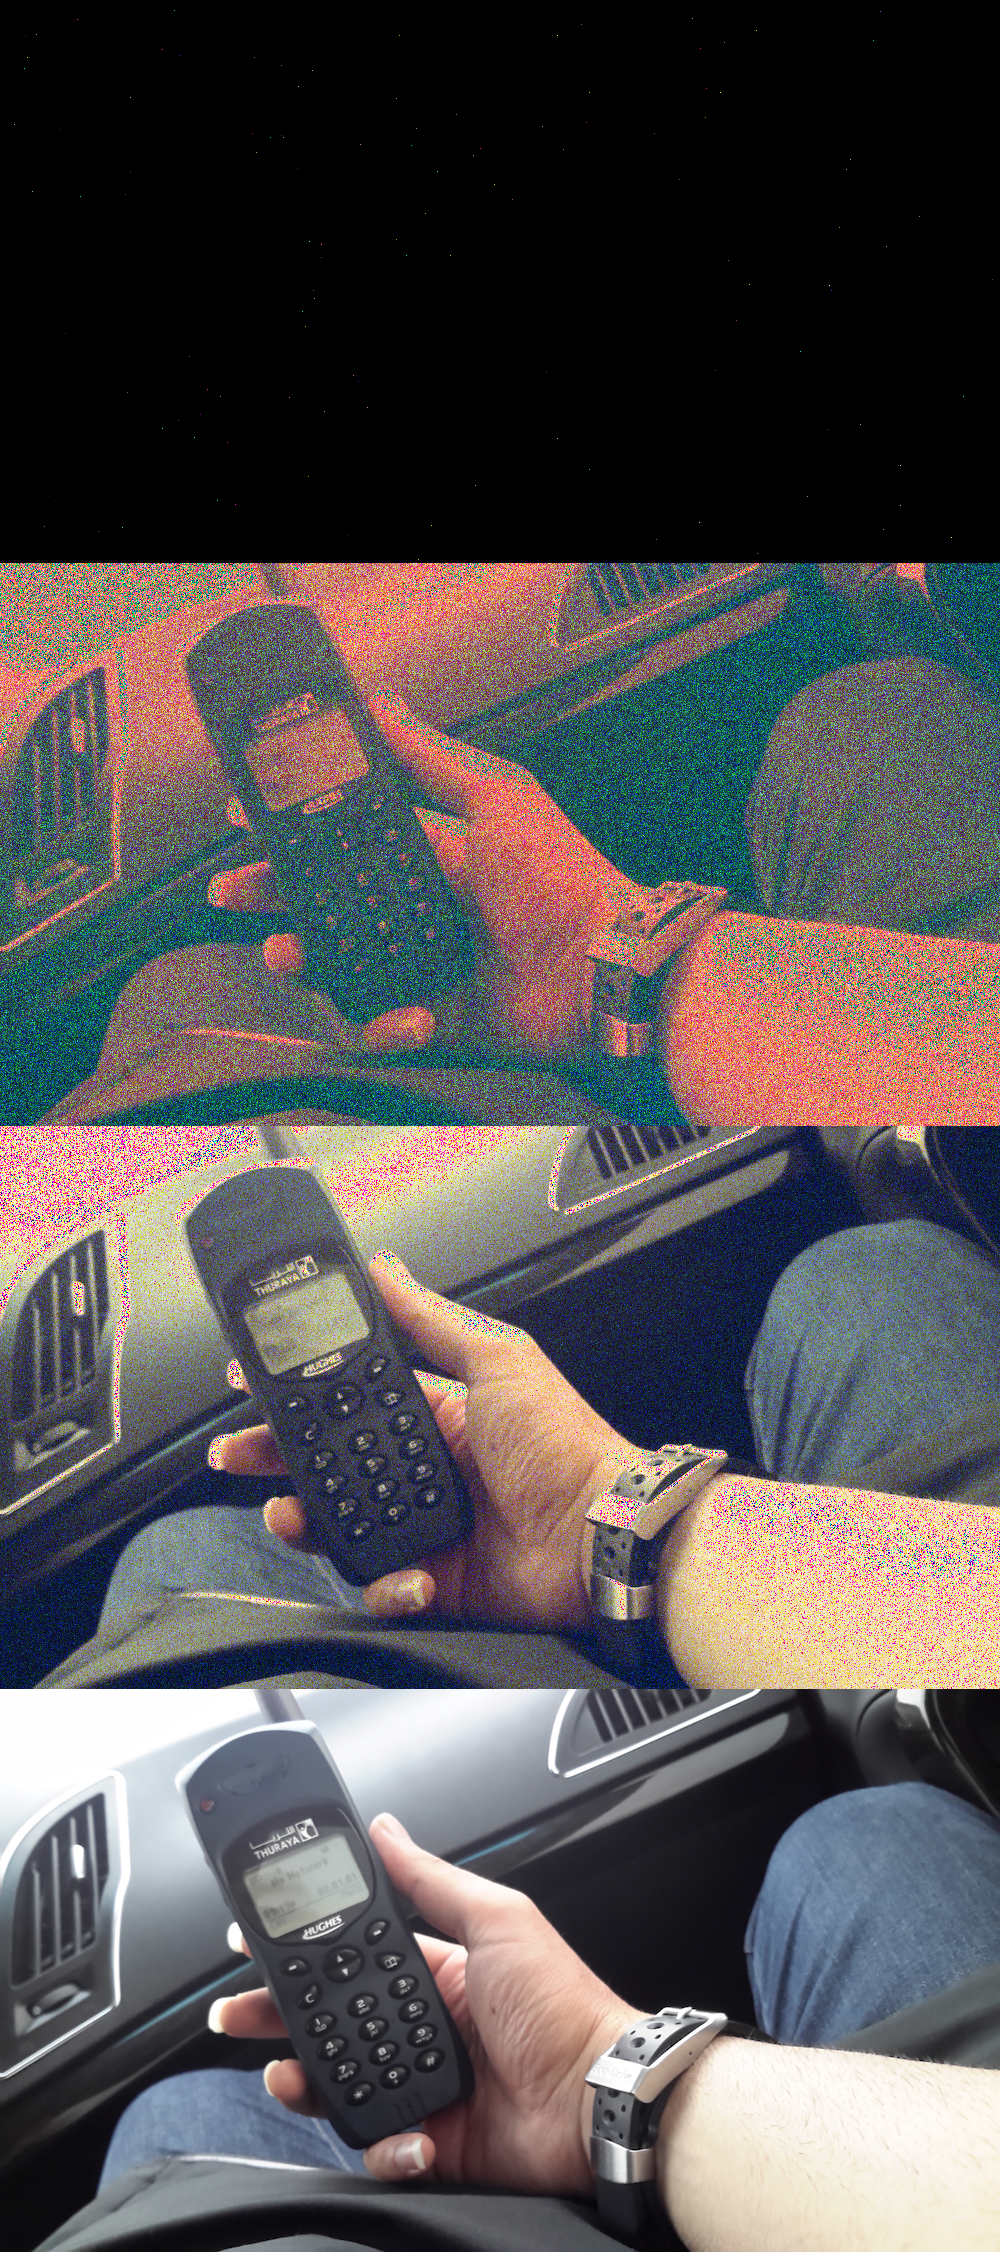
\includegraphics[width=1.0\textwidth,height=65em]{./images/wf_sat_phone/000_123_134_original.png}
    \caption{WF Using Coded Diffraction Patterns on the Sat Phone Image from Top to Buttom: After Initialization, 
	at Iteration $=123$, at Iteration $=134$, and the Original Image}
    \label{fig:wf_dc/0_121_inal}
  \end{figure}
  % \clearpage % End the page
}
\afterpage{%
  % \clearpage % Start a new page
  \thispagestyle{empty} % No header/footer on this page
  \begin{figure}[!htbp]
    \centering
	\captionsetup{justification=centering}
    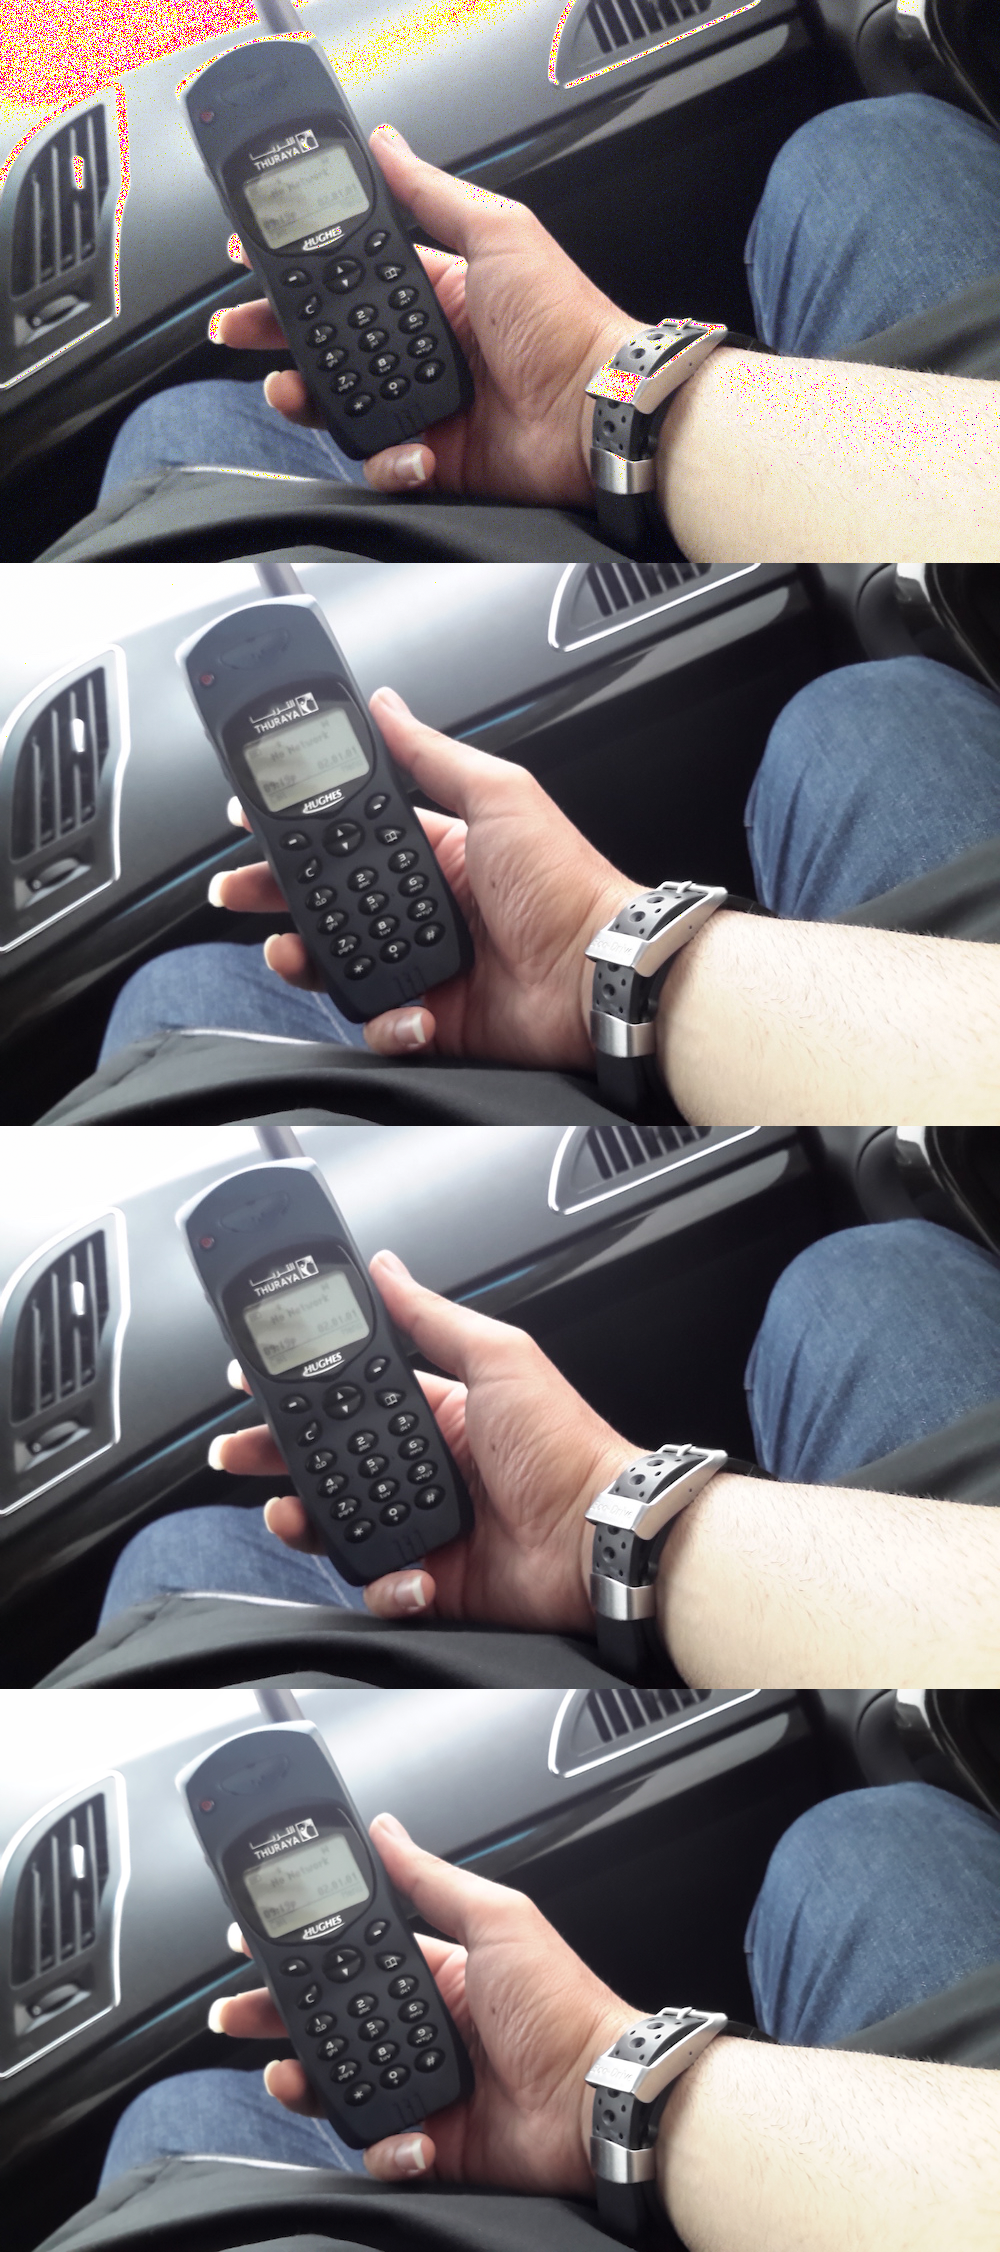
\includegraphics[width=1.0\textwidth,height=65em]{./images/wf_sat_phone/142_164_499_original.png}
    \caption{WF Using Coded Diffraction Patterns on the Sat Phone Image from Top to Buttom: At Iteration $=142$, 
	at Iteration $=164$, at Iteration $=499$, and the Original Image}
    % \label{fig:wf_dc/0_121_132riginal}
  \end{figure}
  % \clearpage % End the page
}
%%%%%%%%%%%%%%%%%%%%%%%%%%%%%%%%%%%%%%%%%%%%%%%%%%%%%%%%%%%%%
%%%%%%%%%%%%%%%%%% TWF Reconstruction %%%%%%%%%%%%%%%%%%%%%%%
%%%%%%%%%%%%%%%%%%%%%%%%%%%%%%%%%%%%%%%%%%%%%%%%%%%%%%%%%%%%%
\afterpage{%
  % \clearpage % Start a new page
  \thispagestyle{empty} % No header/footer on this page
  \begin{figure}[!htbp]
    \centering
	\captionsetup{justification=centering}
    \includegraphics[width=1.0\textwidth,height=65em]{./images/twf_sat_phone/000_008_012_original.png}
    \caption{TWF Using Coded Diffraction Patterns on the Sat Phone Image from Top to Buttom: After Initialization, at Iteration $=8$, at Iteration $=12$, and the Original Image}
    % \label{fig:wf356_1443563454}
  \end{figure}
  % \clearpage % End the page
}

\afterpage{%
  % \clearpage % Start a new page
  \thispagestyle{empty} % No header/footer on this page
  \begin{figure}[!htbp]
    \centering
	\captionsetup{justification=centering}
    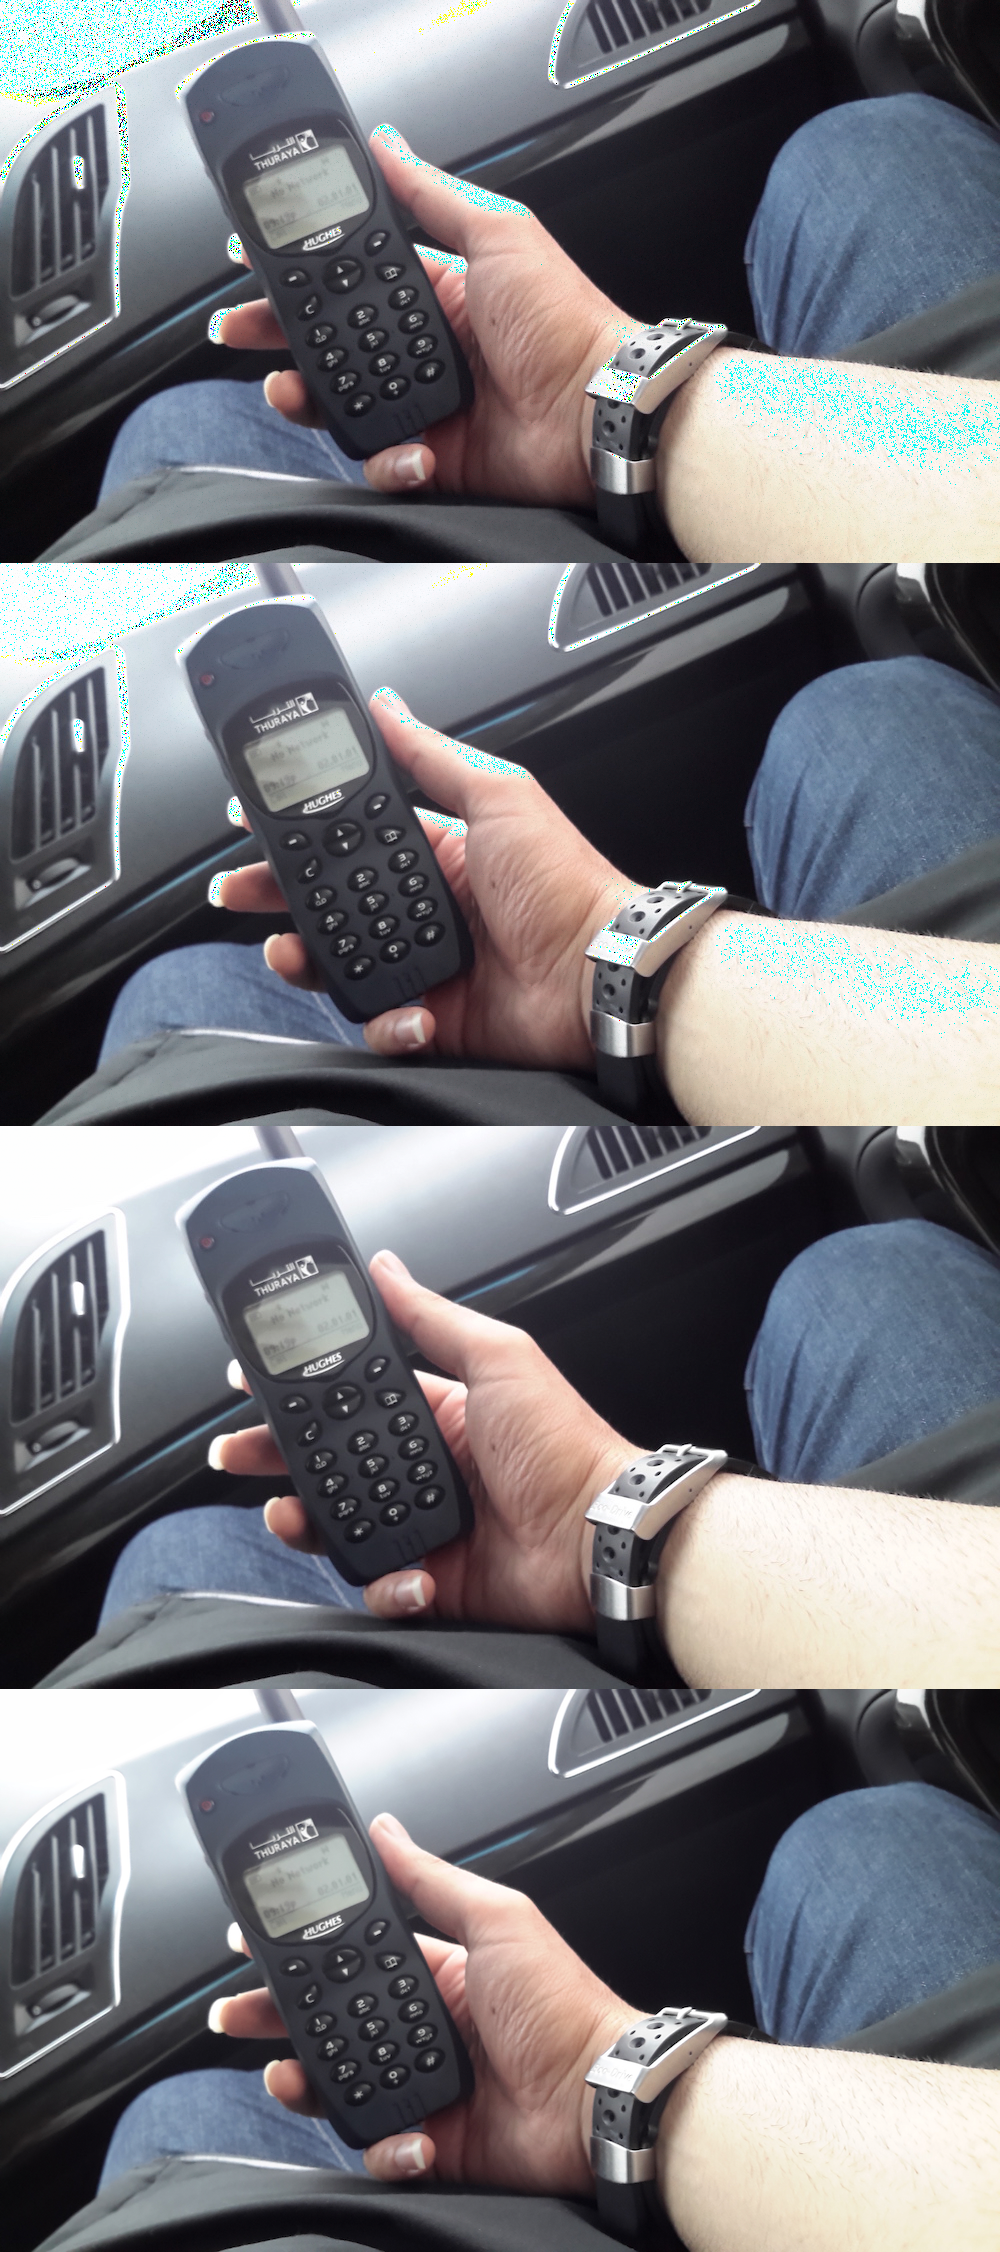
\includegraphics[width=1.0\textwidth,height=65em]{./images/twf_sat_phone/015_017_499_original.png}
    \caption{TWF Using Coded Diffraction Patterns on the Sat Phone Image from Top to Buttom: At Iteration $=15$, 
    at Iteration $=17$, at Iteration $=499$, and the Original Image}
    % \label{fig:wf_457143454}
  \end{figure}
  % \clearpage % End the page
}
%%%%%%%%%%%%%%%%%%%%%%%%%%%%%%%%%%%%%%%%%%%%%%%%%%%%%%%%%%%%%
%%%%%%%%%%%%%%%%%% RWF Reconstruction %%%%%%%%%%%%%%%%%%%%%%%
%%%%%%%%%%%%%%%%%%%%%%%%%%%%%%%%%%%%%%%%%%%%%%%%%%%%%%%%%%%%%
\afterpage{%
  % \clearpage % Start a new page
  \thispagestyle{empty} % No header/footer on this page
  \begin{figure}[!htbp]
    \centering
	\captionsetup{justification=centering}
    \includegraphics[width=1.0\textwidth,height=65em]{./images/rwf_sat_phone/000_025_32_original.png}
    \caption{RWF Using Coded Diffraction Patterns on the Sat Phone Image from Top to Buttom: After Initialization, at Iteration $=25$, at Iteration $=32$, and the Original Image}
    % \label{fig:wf356_1443563454}
  \end{figure}
  % \clearpage % End the page
}

\afterpage{%
  % \clearpage % Start a new page
  \thispagestyle{empty} % No header/footer on this page
  \begin{figure}[!htbp]
    \centering
	\captionsetup{justification=centering}
    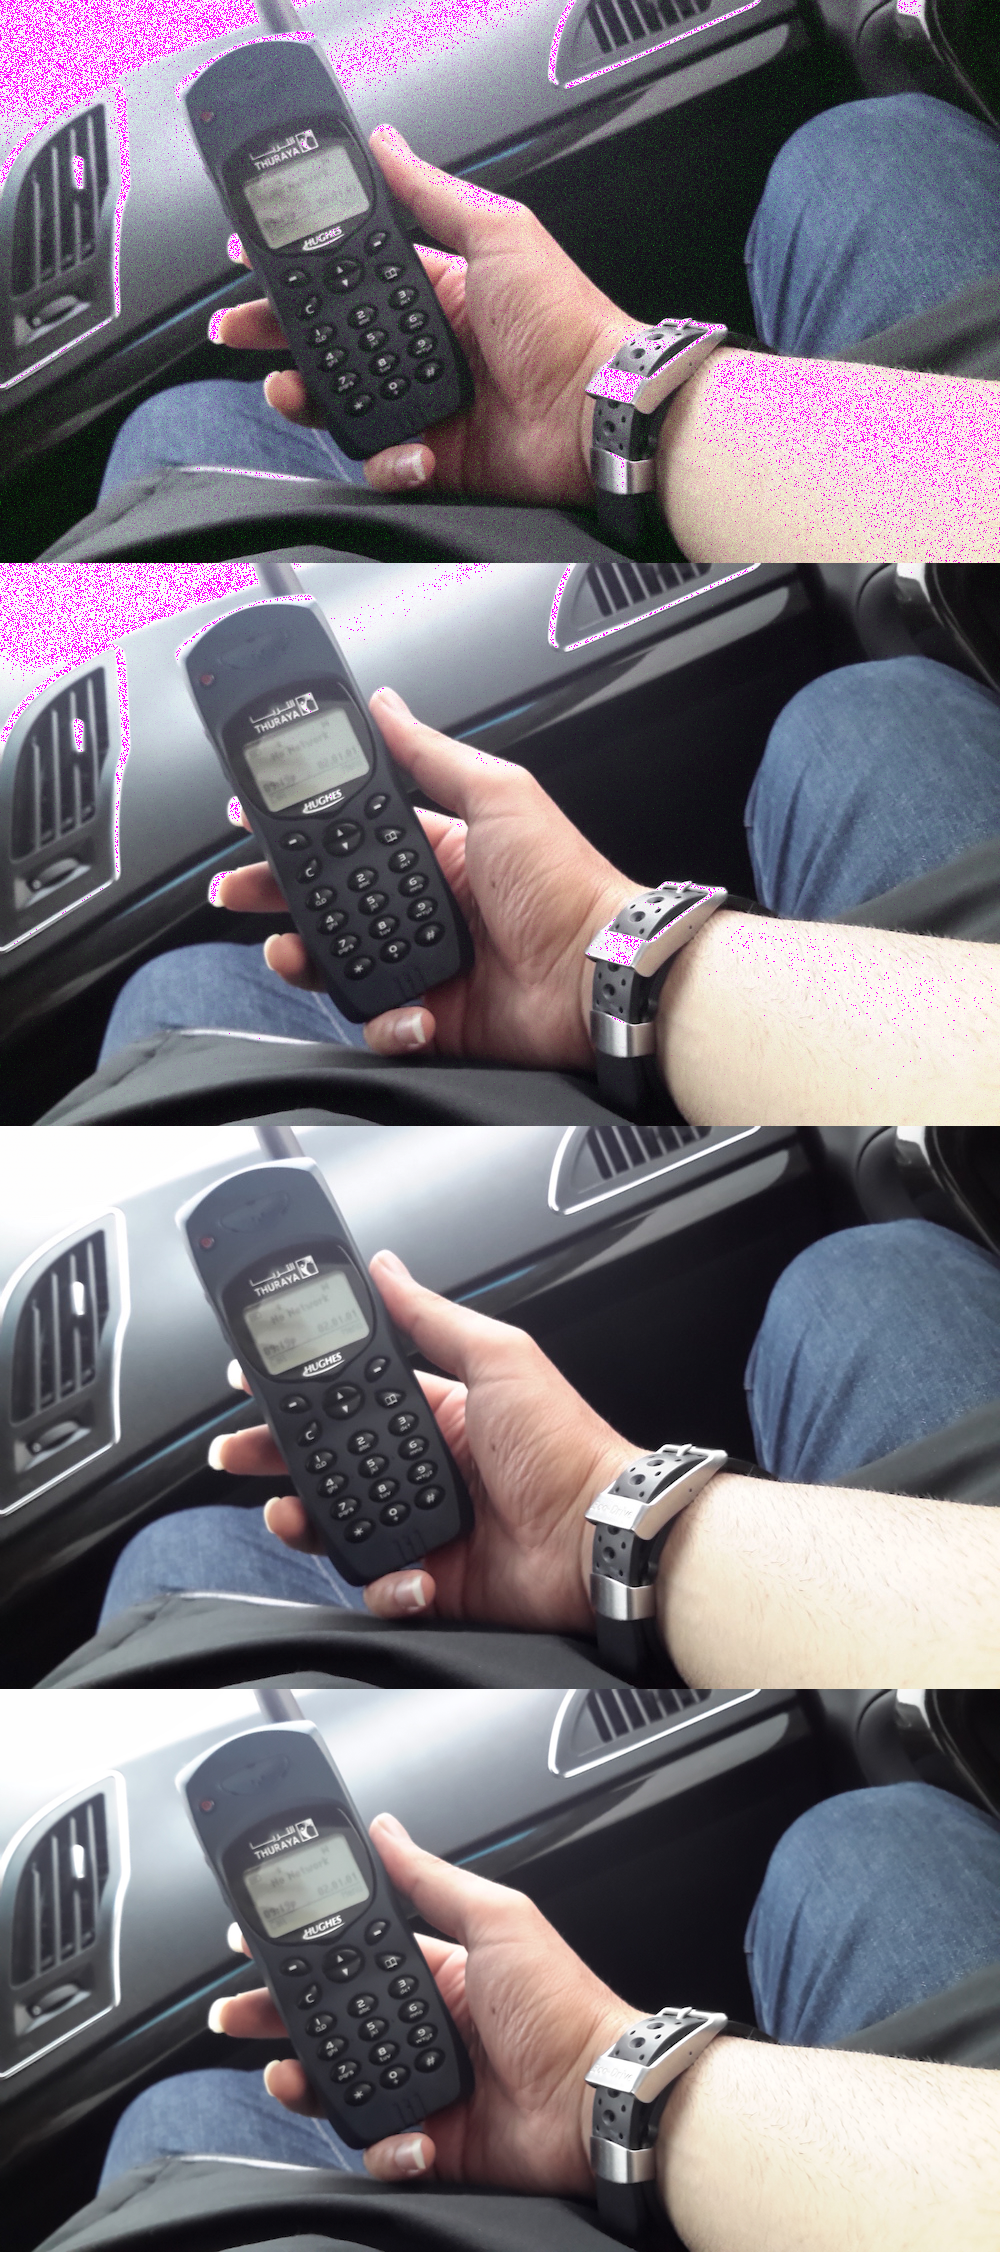
\includegraphics[width=1.0\textwidth,height=65em]{./images/rwf_sat_phone/034_037_499_original.png}
    \caption{RWF Using Coded Diffraction Patterns on the Sat Phone Image from Top to Buttom: At Iteration $=34$, 
    at Iteration $=37$, at Iteration $=499$, and the Original Image}
    % \label{fig:wf_457143454}
  \end{figure}
  % \clearpage % End the page
}
%%%%%%%%%%%%%%%%%%%%%%%%%%%%%%%%%%%%%%%%%%%%%%%%%%%%%%%%%%%%%
%%%%%%%%%%%% Unrolling an Iterative Algorithm  %%%%%%%%%%%%%%
%%%%%%%%%%%%%%%%%%%%%%%%%%%%%%%%%%%%%%%%%%%%%%%%%%%%%%%%%%%%%
\afterpage{%
  % \clearpage % Start a new page
  % \thispagestyle{empty} % No header/footer on this page
  \begin{figure}[!htbp]
    \centering
	\captionsetup{justification=centering}
  \begin{turn}{-90}
    
\begin{tikzpicture}[->,>=stealth',shorten >=1pt,auto,node distance=3cm,
  thick,c node/.style={circle,draw,
  ,minimum size=20mm},c_empt node/.style={circle,draw=none,
  ,minimum size=20mm},r node/.style={ rectangle,draw,
  ,minimum height=20mm,minimum width=30mm},a node/.style={single arrow, draw, rotate=0}]
  \node[r node] (Input_O) {Input};
  \node[c node] (Iteration)[above of=Input_O] {$h(.;\theta)$};
  \node[r node] (Output_O)[above of=Iteration] {Output};
  \node[a node] (Unrolling)[right of=Iteration] {Unrolling}; 
  \node[r node] (Input_U)[right of=Unrolling] {Input}; 
  \node[c node] (iter_1)[right of=Input_U] {$h^1(.;\theta^1)$}; 
  \node[c node] (iter_2)[right of=iter_1] {$h^2(.;\theta^2)$}; 
  \node[c_empt node] (dotdotdot)[right of=iter_2] {$\cdots\cdots$}; 
  \node[r node] (Output_U)[right of=dotdotdot] {Output};
  \node[r node] (interpretable)[below of=iter_2] {Interpretable Layers}; 
  \node[r node] (train)[above of=iter_2] {End to End Training}; 
  \path[every node/.style={font=\sffamily\small,
  		fill=white,inner sep=1pt}]
    (Input_O) edge [ left=30] node[left=1mm] {Preprocessing} (Iteration)    
    (Iteration) edge [loop left] node[left=1mm] {$k \rightarrow k+1$} (Iteration)
    (Iteration) edge [ left=30] node[left=1mm] {Post Processing} (Output_O)
    (Input_U) edge [ left=30] node[above=1mm] {} (iter_1)     
    (iter_1) edge [ left=30] node[above=1mm] {} (iter_2)     
    (iter_2) edge [ left=30] node[above=1mm] {} (dotdotdot)     
    (interpretable) edge [bend left=30] node[above=1mm] {} (iter_1)  
    (interpretable) edge [bend left=30] node[above=1mm] {} (iter_2)
    (train) edge [bend left=-25] node[above=1mm] {} (Input_U)
    (train) edge [bend left=30] node[above=1mm] {} (Output_U)
    ;     
\end{tikzpicture}

  \end{turn}
  \caption{The Unrolling Process of an Iterative Algorithm Schematically}
    \label{fig:unrolling}
  \end{figure}
  % \clearpage % End the page
}


%%%%%%%%%%%%%%%%%%%%%%%%%%%%%%%%%%%%%%%%%%%%%%%%%%%%%%%%%%%%%
%%%%%%%%%%%%%%%%%%%%% msip-Dell Specs %%%%%%%%%%%%%%%%%%%%%%%
%%%%%%%%%%%%%%%%%%%%%%%%%%%%%%%%%%%%%%%%%%%%%%%%%%%%%%%%%%%%%
\afterpage{%
  % \clearpage % Start a new page
  \begin{table}[!htbp]
    \centering
    \begin{tabular}{||l l||} 
     \hline
     General 		                	&  						                                                             \\ [0.5ex] 
     \hline\hline
     Processor 	         		 			& Intel\textregistered \space Xeon\textregistered         	                 \\
     Accelerator 			 	       		& NVIDIA\textregistered  	                                                 \\ 
     Operating System   			    & GNU/Linux(Ubuntu\textregistered) 	                                    	 \\
     Memory 	               			& 32617768 kB                                                              \\ [1ex] 
     \hline
     \hline
     Processor Details 	      		&  						                                                             \\ [0.5ex] 
     \hline\hline
     Architecture     			 			& X86\_64                                               	                 \\ 
     CPU op-mode(s)         			& 32-bit, 64-bit 	                                                         \\
     Address sizes                & 46 bits physical, 48 bits virtual  		                                   \\
     Byte Order                   & Little Endian  	                                                         \\ 
     CPU(s):                      & 8 	 	                                                                   \\
     On-line CPU(s) list:         & 0-7  	                                              	                   \\
     Vendor ID:                   & GenuineIntel\textregistered 	                         	                 \\
     Model name:                  & Intel\textregistered \space Xeon\textregistered CPU E5-1630 v3 at 3.70GHz \\
     Thread(s) per core:          & 2                                                                        \\
     Core(s) per socket:          & 4                                                   		                 \\
     Socket(s):                   & 1 	                                                	                   \\
     CPU max MHz:                 & 3800.0000 	                                         	                   \\
     CPU min MHz:                 & 1200.0000                                         	  	                 \\
     L1d Cache:                   & 128 KiB (4 instances)                           	    	                 \\
     L1i Cache:                   & 128 KiB (4 instances) 	 	                                               \\
     L2 Cache:                    & 1 MiB (4 instances) 	                                                   \\
     L3 Cache:                    & 10 MiB (1 instance) 	 	                                                 \\
     NUMA node(s):                & 1                                               	 	                     \\
     Optimization Flags           & Please Refer to the Intel\textregistered \space Brochure for the Details  		   \\[1ex] 
     \hline
     \hline
     Accelerator Details 			    &                                                                          \\[0.5ex] 
     \hline\hline
     Full Designation 	    			& NVIDIA\textregistered \space GeForce\textregistered \space RTX 2080 Ti 	               \\ 
     Memory   	              		& 11264 MiB 	                                           	                 \\
     CUDA Version:                & 12.2  	                                               	                 \\
     width:                       & 64 bits                                                                  \\
     clock:                       & 33 MHz 	                                                                 \\[1ex] 
     \hline
     \hline
     Numerical Framework Details	&  				                                            		                 \\[0.5ex] 
     \hline\hline
     python                       & 3.10.12                                                                  \\
     numpy                        & 1.25.2  		                                                             \\
     scipy                        & 1.11.1  		                                                             \\
     matplotlib                   & 3.7.2   		                                                             \\
     scikit-learn                 & 1.3.0  		                                                               \\
     scikit-image                 & 0.21.0  		                                                             \\
     pytorch                      & 2.0.0			 			 	                                                       \\ 
     pytorch-cuda                 & 11.7 	 	                                                                 \\
     \LaTeX \space Distribution   & \TeX-Live			 			 	                                                     \\
     \LaTeX \space Engine/Recipe  & Auto Recipe in VS-Code \LaTeX \space Extension		                       \\[1ex] 
     \hline
    \end{tabular}
    \caption{Software and Hardware that were used on the second system}
    % \label{tab:formulation}
    \end{table}
  % \clearpage % End the page
}
















%%%%%%%%%%%%%%%%%%%%%%%%%%%%%%%%%%%%%%%%%%%%%%%%%%%%%%%%%%%%%
%%%%%%%%%%%%%%%%%%% WF Variants Algorithms %%%%%%%%%%%%%%%%%%
%%%%%%%%%%%%%%%%%%%%%%%%%%%%%%%%%%%%%%%%%%%%%%%%%%%%%%%%%%%%%


%%%%%%%%%%%%%%%%%%%%%%%%%%%%%%%%%%%%%%%%%%%%%%%%%%%%%%%%%%%%%
%%%%%%%%%%%%%%%%%%%%%% Wirtinger Flow %%%%%%%%%%%%%%%%%%%%%%%
%%%%%%%%%%%%%%%%%%%%%%%%%%%%%%%%%%%%%%%%%%%%%%%%%%%%%%%%%%%%%
\afterpage{%
\clearpage % Start a new page
\begin{algorithm}[!htbp]
  \caption{\ac{WF}\index{WF} suggested by \cite{Candes2014}}
    \textbf{Input}: Let $\boldsymbol{y}=\{y_i\}_{i=1}^m$ and $\{\boldsymbol{a}_i\}_{i=1}^m$ be our measurements and sampling vectors; \\
    \textbf{Parameters}:  step size $\mu$;\\
    \textbf{Initialization}: Let $\hat{\boldsymbol{z}}$, be the eigenvector corresponding to the largest eigenvalue of:
    \begin{equation}
      \boldsymbol{Y} \coloneqq \frac{1}{m}\sum_{i=1}^m y_i\boldsymbol{a}_i \boldsymbol{a}_i^*\boldsymbol{1}
    \end{equation}
    and find it using power iteration. Let also $\Lambda=\sqrt{n\sum_{i=1}^m \frac{y_i}{\|\boldsymbol{a}_i\|_X^2}}$ to be the norm estimation of the signal of interest that we are trying to recover. 
    Set $\boldsymbol{z}^{(0)}=\Lambda\hat{\boldsymbol{z}}$ for the initialization.\\
    \textbf{Update loop}: for $t=0, \ldots ,t=T-1$ do the update as:
    \begin{flalign}
      \boldsymbol{z}^{(t+1)}=\boldsymbol{z}^{(t)}- \frac{\mu_{t+1}}{\left|z_0\right|_X^2}\left(\frac{1}{m}\sum_{i=1}^{m}\left(\left|\boldsymbol{a}_i^*\boldsymbol{z}^{(t)}\right|_X-y_i\right)\left(\boldsymbol{a}_i\boldsymbol{a}_i^*\right)\boldsymbol{z}^{(t)}\right).
    \end{flalign}
    \textbf{Output}: $\boldsymbol{z}^{(T)}$.
  \end{algorithm}
  \begin{itemize}
    \item Power iteration is described in almost any standard numerical linear algebra book like \cite{Trefethen2022}\cite{Demmel1997}\cite{Golub2013}. 
    \item If vectorized operations are still a thing in the future, try to formulate the algorithm in the most vectorized form possible in whatever 
    numerical framework you are using. For a first exposure to vectorized operations you can have a look at \cite{Hager2010}. For in depth understanding of 
    computer architecture that leads to the vectorized operations please refer to either \cite{Patterson2014} or \cite{Hennessy2019}.
    \item Try to port as much as computation possible from \ac{CPU} to accelerators like \ac{GPU}s and \ac{TPU}s if 
    your analysis on the porting confirms it to be worthwhile.
  \end{itemize}
  A possible \pytorch\cite{LFMAI2023} implementation using \ac{CUDA}\cite{Nvidia} is listed below as:
  % \lstinputlisting[language=Python, firstline=1,lastline=20]{./algorithms/wf.py}
  \lstinputlisting[language=Python]{./algorithms/wf.py}\index{WF}    
\clearpage % End the page
}


%%%%%%%%%%%%%%%%%%%%%%%%%%%%%%%%%%%%%%%%%%%%%%%%%%%%%%%%%%%%%
%%%%%%%%%%%%%%%%%% Truncated Wirtinger Flow %%%%%%%%%%%%%%%%%
%%%%%%%%%%%%%%%%%%%%%%%%%%%%%%%%%%%%%%%%%%%%%%%%%%%%%%%%%%%%%
\afterpage{%
\clearpage % Start a new page
\begin{algorithm}[!htbp]
  \caption{\ac{TWF}\index{TWF} suggested by \cite{Chen2015}}
    \textbf{Input}: Let $\boldsymbol{y}=\{y_i\}_{i=1}^m$ and $\{\boldsymbol{a}_i\}_{i=1}^m$ be our measurements and sampling vectors; \\
    \textbf{Parameters}: step size $\mu$, and thresholds $\alpha_{z}^{lb},\alpha_{z}^{ub},\alpha_{h},\alpha_{y}$;\\
    \textbf{Initialization}: Let $\hat{\boldsymbol{z}}$, be the eigenvector corresponding to the largest eigenvalue of:
    \begin{equation}
      \boldsymbol{Y} \coloneqq \frac{1}{m}\sum_{i=1}^m y_i\boldsymbol{a}_i \boldsymbol{a}_i^*\boldsymbol{1}_{\left\{\left|y_i\right|_X\leq \frac{\alpha_{y}^2\sum_{i=1}^{m}y_i}{m}\right\}}
    \end{equation}
    and find it using power iteration. Let also $\Lambda=\sqrt{n\sum_{i=1}^m \frac{y_i}{\|\boldsymbol{a}_i\|_X^2}}$ to be the norm estimation of the signal of interest that we are trying to recover. 
    Set $\boldsymbol{z}^{(0)}=\Lambda\hat{\boldsymbol{z}}$ for the initialization.\\
    \textbf{Update loop}: for $t=0, \ldots ,t=T-1$ do the update as:
    \begin{flalign}
      \boldsymbol{z}^{(t+1)}=\boldsymbol{z}^{(t)}- \frac{\mu_{t+1}}{{\boldsymbol{z}^{(t)}}^*\boldsymbol{a}_i}\left(\frac{1}{m}\sum_{i=1}^{m}2\left(\left|\boldsymbol{a}_i^*\boldsymbol{z}^{(t)}\right|_X^2-y_i\right)\boldsymbol{a}_i\boldsymbol{1}_{\mathcal{E}_1^i\cap\mathcal{E}_2^i}\right).
    \end{flalign}
    where
    \begin{equation*}
      \begin{split}
        \mathcal{E}_1^i &\coloneqq \left\{  \alpha_z^{lb}  \leq \frac{\sqrt{n}\left|\boldsymbol{a}_i^*\boldsymbol{z}^{(t)}\right|_X}{\left|\boldsymbol{a}_i\right|_X\left|\boldsymbol{z}^{(t)}\right|_X} \leq  \alpha_z^{ub}   \right\} \\
        \mathcal{E}_2^i &\coloneqq \left\{ \left|y_i-\left|\boldsymbol{a}_i^*\boldsymbol{z}^{(t)}\right|_X^2\right| \leq  \alpha_h{K_t}\frac{\sqrt{n}\left|\boldsymbol{a}_i^*\boldsymbol{z}^{(t)}\right|_X}{\left|\boldsymbol{a}_i\right|_X\left|\boldsymbol{z}^{(t)}\right|_X}   \right\} \\
        K_t             &\coloneqq \frac{1}{m}\sum_{j=1}^{m}\left|y_j-\left|\boldsymbol{a}_i^*\boldsymbol{z}^{(t)}\right|_X^2\right|
      \end{split}
    \end{equation*}
    \textbf{Output}: $\boldsymbol{z}^{(T)}$.
  \end{algorithm}
  \begin{itemize}
    \item Power iteration is described in almost any standard numerical linear algebra book like \cite{Trefethen2022}\cite{Demmel1997}\cite{Golub2013}. 
    \item If vectorized operations are still a thing in the future, try to formulate the algorithm in the most vectorized form possible in whatever 
    numerical framework you are using. For a first exposure to vectorized operations you can have a look at \cite{Hager2010}. For in depth understanding of 
    computer architecture that leads to the vectorized operations please refer to either \cite{Patterson2014} or \cite{Hennessy2019}.
    \item Try to port as much as computation possible from \ac{CPU} to accelerators like \ac{GPU}s and \ac{TPU}s if 
    your analysis on the porting confirms it to be worthwhile.
  \end{itemize}
  A possible \pytorch\cite{LFMAI2023} implementation using \ac{CUDA}\cite{Nvidia} is listed below as:
  % \lstinputlisting[language=Python, firstline=1,lastline=20]{./algorithms/twf.py}
  \lstinputlisting[language=Python]{./algorithms/twf.py}\index{TWF}    
\clearpage % End the page
}

%%%%%%%%%%%%%%%%%%%%%%%%%%%%%%%%%%%%%%%%%%%%%%%%%%%%%%%%%%%%%
%%%%%%%%%%%%%%%%%%% Reshaped Wirtinger Flow %%%%%%%%%%%%%%%%%
%%%%%%%%%%%%%%%%%%%%%%%%%%%%%%%%%%%%%%%%%%%%%%%%%%%%%%%%%%%%%
\afterpage{%
\clearpage % Start a new page
\begin{algorithm}[!htbp]
  \caption{\ac{RWF}\index{RWF} suggested by \cite{Zhang2016}}
    \textbf{Input}: Let $\boldsymbol{y}=\{y_i\}_{i=1}^m$ and $\{\boldsymbol{a}_i\}_{i=1}^m$ be our measurements and sampling vectors; \\
    \textbf{Parameters:}  step size $\mu$, and thresholds $\alpha_{l},\alpha_{u}$;\\
    \textbf{Initialization}: Let $\hat{\boldsymbol{z}}$, be the eigenvector corresponding to the largest eigenvalue of:
    \begin{equation}
      \boldsymbol{Y} \coloneqq \frac{1}{m}\sum_{i=1}^m y_i\boldsymbol{a}_i \boldsymbol{a}_i^*\boldsymbol{1}_{\left\{ \alpha_{l}n\sum_{i=1}^m \frac{y_i}{\|\boldsymbol{a}_i\|_1} \leq \left|y_i\right|_X \alpha_{u}n\sum_{i=1}^m \frac{y_i}{\|\boldsymbol{a}_i\|_1}\right\}}
    \end{equation}
    and find it using power iteration. Let also $\Lambda=n\sum_{i=1}^m \frac{y_i}{\|\boldsymbol{a}_i\|_1}$ to be the norm estimation of the signal of interest that we are trying to recover. 
    Set $\boldsymbol{z}^{(0)}=\Lambda\hat{\boldsymbol{z}}$ for the initialization.\\
    \textbf{Update loop}: for $t=0, \ldots ,t=T-1$ do the update as:
    \begin{flalign}
      \boldsymbol{z}^{(t+1)}=\boldsymbol{z}^{(t)}- \mu_{t+1}\left(\frac{1}{m}\sum_{i=1}^{m}\left(\boldsymbol{a}_i^*\boldsymbol{z}^{(t)}-y_i\frac{\boldsymbol{a}_i^*\boldsymbol{z}^{(t)}}{\left|\boldsymbol{a}_i^*\boldsymbol{z}^{(t)}\right|_X}\right)\boldsymbol{a}_i\right).
    \end{flalign}
    \textbf{Output}: $\boldsymbol{z}^{(T)}$.
  \end{algorithm}
  \begin{itemize}
    \item Power iteration is described in almost any standard numerical linear algebra book like \cite{Trefethen2022}\cite{Demmel1997}\cite{Golub2013}. 
    \item If vectorized operations are still a thing in the future, try to formulate the algorithm in the most vectorized form possible in whatever 
    numerical framework you are using. For a first exposure to vectorized operations you can have a look at \cite{Hager2010}. For in depth understanding of 
    computer architecture that leads to the vectorized operations please refer to either \cite{Patterson2014} or \cite{Hennessy2019}.
    \item Try to port as much as computation possible from \ac{CPU} to accelerators like \ac{GPU}s and \ac{TPU}s if 
    your analysis on the porting confirms it to be worthwhile.
  \end{itemize}
  A possible \pytorch\cite{LFMAI2023} implementation using \ac{CUDA}\cite{Nvidia} is listed below as:
  % \lstinputlisting[language=Python, firstline=1,lastline=20]{./algorithms/rwf.py}
  \lstinputlisting[language=Python]{./algorithms/rwf.py}\index{RWF}    
\clearpage % End the page
}
%%%%%%%%%%%%%%%%%%%%%%%%%%%%%%%%%%%%%%%%%%%%%%%%%%%%%%%%%%%%%
%%%%%%%%%%% Incrementally Reshaped Wirtinger Flow %%%%%%%%%%%
%%%%%%%%%%%%%%%%%%%%%%%%%%%%%%%%%%%%%%%%%%%%%%%%%%%%%%%%%%%%%
\afterpage{%
\clearpage % Start a new page
\begin{algorithm}[!htbp]
  \caption{\ac{IRWF}\index{IRWF} suggested by \cite{Zhang2016}}
    \textbf{Input}: Let $\boldsymbol{y}=\{y_i\}_{i=1}^m$ and $\{\boldsymbol{a}_i\}_{i=1}^m$ be our measurements and sampling vectors; \\
    \textbf{Parameters:}  step size $\mu$, and thresholds $\alpha_{l},\alpha_{u}$;\\
    \textbf{Initialization}: Let $\hat{\boldsymbol{z}}$, be the eigenvector corresponding to the largest eigenvalue of:
    \begin{equation}
      \boldsymbol{Y} \coloneqq \frac{1}{m}\sum_{i=1}^m y_i\boldsymbol{a}_i \boldsymbol{a}_i^*\boldsymbol{1}_{\left\{ \alpha_{l}n\sum_{i=1}^m \frac{y_i}{\|\boldsymbol{a}_i\|_1} \leq \left|y_i\right|_X \alpha_{u}n\sum_{i=1}^m \frac{y_i}{\|\boldsymbol{a}_i\|_1}\right\}}
    \end{equation}
    and find it using power iteration. Let also $\Lambda=n\sum_{i=1}^m \frac{y_i}{\|\boldsymbol{a}_i\|_1}$ to be the norm estimation of the signal of interest that we are trying to recover. 
    Set $\boldsymbol{z}^{(0)}=\Lambda\hat{\boldsymbol{z}}$ for the initialization.\\
    \textbf{Update loop}: for $t=0, \ldots ,t=T-1$ do the update as:
    \begin{flalign}
      \boldsymbol{z}^{(t+1)}=\boldsymbol{z}^{(t)}- \mu_{t+1}\left(\frac{1}{m}\sum_{i=1}^{m}\left(\boldsymbol{a}_{i_t}^*\boldsymbol{z}^{(t)}-y_{i_t}\frac{\boldsymbol{a}_{i_t}^*\boldsymbol{z}^{(t)}}{\left|\boldsymbol{a}_{i_t}^*\boldsymbol{z}^{(t)}\right|_X}\right)\boldsymbol{a}_i\right).
    \end{flalign}
    where $i_t$ is randomly selected from the set $\left\{1,\cdots,m\right\}$.\\
    \textbf{Output}: $\boldsymbol{z}^{(T)}$.
  \end{algorithm}
  \begin{itemize}
    \item Power iteration is described in almost any standard numerical linear algebra book like \cite{Trefethen2022}\cite{Demmel1997}\cite{Golub2013}. 
    \item If vectorized operations are still a thing in the future, try to formulate the algorithm in the most vectorized form possible in whatever 
    numerical framework you are using. For a first exposure to vectorized operations you can have a look at \cite{Hager2010}. For in depth understanding of 
    computer architecture that leads to the vectorized operations please refer to either \cite{Patterson2014} or \cite{Hennessy2019}.
    \item Try to port as much as computation possible from \ac{CPU} to accelerators like \ac{GPU}s and \ac{TPU}s if 
    your analysis on the porting confirms it to be worthwhile.
  \end{itemize}
  A possible PyTorch\cite{LFMAI2023} implementation using \ac{CUDA}\cite{Nvidia} is listed below as:
  % \lstinputlisting[language=Python, firstline=1,lastline=20]{./algorithms/wf.py}
  \lstinputlisting[language=Python]{./algorithms/irwf.py}\index{IRWF}    
\clearpage % End the page
}
%%%%%%%%%%%%%%%%%%%%%%%%%%%%%%%%%%%%%%%%%%%%%%%%%%%%%%%%%%%%%
%%%%% Incrementally Mini-Batch Reshaped Wirtinger Flow %%%%%%
%%%%%%%%%%%%%%%%%%%%%%%%%%%%%%%%%%%%%%%%%%%%%%%%%%%%%%%%%%%%%
\afterpage{%
\clearpage % Start a new page
\begin{algorithm}[!htbp]
  \caption{\ac{IMRWF}\index{IMRWF} suggested by \cite{Zhang2016}}
    \textbf{Input}: Let $\boldsymbol{y}=\{y_i\}_{i=1}^m$ and $\{\boldsymbol{a}_i\}_{i=1}^m$ be our measurements and sampling vectors; \\
    \textbf{Parameters:}  step size $\mu$, and thresholds $\alpha_{l},\alpha_{u}$, batch size $k$;\\
    \textbf{Initialization}: Let $\hat{\boldsymbol{z}}$, be the eigenvector corresponding to the largest eigenvalue of:
    \begin{equation}
      \boldsymbol{Y} \coloneqq \frac{1}{m}\sum_{i=1}^m y_i\boldsymbol{a}_i \boldsymbol{a}_i^*\boldsymbol{1}_{\left\{ \alpha_{l}n\sum_{i=1}^m \frac{y_i}{\|\boldsymbol{a}_i\|_1} \leq \left|y_i\right|_X \alpha_{u}n\sum_{i=1}^m \frac{y_i}{\|\boldsymbol{a}_i\|_1}\right\}}
    \end{equation}
    and find it using power iteration. Let also $\Lambda=n\sum_{i=1}^m \frac{y_i}{\|\boldsymbol{a}_i\|_1}$ to be the norm estimation of the signal of interest that we are trying to recover. 
    Set $\boldsymbol{z}^{(0)}=\Lambda\hat{\boldsymbol{z}}$ for the initialization.\\
    \textbf{Update loop}: for $t=0, \ldots ,t=T-1$ do the update as:
    \begin{flalign}
      \boldsymbol{z}^{(t+1)}=\boldsymbol{z}^{(t)}- \mu_{t+1}\boldsymbol{A}_{\Gamma_t}\left(\boldsymbol{A}_{\Gamma_t}\boldsymbol{z}^{(t)}-\boldsymbol{y}_{\Gamma_t} \odot \frac{\boldsymbol{A}_{\Gamma_t}\boldsymbol{z}^{(t)}}{\left|\boldsymbol{A}_{\Gamma_t}\boldsymbol{z}^{(t)}\right|_{e_X}}\right).
    \end{flalign}
    where $\Gamma_t$, the index vector, is randomly selected from the subsets of $\left\{1,\cdots,m\right\}$ that has $k$ members. $\boldsymbol{A}_{\Gamma_t}, \boldsymbol{y}_{\Gamma_t}$ 
    correspond to the index vector taken from the original $\boldsymbol{A}$ and $\boldsymbol{y}$ \\
    \textbf{Output}: $\boldsymbol{z}^{(T)}$.
  \end{algorithm}
  \begin{itemize}
    \item Power iteration is described in almost any standard numerical linear algebra book like \cite{Trefethen2022}\cite{Demmel1997}\cite{Golub2013}. 
    \item If vectorized operations are still a thing in the future, try to formulate the algorithm in the most vectorized form possible in whatever 
    numerical framework you are using. For a first exposure to vectorized operations you can have a look at \cite{Hager2010}. For in depth understanding of 
    computer architecture that leads to the vectorized operations please refer to either \cite{Patterson2014} or \cite{Hennessy2019}.
    \item Try to port as much as computation possible from \ac{CPU} to accelerators like \ac{GPU}s and \ac{TPU}s if 
    your analysis on the porting confirms it to be worthwhile.
  \end{itemize}
  A possible \pytorch\cite{LFMAI2023} implementation using \ac{CUDA}\cite{Nvidia} is listed below as:
  % \lstinputlisting[language=Python, firstline=1,lastline=20]{./algorithms/wf.py}
  \lstinputlisting[language=Python]{./algorithms/imrwf.py}\index{IMRWF}    
\clearpage % End the page
}